% REMEMBER: You must not plagiarise anything in your report. Be extremely careful.

\documentclass{l4proj}
\newcommand{\type}{\mathsf{type}}
\newcommand{\passivetype}{\mathsf{passiveT}}

\newcommand{\phrasetype}{\mathsf{phrase}}
\newcommand{\passivephrasetype}{\mathsf{passivePhrase}}
\newcommand{\access}{\mathsf{access}}
\newcommand{\datatype}{\mathsf{data}}
\newcommand{\natkind}{\mathsf{nat}}
\newcommand{\addrkind}{\mathsf{addrSpace}}
\newcommand{\ntnkind}{\natkind\hspace{-.25em}\rightarrow\hspace{-.25em}\natkind}
\newcommand{\ntdkind}{\natkind\hspace{-.25em}\rightarrow\hspace{-.25em}\datatype}
\newcommand{\vwkind}{\mathsf{width}}
\newcommand{\readacc}{\mathtt{R}}
\newcommand{\writeacc}{\mathtt{W}}
\newcommand{\num}{\mathsf{num}}
\newcommand{\sem}[1]{\llbracket #1 \rrbracket}
\newcommand{\interfere}{\mathrel\triangledown}
\newcommand{\indep}{\mathrel\triangle}
\newcommand{\objspace}{\mathord{\dagger}}
\newcommand{\basic}{\mathsf{basic}}

\newcommand{\kw}[1]{\mathrm{#1}}

\newcommand{\tyval}[2]{\ensuremath{#1_{#2}}}
\newcommand{\tycomm}{\mathsf{comm}}
\newcommand{\tyexp}[2]{\mathsf{exp}[#1, #2]}
\newcommand{\typush}{\mathsf{push}}
\newcommand{\tymem}{\mathsf{mem}}
\newcommand{\tyacc}[1]{\mathsf{acc}[#1]}
\newcommand{\tyvar}{\mathsf{var}}
\newcommand{\tyidx}{\mathsf{idx}}

% \usepackage{fdsymbol}

\newcommand{\lArray}[2]{#1\scalebox{.9}{\text{\raisebox{-.25em}{$\bullet$}}}#2}
\newcommand{\lDepArray}[2]{#1\scalebox{.5}{\text{\raisebox{-.25em}{$\blacksquare$}}}#2}
\newcommand{\lVector}[2]{\left<#1\right>#2}
\newcommand{\lPair}[2]{#1 \times #2}
\newcommand{\lNtDT}[2]{#1\mapsto#2}
\newcommand{\lNtN}[2]{#1\mapsto#2}

\newcommand{\pureto}{\to_{\textrm{p}}}

\newcommand{\multiset}[1]{\lbag #1 \rbag}

\newcommand{\DPIA}{\ensuremath{\mathsf{DPIA}}\xspace}
\newcommand{\IA}{\ensuremath{\mathsf{IA}}\xspace}

% judgements
\newcommand{\typ}[5]{#1 \mid #2; #3 \vdash #4 : #5}
\newcommand{\typd}{\typ{\Delta}}

\newcommand{\semA}[1]{\mathcal{A}\llparenthesis #1 \rrparenthesis}
\newcommand{\semM}[2]{\mathcal{M}(#1, |#2|)}
\newcommand{\semE}[1]{\mathcal{C}\llparenthesis #1 \rrparenthesis}

\newcommand{\projone}[1]{#1.1}
\newcommand{\projtwo}[1]{#1.2}

\newcommand{\prim}[1]{\bm{\mathsf{#1}}}

\newcommand{\mapI}{\ensuremath{\prim{mapI}}\xspace}
\newcommand{\reduceI}{\ensuremath{\prim{reduceI}}\xspace}

%% object variables for data types
%% \newcommand{\dt}{\delta}
%% \newcommand{\dtone}{\delta_1}
%% \newcommand{\dttwo}{\delta_2}

%% \newcommand{\dt}{d}
%% \newcommand{\dtone}{d_1}
%% \newcommand{\dttwo}{d_2}

% meta variables

% access
\newcommand{\W}{\omega}
\newcommand{\Wone}{\omega_1}
\newcommand{\Wtwo}{\omega_2}

% addrSpace
\newcommand{\A}{\alpha}
\newcommand{\Aone}{\alpha_1}
\newcommand{\Atwo}{\alpha_2}

% nat->nat
\newcommand{\FN}{F_\N}
\newcommand{\FNone}{F_\None}
\newcommand{\FNtwo}{F_\Ntwo}

% nat->data
\newcommand{\FDT}{F_\DT}
\newcommand{\FDTone}{F_\DTone}
\newcommand{\FDTtwo}{F_\DTtwo}

% nat
\newcommand{\Nat}[1]{#1}
\newcommand{\N}{\Nat{N}}

% data
\newcommand{\DT}{T}
\newcommand{\DTone}{S}
\newcommand{\DTtwo}{T}

% type
\newcommand{\TY}{\theta}
\newcommand{\TYone}{\theta_1}
\newcommand{\TYtwo}{\theta_2}

% variables

% expression values
\newcommand{\x}{x}
\newcommand{\xone}{x}
\newcommand{\xtwo}{y}

\newcommand{\Prog}{P}
\newcommand{\Progone}{P}
\newcommand{\Progtwo}{Q}

% access
\newcommand{\wvar}{w}
\newcommand{\wvarone}{w_1}
\newcommand{\wvartwo}{w_2}

% addrSpace
\newcommand{\avar}{a}
\newcommand{\avarone}{a_1}
\newcommand{\avartwo}{a_2}

% nat->nat
\newcommand{\fn}{f_\N}
\newcommand{\fnone}{f_\None}
\newcommand{\fntwo}{f_\Ntwo}

% nat->data
\newcommand{\fdt}{f_\DT}
\newcommand{\fdtone}{f_\DTone}
\newcommand{\fdttwo}{f_\DTtwo}

% nat
\newcommand{\nat}[1]{#1}
\newcommand{\n}{\nat{n}}
\newcommand{\m}{\nat{m}}

% data
\newcommand{\dt}{t}
\newcommand{\dtone}{s}
\newcommand{\dttwo}{t}
\newcommand{\dtzero}{r}



\newcommand{\ie}{\emph{i.e.},\xspace}
\newcommand{\eg}{\emph{e.g.},\xspace}
\newcommand{\etal}{et al.\xspace}

% comments
\newcommand{\Comment}[2]{{\par\noindent\small\color{red} \framebox{\parbox{\dimexpr\linewidth-2\fboxsep-2\fboxrule}{\textbf{#1:} #2}}}}
\newcommand{\todo}[1]{\Comment{TODO}{#1}}

\newcommand{\sam}[1]{\Comment{Sam}{#1}}

\newcommand{\mathrightfill}{\hskip \textwidth minus \textwidth \strut}

% shading
\definecolor{shade}{RGB}{223,223,223}
\newcommand\shade[1]{\setlength{\fboxsep}{0pt}\colorbox{shade}{\ensuremath{#1}}}

% environments
\renewenvironment{displaymath}{\small\[}{\]\normalsize\ignorespacesafterend}
\newenvironment{smallequation}{\small\begin{equation}}{\end{equation}\normalsize\ignorespacesafterend}

% possessive citation, i.e.: This is Adam's [1999] paper.
\newcommand\citeapos[1]{\citeauthor{#1}'s \citeyear{#1}}

\makeatletter % allow us to mention @-commands
\def\arcr{\@arraycr}
\makeatother
    
%
% put any additional packages here
%
\usepackage{array}
\usepackage{sansmath}
\usepackage{mathtools}
\usepackage{bm}
% for typing rules
\usepackage{mathpartir}

% config agda
\usepackage{agda}
\usepackage[utf8]{inputenc}
\usepackage{microtype}
\DisableLigatures[-]{encoding=T1}
\usepackage{newunicodechar}
\newunicodechar{λ}{\ensuremath{\mathnormal\lambda}}
\newunicodechar{ℕ}{\ensuremath{\mathbb{N}}}
\newunicodechar{∷}{\ensuremath{\mathnormal::}}
\newunicodechar{∀}{\ensuremath{\mathnormal\forall}}
\newunicodechar{→}{\ensuremath{\mathnormal\to}}
\newunicodechar{₁}{\ensuremath{\mathnormal{_1}}}
\newunicodechar{₂}{\ensuremath{\mathnormal{_2}}}
\newunicodechar{₃}{\ensuremath{\mathnormal{_3}}}
\newunicodechar{₄}{\ensuremath{\mathnormal{_4}}}
\newunicodechar{ε}{\ensuremath{\mathnormal\varepsilon}}
\newunicodechar{⊕}{\ensuremath{\mathnormal\oplus}}
\newunicodechar{ˡ}{\ensuremath{\mathnormal{^l}}}
\newunicodechar{ʳ}{\ensuremath{\mathnormal{^r}}}
\newunicodechar{ᵀ}{\ensuremath{\mathnormal{^T}}}
\newunicodechar{≡}{\ensuremath{\mathnormal\equiv}}
\newunicodechar{≅}{\ensuremath{\mathnormal{\cong}}}
\newunicodechar{∘}{\ensuremath{\mathnormal\circ}}
\newunicodechar{∎}{\ensuremath{\mathnormal\blacksquare}}
\newunicodechar{⟨}{\ensuremath{\langle}}
\newunicodechar{⟩}{\ensuremath{\rangle}}
\newunicodechar{′}{\ensuremath{\mathnormal{^\prime}}}
\newunicodechar{α}{\ensuremath{\mathnormal{\alpha}}}
\newunicodechar{β}{\ensuremath{\mathnormal{\beta}}}
\newunicodechar{γ}{\ensuremath{\mathnormal{\gamma}}}

\usepackage{inconsolata}
\lstset{
    literate={ℕ}{{\ensuremath{\mathbb{N}}}}1,
}

\begin{document}

%==============================================================================
%% METADATA
\title{Proving the Correctness of Rewrite Rules in LIFT's Rewrite-Based System}
\author{Xueying Qin}
\date{February 17, 2020}

\maketitle

%==============================================================================
%% ABSTRACT
\begin{abstract}
Rewrite rules in LIFT are used for generating optimised code but their correctness is not fully justified. In this project, mechanical proofs are developed in Agda for the verification of their correctness. Semantics of LIFT's data types and primitives are defined and their correctness are justified. Most of LIFT's rewrite rules are proven to be correct while some incorrect and inaccurate rules are fixed and clarified. Strategies of proving rewrite rules over array and multi-dimensional array operations are also discussed.
\end{abstract}

%==============================================================================

% EDUCATION REUSE CONSENT FORM
% If you consent to your project being shown to future students for educational purposes
% then insert your name and the date below to  sign the education use form that appears in the front of the document. 
% You must explicitly give consent if you wish to do so.
% If you sign, your project may be included in the Hall of Fame if it scores particularly highly.
%
% Please note that you are under no obligation to sign 
% this declaration, but doing so would help future students.

\def\consentname {Xueying Qin} % your full name
\def\consentdate {30 March 2020} % the date you agree
%
\educationalconsent
\renewcommand{\abstractname}{Acknowledgements}
\begin{abstract}
I would like to thank my supervisor Dr. Michel Steuwer, for his support and help in this project. Also, I would like to thank Uma Zalakain and Rongxiao Fu, who are PhD students at University of Glasgow, for sharing their experiences in developing verification programs in Agda, which are very helpful to this project.

\end{abstract}

%==============================================================================
\tableofcontents

%==============================================================================
%% Notes on formatting
%==============================================================================
% The first page, abstract and table of contents are numbered using Roman numerals and are not
% included in the page count. 
%
% From now on pages are numbered
% using Arabic numerals. Therefore, immediately after the first call to \chapter we need the call
% \pagenumbering{arabic} and this should be called once only in the document. 
%
% Do not alter the bibliography style.
%
% The first Chapter should then be on page 1. You are allowed 40 pages for a 40 credit project and 30 pages for a 
% 20 credit report. This includes everything numbered in Arabic numerals (excluding front matter) up
% to but excluding the appendices and bibliography.
%
% You must not alter text size (it is currently 10pt) or alter margins or spacing.
%
%
%==================================================================================================================================
%
% IMPORTANT
% The chapter headings here are **suggestions**. You don't have to follow this model if
% it doesn't fit your project. Every project should have an introduction and conclusion,
% however. 
%
%==================================================================================================================================
\chapter{Introduction}
\label{ch:into}


% reset page numbering. Don't remove this!
\pagenumbering{arabic} 
\section{Motivation}
The rewrite system of LIFT systematically transforms programs composed of high-level algorithmic patterns into low-level high performance OpenCL code with equivalent functionality. During this process, a set of rewrite rules are applied, each encoding an implementation of optimisation choice. Ensuring the correctness of these rules is important for ensuring the program's original functionality is not altered during the rewrite process.

Currently, the correctness of these rules is only proven on paper and only for a subset of the used rules. Although the correctness of some rules can be pointed out straightforwardly, for example, the map fusion rule provided by \cite{steuwer2015improving}:
\begin{align*}
    map\; f \circ map\; g \to map\; (f \circ g)
\end{align*} 
which fuses two consecutive \texttt{map} operations in function composition; the correctness of some rules is obscure, take the tiling rule \citep{hagedorn2018high} as an example:
\begin{align*}
    map\; f \circ slide\; size\; step \to join \circ map\; (\lambda\; tile.\; map\; f \circ (slide\; size\; step\; tile))\; slide\; u\; v
\end{align*}
it is difficult to tell the left-hand side of the arrow has the same functionality as the right-hand side of the arrow from sheer observation.

Moreover, existing paper proofs do not use standard proof techniques such as proof by induction and proof by contradiction. For example, the map fusion rule is proven as \citep{steuwer2015improving}:
\begin{align*}
\mbox{Let}\; xs = [x_1, ... , x_n].\\
(map\; f \circ map\; g)\; xs &= map\; f\; (map\; g\; xs) \\
&= map\; f\; [g\; x_1, ... , g\; x_n] &\mbox{definition of map}\\
&= [f\; (g\; x_1), ... , f\; (g\; x_n)] &\mbox{definition of map}\\
&= [(f \circ g)\; x_1, ... , (f \circ g)\; x_n] &\mbox{definition of $\circ$, definition of map}\\
&= map\; (f \circ g)\; xs
\end{align*}
Although conceptually this is a correct proof, it does not have formal proof structures or stress on what conditions should $f$, $g$ and $xs$ satisfy. In general, these paper proofs are not convincing enough and sometimes can be wrong.

Thus, in this project a set of mechanical proofs in Agda will be developed to show the correctness of the existing rules implemented in LIFT system and published in paper.

\section{Aims}
First of all, we would like to design concise and well-structured operational semantics for LIFT's patterns, which are introduced in chapter \ref{ch:semantics}. Secondly, the validation of rewrite rules are produced by equality reasoning in Agda. Different kinds of rules and strategies of developing proofs are discussed (chapter \ref{ch:proofs}). Base on the developed proofs, we further discuss if these rules are correct and accurate, and revise the problematic ones.

%==================================================================================================================================
\chapter{Background}
\label{ch:background}
\section{LIFT}
LIFT \citep{steuwer2015generating} is a high-level programming language which provides high performance and code portability. LIFT achieves this via a rewrite-based system to transform and optimise programs. Programmers express operations using a set of high-level functions, such as \texttt{map}, \texttt{reduce}, \texttt{split}, \texttt{join} etc. The are called patterns in LIFT. During the compilation, expressions containing these high-level patterns are rewritten into expressions with algorithmic optimisation strategies, for example, divide and conquer for parallel operations, and then high-performance hardware specific code is generated accordingly in the code generation phase. These strategies are defined as rewrite rules. The there different kinds of rewrite rules, such as rewrite rules for algorithmic optimisations and rules for changing the orders of patterns in expressions allowing algorithmic optimisations to be applied.

\section{Curry-Howard Correspondence}
\label{sec:curry-howard}
Since we would like to use a set of computer programs to verify mathematical proofs, there needs to be an equivalence relation between these two kinds of formalism. The one serves as the basis of this project is Curry-Howard Correspondence, which was firstly discovered by \cite{curry1934functionality}: a theory of functions can be related to a theory of implication; and later revisited by \cite{howard1980formulae}: there exists correspondence between natural deduction and simply-typed lambda calculus. This correspondence was then synthesised by \cite{wadler2015propositions}: propositions as types; proofs as programs; simplification of proofs as evaluation of programs.

Following this paradigm, we are able to encode equality relations for stating rewrite rules as types and develop programs which serve as proofs to justify these proposed equality relations.

\section{Agda}
Agda \citep{agda} is a dependently typed programming language, where the definition of each of its types can depend on a value. It can be used as a proof assistant based on the proposition-as-type paradigm. Data types are defined inductively in Agda with dependently typed pattern matching, i.e., checking if a sequence of token matches a given pattern, which eliminates type errors of the execution of a function by restricting the type checking on its input and output data types. This feature is demonstrated in the following example.

Firstly, we define two data types, one is the natural number type and the other is an indexed collection, where its type depends on its size:
\begin{code}%
\>[0]\AgdaComment{-- Define the natural number type}\<%
\\
\>[0]\AgdaKeyword{data}\AgdaSpace{}%
\AgdaDatatype{ℕ}\AgdaSpace{}%
\AgdaSymbol{:}\AgdaSpace{}%
\AgdaPrimitiveType{Set}\AgdaSpace{}%
\AgdaKeyword{where}\<%
\\
\>[0][@{}l@{\AgdaIndent{0}}]%
\>[2]\AgdaInductiveConstructor{zero}\AgdaSpace{}%
\AgdaSymbol{:}\AgdaSpace{}%
\AgdaDatatype{ℕ}\<%
\\
%
\>[2]\AgdaInductiveConstructor{suc}%
\>[7]\AgdaSymbol{:}\AgdaSpace{}%
\AgdaDatatype{ℕ}\AgdaSpace{}%
\AgdaSymbol{→}\AgdaSpace{}%
\AgdaDatatype{ℕ}\<%
\\
%
\\[\AgdaEmptyExtraSkip]%
\>[0]\AgdaComment{-- Define an indexed collection}\<%
\\
\>[0]\AgdaKeyword{data}\AgdaSpace{}%
\AgdaDatatype{Vec}\AgdaSpace{}%
\AgdaSymbol{(}\AgdaBound{A}\AgdaSpace{}%
\AgdaSymbol{:}\AgdaSpace{}%
\AgdaPrimitiveType{Set}\AgdaSymbol{)}\AgdaSpace{}%
\AgdaSymbol{:}\AgdaSpace{}%
\AgdaDatatype{ℕ}\AgdaSpace{}%
\AgdaSymbol{→}\AgdaSpace{}%
\AgdaPrimitiveType{Set}\AgdaSpace{}%
\AgdaKeyword{where}\<%
\\
\>[0][@{}l@{\AgdaIndent{0}}]%
\>[2]\AgdaInductiveConstructor{[]}%
\>[6]\AgdaSymbol{:}\AgdaSpace{}%
\AgdaDatatype{Vec}\AgdaSpace{}%
\AgdaBound{A}\AgdaSpace{}%
\AgdaInductiveConstructor{zero}\<%
\\
%
\>[2]\AgdaOperator{\AgdaInductiveConstructor{\AgdaUnderscore{}∷\AgdaUnderscore{}}}\AgdaSpace{}%
\AgdaSymbol{:}\AgdaSpace{}%
\AgdaSymbol{\{}\AgdaBound{n}\AgdaSpace{}%
\AgdaSymbol{:}\AgdaSpace{}%
\AgdaDatatype{ℕ}\AgdaSymbol{\}}\AgdaSpace{}%
\AgdaSymbol{→}\AgdaSpace{}%
\AgdaBound{A}\AgdaSpace{}%
\AgdaSymbol{→}\AgdaSpace{}%
\AgdaDatatype{Vec}\AgdaSpace{}%
\AgdaBound{A}\AgdaSpace{}%
\AgdaBound{n}\AgdaSpace{}%
\AgdaSymbol{→}\AgdaSpace{}%
\AgdaDatatype{Vec}\AgdaSpace{}%
\AgdaBound{A}\AgdaSpace{}%
\AgdaSymbol{(}\AgdaInductiveConstructor{suc}\AgdaSpace{}%
\AgdaBound{n}\AgdaSymbol{)}\<%
\end{code}

It can be pointed out that there exists correspondence in the patterns of these two definitions: 1) in the base case of \AgdaDatatype{Vec}, the pattern of its size matches the pattern of the base case \AgdaInductiveConstructor{zero} in the definition of \AgdaDatatype{ℕ}; 2) the constructor \AgdaInductiveConstructor{\AgdaUnderscore{}∷\AgdaUnderscore{}} is defined with the pattern matching on size using \AgdaInductiveConstructor{suc} in the definition of \AgdaDatatype{ℕ}.

Now we would like to define a function \AgdaFunction{head}, which returns the first element of an indexed collection. Note that this function does not take an empty collection as input, as it is impossible to get the first element from it since it does not contain any. To emphasise this restriction in the definition, \AgdaFunction{head} is provided as:
\begin{code}%
\>[0]\AgdaFunction{head}\AgdaSpace{}%
\AgdaSymbol{:}\AgdaSpace{}%
\AgdaSymbol{\{}\AgdaBound{A}\AgdaSpace{}%
\AgdaSymbol{:}\AgdaSpace{}%
\AgdaPrimitiveType{Set}\AgdaSymbol{\}}\AgdaSpace{}%
\AgdaSymbol{→}\AgdaSpace{}%
\AgdaSymbol{\{}\AgdaBound{n}\AgdaSpace{}%
\AgdaSymbol{:}\AgdaSpace{}%
\AgdaDatatype{ℕ}\AgdaSymbol{\}}\AgdaSpace{}%
\AgdaSymbol{→}\AgdaSpace{}%
\AgdaDatatype{Vec}\AgdaSpace{}%
\AgdaBound{A}\AgdaSpace{}%
\AgdaSymbol{(}\AgdaInductiveConstructor{suc}\AgdaSpace{}%
\AgdaBound{n}\AgdaSymbol{)}\AgdaSpace{}%
\AgdaSymbol{→}\AgdaSpace{}%
\AgdaBound{A}\<%
\\
\>[0]\AgdaFunction{head}\AgdaSpace{}%
\AgdaSymbol{(}\AgdaBound{x}\AgdaSpace{}%
\AgdaOperator{\AgdaInductiveConstructor{∷}}\AgdaSpace{}%
\AgdaBound{xs}\AgdaSymbol{)}\AgdaSpace{}%
\AgdaSymbol{=}\AgdaSpace{}%
\AgdaBound{x}\<%
\end{code}

In this definition, Agda normalise the input argument, which is an indexed collection with type (\AgdaDatatype{Vec}\AgdaSpace{}\AgdaBound{A}\AgdaSpace{}\AgdaSymbol{(}\AgdaInductiveConstructor{suc}\AgdaSpace{}\AgdaBound{n}\AgdaSymbol{)}), into \AgdaSymbol{(}\AgdaBound{x}\AgdaSpace{}\AgdaOperator{\AgdaInductiveConstructor{∷}}\AgdaSpace{}\AgdaBound{xs}\AgdaSymbol{)}, since only the constructor \AgdaInductiveConstructor{\AgdaUnderscore{}∷\AgdaUnderscore{}} matches the given pattern but not \AgdaInductiveConstructor{[]}. Hence the restriction is reinforced in this definition. 

More detailed information about defining data types and functions, as well as developing equality reasoning will be introduced in chapter \ref{ch:semantics} and chapter \ref{ch:proofs}, alongside developing semantics of primitives and verification of rewrite rules.


%==================================================================================================================================
\chapter{Semantics of LIFT in Agda}
\label{ch:semantics}
% encoding types, functions, primitives
% From denotational semantics to operational semantics
% encode the denotational semantics in paper into agda operational semantics
% \cite \citep
Introduced by \cite{steuwer2015generating,DBLP:journals/corr/abs-1710-08332}, LIFT patterns have been formalised into a set of mathematical expressions, for instance, the function \texttt{map}, which is a LIFT primitive, is defined as:
\begin{align}
\label{lift:map}
    \prim{map}&:&\{\n : \natkind\} \to \{\dtone~\dttwo : \datatype\} \to (\dtone \to \dttwo) \to \lArray{n}{\dtone} \to \lArray{\n}{\dttwo}
\end{align}
where \texttt{nat} is the natural number type and \texttt{data} can represent any data types, $(\dtone \to \dttwo)$ represents a function which takes in an arguments with data type $\dtone$ and returns a value with data type $\dttwo$. $\lArray{n}{\dtone}$ is an array which contains elements with data type $\dtone$ and has size $\n$. In addition, braces and parentheses are used for indicating implicit arguments and explicit arguments.

We define the operational semantics of LIFT patterns as functions in Agda base on those mathematical expressions, which describes the meaning of data types and the computation steps of primitives.

%% Data Types
\section{Encoding LIFT data types in Agda}
\label{sec:datatype}
To define the semantics of primitives, we firstly need to encode some core LIFT data types in Agda. In section \ref{datatypes:set}, the representation of the set of data types, i.e., \texttt{data}, is introduced. In section \ref{datatype:naturals} and \ref{datatype:array}, the inductive definitions of the natural number type and the array type are discussed.

% The set of data types
\subsection{The set of data types}
\label{datatypes:set}
In LIFT's type system, \texttt{data} represents the set of data types, including the natural number type, the array type, the index type etc. In Agda, we use the universe \texttt{Set} to encode LIFT's \texttt{data} type. 

Agda uses universes to resolve Russell's paradox, which states that the collection of all sets cannot be a set itself \citep{agda-set}. The universe \AgdaPrimitiveType{Set} is a collection of Agda types, for example, both \AgdaDatatype{Bool} and \AgdaDatatype{ℕ} have the type \AgdaPrimitiveType{Set}. However, the \AgdaPrimitiveType{Set} itself cannot have the type \AgdaPrimitiveType{Set}, to give \AgdaPrimitiveType{Set} a type, we can use a higher level of universe \AgdaPrimitiveType{Set}\AgdaSpace{}\AgdaGeneralizable{1}. There are infinite number of universes, each of which is an element of the next higher one.

% Natural number type
\subsection{Natural number type}
\label{datatype:naturals}
We use the Agda built-in inductive definition of natural numbers to represent the natural number type \citep{agda-stdlib}. The definition is shown as below:
\begin{code}%
\>[0]\AgdaComment{-- The definition of natural numbers in Agda}\<%
\\
\>[0]\AgdaKeyword{data}\AgdaSpace{}%
\AgdaDatatype{ℕ}\AgdaSpace{}%
\AgdaSymbol{:}\AgdaSpace{}%
\AgdaPrimitiveType{Set}\AgdaSpace{}%
\AgdaKeyword{where}\<%
\\
\>[0][@{}l@{\AgdaIndent{0}}]%
\>[2]\AgdaInductiveConstructor{zero}\AgdaSpace{}%
\AgdaSymbol{:}\AgdaSpace{}%
\AgdaDatatype{ℕ}\<%
\\
%
\>[2]\AgdaInductiveConstructor{suc}%
\>[7]\AgdaSymbol{:}\AgdaSpace{}%
\AgdaSymbol{(}\AgdaBound{n}\AgdaSpace{}%
\AgdaSymbol{:}\AgdaSpace{}%
\AgdaDatatype{ℕ}\AgdaSymbol{)}\AgdaSpace{}%
\AgdaSymbol{→}\AgdaSpace{}%
\AgdaDatatype{ℕ}\<%
\end{code}

It says to construct a natural number, we need: 1) a base case stating \AgdaInductiveConstructor{zero} is a natural number and 2) an inductive case stating if \AgdaBound{n} is a natural number, then (\AgdaInductiveConstructor{suc} \AgdaBound{n}) is also a natural number.

Following this definition of natural numbers, the addition option between two natural numbers can be defined inductively:
% Addition
\begin{code}%
\>[0]\AgdaComment{-- The definition of natural number addition in Agda}\<%
\\
\>[0]\AgdaOperator{\AgdaFunction{\AgdaUnderscore{}+\AgdaUnderscore{}}}\AgdaSpace{}%
\AgdaSymbol{:}\AgdaSpace{}%
\AgdaDatatype{ℕ}\AgdaSpace{}%
\AgdaSymbol{→}\AgdaSpace{}%
\AgdaDatatype{ℕ}\AgdaSpace{}%
\AgdaSymbol{→}\AgdaSpace{}%
\AgdaDatatype{ℕ}\<%
\\
\>[0]\AgdaInductiveConstructor{zero}%
\>[6]\AgdaOperator{\AgdaFunction{+}}\AgdaSpace{}%
\AgdaBound{m}\AgdaSpace{}%
\AgdaSymbol{=}\AgdaSpace{}%
\AgdaBound{m}\<%
\\
\>[0]\AgdaInductiveConstructor{suc}\AgdaSpace{}%
\AgdaBound{n}\AgdaSpace{}%
\AgdaOperator{\AgdaFunction{+}}\AgdaSpace{}%
\AgdaBound{m}\AgdaSpace{}%
\AgdaSymbol{=}\AgdaSpace{}%
\AgdaInductiveConstructor{suc}\AgdaSpace{}%
\AgdaSymbol{(}\AgdaBound{n}\AgdaSpace{}%
\AgdaOperator{\AgdaFunction{+}}\AgdaSpace{}%
\AgdaBound{m}\AgdaSymbol{)}\<%
\end{code}

Then natural number multiplication can be defined as a repetition of addition:
% Multiplication
\begin{code}%
\>[0]\AgdaComment{-- The definition of natural number multiplication in Agda}\<%
\\
\>[0]\AgdaOperator{\AgdaFunction{\AgdaUnderscore{}*\AgdaUnderscore{}}}\AgdaSpace{}%
\AgdaSymbol{:}\AgdaSpace{}%
\AgdaDatatype{ℕ}\AgdaSpace{}%
\AgdaSymbol{→}\AgdaSpace{}%
\AgdaDatatype{ℕ}\AgdaSpace{}%
\AgdaSymbol{→}\AgdaSpace{}%
\AgdaDatatype{ℕ}\<%
\\
\>[0]\AgdaInductiveConstructor{zero}%
\>[6]\AgdaOperator{\AgdaFunction{*}}\AgdaSpace{}%
\AgdaBound{m}\AgdaSpace{}%
\AgdaSymbol{=}\AgdaSpace{}%
\AgdaInductiveConstructor{zero}\<%
\\
\>[0]\AgdaInductiveConstructor{suc}\AgdaSpace{}%
\AgdaBound{n}\AgdaSpace{}%
\AgdaOperator{\AgdaFunction{*}}\AgdaSpace{}%
\AgdaBound{m}\AgdaSpace{}%
\AgdaSymbol{=}\AgdaSpace{}%
\AgdaBound{m}\AgdaSpace{}%
\AgdaOperator{\AgdaPrimitive{+}}\AgdaSpace{}%
\AgdaBound{n}\AgdaSpace{}%
\AgdaOperator{\AgdaFunction{*}}\AgdaSpace{}%
\AgdaBound{m}\<%
\end{code}

\subsection{Array type}
\label{datatype:array}
The array type in LIFT represents an indexed collection of elements which have the same data type. For example, the notation $\lArray{n}{\dtone}$ in \ref{lift:map} means an array of type $\dtone$ elements with size $\n$, where $\n$ is a natural number. Formally, the array type is defined as:
\begin{mathpar}
    \inferrule{\Delta \vdash N : \natkind \\ \Delta \vdash T : \datatype}{\Delta \vdash \lArray{N}{T}}
\end{mathpar}

Although there is no array type defined in the Agda standard library, the vector type \AgdaDatatype{Vec} defined as below satisfies the definition of LIFT's array type:
\begin{code}%
\>[0]\AgdaComment{-- The definition of an indexed collection data type in Agda}\<%
\\
\>[0]\AgdaKeyword{data}\AgdaSpace{}%
\AgdaDatatype{Vec}\AgdaSpace{}%
\AgdaSymbol{(}\AgdaBound{A}\AgdaSpace{}%
\AgdaSymbol{:}\AgdaSpace{}%
\AgdaPrimitiveType{Set}\AgdaSpace{}%
\AgdaGeneralizable{a}\AgdaSymbol{)}\AgdaSpace{}%
\AgdaSymbol{:}\AgdaSpace{}%
\AgdaDatatype{ℕ}\AgdaSpace{}%
\AgdaSymbol{→}\AgdaSpace{}%
\AgdaPrimitiveType{Set}\AgdaSpace{}%
\AgdaBound{a}\AgdaSpace{}%
\AgdaKeyword{where}\<%
\\
\>[0][@{}l@{\AgdaIndent{0}}]%
\>[2]\AgdaInductiveConstructor{[]}%
\>[6]\AgdaSymbol{:}\AgdaSpace{}%
\AgdaDatatype{Vec}\AgdaSpace{}%
\AgdaBound{A}\AgdaSpace{}%
\AgdaInductiveConstructor{zero}\<%
\\
%
\>[2]\AgdaOperator{\AgdaInductiveConstructor{\AgdaUnderscore{}∷\AgdaUnderscore{}}}\AgdaSpace{}%
\AgdaSymbol{:}\AgdaSpace{}%
\AgdaSymbol{∀}\AgdaSpace{}%
\AgdaSymbol{\{}\AgdaBound{n}\AgdaSymbol{\}}\AgdaSpace{}%
\AgdaSymbol{(}\AgdaBound{x}\AgdaSpace{}%
\AgdaSymbol{:}\AgdaSpace{}%
\AgdaBound{A}\AgdaSymbol{)}\AgdaSpace{}%
\AgdaSymbol{(}\AgdaBound{xs}\AgdaSpace{}%
\AgdaSymbol{:}\AgdaSpace{}%
\AgdaDatatype{Vec}\AgdaSpace{}%
\AgdaBound{A}\AgdaSpace{}%
\AgdaBound{n}\AgdaSymbol{)}\AgdaSpace{}%
\AgdaSymbol{→}\AgdaSpace{}%
\AgdaDatatype{Vec}\AgdaSpace{}%
\AgdaBound{A}\AgdaSpace{}%
\AgdaSymbol{(}\AgdaInductiveConstructor{suc}\AgdaSpace{}%
\AgdaBound{n}\AgdaSymbol{)}\<%
\end{code}

Note that in this definition, \AgdaBound{a} is an arbitrary universe level and \AgdaPrimitiveType{Set}\AgdaSpace{}\AgdaGeneralizable{a} is a universe at level \AgdaBound{a}, a vector can contain elements in any universe level hence the generality of the definition is preserved. The constructors are able to construct vectors with the consideration of their indices, i.e., the number of elements in a vector. The base case constructs a vector of zero elements and the inductive case says that when never a new element is added, the indices are increased by one, while all the elements in the vector remain unchanged. 

Some functions are also defined to manipulate vectors. Firstly, a function to build a vector with only element is introduced below:
\begin{code}%
\>[0]\AgdaComment{-- Construct a vector with only one element}\<%
\\
\>[0]\AgdaOperator{\AgdaFunction{[\AgdaUnderscore{}]}}\AgdaSpace{}%
\AgdaSymbol{:}\AgdaSpace{}%
\AgdaGeneralizable{A}\AgdaSpace{}%
\AgdaSymbol{→}\AgdaSpace{}%
\AgdaDatatype{Vec}\AgdaSpace{}%
\AgdaGeneralizable{A}\AgdaSpace{}%
\AgdaNumber{1}\<%
\\
\>[0]\AgdaOperator{\AgdaFunction{[}}\AgdaSpace{}%
\AgdaBound{x}\AgdaSpace{}%
\AgdaOperator{\AgdaFunction{]}}\AgdaSpace{}%
\AgdaSymbol{=}\AgdaSpace{}%
\AgdaBound{x}\AgdaSpace{}%
\AgdaOperator{\AgdaInductiveConstructor{∷}}\AgdaSpace{}%
\AgdaInductiveConstructor{[]}\<%
\end{code}
For example, \AgdaFunction{[} 1 \AgdaFunction{]} builds a vector containing only one element which is the natural number 1.

Vector concatenation is defined by performing induction on the first vector as:
\begin{code}%
\>[0]\AgdaComment{-- The definition of vector concatenation}\<%
\\
\>[0]\AgdaOperator{\AgdaFunction{\AgdaUnderscore{}++\AgdaUnderscore{}}}\AgdaSpace{}%
\AgdaSymbol{:}\AgdaSpace{}%
\AgdaSymbol{\{}\AgdaBound{m}\AgdaSpace{}%
\AgdaBound{n}\AgdaSpace{}%
\AgdaSymbol{:}\AgdaSpace{}%
\AgdaDatatype{ℕ}\AgdaSymbol{\}}\AgdaSpace{}%
\AgdaSymbol{→}\AgdaSpace{}%
\AgdaDatatype{Vec}\AgdaSpace{}%
\AgdaGeneralizable{A}\AgdaSpace{}%
\AgdaBound{m}\AgdaSpace{}%
\AgdaSymbol{→}\AgdaSpace{}%
\AgdaDatatype{Vec}\AgdaSpace{}%
\AgdaGeneralizable{A}\AgdaSpace{}%
\AgdaBound{n}\AgdaSpace{}%
\AgdaSymbol{→}\AgdaSpace{}%
\AgdaDatatype{Vec}\AgdaSpace{}%
\AgdaGeneralizable{A}\AgdaSpace{}%
\AgdaSymbol{(}\AgdaBound{m}\AgdaSpace{}%
\AgdaOperator{\AgdaPrimitive{+}}\AgdaSpace{}%
\AgdaBound{n}\AgdaSymbol{)}\<%
\\
\>[0]\AgdaInductiveConstructor{[]}%
\>[9]\AgdaOperator{\AgdaFunction{++}}\AgdaSpace{}%
\AgdaBound{ys}\AgdaSpace{}%
\AgdaSymbol{=}\AgdaSpace{}%
\AgdaBound{ys}\<%
\\
\>[0]\AgdaSymbol{(}\AgdaBound{x}\AgdaSpace{}%
\AgdaOperator{\AgdaInductiveConstructor{∷}}\AgdaSpace{}%
\AgdaBound{xs}\AgdaSymbol{)}\AgdaSpace{}%
\AgdaOperator{\AgdaFunction{++}}\AgdaSpace{}%
\AgdaBound{ys}\AgdaSpace{}%
\AgdaSymbol{=}\AgdaSpace{}%
\AgdaBound{x}\AgdaSpace{}%
\AgdaOperator{\AgdaInductiveConstructor{∷}}\AgdaSpace{}%
\AgdaSymbol{(}\AgdaBound{xs}\AgdaSpace{}%
\AgdaOperator{\AgdaFunction{++}}\AgdaSpace{}%
\AgdaBound{ys}\AgdaSymbol{)}\<%
\end{code}
To avoid confusion in terminologies, although LIFT's array type is encoded as the vector type in Agda, we continue using ``array'' to refer to this data type in the rest of this paper.

%% Primitives
\section{Encoding LIFT primitives in Agda}
\label{sec:primitive}
Based on the data types introduced in section \ref{sec:datatype}, a set of LIFT's primitives can be defined. In section \ref{prim:basic}, the definition of some basic primitives including \texttt{id}, \texttt{map}, \texttt{take}, \texttt{drop}, \texttt{split} and \texttt{join} are introduced. In section \ref{prim:red}, primitives for reducing an array such as \texttt{reduce} and \texttt{partRed} are defined. The transpose operation of a two-dimensional (2D) array is defined in section \ref{prim:trans} and finally in section \ref{prim:stencil}, we formalise some functions for stencil computation, which is an optimisation strategy for updating values in a multi-dimensional array by creating neighbour values with fixed pattern \citep{hagedorn2018high}.
\subsection{Basic primitives}
\label{prim:basic}
The \texttt{id} primitive in LIFT can be viewed as an operation which copies a value.  Its definition is straightforward:
\begin{code}%
\>[0]\AgdaComment{-- The definition of primitive id}\<%
\\
\>[0]\AgdaFunction{id}\AgdaSpace{}%
\AgdaSymbol{:}\AgdaSpace{}%
\AgdaSymbol{\{}\AgdaBound{T}\AgdaSpace{}%
\AgdaSymbol{:}\AgdaSpace{}%
\AgdaPrimitiveType{Set}\AgdaSymbol{\}}\AgdaSpace{}%
\AgdaSymbol{→}\AgdaSpace{}%
\AgdaBound{T}\AgdaSpace{}%
\AgdaSymbol{→}\AgdaSpace{}%
\AgdaBound{T}\<%
\\
\>[0]\AgdaFunction{id}\AgdaSpace{}%
\AgdaBound{t}\AgdaSpace{}%
\AgdaSymbol{=}\AgdaSpace{}%
\AgdaBound{t}\<%
\end{code}
It says the \texttt{id} primitive takes in an argument with an arbitrary type and returns the argument itself. Note that in Agda braces indicate implicit arguments in declarations which are able to be figured out by the compiler, thus we do not need to explicitly provide $T$ in the definition.

The \texttt{map} primitive, which is formally defined in \ref{lift:map}, is an operation applying a given function to every element in an array. It can be defined as below:
\begin{code}%
\>[0]\AgdaComment{-- The definition of primitive map}\<%
\\
\>[0]\AgdaFunction{map}\AgdaSpace{}%
\AgdaSymbol{:}\AgdaSpace{}%
\AgdaSymbol{\{}\AgdaBound{n}\AgdaSpace{}%
\AgdaSymbol{:}\AgdaSpace{}%
\AgdaDatatype{ℕ}\AgdaSymbol{\}}\AgdaSpace{}%
\AgdaSymbol{→}\AgdaSpace{}%
\AgdaSymbol{\{}\AgdaBound{S}\AgdaSpace{}%
\AgdaBound{T}\AgdaSpace{}%
\AgdaSymbol{:}\AgdaSpace{}%
\AgdaPrimitiveType{Set}\AgdaSymbol{\}}\AgdaSpace{}%
\AgdaSymbol{→}\AgdaSpace{}%
\AgdaSymbol{(}\AgdaBound{S}\AgdaSpace{}%
\AgdaSymbol{→}\AgdaSpace{}%
\AgdaBound{T}\AgdaSymbol{)}\AgdaSpace{}%
\AgdaSymbol{→}\AgdaSpace{}%
\AgdaDatatype{Vec}\AgdaSpace{}%
\AgdaBound{S}\AgdaSpace{}%
\AgdaBound{n}\AgdaSpace{}%
\AgdaSymbol{→}\AgdaSpace{}%
\AgdaDatatype{Vec}\AgdaSpace{}%
\AgdaBound{T}\AgdaSpace{}%
\AgdaBound{n}\<%
\\
\>[0]\AgdaFunction{map}\AgdaSpace{}%
\AgdaBound{f}\AgdaSpace{}%
\AgdaInductiveConstructor{[]}\AgdaSpace{}%
\AgdaSymbol{=}\AgdaSpace{}%
\AgdaInductiveConstructor{[]}\<%
\\
\>[0]\AgdaFunction{map}\AgdaSpace{}%
\AgdaBound{f}\AgdaSpace{}%
\AgdaSymbol{(}\AgdaBound{x}\AgdaSpace{}%
\AgdaOperator{\AgdaInductiveConstructor{∷}}\AgdaSpace{}%
\AgdaBound{xs}\AgdaSymbol{)}\AgdaSpace{}%
\AgdaSymbol{=}\AgdaSpace{}%
\AgdaBound{f}\AgdaSpace{}%
\AgdaBound{x}\AgdaSpace{}%
\AgdaOperator{\AgdaInductiveConstructor{∷}}\AgdaSpace{}%
\AgdaFunction{map}\AgdaSpace{}%
\AgdaBound{f}\AgdaSpace{}%
\AgdaBound{xs}\<%
\end{code}
It can be pointed out that the first line in the Agda code, which is the declaration, matches that the mathematical formalisation in \ref{lift:map}. Moreover, the computation steps are specified inductively with a base case stating that applying \texttt{map} of a function to an empty array results an empty array; and an inductive case stating that applying \texttt{map} of a function to a non-empty array yields applying the function to the first element and then mapping the function to the rest of the array.

\texttt{take} and \texttt{drop} are a pair of opposite operations. Formally \texttt{take} is defined as:
\begin{align}
\label{lift:take}
    \prim{take}&:&(\n : \natkind) \to \{\m : \natkind\} \to \{\dt : \datatype\} \to \lArray{(\n + \m)}{\dt} \to \lArray{n}{\dt}
\end{align}
which means taking the first $\n$ elements from an array with size $(\n + \m)$; and \texttt{drop} is defined as:
\begin{align}
\label{lift:drop}
    \prim{drop}&:&(\n : \natkind) \to \{\m : \natkind\} \to \{\dt : \datatype\} \to \lArray{(\n + \m)}{\dt} \to \lArray{m}{\dt}
\end{align}
which is an operation discarding the first $\n$ elements from an array with size $(\n + \m)$. We define them in Agda as below:
\begin{code}%
\>[0]\AgdaComment{-- The definition of primitive take}\<%
\\
\>[0]\AgdaFunction{take}\AgdaSpace{}%
\AgdaSymbol{:}\AgdaSpace{}%
\AgdaSymbol{(}\AgdaBound{n}\AgdaSpace{}%
\AgdaSymbol{:}\AgdaSpace{}%
\AgdaDatatype{ℕ}\AgdaSymbol{)}\AgdaSpace{}%
\AgdaSymbol{→}\AgdaSpace{}%
\AgdaSymbol{\{}\AgdaBound{m}\AgdaSpace{}%
\AgdaSymbol{:}\AgdaSpace{}%
\AgdaDatatype{ℕ}\AgdaSymbol{\}}\AgdaSpace{}%
\AgdaSymbol{→}\AgdaSpace{}%
\AgdaSymbol{\{}\AgdaBound{T}\AgdaSpace{}%
\AgdaSymbol{:}\AgdaSpace{}%
\AgdaPrimitiveType{Set}\AgdaSymbol{\}}\AgdaSpace{}%
\AgdaSymbol{→}\AgdaSpace{}%
\AgdaDatatype{Vec}\AgdaSpace{}%
\AgdaBound{T}\AgdaSpace{}%
\AgdaSymbol{(}\AgdaBound{n}\AgdaSpace{}%
\AgdaOperator{\AgdaPrimitive{+}}\AgdaSpace{}%
\AgdaBound{m}\AgdaSymbol{)}\AgdaSpace{}%
\AgdaSymbol{→}\AgdaSpace{}%
\AgdaDatatype{Vec}\AgdaSpace{}%
\AgdaBound{T}\AgdaSpace{}%
\AgdaBound{n}\<%
\\
\>[0]\AgdaFunction{take}\AgdaSpace{}%
\AgdaInductiveConstructor{zero}\AgdaSpace{}%
\AgdaBound{xs}\AgdaSpace{}%
\AgdaSymbol{=}\AgdaSpace{}%
\AgdaInductiveConstructor{[]}\<%
\\
\>[0]\AgdaFunction{take}\AgdaSpace{}%
\AgdaSymbol{(}\AgdaInductiveConstructor{suc}\AgdaSpace{}%
\AgdaBound{n}\AgdaSymbol{)}\AgdaSpace{}%
\AgdaSymbol{\{}\AgdaBound{m}\AgdaSymbol{\}}\AgdaSpace{}%
\AgdaSymbol{(}\AgdaBound{x}\AgdaSpace{}%
\AgdaOperator{\AgdaInductiveConstructor{∷}}\AgdaSpace{}%
\AgdaBound{xs}\AgdaSymbol{)}\AgdaSpace{}%
\AgdaSymbol{=}\AgdaSpace{}%
\AgdaBound{x}\AgdaSpace{}%
\AgdaOperator{\AgdaInductiveConstructor{∷}}\AgdaSpace{}%
\AgdaSymbol{(}\AgdaFunction{take}\AgdaSpace{}%
\AgdaBound{n}\AgdaSpace{}%
\AgdaSymbol{\{}\AgdaBound{m}\AgdaSymbol{\}}\AgdaSpace{}%
\AgdaBound{xs}\AgdaSymbol{)}\<%
\end{code}
\begin{code}%
\>[0]\AgdaComment{-- The definition of primitive drop}\<%
\\
\>[0]\AgdaFunction{drop}\AgdaSpace{}%
\AgdaSymbol{:}\AgdaSpace{}%
\AgdaSymbol{(}\AgdaBound{n}\AgdaSpace{}%
\AgdaSymbol{:}\AgdaSpace{}%
\AgdaDatatype{ℕ}\AgdaSymbol{)}\AgdaSpace{}%
\AgdaSymbol{→}\AgdaSpace{}%
\AgdaSymbol{\{}\AgdaBound{m}\AgdaSpace{}%
\AgdaSymbol{:}\AgdaSpace{}%
\AgdaDatatype{ℕ}\AgdaSymbol{\}}\AgdaSpace{}%
\AgdaSymbol{→}\AgdaSpace{}%
\AgdaSymbol{\{}\AgdaBound{T}\AgdaSpace{}%
\AgdaSymbol{:}\AgdaSpace{}%
\AgdaPrimitiveType{Set}\AgdaSymbol{\}}\AgdaSpace{}%
\AgdaSymbol{→}\AgdaSpace{}%
\AgdaDatatype{Vec}\AgdaSpace{}%
\AgdaBound{T}\AgdaSpace{}%
\AgdaSymbol{(}\AgdaBound{n}\AgdaSpace{}%
\AgdaOperator{\AgdaPrimitive{+}}\AgdaSpace{}%
\AgdaBound{m}\AgdaSymbol{)}\AgdaSpace{}%
\AgdaSymbol{→}\AgdaSpace{}%
\AgdaDatatype{Vec}\AgdaSpace{}%
\AgdaBound{T}\AgdaSpace{}%
\AgdaBound{m}\<%
\\
\>[0]\AgdaFunction{drop}\AgdaSpace{}%
\AgdaInductiveConstructor{zero}\AgdaSpace{}%
\AgdaBound{xs}\AgdaSpace{}%
\AgdaSymbol{=}\AgdaSpace{}%
\AgdaBound{xs}\<%
\\
\>[0]\AgdaFunction{drop}\AgdaSpace{}%
\AgdaSymbol{(}\AgdaInductiveConstructor{suc}\AgdaSpace{}%
\AgdaBound{n}\AgdaSymbol{)}\AgdaSpace{}%
\AgdaSymbol{(}\AgdaBound{x}\AgdaSpace{}%
\AgdaOperator{\AgdaInductiveConstructor{∷}}\AgdaSpace{}%
\AgdaBound{xs}\AgdaSymbol{)}\AgdaSpace{}%
\AgdaSymbol{=}\AgdaSpace{}%
\AgdaFunction{drop}\AgdaSpace{}%
\AgdaBound{n}\AgdaSpace{}%
\AgdaBound{xs}\<%
\end{code}
\newpage %keep code in same page
Again, the computation steps are defined by induction, with base cases stating that taking/dropping zero element from an array and inductive cases specifying taking/dropping at least one element from an array.

Making use of the definition of \texttt{take} and \texttt{drop}, we can give the primitive \texttt{split} concise semantics. \texttt{split} is an operation producing a multi-dimensional array by slicing an array into chunks with a given size, which is formally defined as:
\begin{align}
    \label{lift:split}
    \prim{split}&:&(\n : \natkind) \to \{\m : \natkind\} \to \{\dt : \datatype\} \to \lArray{\m\n}{\dt} \to \lArray{\m}{\lArray{\n}{\dt}}
\end{align}
where the notation $\lArray{\m\n}{\dt}$ indicates an array with size $(\m * \n)$ and $\lArray{\m}{\lArray{\n}{\dt}}$ is a multi-dimensional array, i.e., a size $\m$ array of arrays with size $\n$.

In Agda, we encode this operation as:
\begin{code}%
\>[0]\AgdaComment{-- The definition of primitive split}\<%
\\
\>[0]\AgdaFunction{split}\AgdaSpace{}%
\AgdaSymbol{:}\AgdaSpace{}%
\AgdaSymbol{(}\AgdaBound{n}\AgdaSpace{}%
\AgdaSymbol{:}\AgdaSpace{}%
\AgdaDatatype{ℕ}\AgdaSymbol{)}\AgdaSpace{}%
\AgdaSymbol{→}\AgdaSpace{}%
\AgdaSymbol{\{}\AgdaBound{m}\AgdaSpace{}%
\AgdaSymbol{:}\AgdaSpace{}%
\AgdaDatatype{ℕ}\AgdaSymbol{\}}\AgdaSpace{}%
\AgdaSymbol{→}\AgdaSpace{}%
\AgdaSymbol{\{}\AgdaBound{T}\AgdaSpace{}%
\AgdaSymbol{:}\AgdaSpace{}%
\AgdaPrimitiveType{Set}\AgdaSymbol{\}}\AgdaSpace{}%
\AgdaSymbol{→}\AgdaSpace{}%
\AgdaDatatype{Vec}\AgdaSpace{}%
\AgdaBound{T}\AgdaSpace{}%
\AgdaSymbol{(}\AgdaBound{m}\AgdaSpace{}%
\AgdaOperator{\AgdaPrimitive{*}}\AgdaSpace{}%
\AgdaBound{n}\AgdaSymbol{)}\AgdaSpace{}%
\AgdaSymbol{→}\AgdaSpace{}%
\AgdaDatatype{Vec}\AgdaSpace{}%
\AgdaSymbol{(}\AgdaDatatype{Vec}\AgdaSpace{}%
\AgdaBound{T}\AgdaSpace{}%
\AgdaBound{n}\AgdaSymbol{)}\AgdaSpace{}%
\AgdaBound{m}\<%
\\
\>[0]\AgdaFunction{split}\AgdaSpace{}%
\AgdaBound{n}\AgdaSpace{}%
\AgdaSymbol{\{}\AgdaInductiveConstructor{zero}\AgdaSymbol{\}}\AgdaSpace{}%
\AgdaBound{xs}\AgdaSpace{}%
\AgdaSymbol{=}\AgdaSpace{}%
\AgdaInductiveConstructor{[]}\<%
\\
\>[0]\AgdaFunction{split}\AgdaSpace{}%
\AgdaBound{n}\AgdaSpace{}%
\AgdaSymbol{\{}\AgdaInductiveConstructor{suc}\AgdaSpace{}%
\AgdaBound{m}\AgdaSymbol{\}}\AgdaSpace{}%
\AgdaBound{xs}\AgdaSpace{}%
\AgdaSymbol{=}\AgdaSpace{}%
\AgdaFunction{take}\AgdaSpace{}%
\AgdaBound{n}\AgdaSpace{}%
\AgdaSymbol{\{}\AgdaBound{m}\AgdaSpace{}%
\AgdaOperator{\AgdaPrimitive{*}}\AgdaSpace{}%
\AgdaBound{n}\AgdaSymbol{\}}\AgdaSpace{}%
\AgdaBound{xs}\AgdaSpace{}%
\AgdaOperator{\AgdaInductiveConstructor{∷}}\AgdaSpace{}%
\AgdaFunction{split}\AgdaSpace{}%
\AgdaBound{n}\AgdaSpace{}%
\AgdaSymbol{(}\AgdaFunction{drop}\AgdaSpace{}%
\AgdaBound{n}\AgdaSpace{}%
\AgdaBound{xs}\AgdaSymbol{)}\<%
\end{code}
The inductive case is defined using \texttt{take} and \texttt{drop}, which means to split an array into at least one chunk of size $\n$, we take a size $\n$ chunk from it, and then build it with the result of splitting the rest of the array.

The primitive \texttt{join} can be viewed as an opposite operation of \texttt{split}. It is an operation joining the two outer dimensions of a multi-dimensional array, reducing the total number of its dimensions by one. Formally it is defined as:
\begin{align}
    \prim{join}&:&\{\n~\m : \natkind\} \to \{\dt : \datatype\} \to \lArray{\n}{\lArray{\m}{\dt}} \to \lArray{\m\n}{\dt}
\end{align}
Again, its computation steps can be defined inductively in Agda:
\begin{code}%
\>[0]\AgdaComment{-- The definition of primitive join}\<%
\\
\>[0]\AgdaFunction{join}\AgdaSpace{}%
\AgdaSymbol{:}\AgdaSpace{}%
\AgdaSymbol{\{}\AgdaBound{n}\AgdaSpace{}%
\AgdaBound{m}\AgdaSpace{}%
\AgdaSymbol{:}\AgdaSpace{}%
\AgdaDatatype{ℕ}\AgdaSymbol{\}}\AgdaSpace{}%
\AgdaSymbol{→}\AgdaSpace{}%
\AgdaSymbol{\{}\AgdaBound{T}\AgdaSpace{}%
\AgdaSymbol{:}\AgdaSpace{}%
\AgdaPrimitiveType{Set}\AgdaSymbol{\}}\AgdaSpace{}%
\AgdaSymbol{→}\AgdaSpace{}%
\AgdaDatatype{Vec}\AgdaSpace{}%
\AgdaSymbol{(}\AgdaDatatype{Vec}\AgdaSpace{}%
\AgdaBound{T}\AgdaSpace{}%
\AgdaBound{n}\AgdaSymbol{)}\AgdaSpace{}%
\AgdaBound{m}\AgdaSpace{}%
\AgdaSymbol{→}\AgdaSpace{}%
\AgdaDatatype{Vec}\AgdaSpace{}%
\AgdaBound{T}\AgdaSpace{}%
\AgdaSymbol{(}\AgdaBound{m}\AgdaSpace{}%
\AgdaOperator{\AgdaPrimitive{*}}\AgdaSpace{}%
\AgdaBound{n}\AgdaSymbol{)}\<%
\\
\>[0]\AgdaFunction{join}\AgdaSpace{}%
\AgdaInductiveConstructor{[]}\AgdaSpace{}%
\AgdaSymbol{=}\AgdaSpace{}%
\AgdaInductiveConstructor{[]}\<%
\\
\>[0]\AgdaFunction{join}\AgdaSpace{}%
\AgdaSymbol{(}\AgdaBound{xs}\AgdaSpace{}%
\AgdaOperator{\AgdaInductiveConstructor{∷}}\AgdaSpace{}%
\AgdaBound{xs₁}\AgdaSymbol{)}\AgdaSpace{}%
\AgdaSymbol{=}\AgdaSpace{}%
\AgdaBound{xs}\AgdaSpace{}%
\AgdaOperator{\AgdaFunction{++}}\AgdaSpace{}%
\AgdaFunction{join}\AgdaSpace{}%
\AgdaBound{xs₁}\<%
\end{code}
The base case is straightforward, joining an empty array gives an empty array; the inductive case states that joining an non-empty array means concatenating the first chunk of the array with the result of joining the rest of the array.

\subsection{Reduction primitives}
\label{prim:red}
In general, a reduction operation is to reduce an array into a single value. There are three reduction primitives in LIFT: \texttt{reduce}, \texttt{reduceSeq}, and \texttt{partRed} (i.e., partial reduction). 

The \texttt{reduce} primitive performs a reduction on an array with a given binary operator which is associative and commutative, taking two arguments of the same type. \texttt{reduceSeq} is a more general operation than \texttt{reduce}, which takes a binary operator (not required to be associative or commutative) that is able to operating on two arguments with different types. The \texttt{partRed} operation is more complicated, instead of reducing an array into a single element, it reduces an array into an array, where its size is a given fraction of the original size.

We start with looking into the most general reduction operation, i.e., \texttt{reduceSeq}, which is formally defined as:
\begin{align}
    \label{lift:reduceSeq}
    \prim{reduceSeq}&:&\{\n : \natkind\} \to \{\dtone~\dttwo : \datatype\} \to (\dtone \to \dttwo \to \dttwo) \to \dttwo \to \lArray{\n}{\dtone} \to \dttwo
\end{align}
Note that $(\dtone \to \dttwo \to \dttwo)$ is a user specified binary operator, and $\dttwo $ denotes the initial argument with data type $\dttwo$. We define it in Agda as:
\begin{code}%
\>[0]\AgdaComment{-- The definition of primitive reduceSeq}\<%
\\
\>[0]\AgdaFunction{reduceSeq}\AgdaSpace{}%
\AgdaSymbol{:}\AgdaSpace{}%
\AgdaSymbol{\{}\AgdaBound{n}\AgdaSpace{}%
\AgdaSymbol{:}\AgdaSpace{}%
\AgdaDatatype{ℕ}\AgdaSymbol{\}}\AgdaSpace{}%
\AgdaSymbol{→}\AgdaSpace{}%
\AgdaSymbol{\{}\AgdaBound{S}\AgdaSpace{}%
\AgdaBound{T}\AgdaSpace{}%
\AgdaSymbol{:}\AgdaSpace{}%
\AgdaPrimitiveType{Set}\AgdaSymbol{\}}\AgdaSpace{}%
\AgdaSymbol{→}\AgdaSpace{}%
\AgdaSymbol{(}\AgdaBound{S}\AgdaSpace{}%
\AgdaSymbol{→}\AgdaSpace{}%
\AgdaBound{T}\AgdaSpace{}%
\AgdaSymbol{→}\AgdaSpace{}%
\AgdaBound{T}\AgdaSymbol{)}\AgdaSpace{}%
\AgdaSymbol{→}\AgdaSpace{}%
\AgdaBound{T}\AgdaSpace{}%
\AgdaSymbol{→}\AgdaSpace{}%
\AgdaDatatype{Vec}\AgdaSpace{}%
\AgdaBound{S}\AgdaSpace{}%
\AgdaBound{n}\AgdaSpace{}%
\AgdaSymbol{→}\AgdaSpace{}%
\AgdaBound{T}\<%
\\
\>[0]\AgdaFunction{reduceSeq}\AgdaSpace{}%
\AgdaBound{f}\AgdaSpace{}%
\AgdaBound{init}\AgdaSpace{}%
\AgdaInductiveConstructor{[]}\AgdaSpace{}%
\AgdaSymbol{=}\AgdaSpace{}%
\AgdaBound{init}\<%
\\
\>[0]\AgdaFunction{reduceSeq}\AgdaSpace{}%
\AgdaBound{f}\AgdaSpace{}%
\AgdaBound{init}\AgdaSpace{}%
\AgdaSymbol{(}\AgdaBound{x}\AgdaSpace{}%
\AgdaOperator{\AgdaInductiveConstructor{∷}}\AgdaSpace{}%
\AgdaBound{xs}\AgdaSymbol{)}\AgdaSpace{}%
\AgdaSymbol{=}\AgdaSpace{}%
\AgdaFunction{reduceSeq}\AgdaSpace{}%
\AgdaBound{f}\AgdaSpace{}%
\AgdaSymbol{(}\AgdaBound{f}\AgdaSpace{}%
\AgdaBound{x}\AgdaSpace{}%
\AgdaBound{init}\AgdaSymbol{)}\AgdaSpace{}%
\AgdaBound{xs}\<%
\end{code}
The base case is when operating on an empty array, the resulting value will be the initial argument $init$. The inductive case states that firstly the binary operator is applied on $init$ and the first element of the array, the resulting value will be used as the initial argument for the next \texttt{reduceSeq} operation on the rest of the array.

Since the most general reduction primitive is defined, we can build the semantics of \texttt{reduce} upon it. In the definition of \texttt{reduce}:
\begin{align}
    \prim{reduce}&:&\{\n : \natkind\} \to \{\dt : \datatype\} \to (\dt \to \dt \to \dt) \to \dt \to \lArray{\n}{\dt} \to \dt
\end{align}
the binary operator $(\dt \to \dt \to \dt)$ has a restriction to be both associative and commutative. Moreover, the initial argument need to be an $id$ element of the operator. An $id$ element for a binary operator means whenever it is taken by the operator with another argument, the result is always the other argument. For instance, the natural number $0$ is the $id$ element of the natural number addition ($+$), and the natural number $1$ is the $id$ element of the natural number multiplication ($*$).

In order to define \texttt{reduce}, we firstly need to define the type of these associative and commutative operators with $id$ elements:
\begin{code}%
\>[0]\AgdaComment{-- The definition of associative and commutative operator}\<%
\\
\>[0]\AgdaKeyword{record}\AgdaSpace{}%
\AgdaRecord{CommAssocMonoid}\AgdaSpace{}%
\AgdaSymbol{(}\AgdaBound{A}\AgdaSpace{}%
\AgdaSymbol{:}\AgdaSpace{}%
\AgdaPrimitiveType{Set}\AgdaSymbol{)}\AgdaSpace{}%
\AgdaSymbol{:}\AgdaSpace{}%
\AgdaPrimitiveType{Set₁}\AgdaSpace{}%
\AgdaKeyword{where}\<%
\\
\>[0][@{}l@{\AgdaIndent{0}}]%
\>[2]\AgdaKeyword{field}\<%
\\
\>[2][@{}l@{\AgdaIndent{0}}]%
\>[4]\AgdaField{ε}%
\>[10]\AgdaSymbol{:}\AgdaSpace{}%
\AgdaBound{A}\<%
\\
%
\>[4]\AgdaOperator{\AgdaField{\AgdaUnderscore{}⊕\AgdaUnderscore{}}}%
\>[10]\AgdaSymbol{:}\AgdaSpace{}%
\AgdaBound{A}\AgdaSpace{}%
\AgdaSymbol{→}\AgdaSpace{}%
\AgdaBound{A}\AgdaSpace{}%
\AgdaSymbol{→}\AgdaSpace{}%
\AgdaBound{A}\<%
\\
%
\>[4]\AgdaField{idˡ}%
\>[10]\AgdaSymbol{:}\AgdaSpace{}%
\AgdaSymbol{∀}\AgdaSpace{}%
\AgdaBound{x}\AgdaSpace{}%
\AgdaSymbol{→}\AgdaSpace{}%
\AgdaField{ε}\AgdaSpace{}%
\AgdaOperator{\AgdaField{⊕}}\AgdaSpace{}%
\AgdaBound{x}\AgdaSpace{}%
\AgdaOperator{\AgdaDatatype{≡}}\AgdaSpace{}%
\AgdaBound{x}\<%
\\
%
\>[4]\AgdaField{idʳ}%
\>[10]\AgdaSymbol{:}\AgdaSpace{}%
\AgdaSymbol{∀}\AgdaSpace{}%
\AgdaBound{x}\AgdaSpace{}%
\AgdaSymbol{→}\AgdaSpace{}%
\AgdaBound{x}\AgdaSpace{}%
\AgdaOperator{\AgdaField{⊕}}\AgdaSpace{}%
\AgdaField{ε}\AgdaSpace{}%
\AgdaOperator{\AgdaDatatype{≡}}\AgdaSpace{}%
\AgdaBound{x}\<%
\\
%
\>[4]\AgdaField{assoc}\AgdaSpace{}%
\AgdaSymbol{:}\AgdaSpace{}%
\AgdaSymbol{∀}\AgdaSpace{}%
\AgdaBound{x}\AgdaSpace{}%
\AgdaBound{y}\AgdaSpace{}%
\AgdaBound{z}\AgdaSpace{}%
\AgdaSymbol{→}\AgdaSpace{}%
\AgdaSymbol{(}\AgdaBound{x}\AgdaSpace{}%
\AgdaOperator{\AgdaField{⊕}}\AgdaSpace{}%
\AgdaBound{y}\AgdaSymbol{)}\AgdaSpace{}%
\AgdaOperator{\AgdaField{⊕}}\AgdaSpace{}%
\AgdaBound{z}\AgdaSpace{}%
\AgdaOperator{\AgdaDatatype{≡}}\AgdaSpace{}%
\AgdaBound{x}\AgdaSpace{}%
\AgdaOperator{\AgdaField{⊕}}\AgdaSpace{}%
\AgdaSymbol{(}\AgdaBound{y}\AgdaSpace{}%
\AgdaOperator{\AgdaField{⊕}}\AgdaSpace{}%
\AgdaBound{z}\AgdaSymbol{)}\<%
\\
%
\>[4]\AgdaField{comm}%
\>[10]\AgdaSymbol{:}\AgdaSpace{}%
\AgdaSymbol{∀}\AgdaSpace{}%
\AgdaBound{x}\AgdaSpace{}%
\AgdaBound{y}\AgdaSpace{}%
\AgdaSymbol{→}\AgdaSpace{}%
\AgdaBound{x}\AgdaSpace{}%
\AgdaOperator{\AgdaField{⊕}}\AgdaSpace{}%
\AgdaBound{y}\AgdaSpace{}%
\AgdaOperator{\AgdaDatatype{≡}}\AgdaSpace{}%
\AgdaBound{y}\AgdaSpace{}%
\AgdaOperator{\AgdaField{⊕}}\AgdaSpace{}%
\AgdaBound{x}\<%
\end{code}
We define this binary operator type as an Agda \AgdaKeyword{record} type called \AgdaRecord{CommAssocMonoid}. The record type in Agda is a group of values. In this \AgdaRecord{CommAssocMonoid}, \AgdaField{ε} is the $id$ element for a binary operator \AgdaField{⊕}, \AgdaField{idˡ} and \AgdaField{idʳ} indicate the identity property of the $id$ element \AgdaField{ε}; \AgdaField{assoc} and \AgdaField{comm} indicate the associative and commutative properties of the operator \AgdaField{⊕}.

Now the \texttt{reduce} primitive can be defined in Agda as:
\begin{code}%
\>[0]\AgdaComment{-- The definition of primitive reduce}\<%
\\
\>[0]\AgdaFunction{reduce}\AgdaSpace{}%
\AgdaSymbol{:}\AgdaSpace{}%
\AgdaSymbol{\{}\AgdaBound{n}\AgdaSpace{}%
\AgdaSymbol{:}\AgdaSpace{}%
\AgdaDatatype{ℕ}\AgdaSymbol{\}}\AgdaSpace{}%
\AgdaSymbol{→}\AgdaSpace{}%
\AgdaSymbol{\{}\AgdaBound{T}\AgdaSpace{}%
\AgdaSymbol{:}\AgdaSpace{}%
\AgdaPrimitiveType{Set}\AgdaSymbol{\}}\AgdaSpace{}%
\AgdaSymbol{→}\AgdaSpace{}%
\AgdaSymbol{(}\AgdaBound{M}\AgdaSpace{}%
\AgdaSymbol{:}\AgdaSpace{}%
\AgdaRecord{CommAssocMonoid}\AgdaSpace{}%
\AgdaBound{T}\AgdaSymbol{)}\AgdaSpace{}%
\AgdaSymbol{→}\AgdaSpace{}%
\AgdaDatatype{Vec}\AgdaSpace{}%
\AgdaBound{T}\AgdaSpace{}%
\AgdaBound{n}\AgdaSpace{}%
\AgdaSymbol{→}\AgdaSpace{}%
\AgdaBound{T}\<%
\\
\>[0]\AgdaFunction{reduce}\AgdaSpace{}%
\AgdaBound{M}\AgdaSpace{}%
\AgdaBound{xs}\AgdaSpace{}%
\AgdaSymbol{=}%
\>[482I]\AgdaKeyword{let}\AgdaSpace{}%
\AgdaOperator{\AgdaBound{\AgdaUnderscore{}⊕\AgdaUnderscore{}}}\AgdaSpace{}%
\AgdaSymbol{=}\AgdaSpace{}%
\AgdaOperator{\AgdaField{\AgdaUnderscore{}⊕\AgdaUnderscore{}}}\AgdaSpace{}%
\AgdaBound{M}\AgdaSymbol{;}\AgdaSpace{}%
\AgdaBound{ε}\AgdaSpace{}%
\AgdaSymbol{=}\AgdaSpace{}%
\AgdaField{ε}\AgdaSpace{}%
\AgdaBound{M}\<%
\\
\>[.][@{}l@{}]\<[482I]%
\>[14]\AgdaKeyword{in}\AgdaSpace{}%
\AgdaFunction{reduceSeq}\AgdaSpace{}%
\AgdaOperator{\AgdaBound{\AgdaUnderscore{}⊕\AgdaUnderscore{}}}\AgdaSpace{}%
\AgdaBound{ε}\AgdaSpace{}%
\AgdaBound{xs}\<%
\end{code}
Note that the let-expression is an abbreviation for name binding. This definition says the \texttt{reduce} is an \texttt{reduceSeq} operation with the binary operator being associative and commutative. Also, the initial argument has to be the $id$ element of the operator.

Partial reduction is a more complicated operation, a definition is provided by \cite{steuwer2015improving}:
\begin{align}
    partRed \;(\oplus)\; id_\oplus\; xs : [\alpha]_{\frac{n}{m}}
\end{align}
where both $m$ and $n$ are natural numbers. $(\oplus)$ is an associative and commutative binary operator with the type $(\alpha \to \alpha \to \alpha)$ and $id_\oplus$ denotes its $id$ element having the type $\alpha$. $xs$ is an array of type $\alpha$ elements with size $n$. The resulting array has the size $\frac{n}{m}$.

More specifically, how the operation is done is defined as:
\begin{align}
    partRed\; (\oplus)\; id_\oplus\; n\; [x_1, x_2, ... , x_n] =
    [x_{\sigma(1)} \oplus ... \oplus x_{\sigma(n)}, ... , x_{\sigma(n-m+1)} \oplus ... \oplus x_{\sigma(n)}]
\end{align}
where $\sigma$ is a permutation function over the indices, meaning that the partial reduction is a operation reducing an array without considering the elements' order in it.

There are some limitations of this definition. Firstly, the size of the resulting array is expressed as an fraction $\frac{n}{m}$, however, it is not explicitly showing the requirement that $\frac{n}{m}$ being a natural number, i.e., $n$ is divisible by $m$. Secondly, the important restriction that the resulting array needs to be a non-empty array is not stated.

We define the partial reduction operation as \texttt{partRed} in Agda as below. For the simplicity of the definition, we do not consider the reordering of elements in the array at this stage:
\begin{code}%
\>[0]\AgdaComment{-- The definition of primitive partRed}\<%
\\
\>[0]\AgdaFunction{partRed}\AgdaSpace{}%
\AgdaSymbol{:}%
\>[496I]\AgdaSymbol{(}\AgdaBound{n}\AgdaSpace{}%
\AgdaSymbol{:}\AgdaSpace{}%
\AgdaDatatype{ℕ}\AgdaSymbol{)}\AgdaSpace{}%
\AgdaSymbol{→}\AgdaSpace{}%
\AgdaSymbol{\{}\AgdaBound{m}\AgdaSpace{}%
\AgdaSymbol{:}\AgdaSpace{}%
\AgdaDatatype{ℕ}\AgdaSymbol{\}}\AgdaSpace{}%
\AgdaSymbol{→}\AgdaSpace{}%
\AgdaSymbol{\{}\AgdaBound{T}\AgdaSpace{}%
\AgdaSymbol{:}\AgdaSpace{}%
\AgdaPrimitiveType{Set}\AgdaSymbol{\}}\AgdaSpace{}%
\AgdaSymbol{→}\<%
\\
\>[.][@{}l@{}]\<[496I]%
\>[10]\AgdaSymbol{(}\AgdaBound{M}\AgdaSpace{}%
\AgdaSymbol{:}\AgdaSpace{}%
\AgdaRecord{CommAssocMonoid}\AgdaSpace{}%
\AgdaBound{T}\AgdaSymbol{)}\AgdaSpace{}%
\AgdaSymbol{→}\AgdaSpace{}%
\AgdaDatatype{Vec}\AgdaSpace{}%
\AgdaBound{T}\AgdaSpace{}%
\AgdaSymbol{(}\AgdaInductiveConstructor{suc}\AgdaSpace{}%
\AgdaBound{m}\AgdaSpace{}%
\AgdaOperator{\AgdaPrimitive{*}}\AgdaSpace{}%
\AgdaBound{n}\AgdaSymbol{)}\AgdaSpace{}%
\AgdaSymbol{→}\AgdaSpace{}%
\AgdaDatatype{Vec}\AgdaSpace{}%
\AgdaBound{T}\AgdaSpace{}%
\AgdaSymbol{(}\AgdaInductiveConstructor{suc}\AgdaSpace{}%
\AgdaBound{m}\AgdaSymbol{)}\<%
\\
\>[0]\AgdaFunction{partRed}\AgdaSpace{}%
\AgdaInductiveConstructor{zero}\AgdaSpace{}%
\AgdaSymbol{\{}\AgdaInductiveConstructor{zero}\AgdaSymbol{\}}\AgdaSpace{}%
\AgdaBound{M}\AgdaSpace{}%
\AgdaInductiveConstructor{[]}\AgdaSpace{}%
\AgdaSymbol{=}%
\>[528I]\AgdaKeyword{let}\AgdaSpace{}%
\AgdaBound{ε}\AgdaSpace{}%
\AgdaSymbol{=}\AgdaSpace{}%
\AgdaField{ε}\AgdaSpace{}%
\AgdaBound{M}\<%
\\
\>[.][@{}l@{}]\<[528I]%
\>[27]\AgdaKeyword{in}\AgdaSpace{}%
\AgdaOperator{\AgdaFunction{[}}\AgdaSpace{}%
\AgdaBound{ε}\AgdaSpace{}%
\AgdaOperator{\AgdaFunction{]}}\<%
\\
\>[0]\AgdaFunction{partRed}\AgdaSpace{}%
\AgdaSymbol{(}\AgdaInductiveConstructor{suc}\AgdaSpace{}%
\AgdaBound{n}\AgdaSymbol{)}\AgdaSpace{}%
\AgdaSymbol{\{}\AgdaInductiveConstructor{zero}\AgdaSymbol{\}}\AgdaSpace{}%
\AgdaBound{M}\AgdaSpace{}%
\AgdaBound{xs}\AgdaSpace{}%
\AgdaSymbol{=}\AgdaSpace{}%
\AgdaOperator{\AgdaFunction{[}}\AgdaSpace{}%
\AgdaFunction{reduce}\AgdaSpace{}%
\AgdaBound{M}\AgdaSpace{}%
\AgdaBound{xs}\AgdaSpace{}%
\AgdaOperator{\AgdaFunction{]}}\<%
\\
\>[0]\AgdaFunction{partRed}\AgdaSpace{}%
\AgdaInductiveConstructor{zero}\AgdaSpace{}%
\AgdaSymbol{\{}\AgdaInductiveConstructor{suc}\AgdaSpace{}%
\AgdaBound{m}\AgdaSymbol{\}}\AgdaSpace{}%
\AgdaBound{M}\AgdaSpace{}%
\AgdaInductiveConstructor{[]}\AgdaSpace{}%
\AgdaSymbol{=}%
\>[553I]\AgdaKeyword{let}\AgdaSpace{}%
\AgdaBound{ε}\AgdaSpace{}%
\AgdaSymbol{=}\AgdaSpace{}%
\AgdaField{ε}\AgdaSpace{}%
\AgdaBound{M}\<%
\\
\>[.][@{}l@{}]\<[553I]%
\>[28]\AgdaKeyword{in}\AgdaSpace{}%
\AgdaBound{ε}\AgdaSpace{}%
\AgdaOperator{\AgdaInductiveConstructor{∷}}\AgdaSpace{}%
\AgdaFunction{partRed}\AgdaSpace{}%
\AgdaInductiveConstructor{zero}\AgdaSpace{}%
\AgdaSymbol{\{}\AgdaBound{m}\AgdaSymbol{\}}\AgdaSpace{}%
\AgdaBound{M}\AgdaSpace{}%
\AgdaInductiveConstructor{[]}\<%
\\
\>[0]\AgdaFunction{partRed}\AgdaSpace{}%
\AgdaSymbol{(}\AgdaInductiveConstructor{suc}\AgdaSpace{}%
\AgdaBound{n}\AgdaSymbol{)}\AgdaSpace{}%
\AgdaSymbol{\{}\AgdaInductiveConstructor{suc}\AgdaSpace{}%
\AgdaBound{m}\AgdaSymbol{\}}\AgdaSpace{}%
\AgdaBound{M}\AgdaSpace{}%
\AgdaBound{xs}\AgdaSpace{}%
\AgdaSymbol{=}%
\>[572I]\AgdaOperator{\AgdaFunction{[}}\AgdaSpace{}%
\AgdaFunction{reduce}\AgdaSpace{}%
\AgdaBound{M}\AgdaSpace{}%
\AgdaSymbol{(}\AgdaFunction{take}\AgdaSpace{}%
\AgdaSymbol{(}\AgdaInductiveConstructor{suc}\AgdaSpace{}%
\AgdaBound{n}\AgdaSymbol{)}\AgdaSpace{}%
\AgdaSymbol{\{}\AgdaInductiveConstructor{suc}\AgdaSpace{}%
\AgdaSymbol{(}\AgdaBound{n}\AgdaSpace{}%
\AgdaOperator{\AgdaPrimitive{+}}\AgdaSpace{}%
\AgdaSymbol{(}\AgdaBound{m}\AgdaSpace{}%
\AgdaOperator{\AgdaPrimitive{*}}\AgdaSpace{}%
\AgdaInductiveConstructor{suc}\AgdaSpace{}%
\AgdaBound{n}\AgdaSymbol{))\}}\AgdaSpace{}%
\AgdaBound{xs}\AgdaSymbol{)}\AgdaSpace{}%
\AgdaOperator{\AgdaFunction{]}}\<%
\\
\>[.][@{}l@{}]\<[572I]%
\>[31]\AgdaOperator{\AgdaFunction{++}}\AgdaSpace{}%
\AgdaFunction{partRed}\AgdaSpace{}%
\AgdaSymbol{(}\AgdaInductiveConstructor{suc}\AgdaSpace{}%
\AgdaBound{n}\AgdaSymbol{)}\AgdaSpace{}%
\AgdaSymbol{\{}\AgdaBound{m}\AgdaSymbol{\}}\AgdaSpace{}%
\AgdaBound{M}\AgdaSpace{}%
\AgdaSymbol{((}\AgdaFunction{drop}\AgdaSpace{}%
\AgdaSymbol{(}\AgdaInductiveConstructor{suc}\AgdaSpace{}%
\AgdaBound{n}\AgdaSymbol{)}\AgdaSpace{}%
\AgdaBound{xs}\AgdaSymbol{))}\<%
\end{code}
In this definition, instead of defining the size of the resulting array as a fraction, we define the size of the input array as an multiplication of $suc\; m$ and $n$, ensuring it is divisible by $n$ according to the requirement. Also, defining the size of resulting array as $suc\; m$ indicates that the resulting array cannot be empty.

\subsection{Transpose}
\label{prim:trans}
The \texttt{transpose} primitive is defined as the matrix transpose in linear algebra, which is an operation producing a matrix by switching the row and column indices of the original matrix. Note that if the input multi-dimensional array has more than two dimensions, the transpose operation will be done on the two outer most dimensions. Formally, it is defined as:
\begin{align}
    \prim{transpose}&:&\{\n~\m : \natkind\} \to \{\dt : \datatype\} \to \lArray{\n}{\lArray{\m}{\dt}} \to \lArray{\m}{\lArray{\n}{\dt}}
\end{align}
Before defining the transpose operation in Agda, we need to introduce three helper functions: \texttt{fill}, \texttt{head} and \texttt{tail} as below:
\begin{code}%
\>[0]\AgdaComment{-- Helpers for defining transpose}\<%
\\
\>[0]\AgdaFunction{fill}\AgdaSpace{}%
\AgdaSymbol{:}\AgdaSpace{}%
\AgdaSymbol{\{}\AgdaBound{T}\AgdaSpace{}%
\AgdaSymbol{:}\AgdaSpace{}%
\AgdaPrimitiveType{Set}\AgdaSymbol{\}}\AgdaSpace{}%
\AgdaSymbol{→}\AgdaSpace{}%
\AgdaSymbol{(}\AgdaBound{n}\AgdaSpace{}%
\AgdaSymbol{:}\AgdaSpace{}%
\AgdaDatatype{ℕ}\AgdaSymbol{)}\AgdaSpace{}%
\AgdaSymbol{→}\AgdaSpace{}%
\AgdaBound{T}\AgdaSpace{}%
\AgdaSymbol{→}\AgdaSpace{}%
\AgdaDatatype{Vec}\AgdaSpace{}%
\AgdaBound{T}\AgdaSpace{}%
\AgdaBound{n}\<%
\\
\>[0]\AgdaFunction{fill}\AgdaSpace{}%
\AgdaInductiveConstructor{zero}\AgdaSpace{}%
\AgdaBound{x}\AgdaSpace{}%
\AgdaSymbol{=}\AgdaSpace{}%
\AgdaInductiveConstructor{[]}\<%
\\
\>[0]\AgdaFunction{fill}\AgdaSpace{}%
\AgdaSymbol{(}\AgdaInductiveConstructor{suc}\AgdaSpace{}%
\AgdaBound{n}\AgdaSymbol{)}\AgdaSpace{}%
\AgdaBound{x}\AgdaSpace{}%
\AgdaSymbol{=}\AgdaSpace{}%
\AgdaBound{x}\AgdaSpace{}%
\AgdaOperator{\AgdaInductiveConstructor{∷}}\AgdaSpace{}%
\AgdaFunction{fill}\AgdaSpace{}%
\AgdaBound{n}\AgdaSpace{}%
\AgdaBound{x}\<%
\\
%
\\[\AgdaEmptyExtraSkip]%
\>[0]\AgdaFunction{head}\AgdaSpace{}%
\AgdaSymbol{:}\AgdaSpace{}%
\AgdaSymbol{\{}\AgdaBound{T}\AgdaSpace{}%
\AgdaSymbol{:}\AgdaSpace{}%
\AgdaPrimitiveType{Set}\AgdaSymbol{\}}\AgdaSpace{}%
\AgdaSymbol{→}\AgdaSpace{}%
\AgdaSymbol{\{}\AgdaBound{n}\AgdaSpace{}%
\AgdaSymbol{:}\AgdaSpace{}%
\AgdaDatatype{ℕ}\AgdaSymbol{\}}\AgdaSpace{}%
\AgdaSymbol{→}\AgdaSpace{}%
\AgdaDatatype{Vec}\AgdaSpace{}%
\AgdaBound{T}\AgdaSpace{}%
\AgdaSymbol{(}\AgdaInductiveConstructor{suc}\AgdaSpace{}%
\AgdaBound{n}\AgdaSymbol{)}\AgdaSpace{}%
\AgdaSymbol{→}\AgdaSpace{}%
\AgdaBound{T}\<%
\\
\>[0]\AgdaFunction{head}\AgdaSpace{}%
\AgdaSymbol{(}\AgdaBound{x}\AgdaSpace{}%
\AgdaOperator{\AgdaInductiveConstructor{∷}}\AgdaSpace{}%
\AgdaBound{xs}\AgdaSymbol{)}\AgdaSpace{}%
\AgdaSymbol{=}\AgdaSpace{}%
\AgdaBound{x}\<%
\\
%
\\[\AgdaEmptyExtraSkip]%
\>[0]\AgdaFunction{tail}\AgdaSpace{}%
\AgdaSymbol{:}\AgdaSpace{}%
\AgdaSymbol{\{}\AgdaBound{T}\AgdaSpace{}%
\AgdaSymbol{:}\AgdaSpace{}%
\AgdaPrimitiveType{Set}\AgdaSymbol{\}}\AgdaSpace{}%
\AgdaSymbol{→}\AgdaSpace{}%
\AgdaSymbol{\{}\AgdaBound{n}\AgdaSpace{}%
\AgdaSymbol{:}\AgdaSpace{}%
\AgdaDatatype{ℕ}\AgdaSymbol{\}}\AgdaSpace{}%
\AgdaSymbol{→}\AgdaSpace{}%
\AgdaDatatype{Vec}\AgdaSpace{}%
\AgdaBound{T}\AgdaSpace{}%
\AgdaSymbol{(}\AgdaInductiveConstructor{suc}\AgdaSpace{}%
\AgdaBound{n}\AgdaSymbol{)}\AgdaSpace{}%
\AgdaSymbol{→}\AgdaSpace{}%
\AgdaDatatype{Vec}\AgdaSpace{}%
\AgdaBound{T}\AgdaSpace{}%
\AgdaBound{n}\<%
\\
\>[0]\AgdaFunction{tail}\AgdaSpace{}%
\AgdaSymbol{(}\AgdaBound{x}\AgdaSpace{}%
\AgdaOperator{\AgdaInductiveConstructor{∷}}\AgdaSpace{}%
\AgdaBound{xs}\AgdaSymbol{)}\AgdaSpace{}%
\AgdaSymbol{=}\AgdaSpace{}%
\AgdaBound{xs}\<%
\end{code}
\newpage %keep code in the same page
\AgdaFunction{fill} is an operation constructing an array of $n$ copies of an given argument $x$. \AgdaFunction{head} and \AgdaFunction{tail} are a pair of opposite operations, \AgdaFunction{head} returns the first element of an given array while \AgdaFunction{tail} returns the given array without the first element.

Making use of these three helper functions, we can define the \texttt{transpose} primitive as:
\begin{code}%
\>[0]\AgdaComment{-- The definition of primitive transpose}\<%
\\
\>[0]\AgdaFunction{transpose}\AgdaSpace{}%
\AgdaSymbol{:}\AgdaSpace{}%
\AgdaSymbol{\{}\AgdaBound{n}\AgdaSpace{}%
\AgdaBound{m}\AgdaSpace{}%
\AgdaSymbol{:}\AgdaSpace{}%
\AgdaDatatype{ℕ}\AgdaSymbol{\}}\AgdaSpace{}%
\AgdaSymbol{→}\AgdaSpace{}%
\AgdaSymbol{\{}\AgdaBound{T}\AgdaSpace{}%
\AgdaSymbol{:}\AgdaSpace{}%
\AgdaPrimitiveType{Set}\AgdaSymbol{\}}\AgdaSpace{}%
\AgdaSymbol{→}\AgdaSpace{}%
\AgdaDatatype{Vec}\AgdaSpace{}%
\AgdaSymbol{(}\AgdaDatatype{Vec}\AgdaSpace{}%
\AgdaBound{T}\AgdaSpace{}%
\AgdaBound{m}\AgdaSymbol{)}\AgdaSpace{}%
\AgdaBound{n}\AgdaSpace{}%
\AgdaSymbol{→}\AgdaSpace{}%
\AgdaDatatype{Vec}\AgdaSpace{}%
\AgdaSymbol{(}\AgdaDatatype{Vec}\AgdaSpace{}%
\AgdaBound{T}\AgdaSpace{}%
\AgdaBound{n}\AgdaSymbol{)}\AgdaSpace{}%
\AgdaBound{m}\<%
\\
\>[0]\AgdaFunction{transpose}\AgdaSpace{}%
\AgdaSymbol{\{}\AgdaInductiveConstructor{suc}\AgdaSpace{}%
\AgdaBound{n}\AgdaSymbol{\}}\AgdaSpace{}%
\AgdaSymbol{\{}\AgdaInductiveConstructor{zero}\AgdaSymbol{\}}\AgdaSpace{}%
\AgdaBound{xss}\AgdaSpace{}%
\AgdaSymbol{=}\AgdaSpace{}%
\AgdaInductiveConstructor{[]}\<%
\\
\>[0]\AgdaFunction{transpose}\AgdaSpace{}%
\AgdaSymbol{\{}\AgdaInductiveConstructor{zero}\AgdaSymbol{\}}\AgdaSpace{}%
\AgdaSymbol{\{}\AgdaBound{m}\AgdaSymbol{\}}\AgdaSpace{}%
\AgdaInductiveConstructor{[]}\AgdaSpace{}%
\AgdaSymbol{=}\AgdaSpace{}%
\AgdaFunction{fill}\AgdaSpace{}%
\AgdaSymbol{\AgdaUnderscore{}}\AgdaSpace{}%
\AgdaInductiveConstructor{[]}\<%
\\
\>[0]\AgdaFunction{transpose}\AgdaSpace{}%
\AgdaSymbol{\{}\AgdaInductiveConstructor{suc}\AgdaSpace{}%
\AgdaBound{n}\AgdaSymbol{\}}\AgdaSpace{}%
\AgdaSymbol{\{}\AgdaInductiveConstructor{suc}\AgdaSpace{}%
\AgdaBound{m}\AgdaSymbol{\}}\AgdaSpace{}%
\AgdaBound{xss}\AgdaSpace{}%
\AgdaSymbol{=}\AgdaSpace{}%
\AgdaFunction{map}\AgdaSpace{}%
\AgdaFunction{head}\AgdaSpace{}%
\AgdaBound{xss}\AgdaSpace{}%
\AgdaOperator{\AgdaInductiveConstructor{∷}}\AgdaSpace{}%
\AgdaFunction{transpose}\AgdaSpace{}%
\AgdaSymbol{(}\AgdaFunction{map}\AgdaSpace{}%
\AgdaFunction{tail}\AgdaSpace{}%
\AgdaBound{xss}\AgdaSymbol{)}\<%
\end{code}
Slightly different for the definition of matrix transpose in linear algebra, we consider the situations where the inner and outer dimensions have size zero. The first base case states that transposing an array of empty arrays gives an empty array. The second base case says, if we would like to transpose an empty array, the result will be an array of $m$ empty arrays, where $m$ is the given size of the original inner dimension. Finally, the inductive case defines that when the sizes of both dimensions are not zero, we take the heads of all the inner arrays, and build them with the result of transposing tails of all the inner arrays.

\subsection{Stencil computation primitives}
\label{prim:stencil}
In this section, some primitives introduced by \cite{hagedorn2018high} for enabling overlapped tiling optimisation for stencil computations, which are algorithms widely used in machine learning, medical imaging etc., are formalised in Agda.

We firstly discuss about the primitive \texttt{slide}, which is an operation creating neighbour values. It operates a sliding window of a given size moving past number of elements with a given step to traverse till the end of an array. For example, if we apply \texttt{slide} to the array $[0, 1, 2, 3, 4]$ with a given size 3 and a given step 1, we will get the result:
\begin{align*}
    [[0, 1, 2], [1, 2, 3], [2, 3, 4]]
\end{align*}

A formal definition of \texttt{slide} is shown below:
\begin{align}
    \prim{slide}&:&\{\n : \natkind\} \to (\nat{sz}~\nat{sp} : \natkind) \to \{\dt : \datatype\} \to \lArray{\nat{(sp \cdot n + sz - sp)}}{\dt} \to \lArray{\n}{\lArray{\nat{sz}}{\dt}}
\end{align}
where $\nat{sz}$ is the size of a sliding window and $\nat{sp}$ is a given step, note that both $\n$ and $\nat{sp}$ are larger than zero. The \texttt{split} primitive can be viewed as a special case of \texttt{slide} when the size and step are the same.

Similar to defining \texttt{split}, slide is also inductively defined with \texttt{take} and \texttt{drop}:
\begin{code}%
\>[0]\AgdaComment{-- The definition of primitive slide}\<%
\\
\>[0]\AgdaFunction{slide}\AgdaSpace{}%
\AgdaSymbol{:}%
\>[851I]\AgdaSymbol{\{}\AgdaBound{n}\AgdaSpace{}%
\AgdaSymbol{:}\AgdaSpace{}%
\AgdaDatatype{ℕ}\AgdaSymbol{\}}\AgdaSpace{}%
\AgdaSymbol{→}\AgdaSpace{}%
\AgdaSymbol{(}\AgdaBound{sz}\AgdaSpace{}%
\AgdaSymbol{:}\AgdaSpace{}%
\AgdaDatatype{ℕ}\AgdaSymbol{)}\AgdaSpace{}%
\AgdaSymbol{→}\AgdaSpace{}%
\AgdaSymbol{(}\AgdaBound{sp}\AgdaSpace{}%
\AgdaSymbol{:}\AgdaSpace{}%
\AgdaDatatype{ℕ}\AgdaSymbol{)→}\AgdaSpace{}%
\AgdaSymbol{\{}\AgdaBound{T}\AgdaSpace{}%
\AgdaSymbol{:}\AgdaSpace{}%
\AgdaPrimitiveType{Set}\AgdaSymbol{\}}\AgdaSpace{}%
\AgdaSymbol{→}\AgdaSpace{}%
\AgdaDatatype{Vec}\AgdaSpace{}%
\AgdaBound{T}\AgdaSpace{}%
\AgdaSymbol{(}\AgdaBound{sz}\AgdaSpace{}%
\AgdaOperator{\AgdaPrimitive{+}}\AgdaSpace{}%
\AgdaBound{n}\AgdaSpace{}%
\AgdaOperator{\AgdaPrimitive{*}}\AgdaSpace{}%
\AgdaSymbol{(}\AgdaInductiveConstructor{suc}\AgdaSpace{}%
\AgdaBound{sp}\AgdaSymbol{))}\AgdaSpace{}%
\AgdaSymbol{→}\<%
\\
\>[.][@{}l@{}]\<[851I]%
\>[8]\AgdaDatatype{Vec}\AgdaSpace{}%
\AgdaSymbol{(}\AgdaDatatype{Vec}\AgdaSpace{}%
\AgdaBound{T}\AgdaSpace{}%
\AgdaBound{sz}\AgdaSymbol{)}\AgdaSpace{}%
\AgdaSymbol{(}\AgdaInductiveConstructor{suc}\AgdaSpace{}%
\AgdaBound{n}\AgdaSymbol{)}\<%
\\
\>[0]\AgdaFunction{slide}\AgdaSpace{}%
\AgdaSymbol{\{}\AgdaInductiveConstructor{zero}\AgdaSymbol{\}}\AgdaSpace{}%
\AgdaBound{sz}\AgdaSpace{}%
\AgdaBound{sp}\AgdaSpace{}%
\AgdaBound{xs}\AgdaSpace{}%
\AgdaSymbol{=}\AgdaSpace{}%
\AgdaOperator{\AgdaFunction{[}}\AgdaSpace{}%
\AgdaBound{xs}\AgdaSpace{}%
\AgdaOperator{\AgdaFunction{]}}\<%
\\
\>[0]\AgdaFunction{slide}%
\>[888I]\AgdaSymbol{\{}\AgdaInductiveConstructor{suc}\AgdaSpace{}%
\AgdaBound{n}\AgdaSymbol{\}}\AgdaSpace{}%
\AgdaBound{sz}\AgdaSpace{}%
\AgdaBound{sp}\AgdaSpace{}%
\AgdaBound{xs}\AgdaSpace{}%
\AgdaSymbol{=}\<%
\\
\>[.][@{}l@{}]\<[888I]%
\>[6]\AgdaFunction{take}\AgdaSpace{}%
\AgdaBound{sz}\AgdaSpace{}%
\AgdaSymbol{\{(}\AgdaInductiveConstructor{suc}\AgdaSpace{}%
\AgdaBound{n}\AgdaSymbol{)}\AgdaSpace{}%
\AgdaOperator{\AgdaPrimitive{*}}\AgdaSpace{}%
\AgdaSymbol{(}\AgdaInductiveConstructor{suc}\AgdaSpace{}%
\AgdaBound{sp}\AgdaSymbol{)\}}\AgdaSpace{}%
\AgdaBound{xs}\AgdaSpace{}%
\AgdaOperator{\AgdaInductiveConstructor{∷}}\<%
\\
%
\>[6]\AgdaFunction{slide}\AgdaSpace{}%
\AgdaSymbol{\{}\AgdaBound{n}\AgdaSymbol{\}}\AgdaSpace{}%
\AgdaBound{sz}\AgdaSpace{}%
\AgdaBound{sp}\AgdaSpace{}%
\AgdaSymbol{(}\AgdaFunction{drop}\AgdaSpace{}%
\AgdaSymbol{(}\AgdaInductiveConstructor{suc}\AgdaSpace{}%
\AgdaBound{sp}\AgdaSymbol{)}\AgdaSpace{}%
\AgdaSymbol{(}\AgdaFunction{cast}\AgdaSpace{}%
\AgdaSymbol{(}\AgdaFunction{slide-lem}\AgdaSpace{}%
\AgdaBound{n}\AgdaSpace{}%
\AgdaBound{sz}\AgdaSpace{}%
\AgdaBound{sp}\AgdaSymbol{)}\AgdaSpace{}%
\AgdaBound{xs}\AgdaSymbol{))}\<%
\end{code}
The base case is very intuitive, which means when the size of the array is $sz$, the result is an array of the input array. The inductive case is similar to the inductive case of \texttt{split}, however, we need to cast the size of the array into a suitable pattern to perform the \texttt{drop} operation. The cast operation does not alter the size or the elements in an array, all it does is merely changing the numerical pattern of the array size in the type. It is defined as:
\begin{code}%
\>[0]\AgdaComment{-- Helper cast, casting the size of a given array}\<%
\\
\>[0]\AgdaFunction{cast}\AgdaSpace{}%
\AgdaSymbol{:}\AgdaSpace{}%
\AgdaSymbol{\{}\AgdaBound{T}\AgdaSpace{}%
\AgdaSymbol{:}\AgdaSpace{}%
\AgdaPrimitiveType{Set}\AgdaSymbol{\}}\AgdaSpace{}%
\AgdaSymbol{→}\AgdaSpace{}%
\AgdaSymbol{\{}\AgdaBound{m}\AgdaSpace{}%
\AgdaBound{n}\AgdaSpace{}%
\AgdaSymbol{:}\AgdaSpace{}%
\AgdaDatatype{ℕ}\AgdaSymbol{\}}\AgdaSpace{}%
\AgdaSymbol{→}\AgdaSpace{}%
\AgdaSymbol{.(}\AgdaBound{\AgdaUnderscore{}}\AgdaSpace{}%
\AgdaSymbol{:}\AgdaSpace{}%
\AgdaBound{m}\AgdaSpace{}%
\AgdaOperator{\AgdaDatatype{≡}}\AgdaSpace{}%
\AgdaBound{n}\AgdaSymbol{)}\AgdaSpace{}%
\AgdaSymbol{→}\AgdaSpace{}%
\AgdaDatatype{Vec}\AgdaSpace{}%
\AgdaBound{T}\AgdaSpace{}%
\AgdaBound{m}\AgdaSpace{}%
\AgdaSymbol{→}\AgdaSpace{}%
\AgdaDatatype{Vec}\AgdaSpace{}%
\AgdaBound{T}\AgdaSpace{}%
\AgdaBound{n}\<%
\\
\>[0]\AgdaFunction{cast}\AgdaSpace{}%
\AgdaSymbol{\{}\AgdaBound{T}\AgdaSymbol{\}}\AgdaSpace{}%
\AgdaSymbol{\{}\AgdaInductiveConstructor{zero}\AgdaSymbol{\}}\AgdaSpace{}%
\AgdaSymbol{\{}\AgdaInductiveConstructor{zero}\AgdaSymbol{\}}\AgdaSpace{}%
\AgdaBound{eq}\AgdaSpace{}%
\AgdaInductiveConstructor{[]}\AgdaSpace{}%
\AgdaSymbol{=}\AgdaSpace{}%
\AgdaInductiveConstructor{[]}\<%
\\
\>[0]\AgdaFunction{cast}\AgdaSpace{}%
\AgdaSymbol{\{}\AgdaBound{T}\AgdaSymbol{\}}\AgdaSpace{}%
\AgdaSymbol{\{}\AgdaInductiveConstructor{suc}\AgdaSpace{}%
\AgdaBound{m}\AgdaSymbol{\}}\AgdaSpace{}%
\AgdaSymbol{\{}\AgdaInductiveConstructor{suc}\AgdaSpace{}%
\AgdaBound{n}\AgdaSymbol{\}}\AgdaSpace{}%
\AgdaBound{eq}\AgdaSpace{}%
\AgdaSymbol{(}\AgdaBound{x}\AgdaSpace{}%
\AgdaOperator{\AgdaInductiveConstructor{∷}}\AgdaSpace{}%
\AgdaBound{xs}\AgdaSymbol{)}\AgdaSpace{}%
\AgdaSymbol{=}\AgdaSpace{}%
\AgdaBound{x}\AgdaSpace{}%
\AgdaOperator{\AgdaInductiveConstructor{∷}}\AgdaSpace{}%
\AgdaFunction{cast}\AgdaSpace{}%
\AgdaSymbol{\{}\AgdaBound{T}\AgdaSymbol{\}}\AgdaSpace{}%
\AgdaSymbol{\{}\AgdaBound{m}\AgdaSymbol{\}}\AgdaSpace{}%
\AgdaSymbol{\{}\AgdaBound{n}\AgdaSymbol{\}}\AgdaSpace{}%
\AgdaSymbol{(}\AgdaFunction{cong}\AgdaSpace{}%
\AgdaFunction{pred}\AgdaSpace{}%
\AgdaBound{eq}\AgdaSymbol{)}\AgdaSpace{}%
\AgdaBound{xs}\<%
\end{code}
It states that if it is possible to provide an equality relation between two natural numbers $m$ and $n$, where $m$ is the size of a given array, then we can construct an array of size $n$ which is equal to the original array.

The \texttt{slide-lem} used in the definition of \texttt{slide} is such an equality relation:
\begin{code}%
\>[0]\AgdaFunction{slide-lem}\AgdaSpace{}%
\AgdaSymbol{:}%
\>[764I]\AgdaSymbol{(}\AgdaBound{n}\AgdaSpace{}%
\AgdaBound{sz}\AgdaSpace{}%
\AgdaBound{sp}\AgdaSpace{}%
\AgdaSymbol{:}\AgdaSpace{}%
\AgdaDatatype{ℕ}\AgdaSymbol{)}\AgdaSpace{}%
\AgdaSymbol{→}\<%
\\
\>[.][@{}l@{}]\<[764I]%
\>[12]\AgdaInductiveConstructor{suc}\AgdaSpace{}%
\AgdaSymbol{(}\AgdaBound{sz}\AgdaSpace{}%
\AgdaOperator{\AgdaPrimitive{+}}\AgdaSpace{}%
\AgdaSymbol{(}\AgdaBound{sp}\AgdaSpace{}%
\AgdaOperator{\AgdaPrimitive{+}}\AgdaSpace{}%
\AgdaBound{n}\AgdaSpace{}%
\AgdaOperator{\AgdaPrimitive{*}}\AgdaSpace{}%
\AgdaInductiveConstructor{suc}\AgdaSpace{}%
\AgdaBound{sp}\AgdaSymbol{))}\AgdaSpace{}%
\AgdaOperator{\AgdaDatatype{≡}}\AgdaSpace{}%
\AgdaInductiveConstructor{suc}\AgdaSpace{}%
\AgdaSymbol{(}\AgdaBound{sp}\AgdaSpace{}%
\AgdaOperator{\AgdaPrimitive{+}}\AgdaSpace{}%
\AgdaSymbol{(}\AgdaBound{sz}\AgdaSpace{}%
\AgdaOperator{\AgdaPrimitive{+}}\AgdaSpace{}%
\AgdaBound{n}\AgdaSpace{}%
\AgdaOperator{\AgdaPrimitive{*}}\AgdaSpace{}%
\AgdaInductiveConstructor{suc}\AgdaSpace{}%
\AgdaBound{sp}\AgdaSymbol{))}\<%
\end{code}
The proof of this lemma is omitted for brevity. With this lemma, we are able to cast the size of an array with pattern $suc\; (sz + (sp + n * suc \; sp))$ into the pattern $suc\; (sp + (sz + n * suc \; sp))$, to satisfy the pattern (\texttt{drop} $(suc \; sp)$) requires.

Padding is an operation for extending the boundary of an array by adding given numbers of elements at the beginning and end of an array. There are two types of padding in LIFT, \texttt{padCst} and \texttt{padClamp}. The difference is that the elements \texttt{padCst} adds to a given array have a constant value; however in \texttt{padClamp}, the values are generated by a function. We only discuss \texttt{padCst} in this paper.

The primitive \texttt{padCst} is defined as:
\begin{align}
    \prim{padCst}&:&\{\n : \natkind\} \to (\nat{l}~\nat{r} : \natkind) \to \{\dt : \datatype\} \to \dt \to \lArray{\n}{\dt} \to \lArray{(\nat{l} + \n + \nat{r})}{\dt}
\end{align}
where $\nat{l}$ and $\nat{r}$ are the numbers of elements to be added at the beginning and end of the given array. $t$ indicates the constant value of these elements. An example of the \texttt{padCst} operation is given below, note that we choose $l = 2$, $r = 3$, and the constant value is 0:
\begin{align*}
    padCst\; 2\; 3\; 0\; [3, 4, 5] = [0, 0, 3, 4, 5, 0, 0, 0]
\end{align*}

We define \texttt{padCst} in Agda by breaking the operation down into adding elements at the beginning and adding elements add the end. Combining these two operations together gives \texttt{padCst}:
\begin{code}%
\>[0]\AgdaComment{-- Adding elements at the begining}\<%
\\
\>[0]\AgdaFunction{padCstˡ}\AgdaSpace{}%
\AgdaSymbol{:}\AgdaSpace{}%
\AgdaSymbol{\{}\AgdaBound{n}\AgdaSpace{}%
\AgdaSymbol{:}\AgdaSpace{}%
\AgdaDatatype{ℕ}\AgdaSymbol{\}}\AgdaSpace{}%
\AgdaSymbol{→}\AgdaSpace{}%
\AgdaSymbol{(}\AgdaBound{l}\AgdaSpace{}%
\AgdaSymbol{:}\AgdaSpace{}%
\AgdaDatatype{ℕ}\AgdaSymbol{)}\AgdaSpace{}%
\AgdaSymbol{→}\AgdaSpace{}%
\AgdaSymbol{\{}\AgdaBound{T}\AgdaSpace{}%
\AgdaSymbol{:}\AgdaSpace{}%
\AgdaPrimitiveType{Set}\AgdaSymbol{\}}\AgdaSpace{}%
\AgdaSymbol{→}\AgdaSpace{}%
\AgdaBound{T}\AgdaSpace{}%
\AgdaSymbol{→}\AgdaSpace{}%
\AgdaDatatype{Vec}\AgdaSpace{}%
\AgdaBound{T}\AgdaSpace{}%
\AgdaBound{n}\AgdaSpace{}%
\AgdaSymbol{→}\AgdaSpace{}%
\AgdaDatatype{Vec}\AgdaSpace{}%
\AgdaBound{T}\AgdaSpace{}%
\AgdaSymbol{(}\AgdaBound{l}\AgdaSpace{}%
\AgdaOperator{\AgdaPrimitive{+}}\AgdaSpace{}%
\AgdaBound{n}\AgdaSymbol{)}\<%
\\
\>[0]\AgdaFunction{padCstˡ}\AgdaSpace{}%
\AgdaInductiveConstructor{zero}\AgdaSpace{}%
\AgdaBound{x}\AgdaSpace{}%
\AgdaBound{xs}\AgdaSpace{}%
\AgdaSymbol{=}\AgdaSpace{}%
\AgdaBound{xs}\<%
\\
\>[0]\AgdaFunction{padCstˡ}\AgdaSpace{}%
\AgdaSymbol{(}\AgdaInductiveConstructor{suc}\AgdaSpace{}%
\AgdaBound{l}\AgdaSymbol{)}\AgdaSpace{}%
\AgdaBound{x}\AgdaSpace{}%
\AgdaBound{xs}\AgdaSpace{}%
\AgdaSymbol{=}\AgdaSpace{}%
\AgdaFunction{padCstˡ}\AgdaSpace{}%
\AgdaBound{l}\AgdaSpace{}%
\AgdaBound{x}\AgdaSpace{}%
\AgdaSymbol{(}\AgdaOperator{\AgdaFunction{[}}\AgdaSpace{}%
\AgdaBound{x}\AgdaSpace{}%
\AgdaOperator{\AgdaFunction{]}}\AgdaSpace{}%
\AgdaOperator{\AgdaFunction{++}}\AgdaSpace{}%
\AgdaBound{xs}\AgdaSymbol{)}\<%
\\
%
\\[\AgdaEmptyExtraSkip]%
\>[0]\AgdaComment{-- Adding elements at the end}\<%
\\
\>[0]\AgdaFunction{padCstʳ}\AgdaSpace{}%
\AgdaSymbol{:}\AgdaSpace{}%
\AgdaSymbol{\{}\AgdaBound{n}\AgdaSpace{}%
\AgdaSymbol{:}\AgdaSpace{}%
\AgdaDatatype{ℕ}\AgdaSymbol{\}}\AgdaSpace{}%
\AgdaSymbol{→}\AgdaSpace{}%
\AgdaSymbol{(}\AgdaBound{r}\AgdaSpace{}%
\AgdaSymbol{:}\AgdaSpace{}%
\AgdaDatatype{ℕ}\AgdaSymbol{)}\AgdaSpace{}%
\AgdaSymbol{→}\AgdaSpace{}%
\AgdaSymbol{\{}\AgdaBound{T}\AgdaSpace{}%
\AgdaSymbol{:}\AgdaSpace{}%
\AgdaPrimitiveType{Set}\AgdaSymbol{\}}\AgdaSpace{}%
\AgdaSymbol{→}\AgdaSpace{}%
\AgdaBound{T}\AgdaSpace{}%
\AgdaSymbol{→}\AgdaSpace{}%
\AgdaDatatype{Vec}\AgdaSpace{}%
\AgdaBound{T}\AgdaSpace{}%
\AgdaBound{n}\AgdaSpace{}%
\AgdaSymbol{→}\AgdaSpace{}%
\AgdaDatatype{Vec}\AgdaSpace{}%
\AgdaBound{T}\AgdaSpace{}%
\AgdaSymbol{(}\AgdaBound{n}\AgdaSpace{}%
\AgdaOperator{\AgdaPrimitive{+}}\AgdaSpace{}%
\AgdaBound{r}\AgdaSymbol{)}\<%
\\
\>[0]\AgdaFunction{padCstʳ}\AgdaSpace{}%
\AgdaInductiveConstructor{zero}\AgdaSpace{}%
\AgdaBound{x}\AgdaSpace{}%
\AgdaBound{xs}\AgdaSpace{}%
\AgdaSymbol{=}\AgdaSpace{}%
\AgdaBound{xs}\<%
\\
\>[0]\AgdaFunction{padCstʳ}\AgdaSpace{}%
\AgdaSymbol{(}\AgdaInductiveConstructor{suc}\AgdaSpace{}%
\AgdaBound{r}\AgdaSymbol{)}\AgdaSpace{}%
\AgdaBound{x}\AgdaSpace{}%
\AgdaBound{xs}\AgdaSpace{}%
\AgdaSymbol{=}\AgdaSpace{}%
\AgdaFunction{padCstʳ}\AgdaSpace{}%
\AgdaBound{r}\AgdaSpace{}%
\AgdaBound{x}\AgdaSpace{}%
\AgdaSymbol{(}\AgdaBound{xs}\AgdaSpace{}%
\AgdaOperator{\AgdaFunction{++}}\AgdaSpace{}%
\AgdaOperator{\AgdaFunction{[}}\AgdaSpace{}%
\AgdaBound{x}\AgdaSpace{}%
\AgdaOperator{\AgdaFunction{]}}\AgdaSymbol{)}\<%
\\
%
\\[\AgdaEmptyExtraSkip]%
\>[0]\AgdaComment{-- The definition of primitive padCst}\<%
\\
\>[0]\AgdaFunction{padCst}\AgdaSpace{}%
\AgdaSymbol{:}\AgdaSpace{}%
\AgdaSymbol{\{}\AgdaBound{n}\AgdaSpace{}%
\AgdaSymbol{:}\AgdaSpace{}%
\AgdaDatatype{ℕ}\AgdaSymbol{\}}\AgdaSpace{}%
\AgdaSymbol{→}\AgdaSpace{}%
\AgdaSymbol{(}\AgdaBound{l}\AgdaSpace{}%
\AgdaBound{r}\AgdaSpace{}%
\AgdaSymbol{:}\AgdaSpace{}%
\AgdaDatatype{ℕ}\AgdaSymbol{)}\AgdaSpace{}%
\AgdaSymbol{→}\AgdaSpace{}%
\AgdaSymbol{\{}\AgdaBound{T}\AgdaSpace{}%
\AgdaSymbol{:}\AgdaSpace{}%
\AgdaPrimitiveType{Set}\AgdaSymbol{\}}\AgdaSpace{}%
\AgdaSymbol{→}\AgdaSpace{}%
\AgdaBound{T}\AgdaSpace{}%
\AgdaSymbol{→}\AgdaSpace{}%
\AgdaDatatype{Vec}\AgdaSpace{}%
\AgdaBound{T}\AgdaSpace{}%
\AgdaBound{n}\AgdaSpace{}%
\AgdaSymbol{→}\AgdaSpace{}%
\AgdaDatatype{Vec}\AgdaSpace{}%
\AgdaBound{T}\AgdaSpace{}%
\AgdaSymbol{(}\AgdaBound{l}\AgdaSpace{}%
\AgdaOperator{\AgdaPrimitive{+}}\AgdaSpace{}%
\AgdaBound{n}\AgdaSpace{}%
\AgdaOperator{\AgdaPrimitive{+}}\AgdaSpace{}%
\AgdaBound{r}\AgdaSymbol{)}\<%
\\
\>[0]\AgdaFunction{padCst}\AgdaSpace{}%
\AgdaBound{l}\AgdaSpace{}%
\AgdaBound{r}\AgdaSpace{}%
\AgdaBound{x}\AgdaSpace{}%
\AgdaBound{xs}\AgdaSpace{}%
\AgdaSymbol{=}\AgdaSpace{}%
\AgdaFunction{padCstʳ}\AgdaSpace{}%
\AgdaBound{r}\AgdaSpace{}%
\AgdaBound{x}\AgdaSpace{}%
\AgdaSymbol{(}\AgdaFunction{padCstˡ}\AgdaSpace{}%
\AgdaBound{l}\AgdaSpace{}%
\AgdaBound{x}\AgdaSpace{}%
\AgdaBound{xs}\AgdaSymbol{)}\<%
\end{code}
Both \texttt{slide} and \texttt{padCst} are one-dimensional operations for neighbour value creation and array boundary handling, we can extend them to handle operations on multiple dimensions. According to \cite{hagedorn2018high}, the 2D slide operation is defined as:
\begin{align}
\label{lift:slide2d}
    slide_2\; (size,\; step,\; input) = map\;(transpose,\; slide\;(size,\; step,\; map\;(slide\;(size, step),\; input)))
\end{align}
We formalise it in Agda as:
\begin{code}%
\>[0]\AgdaComment{-- The definition of 2D slide}\<%
\\
\>[0]\AgdaFunction{slide₂}\AgdaSpace{}%
\AgdaSymbol{:}%
\>[1071I]\AgdaSymbol{\{}\AgdaBound{n}\AgdaSpace{}%
\AgdaBound{m}\AgdaSpace{}%
\AgdaSymbol{:}\AgdaSpace{}%
\AgdaDatatype{ℕ}\AgdaSymbol{\}}\AgdaSpace{}%
\AgdaSymbol{→}\AgdaSpace{}%
\AgdaSymbol{(}\AgdaBound{sz}\AgdaSpace{}%
\AgdaSymbol{:}\AgdaSpace{}%
\AgdaDatatype{ℕ}\AgdaSymbol{)}\AgdaSpace{}%
\AgdaSymbol{→}\AgdaSpace{}%
\AgdaSymbol{(}\AgdaBound{sp}\AgdaSpace{}%
\AgdaSymbol{:}\AgdaSpace{}%
\AgdaDatatype{ℕ}\AgdaSymbol{)→}\AgdaSpace{}%
\AgdaSymbol{\{}\AgdaBound{T}\AgdaSpace{}%
\AgdaSymbol{:}\AgdaSpace{}%
\AgdaPrimitiveType{Set}\AgdaSymbol{\}}\AgdaSpace{}%
\AgdaSymbol{→}\<%
\\
\>[.][@{}l@{}]\<[1071I]%
\>[9]\AgdaDatatype{Vec}\AgdaSpace{}%
\AgdaSymbol{(}\AgdaDatatype{Vec}\AgdaSpace{}%
\AgdaBound{T}\AgdaSpace{}%
\AgdaSymbol{(}\AgdaBound{sz}\AgdaSpace{}%
\AgdaOperator{\AgdaPrimitive{+}}\AgdaSpace{}%
\AgdaBound{n}\AgdaSpace{}%
\AgdaOperator{\AgdaPrimitive{*}}\AgdaSpace{}%
\AgdaSymbol{(}\AgdaInductiveConstructor{suc}\AgdaSpace{}%
\AgdaBound{sp}\AgdaSymbol{)))}\AgdaSpace{}%
\AgdaSymbol{(}\AgdaBound{sz}\AgdaSpace{}%
\AgdaOperator{\AgdaPrimitive{+}}\AgdaSpace{}%
\AgdaBound{m}\AgdaSpace{}%
\AgdaOperator{\AgdaPrimitive{*}}\AgdaSpace{}%
\AgdaSymbol{(}\AgdaInductiveConstructor{suc}\AgdaSpace{}%
\AgdaBound{sp}\AgdaSymbol{))}\AgdaSpace{}%
\AgdaSymbol{→}\<%
\\
%
\>[9]\AgdaDatatype{Vec}\AgdaSpace{}%
\AgdaSymbol{(}\AgdaDatatype{Vec}\AgdaSpace{}%
\AgdaSymbol{(}\AgdaDatatype{Vec}\AgdaSpace{}%
\AgdaSymbol{(}\AgdaDatatype{Vec}\AgdaSpace{}%
\AgdaBound{T}\AgdaSpace{}%
\AgdaBound{sz}\AgdaSymbol{)}\AgdaSpace{}%
\AgdaBound{sz}\AgdaSymbol{)}\AgdaSpace{}%
\AgdaSymbol{(}\AgdaInductiveConstructor{suc}\AgdaSpace{}%
\AgdaBound{n}\AgdaSymbol{))}\AgdaSpace{}%
\AgdaSymbol{(}\AgdaInductiveConstructor{suc}\AgdaSpace{}%
\AgdaBound{m}\AgdaSymbol{)}\<%
\\
\>[0]\AgdaFunction{slide₂}\AgdaSpace{}%
\AgdaSymbol{\{}\AgdaBound{n}\AgdaSymbol{\}}\AgdaSpace{}%
\AgdaSymbol{\{}\AgdaBound{m}\AgdaSymbol{\}}\AgdaSpace{}%
\AgdaBound{sz}\AgdaSpace{}%
\AgdaBound{sp}\AgdaSpace{}%
\AgdaBound{xs}\AgdaSpace{}%
\AgdaSymbol{=}\AgdaSpace{}%
\AgdaFunction{map}\AgdaSpace{}%
\AgdaFunction{transpose}\AgdaSpace{}%
\AgdaSymbol{(}\AgdaFunction{slide}\AgdaSpace{}%
\AgdaSymbol{\{}\AgdaBound{m}\AgdaSymbol{\}}\AgdaSpace{}%
\AgdaBound{sz}\AgdaSpace{}%
\AgdaBound{sp}\AgdaSpace{}%
\AgdaSymbol{(}\AgdaFunction{map}\AgdaSpace{}%
\AgdaSymbol{(}\AgdaFunction{slide}\AgdaSpace{}%
\AgdaSymbol{\{}\AgdaBound{n}\AgdaSymbol{\}}\AgdaSpace{}%
\AgdaBound{sz}\AgdaSpace{}%
\AgdaBound{sp}\AgdaSymbol{)}\AgdaSpace{}%
\AgdaBound{xs}\AgdaSymbol{))}\<%
\end{code}
Comparing to the definition in \ref{lift:slide2d}, this definition indicates: 1) the 2D slide operation adds two more dimensions to the input multi-dimensional array and 2) the restrictions of the size of each dimension of input multi-dimensional array and the shape of the result.

Although there no straightforward definition of a 2D \texttt{padCst} operation, we can adapt the definition from a general form of n-dimensional padding:
\begin{align}
    \label{lift:padnd}
    pad_n\; (l,\; r,\; h,\; input) = map_{n-1}\; (pad\; (l,\; r,\; h),\; pad_{n-1}\; (l,\; r,\; h,\; input))
\end{align}
where $map_n$ is defined as:
\begin{align}
    \label{lift:mapnd}
    map_n\; (f,\; input) = map_{n-1}\; (map(f),\; input)
\end{align}
Based on this definition, the 2D \texttt{padCst} operation is defined in Agda as:
\begin{code}%
\>[0]\AgdaComment{-- The definition of 2D padCst}\<%
\\
\>[0]\AgdaFunction{padCst₂}\AgdaSpace{}%
\AgdaSymbol{:}%
\>[1131I]\AgdaSymbol{\{}\AgdaBound{n}\AgdaSpace{}%
\AgdaBound{m}\AgdaSpace{}%
\AgdaSymbol{:}\AgdaSpace{}%
\AgdaDatatype{ℕ}\AgdaSymbol{\}}\AgdaSpace{}%
\AgdaSymbol{→}\AgdaSpace{}%
\AgdaSymbol{(}\AgdaBound{l}\AgdaSpace{}%
\AgdaBound{r}\AgdaSpace{}%
\AgdaSymbol{:}\AgdaSpace{}%
\AgdaDatatype{ℕ}\AgdaSymbol{)}\AgdaSpace{}%
\AgdaSymbol{→}\AgdaSpace{}%
\AgdaSymbol{\{}\AgdaBound{T}\AgdaSpace{}%
\AgdaSymbol{:}\AgdaSpace{}%
\AgdaPrimitiveType{Set}\AgdaSymbol{\}}\AgdaSpace{}%
\AgdaSymbol{→}\AgdaSpace{}%
\AgdaBound{T}\AgdaSpace{}%
\AgdaSymbol{→}\AgdaSpace{}%
\AgdaDatatype{Vec}\AgdaSpace{}%
\AgdaSymbol{(}\AgdaDatatype{Vec}\AgdaSpace{}%
\AgdaBound{T}\AgdaSpace{}%
\AgdaBound{n}\AgdaSymbol{)}\AgdaSpace{}%
\AgdaBound{m}\AgdaSpace{}%
\AgdaSymbol{→}\<%
\\
\>[.][@{}l@{}]\<[1131I]%
\>[10]\AgdaDatatype{Vec}\AgdaSpace{}%
\AgdaSymbol{(}\AgdaDatatype{Vec}\AgdaSpace{}%
\AgdaBound{T}\AgdaSpace{}%
\AgdaSymbol{(}\AgdaBound{l}\AgdaSpace{}%
\AgdaOperator{\AgdaPrimitive{+}}\AgdaSpace{}%
\AgdaBound{n}\AgdaSpace{}%
\AgdaOperator{\AgdaPrimitive{+}}\AgdaSpace{}%
\AgdaBound{r}\AgdaSymbol{))}\AgdaSpace{}%
\AgdaSymbol{(}\AgdaBound{l}\AgdaSpace{}%
\AgdaOperator{\AgdaPrimitive{+}}\AgdaSpace{}%
\AgdaBound{m}\AgdaSpace{}%
\AgdaOperator{\AgdaPrimitive{+}}\AgdaSpace{}%
\AgdaBound{r}\AgdaSymbol{)}\<%
\\
\>[0]\AgdaFunction{padCst₂}\AgdaSpace{}%
\AgdaSymbol{\{}\AgdaBound{n}\AgdaSymbol{\}}\AgdaSpace{}%
\AgdaBound{l}\AgdaSpace{}%
\AgdaBound{r}\AgdaSpace{}%
\AgdaBound{x}\AgdaSpace{}%
\AgdaBound{xs}\AgdaSpace{}%
\AgdaSymbol{=}\AgdaSpace{}%
\AgdaFunction{map}\AgdaSpace{}%
\AgdaSymbol{(}\AgdaFunction{padCst}\AgdaSpace{}%
\AgdaBound{l}\AgdaSpace{}%
\AgdaBound{r}\AgdaSpace{}%
\AgdaBound{x}\AgdaSymbol{)}\AgdaSpace{}%
\AgdaSymbol{(}\AgdaFunction{padCst}\AgdaSpace{}%
\AgdaBound{l}\AgdaSpace{}%
\AgdaBound{r}\AgdaSpace{}%
\AgdaSymbol{(}\AgdaFunction{fill}\AgdaSpace{}%
\AgdaBound{n}\AgdaSpace{}%
\AgdaBound{x}\AgdaSymbol{)}\AgdaSpace{}%
\AgdaBound{xs}\AgdaSymbol{)}\<%
\end{code}
where \AgdaFunction{fill} is defined in section \ref{prim:trans}, It says the inner dimension is extended with the given constant value $x$ and outer dimension is extended with arrays of that given constant value.

\subsection{Simplifying semantics with REWRITE}
\label{prim:rewrite}
Since Agda is dependently typed, the type of an array depends not only on the type of the elements inside the array but also the size of the array. Sometimes this can introduce complexities in defining semantics of array operations as well as developing proofs. We have to come up with some strategies to cope with this feature. For instance, in the definition of \texttt{slide}, we have to use \texttt{cast} to adjust the pattern of an array's size to satisfy the definition of \texttt{drop}. Moreover, we will later discuss about a mechanism in proving the equality between two different types in section \ref{move:heter}. In this section, we introduce a way to increase the flexibility of Agda's type system to simplify the primitives.

Take the definition of \texttt{padCst} as an example, originally we needed to define it as:
\begin{code}%
\>[0]\AgdaComment{-- The orignal definition of padCst}\<%
\\
\>[0]\AgdaComment{-- Adding elements at the begining}\<%
\\
\>[0]\AgdaFunction{padCstˡ}\AgdaSpace{}%
\AgdaSymbol{:}\AgdaSpace{}%
\AgdaSymbol{\{}\AgdaBound{n}\AgdaSpace{}%
\AgdaSymbol{:}\AgdaSpace{}%
\AgdaDatatype{ℕ}\AgdaSymbol{\}}\AgdaSpace{}%
\AgdaSymbol{→}\AgdaSpace{}%
\AgdaSymbol{(}\AgdaBound{l}\AgdaSpace{}%
\AgdaSymbol{:}\AgdaSpace{}%
\AgdaDatatype{ℕ}\AgdaSymbol{)}\AgdaSpace{}%
\AgdaSymbol{→}\AgdaSpace{}%
\AgdaSymbol{\{}\AgdaBound{T}\AgdaSpace{}%
\AgdaSymbol{:}\AgdaSpace{}%
\AgdaPrimitiveType{Set}\AgdaSymbol{\}}\AgdaSpace{}%
\AgdaSymbol{→}\AgdaSpace{}%
\AgdaBound{T}\AgdaSpace{}%
\AgdaSymbol{→}\AgdaSpace{}%
\AgdaDatatype{Vec}\AgdaSpace{}%
\AgdaBound{T}\AgdaSpace{}%
\AgdaBound{n}\AgdaSpace{}%
\AgdaSymbol{→}\AgdaSpace{}%
\AgdaDatatype{Vec}\AgdaSpace{}%
\AgdaBound{T}\AgdaSpace{}%
\AgdaSymbol{(}\AgdaBound{l}\AgdaSpace{}%
\AgdaOperator{\AgdaPrimitive{+}}\AgdaSpace{}%
\AgdaBound{n}\AgdaSymbol{)}\<%
\\
\>[0]\AgdaFunction{padCstˡ}\AgdaSpace{}%
\AgdaInductiveConstructor{zero}\AgdaSpace{}%
\AgdaBound{x}\AgdaSpace{}%
\AgdaBound{xs}\AgdaSpace{}%
\AgdaSymbol{=}\AgdaSpace{}%
\AgdaBound{xs}\<%
\\
\>[0]\AgdaFunction{padCstˡ}\AgdaSpace{}%
\AgdaSymbol{(}\AgdaInductiveConstructor{suc}\AgdaSpace{}%
\AgdaBound{l}\AgdaSymbol{)}\AgdaSpace{}%
\AgdaBound{x}\AgdaSpace{}%
\AgdaBound{xs}\AgdaSpace{}%
\AgdaSymbol{=}\AgdaSpace{}%
\AgdaFunction{cast}\AgdaSpace{}%
\AgdaPostulate{lem₁}\AgdaSpace{}%
\AgdaSymbol{(}\AgdaFunction{padCstˡ}\AgdaSpace{}%
\AgdaBound{l}\AgdaSpace{}%
\AgdaBound{x}\AgdaSpace{}%
\AgdaSymbol{(}\AgdaOperator{\AgdaFunction{[}}\AgdaSpace{}%
\AgdaBound{x}\AgdaSpace{}%
\AgdaOperator{\AgdaFunction{]}}\AgdaSpace{}%
\AgdaOperator{\AgdaFunction{++}}\AgdaSpace{}%
\AgdaBound{xs}\AgdaSymbol{))}\<%
\\
%
\\[\AgdaEmptyExtraSkip]%
\>[0]\AgdaComment{-- Adding elements at the end}\<%
\\
\>[0]\AgdaFunction{padCstʳ}\AgdaSpace{}%
\AgdaSymbol{:}\AgdaSpace{}%
\AgdaSymbol{\{}\AgdaBound{n}\AgdaSpace{}%
\AgdaSymbol{:}\AgdaSpace{}%
\AgdaDatatype{ℕ}\AgdaSymbol{\}}\AgdaSpace{}%
\AgdaSymbol{→}\AgdaSpace{}%
\AgdaSymbol{(}\AgdaBound{r}\AgdaSpace{}%
\AgdaSymbol{:}\AgdaSpace{}%
\AgdaDatatype{ℕ}\AgdaSymbol{)}\AgdaSpace{}%
\AgdaSymbol{→}\AgdaSpace{}%
\AgdaSymbol{\{}\AgdaBound{T}\AgdaSpace{}%
\AgdaSymbol{:}\AgdaSpace{}%
\AgdaPrimitiveType{Set}\AgdaSymbol{\}}\AgdaSpace{}%
\AgdaSymbol{→}\AgdaSpace{}%
\AgdaBound{T}\AgdaSpace{}%
\AgdaSymbol{→}\AgdaSpace{}%
\AgdaDatatype{Vec}\AgdaSpace{}%
\AgdaBound{T}\AgdaSpace{}%
\AgdaBound{n}\AgdaSpace{}%
\AgdaSymbol{→}\AgdaSpace{}%
\AgdaDatatype{Vec}\AgdaSpace{}%
\AgdaBound{T}\AgdaSpace{}%
\AgdaSymbol{(}\AgdaBound{n}\AgdaSpace{}%
\AgdaOperator{\AgdaPrimitive{+}}\AgdaSpace{}%
\AgdaBound{r}\AgdaSymbol{)}\<%
\\
\>[0]\AgdaFunction{padCstʳ}\AgdaSpace{}%
\AgdaSymbol{\{}\AgdaBound{n}\AgdaSymbol{\}}\AgdaSpace{}%
\AgdaInductiveConstructor{zero}\AgdaSpace{}%
\AgdaBound{x}\AgdaSpace{}%
\AgdaBound{xs}\AgdaSpace{}%
\AgdaKeyword{rewrite}\AgdaSpace{}%
\AgdaFunction{+-comm}\AgdaSpace{}%
\AgdaBound{n}\AgdaSpace{}%
\AgdaInductiveConstructor{zero}\AgdaSpace{}%
\AgdaSymbol{=}\AgdaSpace{}%
\AgdaBound{xs}\<%
\\
\>[0]\AgdaFunction{padCstʳ}\AgdaSpace{}%
\AgdaSymbol{(}\AgdaInductiveConstructor{suc}\AgdaSpace{}%
\AgdaBound{r}\AgdaSymbol{)}\AgdaSpace{}%
\AgdaBound{x}\AgdaSpace{}%
\AgdaBound{xs}\AgdaSpace{}%
\AgdaSymbol{=}\AgdaSpace{}%
\AgdaFunction{cast}\AgdaSpace{}%
\AgdaPostulate{lem₂}\AgdaSpace{}%
\AgdaSymbol{(}\AgdaFunction{padCstʳ}\AgdaSpace{}%
\AgdaBound{r}\AgdaSpace{}%
\AgdaBound{x}\AgdaSpace{}%
\AgdaSymbol{(}\AgdaBound{xs}\AgdaSpace{}%
\AgdaOperator{\AgdaFunction{++}}\AgdaSpace{}%
\AgdaOperator{\AgdaFunction{[}}\AgdaSpace{}%
\AgdaBound{x}\AgdaSpace{}%
\AgdaOperator{\AgdaFunction{]}}\AgdaSymbol{))}\<%
\\
%
\\[\AgdaEmptyExtraSkip]%
\>[0]\AgdaComment{-- The definition of primitive padCst}\<%
\\
\>[0]\AgdaFunction{padCst}\AgdaSpace{}%
\AgdaSymbol{:}\AgdaSpace{}%
\AgdaSymbol{\{}\AgdaBound{n}\AgdaSpace{}%
\AgdaSymbol{:}\AgdaSpace{}%
\AgdaDatatype{ℕ}\AgdaSymbol{\}}\AgdaSpace{}%
\AgdaSymbol{→}\AgdaSpace{}%
\AgdaSymbol{(}\AgdaBound{l}\AgdaSpace{}%
\AgdaBound{r}\AgdaSpace{}%
\AgdaSymbol{:}\AgdaSpace{}%
\AgdaDatatype{ℕ}\AgdaSymbol{)}\AgdaSpace{}%
\AgdaSymbol{→}\AgdaSpace{}%
\AgdaSymbol{\{}\AgdaBound{T}\AgdaSpace{}%
\AgdaSymbol{:}\AgdaSpace{}%
\AgdaPrimitiveType{Set}\AgdaSymbol{\}}\AgdaSpace{}%
\AgdaSymbol{→}\AgdaSpace{}%
\AgdaBound{T}\AgdaSpace{}%
\AgdaSymbol{→}\AgdaSpace{}%
\AgdaDatatype{Vec}\AgdaSpace{}%
\AgdaBound{T}\AgdaSpace{}%
\AgdaBound{n}\AgdaSpace{}%
\AgdaSymbol{→}\AgdaSpace{}%
\AgdaDatatype{Vec}\AgdaSpace{}%
\AgdaBound{T}\AgdaSpace{}%
\AgdaSymbol{(}\AgdaBound{l}\AgdaSpace{}%
\AgdaOperator{\AgdaPrimitive{+}}\AgdaSpace{}%
\AgdaBound{n}\AgdaSpace{}%
\AgdaOperator{\AgdaPrimitive{+}}\AgdaSpace{}%
\AgdaBound{r}\AgdaSymbol{)}\<%
\\
\>[0]\AgdaFunction{padCst}\AgdaSpace{}%
\AgdaBound{l}\AgdaSpace{}%
\AgdaBound{r}\AgdaSpace{}%
\AgdaBound{x}\AgdaSpace{}%
\AgdaBound{xs}\AgdaSpace{}%
\AgdaSymbol{=}\AgdaSpace{}%
\AgdaFunction{padCstʳ}\AgdaSpace{}%
\AgdaBound{r}\AgdaSpace{}%
\AgdaBound{x}\AgdaSpace{}%
\AgdaSymbol{(}\AgdaFunction{padCstˡ}\AgdaSpace{}%
\AgdaBound{l}\AgdaSpace{}%
\AgdaBound{x}\AgdaSpace{}%
\AgdaBound{xs}\AgdaSymbol{)}\<%
\end{code}
where \AgdaPostulate{lem₁} and \AgdaPostulate{lem₂} are defined as:
% lemma
\begin{code}%
\>[0]\AgdaPostulate{lem₁}\AgdaSpace{}%
\AgdaSymbol{:}\AgdaSpace{}%
\AgdaSymbol{\{}\AgdaBound{l}\AgdaSpace{}%
\AgdaBound{n}\AgdaSpace{}%
\AgdaSymbol{:}\AgdaSpace{}%
\AgdaDatatype{ℕ}\AgdaSymbol{\}}\AgdaSpace{}%
\AgdaSymbol{→}\AgdaSpace{}%
\AgdaBound{l}\AgdaSpace{}%
\AgdaOperator{\AgdaPrimitive{+}}\AgdaSpace{}%
\AgdaInductiveConstructor{suc}\AgdaSpace{}%
\AgdaBound{n}\AgdaSpace{}%
\AgdaOperator{\AgdaDatatype{≡}}\AgdaSpace{}%
\AgdaInductiveConstructor{suc}\AgdaSpace{}%
\AgdaSymbol{(}\AgdaBound{l}\AgdaSpace{}%
\AgdaOperator{\AgdaPrimitive{+}}\AgdaSpace{}%
\AgdaBound{n}\AgdaSymbol{)}\<\\%
\>[0]\AgdaPostulate{lem₂}\AgdaSpace{}%
\AgdaSymbol{:}\AgdaSpace{}%
\AgdaSymbol{\{}\AgdaBound{l}\AgdaSpace{}%
\AgdaBound{n}\AgdaSpace{}%
\AgdaSymbol{:}\AgdaSpace{}%
\AgdaDatatype{ℕ}\AgdaSymbol{\}}\AgdaSpace{}%
\AgdaSymbol{→}\AgdaSpace{}%
\AgdaBound{n}\AgdaSpace{}%
\AgdaOperator{\AgdaPrimitive{+}}\AgdaSpace{}%
\AgdaNumber{1}\AgdaSpace{}%
\AgdaOperator{\AgdaPrimitive{+}}\AgdaSpace{}%
\AgdaBound{l}\AgdaSpace{}%
\AgdaOperator{\AgdaDatatype{≡}}\AgdaSpace{}%
\AgdaBound{n}\AgdaSpace{}%
\AgdaOperator{\AgdaPrimitive{+}}\AgdaSpace{}%
\AgdaInductiveConstructor{suc}\AgdaSpace{}%
\AgdaBound{l}\<%
\end{code}
Compare to the definition we introduced in section \ref{prim:stencil}, in this definition, the semantics of \AgdaFunction{padCstˡ} and \AgdaFunction{padCstʳ} are more complex requiring extra reasoning on the sizes of arrays. The reason causing this additional complexity is the definition used for natural number addition in section \ref{datatype:naturals}. In that definition, natural number addition is defined by induction on the first argument, therefore, in the base case of \AgdaFunction{padCstʳ}:
\begin{code}
\>[0]\AgdaFunction{padCstʳ}\AgdaSpace{}%
\AgdaSymbol{\{}\AgdaBound{n}\AgdaSymbol{\}}\AgdaSpace{}%
\AgdaInductiveConstructor{zero}\AgdaSpace{}%
\AgdaBound{x}\AgdaSpace{}%
\AgdaBound{xs}\AgdaSpace{}%
\AgdaKeyword{rewrite}\AgdaSpace{}%
\AgdaFunction{+-comm}\AgdaSpace{}%
\AgdaBound{n}\AgdaSpace{}%
\AgdaInductiveConstructor{zero}\AgdaSpace{}%
\AgdaSymbol{=}\AgdaSpace{}%
\AgdaBound{xs}\<
\end{code}
Although ($zero + n$) can be reduced to $n$, Agda fails to reduce the pattern ($n + zero$) to $n$, since it does not match the type of the base case in the definition. We have to explicitly provide the information that natural number addition is commutative to satisfy the pattern in the declaration. The rationale behind the definitions of the inductive cases is the same.

Consider an alternative definition of natural number addition by induction on the second argument:
\begin{code}%
\>[0]\AgdaComment{-- An alternative definition of natural number addition}\<%
\\
\>[0]\AgdaOperator{\AgdaFunction{\AgdaUnderscore{}+′\AgdaUnderscore{}}}\AgdaSpace{}%
\AgdaSymbol{:}\AgdaSpace{}%
\AgdaDatatype{ℕ}\AgdaSpace{}%
\AgdaSymbol{→}\AgdaSpace{}%
\AgdaDatatype{ℕ}\AgdaSpace{}%
\AgdaSymbol{→}\AgdaSpace{}%
\AgdaDatatype{ℕ}\<%
\\
\>[0]\AgdaBound{n}\AgdaSpace{}%
\AgdaOperator{\AgdaFunction{+′}}\AgdaSpace{}%
\AgdaInductiveConstructor{zero}\AgdaSpace{}%
\AgdaSymbol{=}\AgdaSpace{}%
\AgdaBound{n}\<%
\\
\>[0]\AgdaBound{n}\AgdaSpace{}%
\AgdaOperator{\AgdaFunction{+′}}\AgdaSpace{}%
\AgdaInductiveConstructor{suc}\AgdaSpace{}%
\AgdaBound{m}\AgdaSpace{}%
\AgdaSymbol{=}\AgdaSpace{}%
\AgdaInductiveConstructor{suc}\AgdaSpace{}%
\AgdaSymbol{(}\AgdaBound{n}\AgdaSpace{}%
\AgdaOperator{\AgdaFunction{+′}}\AgdaSpace{}%
\AgdaBound{m}\AgdaSymbol{)}\<%
\end{code}
This is also a valid definition and allows the pattern matching in the definition of \texttt{padCst}. We would like Agda to allow both definitions in the type system using a built-in \texttt{REWRITE} feature \citep{cockx2019tame}. 
\begin{code}%
\>[0]\AgdaFunction{+zero}\AgdaSpace{}%
\AgdaSymbol{:}\AgdaSpace{}%
\AgdaSymbol{\{}\AgdaBound{m}\AgdaSpace{}%
\AgdaSymbol{:}\AgdaSpace{}%
\AgdaDatatype{ℕ}\AgdaSymbol{\}}\AgdaSpace{}%
\AgdaSymbol{→}\AgdaSpace{}%
\AgdaBound{m}\AgdaSpace{}%
\AgdaOperator{\AgdaPrimitive{+}}\AgdaSpace{}%
\AgdaInductiveConstructor{zero}\AgdaSpace{}%
\AgdaOperator{\AgdaDatatype{≡}}\AgdaSpace{}%
\AgdaBound{m}\<%
\\
\>[0]\AgdaFunction{+zero}\AgdaSpace{}%
\AgdaSymbol{\{}\AgdaInductiveConstructor{zero}\AgdaSymbol{\}}%
\>[14]\AgdaSymbol{=}\AgdaSpace{}%
\AgdaInductiveConstructor{refl}\<%
\\
\>[0]\AgdaFunction{+zero}\AgdaSpace{}%
\AgdaSymbol{\{}\AgdaInductiveConstructor{suc}\AgdaSpace{}%
\AgdaBound{m}\AgdaSymbol{\}}\AgdaSpace{}%
\AgdaSymbol{=}\AgdaSpace{}%
\AgdaFunction{cong}\AgdaSpace{}%
\AgdaInductiveConstructor{suc}\AgdaSpace{}%
\AgdaFunction{+zero}\<%
\\
%
\\[\AgdaEmptyExtraSkip]%
\>[0]\AgdaFunction{+suc}\AgdaSpace{}%
\AgdaSymbol{:}\AgdaSpace{}%
\AgdaSymbol{\{}\AgdaBound{m}\AgdaSpace{}%
\AgdaBound{n}\AgdaSpace{}%
\AgdaSymbol{:}\AgdaSpace{}%
\AgdaDatatype{ℕ}\AgdaSymbol{\}}\AgdaSpace{}%
\AgdaSymbol{→}\AgdaSpace{}%
\AgdaBound{m}\AgdaSpace{}%
\AgdaOperator{\AgdaPrimitive{+}}\AgdaSpace{}%
\AgdaSymbol{(}\AgdaInductiveConstructor{suc}\AgdaSpace{}%
\AgdaBound{n}\AgdaSymbol{)}\AgdaSpace{}%
\AgdaOperator{\AgdaDatatype{≡}}\AgdaSpace{}%
\AgdaInductiveConstructor{suc}\AgdaSpace{}%
\AgdaSymbol{(}\AgdaBound{m}\AgdaSpace{}%
\AgdaOperator{\AgdaPrimitive{+}}\AgdaSpace{}%
\AgdaBound{n}\AgdaSymbol{)}\<%
\\
\>[0]\AgdaFunction{+suc}\AgdaSpace{}%
\AgdaSymbol{\{}\AgdaBound{m}\AgdaSymbol{\}}\AgdaSpace{}%
\AgdaSymbol{\{}\AgdaBound{n}\AgdaSymbol{\}}\AgdaSpace{}%
\AgdaSymbol{=}\<%
\\
\>[0][@{}l@{\AgdaIndent{0}}]%
\>[2]\AgdaOperator{\AgdaFunction{begin}}\<%
\\
\>[2][@{}l@{\AgdaIndent{0}}]%
\>[4]\AgdaBound{m}\AgdaSpace{}%
\AgdaOperator{\AgdaPrimitive{+}}\AgdaSpace{}%
\AgdaSymbol{(}\AgdaNumber{1}\AgdaSpace{}%
\AgdaOperator{\AgdaPrimitive{+}}\AgdaSpace{}%
\AgdaBound{n}\AgdaSymbol{)}\<%
\\
%
\>[2]\AgdaOperator{\AgdaFunction{≡⟨}}\AgdaSpace{}%
\AgdaFunction{sym}\AgdaSpace{}%
\AgdaSymbol{(}\AgdaFunction{+-assoc}\AgdaSpace{}%
\AgdaBound{m}\AgdaSpace{}%
\AgdaNumber{1}\AgdaSpace{}%
\AgdaBound{n}\AgdaSymbol{)}\AgdaSpace{}%
\AgdaOperator{\AgdaFunction{⟩}}\<%
\\
\>[2][@{}l@{\AgdaIndent{0}}]%
\>[4]\AgdaBound{m}\AgdaSpace{}%
\AgdaOperator{\AgdaPrimitive{+}}\AgdaSpace{}%
\AgdaNumber{1}\AgdaSpace{}%
\AgdaOperator{\AgdaPrimitive{+}}\AgdaSpace{}%
\AgdaBound{n}\<%
\\
%
\>[2]\AgdaOperator{\AgdaFunction{≡⟨}}\AgdaSpace{}%
\AgdaFunction{cong}\AgdaSpace{}%
\AgdaSymbol{(}\AgdaOperator{\AgdaPrimitive{\AgdaUnderscore{}+}}\AgdaSpace{}%
\AgdaBound{n}\AgdaSymbol{)}\AgdaSpace{}%
\AgdaSymbol{(}\AgdaFunction{+-comm}\AgdaSpace{}%
\AgdaBound{m}\AgdaSpace{}%
\AgdaNumber{1}\AgdaSymbol{)}\AgdaSpace{}%
\AgdaOperator{\AgdaFunction{⟩}}\<%
\\
\>[2][@{}l@{\AgdaIndent{0}}]%
\>[4]\AgdaInductiveConstructor{refl}\<%
\\
\>[0]\AgdaSymbol{\{-\#}\AgdaSpace{}%
\AgdaKeyword{REWRITE}\AgdaSpace{}%
\AgdaFunction{+zero}\AgdaSpace{}%
\AgdaFunction{+suc}\AgdaSpace{}%
\AgdaSymbol{\#-\}}\<%
\end{code}
We first prove these two equality relations to be valid, and then add them into Agda type system using the \AgdaKeyword{REWRITE} pragma to make the pattern matching of the natural number addition allow both definitions. Also, we need to ensure the rules added do not break the confluence of the type system using the flag \texttt{--confluence-check} in the option enabling the built-in \texttt{REWRITE}:
\begin{code}%
\>[0]\AgdaSymbol{\{-\#}\AgdaSpace{}%
\AgdaKeyword{OPTIONS}\AgdaSpace{}%
\AgdaPragma{--rewriting}\AgdaSpace{}%
\AgdaPragma{--prop}\AgdaSpace{}%
\AgdaPragma{--confluence-check}\AgdaSpace{}%
\AgdaSymbol{\#-\}}\<%
\end{code}
Afterwards we can simplify the definition of \texttt{padCst} into the one introduced in section \ref{prim:stencil}.
%==================================================================================================================================
\chapter{Equality Reasoning for Rewrite Rules}
\label{ch:proofs}
The core of LIFT's optimisation approach is a set of rewrite rules, which systematically transform high-level expressions written using primitives introduced in section \ref{sec:primitive}, into semantically equivalent expressions. The main aim of this project is to develop mechanical proofs to show the correctness of these rewrite rules.

\section{Algorithmic rules}
\label{sec:alg}
Algorithmic rules produce representations of different algorithmic choices of the high-level expression, regardless the choice of low-level programming models. We verified six categories of algorithmic rules published in papers \citep{steuwer2015improving, steuwer2015generating} or implemented in source code, which are: fusion rules, identity rules, simplification rules, the split-join rule, the reduction rule and partial reduction rules.

\subsection{Fusion rules}
\label{alg:fusion}
The two rules discussed in this section are used for fusing consecutive operations. The first one fuses two consecutive \texttt{map}s. The second one fuses a general reduction operation \texttt{reduceSeq} and a \texttt{map}. Formally they are defined as:
\begin{align}
    \label{fusion:1}
    map\; f \circ map\; g &\to map\; (f \circ g) \\
    \label{fusion:2}
    reduceSeq\; (\oplus)\; id_\oplus \circ map\; f &\to reduceSeq\; (\lambda (a, b).\; a \oplus (f\; b))\; id_\oplus
\end{align}
Proving the correctness of them are straightforward. We first use the proof of \ref{fusion:1} as an illustration of prove by induction and the reasoning chain in Agda:
\begin{code}%
\>[0]\AgdaComment{-- The complete reasoning chain of}\<%
\\
\>[0]\AgdaComment{-- proving the first fusion rule by induction}\<%
\\
\>[0]\AgdaFunction{fusion₁}\AgdaSpace{}%
\AgdaSymbol{:}%
\>[702I]\AgdaSymbol{\{}\AgdaBound{n}\AgdaSpace{}%
\AgdaSymbol{:}\AgdaSpace{}%
\AgdaDatatype{ℕ}\AgdaSymbol{\}}\AgdaSpace{}%
\AgdaSymbol{→}\AgdaSpace{}%
\AgdaSymbol{\{}\AgdaBound{S}\AgdaSpace{}%
\AgdaBound{T}\AgdaSpace{}%
\AgdaBound{R}\AgdaSpace{}%
\AgdaSymbol{:}\AgdaSpace{}%
\AgdaPrimitiveType{Set}\AgdaSymbol{\}}\AgdaSpace{}%
\AgdaSymbol{→}\AgdaSpace{}%
\AgdaSymbol{(}\AgdaBound{f}\AgdaSpace{}%
\AgdaSymbol{:}\AgdaSpace{}%
\AgdaBound{T}\AgdaSpace{}%
\AgdaSymbol{→}\AgdaSpace{}%
\AgdaBound{R}\AgdaSymbol{)}\AgdaSpace{}%
\AgdaSymbol{→}\AgdaSpace{}%
\AgdaSymbol{(}\AgdaBound{g}\AgdaSpace{}%
\AgdaSymbol{:}\AgdaSpace{}%
\AgdaBound{S}\AgdaSpace{}%
\AgdaSymbol{→}\AgdaSpace{}%
\AgdaBound{T}\AgdaSymbol{)}\AgdaSpace{}%
\AgdaSymbol{→}\AgdaSpace{}%
\AgdaSymbol{(}\AgdaBound{xs}\AgdaSpace{}%
\AgdaSymbol{:}\AgdaSpace{}%
\AgdaDatatype{Vec}\AgdaSpace{}%
\AgdaBound{S}\AgdaSpace{}%
\AgdaBound{n}\AgdaSymbol{)}\AgdaSpace{}%
\AgdaSymbol{→}\<%
\\
\>[.][@{}l@{}]\<[702I]%
\>[10]\AgdaSymbol{(}\AgdaFunction{map}\AgdaSpace{}%
\AgdaBound{f}\AgdaSpace{}%
\AgdaOperator{\AgdaFunction{∘}}\AgdaSpace{}%
\AgdaFunction{map}\AgdaSpace{}%
\AgdaBound{g}\AgdaSymbol{)}\AgdaSpace{}%
\AgdaBound{xs}\AgdaSpace{}%
\AgdaOperator{\AgdaDatatype{≡}}\AgdaSpace{}%
\AgdaFunction{map}\AgdaSpace{}%
\AgdaSymbol{(}\AgdaBound{f}\AgdaSpace{}%
\AgdaOperator{\AgdaFunction{∘}}\AgdaSpace{}%
\AgdaBound{g}\AgdaSymbol{)}\AgdaSpace{}%
\AgdaBound{xs}\<%
\\
\>[0]\AgdaFunction{fusion₁}\AgdaSpace{}%
\AgdaBound{f}\AgdaSpace{}%
\AgdaBound{g}\AgdaSpace{}%
\AgdaInductiveConstructor{[]}\AgdaSpace{}%
\AgdaSymbol{=}\<%
\\
\>[0][@{}l@{\AgdaIndent{0}}]%
\>[2]\AgdaOperator{\AgdaFunction{begin}}\<%
\\
\>[2][@{}l@{\AgdaIndent{0}}]%
\>[4]\AgdaSymbol{(}\AgdaFunction{map}\AgdaSpace{}%
\AgdaBound{f}\AgdaSpace{}%
\AgdaOperator{\AgdaFunction{∘}}\AgdaSpace{}%
\AgdaFunction{map}\AgdaSpace{}%
\AgdaBound{g}\AgdaSymbol{)}\AgdaSpace{}%
\AgdaInductiveConstructor{[]}\<%
\\
%
\>[2]\AgdaOperator{\AgdaFunction{≡⟨⟩}}\<%
\\
\>[2][@{}l@{\AgdaIndent{0}}]%
\>[4]\AgdaFunction{map}\AgdaSpace{}%
\AgdaBound{f}\AgdaSpace{}%
\AgdaSymbol{(}\AgdaFunction{map}\AgdaSpace{}%
\AgdaBound{g}\AgdaSpace{}%
\AgdaInductiveConstructor{[]}\AgdaSymbol{)}\<%
\\
%
\>[2]\AgdaOperator{\AgdaFunction{≡⟨⟩}}\<%
\\
\>[2][@{}l@{\AgdaIndent{0}}]%
\>[4]\AgdaFunction{map}\AgdaSpace{}%
\AgdaBound{f}\AgdaSpace{}%
\AgdaInductiveConstructor{[]}\<%
\\
%
\>[2]\AgdaOperator{\AgdaFunction{≡⟨⟩}}\<%
\\
\>[2][@{}l@{\AgdaIndent{0}}]%
\>[4]\AgdaInductiveConstructor{[]}\<%
\\
%
\>[2]\AgdaOperator{\AgdaFunction{≡⟨⟩}}\<%
\\
\>[2][@{}l@{\AgdaIndent{0}}]%
\>[4]\AgdaFunction{map}\AgdaSpace{}%
\AgdaSymbol{(}\AgdaBound{f}\AgdaSpace{}%
\AgdaOperator{\AgdaFunction{∘}}\AgdaSpace{}%
\AgdaBound{g}\AgdaSymbol{)}\AgdaSpace{}%
\AgdaInductiveConstructor{[]}\<%
\\
%
\>[2]\AgdaOperator{\AgdaFunction{∎}}\<%
\\
%
\\[\AgdaEmptyExtraSkip]%
\>[0]\AgdaFunction{fusion₁}\AgdaSpace{}%
\AgdaBound{f}\AgdaSpace{}%
\AgdaBound{g}\AgdaSpace{}%
\AgdaSymbol{(}\AgdaBound{x}\AgdaSpace{}%
\AgdaOperator{\AgdaInductiveConstructor{∷}}\AgdaSpace{}%
\AgdaBound{xs}\AgdaSymbol{)}\AgdaSpace{}%
\AgdaSymbol{=}\<%
\\
\>[0][@{}l@{\AgdaIndent{0}}]%
\>[2]\AgdaOperator{\AgdaFunction{begin}}\<%
\\
\>[2][@{}l@{\AgdaIndent{0}}]%
\>[4]\AgdaSymbol{(}\AgdaFunction{map}\AgdaSpace{}%
\AgdaBound{f}\AgdaSpace{}%
\AgdaOperator{\AgdaFunction{∘}}\AgdaSpace{}%
\AgdaFunction{map}\AgdaSpace{}%
\AgdaBound{g}\AgdaSymbol{)}\AgdaSpace{}%
\AgdaSymbol{(}\AgdaBound{x}\AgdaSpace{}%
\AgdaOperator{\AgdaInductiveConstructor{∷}}\AgdaSpace{}%
\AgdaBound{xs}\AgdaSymbol{)}\<%
\\
%
\>[2]\AgdaOperator{\AgdaFunction{≡⟨⟩}}\<%
\\
\>[2][@{}l@{\AgdaIndent{0}}]%
\>[4]\AgdaFunction{map}\AgdaSpace{}%
\AgdaBound{f}\AgdaSpace{}%
\AgdaSymbol{(}\AgdaFunction{map}\AgdaSpace{}%
\AgdaBound{g}\AgdaSpace{}%
\AgdaSymbol{(}\AgdaBound{x}\AgdaSpace{}%
\AgdaOperator{\AgdaInductiveConstructor{∷}}\AgdaSpace{}%
\AgdaBound{xs}\AgdaSymbol{))}\<%
\\
%
\>[2]\AgdaOperator{\AgdaFunction{≡⟨⟩}}\<%
\\
\>[2][@{}l@{\AgdaIndent{0}}]%
\>[4]\AgdaFunction{map}\AgdaSpace{}%
\AgdaBound{f}\AgdaSpace{}%
\AgdaSymbol{(}\AgdaBound{g}\AgdaSpace{}%
\AgdaBound{x}\AgdaSpace{}%
\AgdaOperator{\AgdaInductiveConstructor{∷}}\AgdaSpace{}%
\AgdaFunction{map}\AgdaSpace{}%
\AgdaBound{g}\AgdaSpace{}%
\AgdaBound{xs}\AgdaSymbol{)}\<%
\\
%
\>[2]\AgdaOperator{\AgdaFunction{≡⟨⟩}}\<%
\\
\>[2][@{}l@{\AgdaIndent{0}}]%
\>[4]\AgdaBound{f}\AgdaSpace{}%
\AgdaSymbol{(}\AgdaBound{g}\AgdaSpace{}%
\AgdaBound{x}\AgdaSymbol{)}\AgdaSpace{}%
\AgdaOperator{\AgdaInductiveConstructor{∷}}\AgdaSpace{}%
\AgdaFunction{map}\AgdaSpace{}%
\AgdaBound{f}\AgdaSpace{}%
\AgdaSymbol{(}\AgdaFunction{map}\AgdaSpace{}%
\AgdaBound{g}\AgdaSpace{}%
\AgdaBound{xs}\AgdaSymbol{)}\<%
\\
%
\>[2]\AgdaOperator{\AgdaFunction{≡⟨⟩}}\<%
\\
\>[2][@{}l@{\AgdaIndent{0}}]%
\>[4]\AgdaSymbol{(}\AgdaBound{f}\AgdaSpace{}%
\AgdaOperator{\AgdaFunction{∘}}\AgdaSpace{}%
\AgdaBound{g}\AgdaSymbol{)}\AgdaSpace{}%
\AgdaBound{x}\AgdaSpace{}%
\AgdaOperator{\AgdaInductiveConstructor{∷}}\AgdaSpace{}%
\AgdaFunction{map}\AgdaSpace{}%
\AgdaBound{f}\AgdaSpace{}%
\AgdaSymbol{(}\AgdaFunction{map}\AgdaSpace{}%
\AgdaBound{g}\AgdaSpace{}%
\AgdaBound{xs}\AgdaSymbol{)}\<%
\\
%
\>[2]\AgdaOperator{\AgdaFunction{≡⟨}}\AgdaSpace{}%
\AgdaFunction{cong}\AgdaSpace{}%
\AgdaSymbol{((}\AgdaBound{f}\AgdaSpace{}%
\AgdaOperator{\AgdaFunction{∘}}\AgdaSpace{}%
\AgdaBound{g}\AgdaSymbol{)}\AgdaSpace{}%
\AgdaBound{x}\AgdaSpace{}%
\AgdaOperator{\AgdaInductiveConstructor{∷\AgdaUnderscore{}}}\AgdaSpace{}%
\AgdaSymbol{)}\AgdaSpace{}%
\AgdaSymbol{(}\AgdaFunction{fusion₁}\AgdaSpace{}%
\AgdaBound{f}\AgdaSpace{}%
\AgdaBound{g}\AgdaSpace{}%
\AgdaBound{xs}\AgdaSymbol{)}\AgdaSpace{}%
\AgdaOperator{\AgdaFunction{⟩}}\<%
\\
\>[2][@{}l@{\AgdaIndent{0}}]%
\>[4]\AgdaSymbol{(}\AgdaBound{f}\AgdaSpace{}%
\AgdaOperator{\AgdaFunction{∘}}\AgdaSpace{}%
\AgdaBound{g}\AgdaSymbol{)}\AgdaSpace{}%
\AgdaBound{x}\AgdaSpace{}%
\AgdaOperator{\AgdaInductiveConstructor{∷}}\AgdaSpace{}%
\AgdaFunction{map}\AgdaSpace{}%
\AgdaSymbol{(}\AgdaBound{f}\AgdaSpace{}%
\AgdaOperator{\AgdaFunction{∘}}\AgdaSpace{}%
\AgdaBound{g}\AgdaSymbol{)}\AgdaSpace{}%
\AgdaBound{xs}\<%
\\
%
\>[2]\AgdaOperator{\AgdaFunction{∎}}\<%
\end{code}
The construction of the equality reasoning is based on Curry-Howard Correspondence (section \ref{sec:curry-howard}), we show the semantic equivalence of $map\; f \circ map\; g$ and $map\; (f \circ g)$ by proving the propositional equality (denoted as \AgdaDatatype{≡}) of their types. The reasoning chain starts with \AgdaFunction{begin} and ends with \AgdaFunction{∎} (i.e., Q.E.D); steps are separated by \AgdaFunction{≡⟨⟩}; within each \AgdaFunction{≡⟨⟩}, reasoning of achieving the next step can be provided.

The equality is proven by induction on the input array \AgdaBound{xs}. The base case is: when the input array is empty, the right-hand side of the equation is trivially equal to the left-hand side. The inductive case states given the equality holds for \AgdaBound{xs}, we are able to prove it holds for \AgdaSymbol{(}\AgdaBound{x}\AgdaSpace{}%
\AgdaOperator{\AgdaInductiveConstructor{∷}}\AgdaSpace{}%
\AgdaBound{xs}\AgdaSymbol{)}\AgdaSpace{}.

Note that the \AgdaFunction{cong} function in the inductive case represents congruence, which is relation for a given function when it is preserved by applying a given function, it is defined in Agda as: 
\begin{code}%
\>[0]\AgdaFunction{cong}\AgdaSpace{}%
\AgdaSymbol{:}\AgdaSpace{}%
\AgdaSymbol{\{}\AgdaBound{A}\AgdaSpace{}%
\AgdaBound{B}\AgdaSpace{}%
\AgdaSymbol{:}\AgdaSpace{}%
\AgdaPrimitiveType{Set}\AgdaSymbol{\}}\AgdaSpace{}%
\AgdaSymbol{→}\AgdaSpace{}%
\AgdaSymbol{∀}\AgdaSpace{}%
\AgdaSymbol{(}\AgdaBound{f}\AgdaSpace{}%
\AgdaSymbol{:}\AgdaSpace{}%
\AgdaBound{A}\AgdaSpace{}%
\AgdaSymbol{→}\AgdaSpace{}%
\AgdaBound{B}\AgdaSymbol{)}\AgdaSpace{}%
\AgdaSymbol{\{}\AgdaBound{x}\AgdaSpace{}%
\AgdaBound{y}\AgdaSymbol{\}}\AgdaSpace{}%
\AgdaSymbol{→}\AgdaSpace{}%
\AgdaBound{x}\AgdaSpace{}%
\AgdaOperator{\AgdaDatatype{≡}}\AgdaSpace{}%
\AgdaBound{y}\AgdaSpace{}%
\AgdaSymbol{→}\AgdaSpace{}%
\AgdaBound{f}\AgdaSpace{}%
\AgdaBound{x}\AgdaSpace{}%
\AgdaOperator{\AgdaDatatype{≡}}\AgdaSpace{}%
\AgdaBound{f}\AgdaSpace{}%
\AgdaBound{y}\<%
\end{code}
Equality satisfies congruence. For a given function \AgdaBound{f} and equality relation \AgdaBound{x}\AgdaSpace{}\AgdaOperator{\AgdaDatatype{≡}}\AgdaSpace{}\AgdaBound{y}, the congruence is a relation \AgdaBound{f}\AgdaSpace{}\AgdaBound{x}\AgdaSpace{}\AgdaOperator{\AgdaDatatype{≡}}\AgdaSpace{}\AgdaBound{f}\AgdaSpace{}\AgdaBound{y}.

In this proof, \AgdaFunction{cong}\AgdaSpace{}%
\AgdaSymbol{((}\AgdaBound{f}\AgdaSpace{}%
\AgdaOperator{\AgdaFunction{∘}}\AgdaSpace{}%
\AgdaBound{g}\AgdaSymbol{)}\AgdaSpace{}%
\AgdaBound{x}\AgdaSpace{}%
\AgdaOperator{\AgdaInductiveConstructor{∷\AgdaUnderscore{}}}\AgdaSpace{}%
\AgdaSymbol{)}\AgdaSpace{}%
\AgdaSymbol{(}\AgdaFunction{fusion₁}\AgdaSpace{}%
\AgdaBound{f}\AgdaSpace{}%
\AgdaBound{g}\AgdaSpace{}%
\AgdaBound{xs}\AgdaSymbol{)} means given the equality relation: \AgdaSymbol{(}\AgdaFunction{fusion₁}\AgdaSpace{}%
\AgdaBound{f}\AgdaSpace{}%
\AgdaBound{g}\AgdaSpace{}%
\AgdaBound{xs}\AgdaSymbol{)} and the function \AgdaSymbol{(}\AgdaBound{f}\AgdaSpace{}%
\AgdaOperator{\AgdaFunction{∘}}\AgdaSpace{}%
\AgdaBound{g}\AgdaSymbol{)}\AgdaSpace{}%
\AgdaBound{x}\AgdaSpace{}%
\AgdaOperator{\AgdaInductiveConstructor{∷\AgdaUnderscore{}}}\AgdaSpace{}%
\AgdaSymbol{)}, we can conclude
\AgdaSymbol{(}\AgdaBound{f}\AgdaSpace{}%
\AgdaOperator{\AgdaFunction{∘}}\AgdaSpace{}%
\AgdaBound{g}\AgdaSymbol{)}\AgdaSpace{}%
\AgdaBound{x}\AgdaSpace{}%
\AgdaOperator{\AgdaInductiveConstructor{∷}}\AgdaSpace{}%
\AgdaFunction{map}\AgdaSpace{}%
\AgdaBound{f}\AgdaSpace{}%
\AgdaSymbol{(}\AgdaFunction{map}\AgdaSpace{}%
\AgdaBound{g}\AgdaSpace{}%
\AgdaBound{xs}\AgdaSymbol{)}\AgdaSpace{}%
\AgdaOperator{\AgdaDatatype{≡}}\AgdaSpace{}%
\AgdaSymbol{(}\AgdaBound{f}\AgdaSpace{}%
\AgdaOperator{\AgdaFunction{∘}}\AgdaSpace{}%
\AgdaBound{g}\AgdaSymbol{)}\AgdaSpace{}%
\AgdaBound{x}\AgdaSpace{}%
\AgdaOperator{\AgdaInductiveConstructor{∷}}\AgdaSpace{}%
\AgdaFunction{map}\AgdaSpace{}%
\AgdaSymbol{(}\AgdaBound{f}\AgdaSpace{}%
\AgdaOperator{\AgdaFunction{∘}}\AgdaSpace{}%
\AgdaBound{g}\AgdaSymbol{)}\AgdaSpace{}%
\AgdaBound{xs}.

This proof is rather long, however, we can make it concise by removing the steps which are able to be figured out by Agda automatically. Note that when there is no required justification inside a \AgdaFunction{≡⟨⟩}, the next step is trivial to be derived in Agda. This proof can be rewritten as:
\begin{code}%
\>[0]\AgdaComment{-- The concise proof of the first fusion rule}\<%
\\
\>[0]\AgdaFunction{fusion₁}\AgdaSpace{}%
\AgdaSymbol{:}%
\>[702I]\AgdaSymbol{\{}\AgdaBound{n}\AgdaSpace{}%
\AgdaSymbol{:}\AgdaSpace{}%
\AgdaDatatype{ℕ}\AgdaSymbol{\}}\AgdaSpace{}%
\AgdaSymbol{→}\AgdaSpace{}%
\AgdaSymbol{\{}\AgdaBound{S}\AgdaSpace{}%
\AgdaBound{T}\AgdaSpace{}%
\AgdaBound{R}\AgdaSpace{}%
\AgdaSymbol{:}\AgdaSpace{}%
\AgdaPrimitiveType{Set}\AgdaSymbol{\}}\AgdaSpace{}%
\AgdaSymbol{→}\AgdaSpace{}%
\AgdaSymbol{(}\AgdaBound{f}\AgdaSpace{}%
\AgdaSymbol{:}\AgdaSpace{}%
\AgdaBound{T}\AgdaSpace{}%
\AgdaSymbol{→}\AgdaSpace{}%
\AgdaBound{R}\AgdaSymbol{)}\AgdaSpace{}%
\AgdaSymbol{→}\AgdaSpace{}%
\AgdaSymbol{(}\AgdaBound{g}\AgdaSpace{}%
\AgdaSymbol{:}\AgdaSpace{}%
\AgdaBound{S}\AgdaSpace{}%
\AgdaSymbol{→}\AgdaSpace{}%
\AgdaBound{T}\AgdaSymbol{)}\AgdaSpace{}%
\AgdaSymbol{→}\AgdaSpace{}%
\AgdaSymbol{(}\AgdaBound{xs}\AgdaSpace{}%
\AgdaSymbol{:}\AgdaSpace{}%
\AgdaDatatype{Vec}\AgdaSpace{}%
\AgdaBound{S}\AgdaSpace{}%
\AgdaBound{n}\AgdaSymbol{)}\AgdaSpace{}%
\AgdaSymbol{→}\<%
\\
\>[.][@{}l@{}]\<[702I]%
\>[10]\AgdaSymbol{(}\AgdaFunction{map}\AgdaSpace{}%
\AgdaBound{f}\AgdaSpace{}%
\AgdaOperator{\AgdaFunction{∘}}\AgdaSpace{}%
\AgdaFunction{map}\AgdaSpace{}%
\AgdaBound{g}\AgdaSymbol{)}\AgdaSpace{}%
\AgdaBound{xs}\AgdaSpace{}%
\AgdaOperator{\AgdaDatatype{≡}}\AgdaSpace{}%
\AgdaFunction{map}\AgdaSpace{}%
\AgdaSymbol{(}\AgdaBound{f}\AgdaSpace{}%
\AgdaOperator{\AgdaFunction{∘}}\AgdaSpace{}%
\AgdaBound{g}\AgdaSymbol{)}\AgdaSpace{}%
\AgdaBound{xs}\<%
\\
\>[0]\AgdaFunction{fusion₁}\AgdaSpace{}%
\AgdaBound{f}\AgdaSpace{}%
\AgdaBound{g}\AgdaSpace{}%
\AgdaInductiveConstructor{[]}\AgdaSpace{}%
\AgdaSymbol{=}\AgdaSpace{}%
\AgdaInductiveConstructor{refl}\<%
\\
\>[0]\AgdaFunction{fusion₁}\AgdaSpace{}%
\AgdaBound{f}\AgdaSpace{}%
\AgdaBound{g}\AgdaSpace{}%
\AgdaSymbol{(}\AgdaBound{x}\AgdaSpace{}%
\AgdaOperator{\AgdaInductiveConstructor{∷}}\AgdaSpace{}%
\AgdaBound{xs}\AgdaSymbol{)}\AgdaSpace{}%
\AgdaSymbol{=}\AgdaSpace{}%
\AgdaFunction{cong}\AgdaSpace{}%
\AgdaSymbol{((}\AgdaBound{f}\AgdaSpace{}%
\AgdaOperator{\AgdaFunction{∘}}\AgdaSpace{}%
\AgdaBound{g}\AgdaSymbol{)}\AgdaSpace{}%
\AgdaBound{x}\AgdaSpace{}%
\AgdaOperator{\AgdaInductiveConstructor{∷\AgdaUnderscore{}}}\AgdaSpace{}%
\AgdaSymbol{)}\AgdaSpace{}%
\AgdaSymbol{(}\AgdaFunction{fusion₁}\AgdaSpace{}%
\AgdaBound{f}\AgdaSpace{}%
\AgdaBound{g}\AgdaSpace{}%
\AgdaBound{xs}\AgdaSymbol{)}\<%
\end{code}
Note that \AgdaInductiveConstructor{refl} is the reflexivity of equality. Proving a term equals to itself can be written as \AgdaInductiveConstructor{refl}.

Similar to the first fusion rule, the second fusion rule can also be intuitively proven by induction:
\begin{code}%
\>[0]\AgdaComment{-- The proof of the second fusion rule}\<%
\\
\>[0]\AgdaFunction{fusion₂}\AgdaSpace{}%
\AgdaSymbol{:}%
\>[764I]\AgdaSymbol{\{}\AgdaBound{n}\AgdaSpace{}%
\AgdaSymbol{:}\AgdaSpace{}%
\AgdaDatatype{ℕ}\AgdaSymbol{\}}\AgdaSpace{}%
\AgdaSymbol{→}\AgdaSpace{}%
\AgdaSymbol{\{}\AgdaBound{S}\AgdaSpace{}%
\AgdaBound{T}\AgdaSpace{}%
\AgdaBound{R}\AgdaSpace{}%
\AgdaSymbol{:}\AgdaSpace{}%
\AgdaPrimitiveType{Set}\AgdaSymbol{\}}\AgdaSpace{}%
\AgdaSymbol{→}\<%
\\
\>[.][@{}l@{}]\<[764I]%
\>[10]\AgdaSymbol{(}\AgdaBound{f}\AgdaSpace{}%
\AgdaSymbol{:}\AgdaSpace{}%
\AgdaBound{S}\AgdaSpace{}%
\AgdaSymbol{→}\AgdaSpace{}%
\AgdaBound{T}\AgdaSymbol{)}\AgdaSpace{}%
\AgdaSymbol{→}\AgdaSpace{}%
\AgdaSymbol{(}\AgdaBound{bf}\AgdaSpace{}%
\AgdaSymbol{:}\AgdaSpace{}%
\AgdaBound{T}\AgdaSpace{}%
\AgdaSymbol{→}\AgdaSpace{}%
\AgdaBound{R}\AgdaSpace{}%
\AgdaSymbol{→}\AgdaSpace{}%
\AgdaBound{R}\AgdaSymbol{)}\AgdaSpace{}%
\AgdaSymbol{→}\AgdaSpace{}%
\AgdaSymbol{(}\AgdaBound{init}\AgdaSpace{}%
\AgdaSymbol{:}\AgdaSpace{}%
\AgdaBound{R}\AgdaSymbol{)}\AgdaSpace{}%
\AgdaSymbol{→}\AgdaSpace{}%
\AgdaSymbol{(}\AgdaBound{xs}\AgdaSpace{}%
\AgdaSymbol{:}\AgdaSpace{}%
\AgdaDatatype{Vec}\AgdaSpace{}%
\AgdaBound{S}\AgdaSpace{}%
\AgdaBound{n}\AgdaSymbol{)}\AgdaSpace{}%
\AgdaSymbol{→}\<%
\\
%
\>[10]\AgdaFunction{reduceSeq}\AgdaSpace{}%
\AgdaSymbol{(λ}\AgdaSpace{}%
\AgdaSymbol{(}\AgdaBound{a}\AgdaSpace{}%
\AgdaSymbol{:}\AgdaSpace{}%
\AgdaBound{S}\AgdaSymbol{)}\AgdaSpace{}%
\AgdaSymbol{(}\AgdaBound{b}\AgdaSpace{}%
\AgdaSymbol{:}\AgdaSpace{}%
\AgdaBound{R}\AgdaSymbol{)}\AgdaSpace{}%
\AgdaSymbol{→}\AgdaSpace{}%
\AgdaSymbol{(}\AgdaBound{bf}\AgdaSpace{}%
\AgdaSymbol{(}\AgdaBound{f}\AgdaSpace{}%
\AgdaBound{a}\AgdaSymbol{)}\AgdaSpace{}%
\AgdaBound{b}\AgdaSymbol{))}\AgdaSpace{}%
\AgdaBound{init}\AgdaSpace{}%
\AgdaBound{xs}\AgdaSpace{}%
\AgdaOperator{\AgdaDatatype{≡}}\<%
\\
%
\>[10]\AgdaSymbol{(}\AgdaFunction{reduceSeq}\AgdaSpace{}%
\AgdaBound{bf}\AgdaSpace{}%
\AgdaBound{init}\AgdaSpace{}%
\AgdaOperator{\AgdaFunction{∘}}\AgdaSpace{}%
\AgdaFunction{map}\AgdaSpace{}%
\AgdaBound{f}\AgdaSymbol{)}\AgdaSpace{}%
\AgdaBound{xs}\<%
\\
\>[0]\AgdaFunction{fusion₂}\AgdaSpace{}%
\AgdaBound{f}\AgdaSpace{}%
\AgdaBound{bf}\AgdaSpace{}%
\AgdaBound{init}\AgdaSpace{}%
\AgdaInductiveConstructor{[]}\AgdaSpace{}%
\AgdaSymbol{=}\AgdaSpace{}%
\AgdaInductiveConstructor{refl}\<%
\\
\>[0]\AgdaFunction{fusion₂}\AgdaSpace{}%
\AgdaBound{f}\AgdaSpace{}%
\AgdaBound{bf}\AgdaSpace{}%
\AgdaBound{init}\AgdaSpace{}%
\AgdaSymbol{(}\AgdaBound{x}\AgdaSpace{}%
\AgdaOperator{\AgdaInductiveConstructor{∷}}\AgdaSpace{}%
\AgdaBound{xs}\AgdaSymbol{)}\AgdaSpace{}%
\AgdaSymbol{=}\AgdaSpace{}%
\AgdaFunction{fusion₂}\AgdaSpace{}%
\AgdaBound{f}\AgdaSpace{}%
\AgdaBound{bf}\AgdaSpace{}%
\AgdaSymbol{(}\AgdaBound{bf}\AgdaSpace{}%
\AgdaSymbol{(}\AgdaBound{f}\AgdaSpace{}%
\AgdaBound{x}\AgdaSymbol{)}\AgdaSpace{}%
\AgdaBound{init}\AgdaSymbol{)}\AgdaSpace{}%
\AgdaBound{xs}\<%
\end{code}
Note that this rule only holds for the general reduction pattern \texttt{reduceSeq}, which does not require the binary operator being associative or commutative. The initial value is not required to be an $id$ element defined in section \ref{prim:red} either.

\subsection{Identity rules}
\label{alg:identity}
The first two identity rules state that composing any function operating on an array with \texttt{id} does not change the output of the function. Formally, they are defined as \citep{steuwer2015improving}:
\begin{align}
    f \to f \circ map\; id\; |\; map\; id \circ f
\end{align}
To prove these two rules, we firstly need to introduce a lemma \AgdaFunction{map-id}, which is an equality relation \AgdaFunction{map}\AgdaSpace{}%
\AgdaFunction{id}\AgdaSpace{}%
\AgdaBound{xs}\AgdaSpace{}%
\AgdaOperator{\AgdaDatatype{≡}}\AgdaSpace{}%
\AgdaBound{xs}:
\begin{code}%
\>[0]\AgdaFunction{map-id}\AgdaSpace{}%
\AgdaSymbol{:}\AgdaSpace{}%
\AgdaSymbol{\{}\AgdaBound{n}\AgdaSpace{}%
\AgdaSymbol{:}\AgdaSpace{}%
\AgdaDatatype{ℕ}\AgdaSymbol{\}}\AgdaSpace{}%
\AgdaSymbol{→}\AgdaSpace{}%
\AgdaSymbol{\{}\AgdaBound{T}\AgdaSpace{}%
\AgdaSymbol{:}\AgdaSpace{}%
\AgdaPrimitiveType{Set}\AgdaSymbol{\}}\AgdaSpace{}%
\AgdaSymbol{→}\AgdaSpace{}%
\AgdaSymbol{(}\AgdaBound{xs}\AgdaSpace{}%
\AgdaSymbol{:}\AgdaSpace{}%
\AgdaDatatype{Vec}\AgdaSpace{}%
\AgdaBound{T}\AgdaSpace{}%
\AgdaBound{n}\AgdaSpace{}%
\AgdaSymbol{)}\AgdaSpace{}%
\AgdaSymbol{→}\AgdaSpace{}%
\AgdaFunction{map}\AgdaSpace{}%
\AgdaFunction{id}\AgdaSpace{}%
\AgdaBound{xs}\AgdaSpace{}%
\AgdaOperator{\AgdaDatatype{≡}}\AgdaSpace{}%
\AgdaBound{xs}\<%
\\
\>[0]\AgdaFunction{map-id}\AgdaSpace{}%
\AgdaInductiveConstructor{[]}\AgdaSpace{}%
\AgdaSymbol{=}\AgdaSpace{}%
\AgdaInductiveConstructor{refl}\<%
\\
\>[0]\AgdaFunction{map-id}\AgdaSpace{}%
\AgdaSymbol{(}\AgdaBound{x}\AgdaSpace{}%
\AgdaOperator{\AgdaInductiveConstructor{∷}}\AgdaSpace{}%
\AgdaBound{xs}\AgdaSymbol{)}\AgdaSpace{}%
\AgdaSymbol{=}\AgdaSpace{}%
\AgdaFunction{cong}\AgdaSpace{}%
\AgdaSymbol{(}\AgdaBound{x}\AgdaSpace{}%
\AgdaOperator{\AgdaInductiveConstructor{∷\AgdaUnderscore{}}}\AgdaSymbol{)}\AgdaSpace{}%
\AgdaSymbol{(}\AgdaFunction{map-id}\AgdaSpace{}%
\AgdaBound{xs}\AgdaSymbol{)}\AgdaSpace{}\<%
\end{code}
Using this lemma, we can easily prove the correctness of the first identity rule:
\begin{code}%
\>[0]\AgdaComment{-- The first identity rule}\<%
\\
\>[0]\AgdaFunction{identity₁}\AgdaSpace{}%
\AgdaSymbol{:}%
\>[106I]\AgdaSymbol{\{}\AgdaBound{n}\AgdaSpace{}%
\AgdaSymbol{:}\AgdaSpace{}%
\AgdaDatatype{ℕ}\AgdaSymbol{\}}\AgdaSpace{}%
\AgdaSymbol{→}\AgdaSpace{}%
\AgdaSymbol{\{}\AgdaBound{S}\AgdaSpace{}%
\AgdaBound{T}\AgdaSpace{}%
\AgdaSymbol{:}\AgdaSpace{}%
\AgdaPrimitiveType{Set}\AgdaSymbol{\}}\AgdaSpace{}%
\AgdaSymbol{→}\AgdaSpace{}%
\AgdaSymbol{(}\AgdaBound{f}\AgdaSpace{}%
\AgdaSymbol{:}\AgdaSpace{}%
\AgdaDatatype{Vec}\AgdaSpace{}%
\AgdaBound{S}\AgdaSpace{}%
\AgdaBound{n}\AgdaSpace{}%
\AgdaSymbol{→}\AgdaSpace{}%
\AgdaDatatype{Vec}\AgdaSpace{}%
\AgdaBound{T}\AgdaSpace{}%
\AgdaBound{n}\AgdaSymbol{)}\AgdaSpace{}%
\AgdaSymbol{→}\AgdaSpace{}%
\AgdaSymbol{(}\AgdaBound{xs}\AgdaSpace{}%
\AgdaSymbol{:}\AgdaSpace{}%
\AgdaDatatype{Vec}\AgdaSpace{}%
\AgdaBound{S}\AgdaSpace{}%
\AgdaBound{n}\AgdaSymbol{)}\AgdaSpace{}%
\AgdaSymbol{→}\<%
\\
\>[.][@{}l@{}]\<[106I]%
\>[12]\AgdaSymbol{(}\AgdaBound{f}\AgdaSpace{}%
\AgdaOperator{\AgdaFunction{∘}}\AgdaSpace{}%
\AgdaFunction{map}\AgdaSpace{}%
\AgdaFunction{id}\AgdaSymbol{)}\AgdaSpace{}%
\AgdaBound{xs}\AgdaSpace{}%
\AgdaOperator{\AgdaDatatype{≡}}\AgdaSpace{}%
\AgdaBound{f}\AgdaSpace{}%
\AgdaBound{xs}\<%
\\
\>[0]\AgdaFunction{identity₁}\AgdaSpace{}%
\AgdaBound{f}\AgdaSpace{}%
\AgdaBound{xs}\AgdaSpace{}%
\AgdaSymbol{=}\AgdaSpace{}%
\AgdaFunction{cong}\AgdaSpace{}%
\AgdaBound{f}\AgdaSpace{}%
\AgdaSymbol{(}\AgdaFunction{map-id}\AgdaSpace{}%
\AgdaBound{xs}\AgdaSymbol{)}\<%
\end{code}
Again, we make use of congruence and the proven lemma here. \AgdaFunction{cong}\AgdaSpace{}%
\AgdaBound{f}\AgdaSpace{}%
\AgdaSymbol{(}\AgdaFunction{map-id}\AgdaSpace{}%
\AgdaBound{xs}\AgdaSymbol{)}\AgdaSpace{} says that given a function \AgdaBound{f} and an equality relation \AgdaFunction{map}\AgdaSpace{}%
\AgdaFunction{id}\AgdaSpace{}%
\AgdaBound{xs}\AgdaSpace{}%
\AgdaOperator{\AgdaDatatype{≡}}\AgdaSpace{}%
\AgdaBound{xs}, we are able to derive the equality relation  \AgdaBound{f}\AgdaSpace{}\AgdaSymbol{(}\AgdaFunction{map}\AgdaSpace{}%
\AgdaFunction{id}\AgdaSymbol{)}\AgdaSpace{}%
\AgdaBound{xs}\AgdaSpace{}%
\AgdaOperator{\AgdaDatatype{≡}}\AgdaSpace{}%
\AgdaBound{f}\AgdaSpace{}\AgdaBound{xs}.

Similarly, we can prove the second identity rule:
\begin{code}%
\>[0]\AgdaComment{-- The second identity rule}\<%
\\
\>[0]\AgdaFunction{identity₂}\AgdaSpace{}%
\AgdaSymbol{:}%
\>[146I]\AgdaSymbol{\{}\AgdaBound{n}\AgdaSpace{}%
\AgdaSymbol{:}\AgdaSpace{}%
\AgdaDatatype{ℕ}\AgdaSymbol{\}}\AgdaSpace{}%
\AgdaSymbol{→}\AgdaSpace{}%
\AgdaSymbol{\{}\AgdaBound{S}\AgdaSpace{}%
\AgdaBound{T}\AgdaSpace{}%
\AgdaSymbol{:}\AgdaSpace{}%
\AgdaPrimitiveType{Set}\AgdaSymbol{\}}\AgdaSpace{}%
\AgdaSymbol{→}\AgdaSpace{}%
\AgdaSymbol{(}\AgdaBound{f}\AgdaSpace{}%
\AgdaSymbol{:}\AgdaSpace{}%
\AgdaDatatype{Vec}\AgdaSpace{}%
\AgdaBound{S}\AgdaSpace{}%
\AgdaBound{n}\AgdaSpace{}%
\AgdaSymbol{→}\AgdaSpace{}%
\AgdaDatatype{Vec}\AgdaSpace{}%
\AgdaBound{T}\AgdaSpace{}%
\AgdaBound{n}\AgdaSymbol{)}\AgdaSpace{}%
\AgdaSymbol{→}\AgdaSpace{}%
\AgdaSymbol{(}\AgdaBound{xs}\AgdaSpace{}%
\AgdaSymbol{:}\AgdaSpace{}%
\AgdaDatatype{Vec}\AgdaSpace{}%
\AgdaBound{S}\AgdaSpace{}%
\AgdaBound{n}\AgdaSymbol{)}\AgdaSpace{}%
\AgdaSymbol{→}\<%
\\
\>[.][@{}l@{}]\<[146I]%
\>[12]\AgdaSymbol{(}\AgdaFunction{map}\AgdaSpace{}%
\AgdaFunction{id}\AgdaSpace{}%
\AgdaOperator{\AgdaFunction{∘}}\AgdaSpace{}%
\AgdaBound{f}\AgdaSymbol{)}\AgdaSpace{}%
\AgdaBound{xs}\AgdaSpace{}%
\AgdaOperator{\AgdaDatatype{≡}}\AgdaSpace{}%
\AgdaBound{f}\AgdaSpace{}%
\AgdaBound{xs}\<%
\\
\>[0]\AgdaFunction{identity₂}\AgdaSpace{}%
\AgdaBound{f}\AgdaSpace{}%
\AgdaBound{xs}\AgdaSpace{}%
\AgdaSymbol{=}\AgdaSpace{}%
\AgdaFunction{map-id}\AgdaSpace{}%
\AgdaSymbol{(}\AgdaBound{f}\AgdaSpace{}%
\AgdaBound{xs}\AgdaSymbol{)}\<%
\end{code}
Originally, this rule has been proven in paper \citep{steuwer2015improving}:
\begin{align*}
    \mbox{Let $xs = [x_1, ... , x_n]$.}\\
    (map\; id \circ f)\; xs &= map\; id\; (f\; xs)\\
                        &\mbox{\{definition of map\}}\\
                        &= [id\; (f\; xs)_1, id\; (f\; xs)_2, ... , id\; (f\; xs)_n]\\
                        &\mbox{\{definition of id\}}\\
                        &= f\; xs
\end{align*}
This proof is not correct. Since $f$ is a function applying to an array but not to each element of the array, in the second step, $f$ should not be applied to elements in $xs$. The proof in Agda is free from this mistake, as the type of \AgdaBound{f} is defined as (\AgdaDatatype{Vec}\AgdaSpace{}%
\AgdaBound{S}\AgdaSpace{}%
\AgdaBound{n}\AgdaSpace{}%
\AgdaSymbol{→}\AgdaSpace{}%
\AgdaDatatype{Vec}\AgdaSpace{}%
\AgdaBound{T}\AgdaSpace{}%
\AgdaBound{n}) and the array \AgdaBound{xs} has type 
(\AgdaDatatype{Vec}\AgdaSpace{}%
\AgdaBound{S}\AgdaSpace{}%
\AgdaBound{n}), \AgdaBound{xs} is a valid argument of \AgdaBound{f}. The compiler will complain about the type error if we try to apply \AgdaBound{f} to each element in \AgdaBound{xs}.

The third identity rule states if we transpose a 2D array twice, the resulting array is equal to the input array itself. It can be formally defined as:
\begin{align}
    \label{identity:3}
    transpose \circ transpose \to id
\end{align}
The proof in Agda is more complex than the first two:
\begin{code}%
\>[0]\AgdaComment{-- The third identity rule: (Aᵀ)ᵀ ≡ A}\<%
\\
\>[0]\AgdaFunction{identity₃}\AgdaSpace{}%
\AgdaSymbol{:}%
\>[538I]\AgdaSymbol{\{}\AgdaBound{n}\AgdaSpace{}%
\AgdaBound{m}\AgdaSpace{}%
\AgdaSymbol{:}\AgdaSpace{}%
\AgdaDatatype{ℕ}\AgdaSymbol{\}}\AgdaSpace{}%
\AgdaSymbol{→}\AgdaSpace{}%
\AgdaSymbol{\{}\AgdaBound{T}\AgdaSpace{}%
\AgdaSymbol{:}\AgdaSpace{}%
\AgdaPrimitiveType{Set}\AgdaSymbol{\}}\AgdaSpace{}%
\AgdaSymbol{→}\AgdaSpace{}%
\AgdaSymbol{(}\AgdaBound{xss}\AgdaSpace{}%
\AgdaSymbol{:}\AgdaSpace{}%
\AgdaDatatype{Vec}\AgdaSpace{}%
\AgdaSymbol{(}\AgdaDatatype{Vec}\AgdaSpace{}%
\AgdaBound{T}\AgdaSpace{}%
\AgdaBound{m}\AgdaSymbol{)}\AgdaSpace{}%
\AgdaBound{n}\AgdaSymbol{)}\AgdaSpace{}%
\AgdaSymbol{→}\<%
\\
\>[.][@{}l@{}]\<[538I]%
\>[12]\AgdaFunction{transpose}\AgdaSpace{}%
\AgdaSymbol{(}\AgdaFunction{transpose}\AgdaSpace{}%
\AgdaBound{xss}\AgdaSymbol{)}\AgdaSpace{}%
\AgdaOperator{\AgdaDatatype{≡}}\AgdaSpace{}%
\AgdaBound{xss}\<%
\\
\>[0]\AgdaFunction{identity₃}\AgdaSpace{}%
\AgdaSymbol{\{}\AgdaInductiveConstructor{suc}\AgdaSpace{}%
\AgdaBound{n}\AgdaSymbol{\}}\AgdaSpace{}%
\AgdaSymbol{\{}\AgdaInductiveConstructor{zero}\AgdaSymbol{\}}\AgdaSpace{}%
\AgdaSymbol{(}\AgdaInductiveConstructor{[]}\AgdaSpace{}%
\AgdaOperator{\AgdaInductiveConstructor{∷}}\AgdaSpace{}%
\AgdaBound{xss}\AgdaSymbol{)}\AgdaSpace{}%
\AgdaSymbol{=}\AgdaSpace{}%
\AgdaFunction{cong}\AgdaSpace{}%
\AgdaSymbol{(}\AgdaInductiveConstructor{[]}\AgdaSpace{}%
\AgdaOperator{\AgdaInductiveConstructor{∷\AgdaUnderscore{}}}\AgdaSymbol{)}\AgdaSpace{}%
\AgdaSymbol{(}\AgdaFunction{fill-empty}\AgdaSpace{}%
\AgdaBound{xss}\AgdaSymbol{)}\<%
\\
\>[0]\AgdaFunction{identity₃}\AgdaSpace{}%
\AgdaSymbol{\{}\AgdaInductiveConstructor{zero}\AgdaSymbol{\}}\AgdaSpace{}%
\AgdaSymbol{\{}\AgdaBound{m}\AgdaSymbol{\}}\AgdaSpace{}%
\AgdaInductiveConstructor{[]}\AgdaSpace{}%
\AgdaSymbol{=}\AgdaSpace{}%
\AgdaFunction{empty}\AgdaSpace{}%
\AgdaSymbol{(}\AgdaFunction{transpose}\AgdaSpace{}%
\AgdaSymbol{(}\AgdaFunction{fill}\AgdaSpace{}%
\AgdaSymbol{\AgdaUnderscore{}}\AgdaSpace{}%
\AgdaInductiveConstructor{[]}\AgdaSymbol{))}\<%
\\
\>[0]\AgdaFunction{identity₃}\AgdaSpace{}%
\AgdaSymbol{\{}\AgdaInductiveConstructor{suc}\AgdaSpace{}%
\AgdaBound{n}\AgdaSymbol{\}}\AgdaSpace{}%
\AgdaSymbol{\{}\AgdaInductiveConstructor{suc}\AgdaSpace{}%
\AgdaBound{m}\AgdaSymbol{\}}\AgdaSpace{}%
\AgdaSymbol{((}\AgdaBound{x}\AgdaSpace{}%
\AgdaOperator{\AgdaInductiveConstructor{∷}}\AgdaSpace{}%
\AgdaBound{xs}\AgdaSymbol{)}\AgdaSpace{}%
\AgdaOperator{\AgdaInductiveConstructor{∷}}\AgdaSpace{}%
\AgdaBound{xss}\AgdaSymbol{)}\AgdaSpace{}%
\AgdaSymbol{=}\<%
\\
\>[0][@{}l@{\AgdaIndent{0}}]%
\>[2]\AgdaOperator{\AgdaFunction{begin}}\<%
\\
\>[2][@{}l@{\AgdaIndent{0}}]%
\>[4]\AgdaSymbol{(}\AgdaBound{x}\AgdaSpace{}%
\AgdaOperator{\AgdaInductiveConstructor{∷}}\AgdaSpace{}%
\AgdaFunction{map}\AgdaSpace{}%
\AgdaFunction{head}\AgdaSpace{}%
\AgdaSymbol{(}\AgdaFunction{transpose}\AgdaSpace{}%
\AgdaSymbol{(}\AgdaBound{xs}\AgdaSpace{}%
\AgdaOperator{\AgdaInductiveConstructor{∷}}\AgdaSpace{}%
\AgdaFunction{map}\AgdaSpace{}%
\AgdaFunction{tail}\AgdaSpace{}%
\AgdaBound{xss}\AgdaSymbol{)))}\AgdaSpace{}%
\AgdaOperator{\AgdaInductiveConstructor{∷}}\<%
\\
%
\>[4]\AgdaFunction{transpose}\AgdaSpace{}%
\AgdaSymbol{(}\AgdaFunction{map}\AgdaSpace{}%
\AgdaFunction{head}\AgdaSpace{}%
\AgdaBound{xss}\AgdaSpace{}%
\AgdaOperator{\AgdaInductiveConstructor{∷}}\AgdaSpace{}%
\AgdaFunction{map}\AgdaSpace{}%
\AgdaFunction{tail}\AgdaSpace{}%
\AgdaSymbol{(}\AgdaFunction{transpose}\AgdaSpace{}%
\AgdaSymbol{(}\AgdaBound{xs}\AgdaSpace{}%
\AgdaOperator{\AgdaInductiveConstructor{∷}}\AgdaSpace{}%
\AgdaFunction{map}\AgdaSpace{}%
\AgdaFunction{tail}\AgdaSpace{}%
\AgdaBound{xss}\AgdaSymbol{)))}\<%
\\
%
\>[2]\AgdaOperator{\AgdaFunction{≡⟨}}\AgdaSpace{}%
\AgdaFunction{cong}\AgdaSpace{}%
\AgdaSymbol{(}\AgdaOperator{\AgdaInductiveConstructor{\AgdaUnderscore{}∷}}\AgdaSpace{}%
\AgdaFunction{transpose}\AgdaSpace{}%
\AgdaSymbol{(}\AgdaFunction{map}\AgdaSpace{}%
\AgdaFunction{head}\AgdaSpace{}%
\AgdaBound{xss}\AgdaSpace{}%
\AgdaOperator{\AgdaInductiveConstructor{∷}}\AgdaSpace{}%
\AgdaFunction{map}\AgdaSpace{}%
\AgdaFunction{tail}\AgdaSpace{}%
\AgdaSymbol{(}\AgdaFunction{transpose}\AgdaSpace{}%
\AgdaSymbol{(}\AgdaBound{xs}\AgdaSpace{}%
\AgdaOperator{\AgdaInductiveConstructor{∷}}\AgdaSpace{}%
\AgdaFunction{map}\AgdaSpace{}%
\AgdaFunction{tail}\AgdaSpace{}%
\AgdaBound{xss}\AgdaSymbol{))))}\<%
\\
\>[2][@{}l@{\AgdaIndent{0}}]%
\>[4]\AgdaSymbol{(}\AgdaFunction{cong}\AgdaSpace{}%
\AgdaSymbol{(}\AgdaBound{x}\AgdaSpace{}%
\AgdaOperator{\AgdaInductiveConstructor{∷\AgdaUnderscore{}}}\AgdaSymbol{)}\AgdaSpace{}%
\AgdaSymbol{(}\AgdaFunction{transpose-head}\AgdaSpace{}%
\AgdaBound{xs}\AgdaSpace{}%
\AgdaBound{xss}\AgdaSymbol{))}\AgdaSpace{}%
\AgdaOperator{\AgdaFunction{⟩}}\<%
\\
%
\>[4]\AgdaSymbol{(}\AgdaBound{x}\AgdaSpace{}%
\AgdaOperator{\AgdaInductiveConstructor{∷}}\AgdaSpace{}%
\AgdaBound{xs}\AgdaSymbol{)}\AgdaSpace{}%
\AgdaOperator{\AgdaInductiveConstructor{∷}}\AgdaSpace{}%
\AgdaFunction{transpose}\AgdaSpace{}%
\AgdaSymbol{(}\AgdaFunction{map}\AgdaSpace{}%
\AgdaFunction{head}\AgdaSpace{}%
\AgdaBound{xss}\AgdaSpace{}%
\AgdaOperator{\AgdaInductiveConstructor{∷}}\AgdaSpace{}%
\AgdaFunction{map}\AgdaSpace{}%
\AgdaFunction{tail}\AgdaSpace{}%
\AgdaSymbol{(}\AgdaFunction{transpose}\AgdaSpace{}%
\AgdaSymbol{(}\AgdaBound{xs}\AgdaSpace{}%
\AgdaOperator{\AgdaInductiveConstructor{∷}}\AgdaSpace{}%
\AgdaFunction{map}\AgdaSpace{}%
\AgdaFunction{tail}\AgdaSpace{}%
\AgdaBound{xss}\AgdaSymbol{)))}\<%
\\
%
\>[2]\AgdaOperator{\AgdaFunction{≡⟨}}\AgdaSpace{}%
\AgdaFunction{cong}\AgdaSpace{}%
\AgdaSymbol{(λ}\AgdaSpace{}%
\AgdaBound{yss}\AgdaSpace{}%
\AgdaSymbol{→}\AgdaSpace{}%
\AgdaSymbol{(}\AgdaBound{x}\AgdaSpace{}%
\AgdaOperator{\AgdaInductiveConstructor{∷}}\AgdaSpace{}%
\AgdaBound{xs}\AgdaSymbol{)}\AgdaSpace{}%
\AgdaOperator{\AgdaInductiveConstructor{∷}}\AgdaSpace{}%
\AgdaFunction{transpose}\AgdaSpace{}%
\AgdaBound{yss}\AgdaSymbol{)}\AgdaSpace{}%
\AgdaSymbol{(}\AgdaFunction{transpose-tail}\AgdaSpace{}%
\AgdaBound{xs}\AgdaSpace{}%
\AgdaBound{xss}\AgdaSymbol{)}\AgdaSpace{}%
\AgdaOperator{\AgdaFunction{⟩}}\<%
\\
\>[2][@{}l@{\AgdaIndent{0}}]%
\>[4]\AgdaSymbol{(}\AgdaBound{x}\AgdaSpace{}%
\AgdaOperator{\AgdaInductiveConstructor{∷}}\AgdaSpace{}%
\AgdaBound{xs}\AgdaSymbol{)}\AgdaSpace{}%
\AgdaOperator{\AgdaInductiveConstructor{∷}}\AgdaSpace{}%
\AgdaFunction{transpose}\AgdaSpace{}%
\AgdaSymbol{(}\AgdaFunction{transpose}\AgdaSpace{}%
\AgdaBound{xss}\AgdaSymbol{)}\<%
\\
%
\>[2]\AgdaOperator{\AgdaFunction{≡⟨}}\AgdaSpace{}%
\AgdaFunction{cong}\AgdaSpace{}%
\AgdaSymbol{((}\AgdaBound{x}\AgdaSpace{}%
\AgdaOperator{\AgdaInductiveConstructor{∷}}\AgdaSpace{}%
\AgdaBound{xs}\AgdaSymbol{)}\AgdaSpace{}%
\AgdaOperator{\AgdaInductiveConstructor{∷\AgdaUnderscore{}}}\AgdaSymbol{)}\AgdaSpace{}%
\AgdaSymbol{(}\AgdaFunction{identity₃}\AgdaSpace{}%
\AgdaBound{xss}\AgdaSymbol{)}\AgdaSpace{}%
\AgdaOperator{\AgdaFunction{⟩}}\<%
\\
\>[2][@{}l@{\AgdaIndent{0}}]%
\>[4]\AgdaInductiveConstructor{refl}\<%
\end{code}
The three cases in the proof match the three cases in the definition of \texttt{transpose}. Each case is broken down into smaller lemmas, which are equality reasoning about the expressions involving helper functions used for defining \texttt{transpose}, i.e.,  \texttt{fill}, \texttt{head} and \texttt{tail}. In the third case, we conclude this proof by induction.

\subsection{Simplification rules}
\label{alg:simplification}
Each simplification rule specifies a pair of consecutive operations that can be eliminated. We discuss about the split-join pair and join-split pair in this section. Formally they are defined as:
\begin{align}
    \label{sim:1}
    join \circ split\; n &\to id \\
    \label{sim:2}
    split\; n \circ join &\to id
\end{align}
Again, both of them can be proven by induction, some smaller lemmas of equality reasoning on expressions involving \texttt{take} and \texttt{drop} are necessary since \texttt{split} is defined using them. The proof of the first rule \ref{sim:1} is shown below:
\begin{code}%
\>[0]\AgdaComment{-- The proof of the first simplification rule}\<%
\\
\>[0]\AgdaFunction{simplification₁}\AgdaSpace{}%
\AgdaSymbol{:}%
\>[840I]\AgdaSymbol{(}\AgdaBound{n}\AgdaSpace{}%
\AgdaSymbol{:}\AgdaSpace{}%
\AgdaDatatype{ℕ}\AgdaSymbol{)}\AgdaSpace{}%
\AgdaSymbol{→}\AgdaSpace{}%
\AgdaSymbol{\{}\AgdaBound{m}\AgdaSpace{}%
\AgdaSymbol{:}\AgdaSpace{}%
\AgdaDatatype{ℕ}\AgdaSymbol{\}}\AgdaSpace{}%
\AgdaSymbol{→}\AgdaSpace{}%
\AgdaSymbol{\{}\AgdaBound{T}\AgdaSpace{}%
\AgdaSymbol{:}\AgdaSpace{}%
\AgdaPrimitiveType{Set}\AgdaSymbol{\}}\AgdaSpace{}%
\AgdaSymbol{→}\AgdaSpace{}%
\AgdaSymbol{(}\AgdaBound{xs}\AgdaSpace{}%
\AgdaSymbol{:}\AgdaSpace{}%
\AgdaDatatype{Vec}\AgdaSpace{}%
\AgdaBound{T}\AgdaSpace{}%
\AgdaSymbol{(}\AgdaBound{m}\AgdaSpace{}%
\AgdaOperator{\AgdaPrimitive{*}}\AgdaSpace{}%
\AgdaBound{n}\AgdaSymbol{))}\AgdaSpace{}%
\AgdaSymbol{→}\<%
\\
\>[.][@{}l@{}]\<[840I]%
\>[18]\AgdaSymbol{(}\AgdaFunction{join}\AgdaSpace{}%
\AgdaOperator{\AgdaFunction{∘}}\AgdaSpace{}%
\AgdaFunction{split}\AgdaSpace{}%
\AgdaBound{n}\AgdaSpace{}%
\AgdaSymbol{\{}\AgdaBound{m}\AgdaSymbol{\})}\AgdaSpace{}%
\AgdaBound{xs}\AgdaSpace{}%
\AgdaOperator{\AgdaDatatype{≡}}\AgdaSpace{}%
\AgdaBound{xs}\<%
\\
\>[0]\AgdaFunction{simplification₁}\AgdaSpace{}%
\AgdaBound{n}\AgdaSpace{}%
\AgdaSymbol{\{}\AgdaInductiveConstructor{zero}\AgdaSymbol{\}}\AgdaSpace{}%
\AgdaInductiveConstructor{[]}\AgdaSpace{}%
\AgdaSymbol{=}\AgdaSpace{}%
\AgdaInductiveConstructor{refl}\<%
\\
\>[0]\AgdaFunction{simplification₁}\AgdaSpace{}%
\AgdaBound{n}\AgdaSpace{}%
\AgdaSymbol{\{}\AgdaInductiveConstructor{suc}\AgdaSpace{}%
\AgdaBound{m}\AgdaSymbol{\}}\AgdaSpace{}%
\AgdaBound{xs}\AgdaSpace{}%
\AgdaSymbol{=}\<%
\\
\>[0][@{}l@{\AgdaIndent{0}}]%
\>[2]\AgdaOperator{\AgdaFunction{begin}}\<%
\\
\>[2][@{}l@{\AgdaIndent{0}}]%
\>[4]\AgdaFunction{take}\AgdaSpace{}%
\AgdaBound{n}\AgdaSpace{}%
\AgdaBound{xs}\AgdaSpace{}%
\AgdaOperator{\AgdaFunction{++}}\AgdaSpace{}%
\AgdaFunction{join}\AgdaSpace{}%
\AgdaSymbol{(}\AgdaFunction{split}\AgdaSpace{}%
\AgdaBound{n}\AgdaSpace{}%
\AgdaSymbol{\{}\AgdaBound{m}\AgdaSymbol{\}}\AgdaSpace{}%
\AgdaSymbol{(}\AgdaFunction{drop}\AgdaSpace{}%
\AgdaBound{n}\AgdaSpace{}%
\AgdaBound{xs}\AgdaSymbol{))}\<%
\\
%
\>[2]\AgdaOperator{\AgdaFunction{≡⟨}}\AgdaSpace{}%
\AgdaFunction{cong}\AgdaSpace{}%
\AgdaSymbol{(}\AgdaFunction{take}\AgdaSpace{}%
\AgdaBound{n}\AgdaSpace{}%
\AgdaBound{xs}\AgdaSpace{}%
\AgdaOperator{\AgdaFunction{++\AgdaUnderscore{}}}\AgdaSymbol{)}\AgdaSpace{}%
\AgdaSymbol{(}\AgdaFunction{simplification₁}\AgdaSpace{}%
\AgdaBound{n}\AgdaSpace{}%
\AgdaSymbol{\{}\AgdaBound{m}\AgdaSymbol{\}}\AgdaSpace{}%
\AgdaSymbol{(}\AgdaFunction{drop}\AgdaSpace{}%
\AgdaBound{n}\AgdaSpace{}%
\AgdaBound{xs}\AgdaSymbol{))}\AgdaSpace{}%
\AgdaOperator{\AgdaFunction{⟩}}\<%
\\
\>[2][@{}l@{\AgdaIndent{0}}]%
\>[4]\AgdaFunction{take}\AgdaSpace{}%
\AgdaBound{n}\AgdaSpace{}%
\AgdaBound{xs}\AgdaSpace{}%
\AgdaOperator{\AgdaFunction{++}}\AgdaSpace{}%
\AgdaFunction{drop}\AgdaSpace{}%
\AgdaBound{n}\AgdaSpace{}%
\AgdaBound{xs}\<%
\\
%
\>[2]\AgdaOperator{\AgdaFunction{≡⟨}}\AgdaSpace{}%
\AgdaFunction{take-drop}\AgdaSpace{}%
\AgdaBound{n}\AgdaSpace{}%
\AgdaBound{xs}\AgdaSpace{}%
\AgdaOperator{\AgdaFunction{⟩}}\<%
\\
\>[2][@{}l@{\AgdaIndent{0}}]%
\>[4]\AgdaInductiveConstructor{refl}\<%
\end{code}
where \AgdaFunction{take-drop} is an lemma says the concatenation of the result of taking $n$ elements from an array and the result of dropping $n$ elements from that array is the original array itself, we prove it in Agda:
\begin{code}%
\>[0]\AgdaFunction{take-drop}\AgdaSpace{}%
\AgdaSymbol{:}%
\>[842I]\AgdaSymbol{(}\AgdaBound{n}\AgdaSpace{}%
\AgdaSymbol{:}\AgdaSpace{}%
\AgdaDatatype{ℕ}\AgdaSymbol{)}\AgdaSpace{}%
\AgdaSymbol{→}\AgdaSpace{}%
\AgdaSymbol{\{}\AgdaBound{m}\AgdaSpace{}%
\AgdaSymbol{:}\AgdaSpace{}%
\AgdaDatatype{ℕ}\AgdaSymbol{\}}\AgdaSpace{}%
\AgdaSymbol{→}\AgdaSpace{}%
\AgdaSymbol{\{}\AgdaBound{T}\AgdaSpace{}%
\AgdaSymbol{:}\AgdaSpace{}%
\AgdaPrimitiveType{Set}\AgdaSymbol{\}}\AgdaSpace{}%
\AgdaSymbol{→}\AgdaSpace{}%
\AgdaSymbol{(}\AgdaBound{xs}\AgdaSpace{}%
\AgdaSymbol{:}\AgdaSpace{}%
\AgdaDatatype{Vec}\AgdaSpace{}%
\AgdaBound{T}\AgdaSpace{}%
\AgdaSymbol{(}\AgdaBound{n}\AgdaSpace{}%
\AgdaOperator{\AgdaPrimitive{+}}\AgdaSpace{}%
\AgdaBound{m}\AgdaSymbol{))}\AgdaSpace{}%
\AgdaSymbol{→}\<%
\\
\>[.][@{}l@{}]\<[842I]%
\>[12]\AgdaFunction{take}\AgdaSpace{}%
\AgdaBound{n}\AgdaSpace{}%
\AgdaSymbol{\{}\AgdaBound{m}\AgdaSymbol{\}}\AgdaSpace{}%
\AgdaBound{xs}\AgdaSpace{}%
\AgdaOperator{\AgdaFunction{++}}\AgdaSpace{}%
\AgdaFunction{drop}\AgdaSpace{}%
\AgdaBound{n}\AgdaSpace{}%
\AgdaSymbol{\{}\AgdaBound{m}\AgdaSymbol{\}}\AgdaSpace{}%
\AgdaBound{xs}\AgdaSpace{}%
\AgdaOperator{\AgdaDatatype{≡}}\AgdaSpace{}%
\AgdaBound{xs}\<%
\\
\>[0]\AgdaFunction{take-drop}\AgdaSpace{}%
\AgdaInductiveConstructor{zero}\AgdaSpace{}%
\AgdaBound{xs}\AgdaSpace{}%
\AgdaSymbol{=}\AgdaSpace{}%
\AgdaInductiveConstructor{refl}\<%
\\
\>[0]\AgdaFunction{take-drop}\AgdaSpace{}%
\AgdaSymbol{(}\AgdaInductiveConstructor{suc}\AgdaSpace{}%
\AgdaBound{n}\AgdaSymbol{)}\AgdaSpace{}%
\AgdaSymbol{(}\AgdaBound{x}\AgdaSpace{}%
\AgdaOperator{\AgdaInductiveConstructor{∷}}\AgdaSpace{}%
\AgdaBound{xs}\AgdaSymbol{)}\AgdaSpace{}%
\AgdaSymbol{=}\AgdaSpace{}%
\AgdaFunction{cong}\AgdaSpace{}%
\AgdaSymbol{(}\AgdaBound{x}\AgdaSpace{}%
\AgdaOperator{\AgdaInductiveConstructor{∷\AgdaUnderscore{}}}\AgdaSymbol{)}\AgdaSpace{}%
\AgdaSymbol{(}\AgdaFunction{take-drop}\AgdaSpace{}%
\AgdaBound{n}\AgdaSpace{}%
\AgdaBound{xs}\AgdaSymbol{)}\<%
\end{code}

The proof of the second simplification rule \ref{sim:2} has more steps comparing to the first one but is still straightforward:
\begin{code}%
\>[0]\AgdaComment{-- The proof of the second simplification rule}\<%
\\
\>[0]\AgdaFunction{simplification₂}\AgdaSpace{}%
\AgdaSymbol{:}%
\>[968I]\AgdaSymbol{(}\AgdaBound{n}\AgdaSpace{}%
\AgdaSymbol{:}\AgdaSpace{}%
\AgdaDatatype{ℕ}\AgdaSymbol{)}\AgdaSpace{}%
\AgdaSymbol{→}\AgdaSpace{}%
\AgdaSymbol{\{}\AgdaBound{m}\AgdaSpace{}%
\AgdaSymbol{:}\AgdaSpace{}%
\AgdaDatatype{ℕ}\AgdaSymbol{\}}\AgdaSpace{}%
\AgdaSymbol{→}\AgdaSpace{}%
\AgdaSymbol{\{}\AgdaBound{T}\AgdaSpace{}%
\AgdaSymbol{:}\AgdaSpace{}%
\AgdaPrimitiveType{Set}\AgdaSymbol{\}}\AgdaSpace{}%
\AgdaSymbol{→}\AgdaSpace{}%
\AgdaSymbol{(}\AgdaBound{xs}\AgdaSpace{}%
\AgdaSymbol{:}\AgdaSpace{}%
\AgdaDatatype{Vec}\AgdaSpace{}%
\AgdaSymbol{(}\AgdaDatatype{Vec}\AgdaSpace{}%
\AgdaBound{T}\AgdaSpace{}%
\AgdaBound{n}\AgdaSymbol{)}\AgdaSpace{}%
\AgdaBound{m}\AgdaSymbol{)}\AgdaSpace{}%
\AgdaSymbol{→}\<%
\\
\>[.][@{}l@{}]\<[968I]%
\>[18]\AgdaSymbol{(}\AgdaFunction{split}\AgdaSpace{}%
\AgdaBound{n}\AgdaSpace{}%
\AgdaOperator{\AgdaFunction{∘}}\AgdaSpace{}%
\AgdaFunction{join}\AgdaSymbol{)}\AgdaSpace{}%
\AgdaBound{xs}\AgdaSpace{}%
\AgdaOperator{\AgdaDatatype{≡}}\AgdaSpace{}%
\AgdaBound{xs}\<%
\\
\>[0]\AgdaFunction{simplification₂}\AgdaSpace{}%
\AgdaBound{n}\AgdaSpace{}%
\AgdaSymbol{\{}\AgdaInductiveConstructor{zero}\AgdaSymbol{\}}\AgdaSpace{}%
\AgdaInductiveConstructor{[]}\AgdaSpace{}%
\AgdaSymbol{=}\AgdaSpace{}%
\AgdaInductiveConstructor{refl}\<%
\\
\>[0]\AgdaFunction{simplification₂}\AgdaSpace{}%
\AgdaBound{n}\AgdaSpace{}%
\AgdaSymbol{\{}\AgdaInductiveConstructor{suc}\AgdaSpace{}%
\AgdaBound{m}\AgdaSymbol{\}}\AgdaSpace{}%
\AgdaSymbol{(}\AgdaBound{xs}\AgdaSpace{}%
\AgdaOperator{\AgdaInductiveConstructor{∷}}\AgdaSpace{}%
\AgdaBound{xs₁}\AgdaSymbol{)}\AgdaSpace{}%
\AgdaSymbol{=}\<%
\\
\>[0][@{}l@{\AgdaIndent{0}}]%
\>[2]\AgdaOperator{\AgdaFunction{begin}}\<%
\\
\>[2][@{}l@{\AgdaIndent{0}}]%
\>[4]\AgdaFunction{take}\AgdaSpace{}%
\AgdaBound{n}\AgdaSpace{}%
\AgdaSymbol{(}\AgdaBound{xs}\AgdaSpace{}%
\AgdaOperator{\AgdaFunction{++}}\AgdaSpace{}%
\AgdaFunction{join}\AgdaSpace{}%
\AgdaBound{xs₁}\AgdaSymbol{)}\AgdaSpace{}%
\AgdaOperator{\AgdaInductiveConstructor{∷}}\AgdaSpace{}%
\AgdaFunction{split}\AgdaSpace{}%
\AgdaBound{n}\AgdaSpace{}%
\AgdaSymbol{(}\AgdaFunction{drop}\AgdaSpace{}%
\AgdaBound{n}\AgdaSpace{}%
\AgdaSymbol{(}\AgdaBound{xs}\AgdaSpace{}%
\AgdaOperator{\AgdaFunction{++}}\AgdaSpace{}%
\AgdaFunction{join}\AgdaSpace{}%
\AgdaBound{xs₁}\AgdaSymbol{))}\<%
\\
%
\>[2]\AgdaOperator{\AgdaFunction{≡⟨}}\AgdaSpace{}%
\AgdaFunction{cong}\AgdaSpace{}%
\AgdaSymbol{(}\AgdaOperator{\AgdaInductiveConstructor{\AgdaUnderscore{}∷}}\AgdaSpace{}%
\AgdaFunction{split}\AgdaSpace{}%
\AgdaBound{n}\AgdaSpace{}%
\AgdaSymbol{(}\AgdaFunction{drop}\AgdaSpace{}%
\AgdaBound{n}\AgdaSpace{}%
\AgdaSymbol{(}\AgdaBound{xs}\AgdaSpace{}%
\AgdaOperator{\AgdaFunction{++}}\AgdaSpace{}%
\AgdaFunction{join}\AgdaSpace{}%
\AgdaBound{xs₁}\AgdaSymbol{)))}\AgdaSpace{}%
\AgdaSymbol{(}\AgdaFunction{take-++}\AgdaSpace{}%
\AgdaBound{n}\AgdaSpace{}%
\AgdaBound{xs}\AgdaSpace{}%
\AgdaSymbol{(}\AgdaFunction{join}\AgdaSpace{}%
\AgdaBound{xs₁}\AgdaSymbol{))}\AgdaSpace{}%
\AgdaOperator{\AgdaFunction{⟩}}\<%
\\
\>[2][@{}l@{\AgdaIndent{0}}]%
\>[4]\AgdaBound{xs}\AgdaSpace{}%
\AgdaOperator{\AgdaInductiveConstructor{∷}}\AgdaSpace{}%
\AgdaFunction{split}\AgdaSpace{}%
\AgdaBound{n}\AgdaSpace{}%
\AgdaSymbol{(}\AgdaFunction{drop}\AgdaSpace{}%
\AgdaBound{n}\AgdaSpace{}%
\AgdaSymbol{(}\AgdaBound{xs}\AgdaSpace{}%
\AgdaOperator{\AgdaFunction{++}}\AgdaSpace{}%
\AgdaFunction{join}\AgdaSpace{}%
\AgdaBound{xs₁}\AgdaSymbol{))}\<%
\\
%
\>[2]\AgdaOperator{\AgdaFunction{≡⟨}}\AgdaSpace{}%
\AgdaFunction{cong}\AgdaSpace{}%
\AgdaSymbol{(}\AgdaBound{xs}\AgdaSpace{}%
\AgdaOperator{\AgdaInductiveConstructor{∷\AgdaUnderscore{}}}\AgdaSymbol{)}\AgdaSpace{}%
\AgdaSymbol{(}\AgdaFunction{cong}\AgdaSpace{}%
\AgdaSymbol{(}\AgdaFunction{split}\AgdaSpace{}%
\AgdaBound{n}\AgdaSymbol{)}\AgdaSpace{}%
\AgdaSymbol{(}\AgdaFunction{drop-++}\AgdaSpace{}%
\AgdaBound{n}\AgdaSpace{}%
\AgdaBound{xs}\AgdaSpace{}%
\AgdaSymbol{(}\AgdaFunction{join}\AgdaSpace{}%
\AgdaBound{xs₁}\AgdaSymbol{)))}\AgdaSpace{}%
\AgdaOperator{\AgdaFunction{⟩}}\<%
\\
\>[2][@{}l@{\AgdaIndent{0}}]%
\>[4]\AgdaBound{xs}\AgdaSpace{}%
\AgdaOperator{\AgdaInductiveConstructor{∷}}\AgdaSpace{}%
\AgdaFunction{split}\AgdaSpace{}%
\AgdaBound{n}\AgdaSpace{}%
\AgdaSymbol{(}\AgdaFunction{join}\AgdaSpace{}%
\AgdaBound{xs₁}\AgdaSymbol{)}\<%
\\
%
\>[2]\AgdaOperator{\AgdaFunction{≡⟨}}\AgdaSpace{}%
\AgdaFunction{cong}\AgdaSpace{}%
\AgdaSymbol{(}\AgdaBound{xs}\AgdaSpace{}%
\AgdaOperator{\AgdaInductiveConstructor{∷\AgdaUnderscore{}}}\AgdaSymbol{)}\AgdaSpace{}%
\AgdaSymbol{(}\AgdaFunction{simplification₂}\AgdaSpace{}%
\AgdaBound{n}\AgdaSpace{}%
\AgdaBound{xs₁}\AgdaSymbol{)}\AgdaSpace{}%
\AgdaOperator{\AgdaFunction{⟩}}\<%
\\
\>[2][@{}l@{\AgdaIndent{0}}]%
\>[4]\AgdaInductiveConstructor{refl}\<%
\end{code}
It requires a pair of lemmas \AgdaFunction{take-++} and \AgdaFunction{drop-++}, which are defined as:
\begin{code}%
\>[0]\AgdaFunction{take-++}\AgdaSpace{}%
\AgdaSymbol{:}%
\>[843I]\AgdaSymbol{(}\AgdaBound{n}\AgdaSpace{}%
\AgdaSymbol{:}\AgdaSpace{}%
\AgdaDatatype{ℕ}\AgdaSymbol{)}\AgdaSpace{}%
\AgdaSymbol{→}\AgdaSpace{}%
\AgdaSymbol{\{}\AgdaBound{m}\AgdaSpace{}%
\AgdaSymbol{:}\AgdaSpace{}%
\AgdaDatatype{ℕ}\AgdaSymbol{\}}\AgdaSpace{}%
\AgdaSymbol{→}\AgdaSpace{}%
\AgdaSymbol{\{}\AgdaBound{T}\AgdaSpace{}%
\AgdaSymbol{:}\AgdaSpace{}%
\AgdaPrimitiveType{Set}\AgdaSymbol{\}}\AgdaSpace{}%
\AgdaSymbol{→}\AgdaSpace{}%
\AgdaSymbol{(}\AgdaBound{xs}\AgdaSpace{}%
\AgdaSymbol{:}\AgdaSpace{}%
\AgdaDatatype{Vec}\AgdaSpace{}%
\AgdaBound{T}\AgdaSpace{}%
\AgdaBound{n}\AgdaSymbol{)}\AgdaSpace{}%
\AgdaSymbol{→}\AgdaSpace{}%
\AgdaSymbol{(}\AgdaBound{xs₁}\AgdaSpace{}%
\AgdaSymbol{:}\AgdaSpace{}%
\AgdaDatatype{Vec}\AgdaSpace{}%
\AgdaBound{T}\AgdaSpace{}%
\AgdaBound{m}\AgdaSymbol{)}\AgdaSpace{}%
\AgdaSymbol{→}\<%
\\
\>[.][@{}l@{}]\<[843I]%
\>[10]\AgdaFunction{take}\AgdaSpace{}%
\AgdaBound{n}\AgdaSpace{}%
\AgdaSymbol{\{}\AgdaBound{m}\AgdaSymbol{\}}\AgdaSpace{}%
\AgdaSymbol{(}\AgdaBound{xs}\AgdaSpace{}%
\AgdaOperator{\AgdaFunction{++}}\AgdaSpace{}%
\AgdaBound{xs₁}\AgdaSymbol{)}\AgdaSpace{}%
\AgdaOperator{\AgdaDatatype{≡}}\AgdaSpace{}%
\AgdaBound{xs}\<%
\\
\>[0]\AgdaFunction{take-++}\AgdaSpace{}%
\AgdaInductiveConstructor{zero}\AgdaSpace{}%
\AgdaInductiveConstructor{[]}\AgdaSpace{}%
\AgdaBound{xs₁}\AgdaSpace{}%
\AgdaSymbol{=}\AgdaSpace{}%
\AgdaInductiveConstructor{refl}\<%
\\
\>[0]\AgdaFunction{take-++}\AgdaSpace{}%
\AgdaSymbol{(}\AgdaInductiveConstructor{suc}\AgdaSpace{}%
\AgdaBound{n}\AgdaSymbol{)}\AgdaSpace{}%
\AgdaSymbol{\{}\AgdaBound{m}\AgdaSymbol{\}}\AgdaSpace{}%
\AgdaSymbol{(}\AgdaBound{x}\AgdaSpace{}%
\AgdaOperator{\AgdaInductiveConstructor{∷}}\AgdaSpace{}%
\AgdaBound{xs}\AgdaSymbol{)}\AgdaSpace{}%
\AgdaBound{xs₁}\AgdaSpace{}%
\AgdaSymbol{=}\AgdaSpace{}%
\AgdaFunction{cong}\AgdaSpace{}%
\AgdaSymbol{(}\AgdaBound{x}\AgdaSpace{}%
\AgdaOperator{\AgdaInductiveConstructor{∷\AgdaUnderscore{}}}\AgdaSymbol{)}\AgdaSpace{}%
\AgdaSymbol{(}\AgdaFunction{take-++}\AgdaSpace{}%
\AgdaBound{n}\AgdaSpace{}%
\AgdaSymbol{\{}\AgdaBound{m}\AgdaSymbol{\}}\AgdaSpace{}%
\AgdaBound{xs}\AgdaSpace{}%
\AgdaBound{xs₁}\AgdaSymbol{)}\<%
\\
%
\\[\AgdaEmptyExtraSkip]%
\>[0]\AgdaFunction{drop-++}\AgdaSpace{}%
\AgdaSymbol{:}%
\>[896I]\AgdaSymbol{(}\AgdaBound{n}\AgdaSpace{}%
\AgdaSymbol{:}\AgdaSpace{}%
\AgdaDatatype{ℕ}\AgdaSymbol{)}\AgdaSpace{}%
\AgdaSymbol{→}\AgdaSpace{}%
\AgdaSymbol{\{}\AgdaBound{m}\AgdaSpace{}%
\AgdaSymbol{:}\AgdaSpace{}%
\AgdaDatatype{ℕ}\AgdaSymbol{\}}\AgdaSpace{}%
\AgdaSymbol{→}\AgdaSpace{}%
\AgdaSymbol{\{}\AgdaBound{T}\AgdaSpace{}%
\AgdaSymbol{:}\AgdaSpace{}%
\AgdaPrimitiveType{Set}\AgdaSymbol{\}}\AgdaSpace{}%
\AgdaSymbol{→}\AgdaSpace{}%
\AgdaSymbol{(}\AgdaBound{xs}\AgdaSpace{}%
\AgdaSymbol{:}\AgdaSpace{}%
\AgdaDatatype{Vec}\AgdaSpace{}%
\AgdaBound{T}\AgdaSpace{}%
\AgdaBound{n}\AgdaSymbol{)}\AgdaSpace{}%
\AgdaSymbol{→}\AgdaSpace{}%
\AgdaSymbol{(}\AgdaBound{xs₁}\AgdaSpace{}%
\AgdaSymbol{:}\AgdaSpace{}%
\AgdaDatatype{Vec}\AgdaSpace{}%
\AgdaBound{T}\AgdaSpace{}%
\AgdaBound{m}\AgdaSymbol{)}\AgdaSpace{}%
\AgdaSymbol{→}\<%
\\
\>[.][@{}l@{}]\<[896I]%
\>[10]\AgdaFunction{drop}\AgdaSpace{}%
\AgdaBound{n}\AgdaSpace{}%
\AgdaSymbol{(}\AgdaBound{xs}\AgdaSpace{}%
\AgdaOperator{\AgdaFunction{++}}\AgdaSpace{}%
\AgdaBound{xs₁}\AgdaSymbol{)}\AgdaSpace{}%
\AgdaOperator{\AgdaDatatype{≡}}\AgdaSpace{}%
\AgdaBound{xs₁}\<%
\\
\>[0]\AgdaFunction{drop-++}\AgdaSpace{}%
\AgdaInductiveConstructor{zero}\AgdaSpace{}%
\AgdaInductiveConstructor{[]}\AgdaSpace{}%
\AgdaBound{xs₁}\AgdaSpace{}%
\AgdaSymbol{=}\AgdaSpace{}%
\AgdaInductiveConstructor{refl}\<%
\\
\>[0]\AgdaFunction{drop-++}\AgdaSpace{}%
\AgdaSymbol{(}\AgdaInductiveConstructor{suc}\AgdaSpace{}%
\AgdaBound{n}\AgdaSymbol{)}\AgdaSpace{}%
\AgdaSymbol{(}\AgdaBound{x}\AgdaSpace{}%
\AgdaOperator{\AgdaInductiveConstructor{∷}}\AgdaSpace{}%
\AgdaBound{xs}\AgdaSymbol{)}\AgdaSpace{}%
\AgdaBound{xs₁}\AgdaSpace{}%
\AgdaSymbol{=}\AgdaSpace{}%
\AgdaFunction{drop-++}\AgdaSpace{}%
\AgdaBound{n}\AgdaSpace{}%
\AgdaBound{xs}\AgdaSpace{}%
\AgdaBound{xs₁}\<%
\end{code}
According to the proofs in section \ref{alg:identity} and section \ref{alg:simplification} It can be pointed out that breaking proof down into smaller reusable proofs is an effective strategy for developing verification programs.

\subsection{Split-join rule}
\label{alg:splitjoin}
The split-join rule allows a \texttt{map} to be partitioned into several nested \texttt{map}s, possibly handled by multiple threads. The rule is defined as:
\begin{align}
\label{split-join}
    map\; f \to join \circ map\; (map\; f) \circ split\; n
\end{align}
To prove this rule, we need two lemmas, one is the first simplification rule \ref{sim:1} defined in section \ref{alg:simplification}, the other one is a movement rule \texttt{splitBeforeMapMapF}. We will discuss more about movement rules is section \ref{sec:move}. 

The rule \texttt{splitBeforeMapMapF} is defined as:
\begin{code}%
\>[0]\AgdaComment{-- The proof of split movement rule}\<%
\\
\>[0]\AgdaFunction{splitBeforeMapMapF}\AgdaSpace{}%
\AgdaSymbol{:}%
\>[1115I]\AgdaSymbol{(}\AgdaBound{n}\AgdaSpace{}%
\AgdaSymbol{:}\AgdaSpace{}%
\AgdaDatatype{ℕ}\AgdaSymbol{)}\AgdaSpace{}%
\AgdaSymbol{→}\AgdaSpace{}%
\AgdaSymbol{\{}\AgdaBound{m}\AgdaSpace{}%
\AgdaSymbol{:}\AgdaSpace{}%
\AgdaDatatype{ℕ}\AgdaSymbol{\}}\AgdaSpace{}%
\AgdaSymbol{→}\AgdaSpace{}%
\AgdaSymbol{\{}\AgdaBound{S}\AgdaSpace{}%
\AgdaBound{T}\AgdaSpace{}%
\AgdaSymbol{:}\AgdaSpace{}%
\AgdaPrimitiveType{Set}\AgdaSymbol{\}}\AgdaSpace{}%
\AgdaSymbol{→}\<%
\\
\>[.][@{}l@{}]\<[1115I]%
\>[21]\AgdaSymbol{(}\AgdaBound{f}\AgdaSpace{}%
\AgdaSymbol{:}\AgdaSpace{}%
\AgdaBound{S}\AgdaSpace{}%
\AgdaSymbol{→}\AgdaSpace{}%
\AgdaBound{T}\AgdaSymbol{)}\AgdaSpace{}%
\AgdaSymbol{→}\AgdaSpace{}%
\AgdaSymbol{(}\AgdaBound{xs}\AgdaSpace{}%
\AgdaSymbol{:}\AgdaSpace{}%
\AgdaDatatype{Vec}\AgdaSpace{}%
\AgdaBound{S}\AgdaSpace{}%
\AgdaSymbol{(}\AgdaBound{m}\AgdaSpace{}%
\AgdaOperator{\AgdaPrimitive{*}}\AgdaSpace{}%
\AgdaBound{n}\AgdaSymbol{))}\AgdaSpace{}%
\AgdaSymbol{→}\<%
\\
%
\>[21]\AgdaFunction{map}\AgdaSpace{}%
\AgdaSymbol{(}\AgdaFunction{map}\AgdaSpace{}%
\AgdaBound{f}\AgdaSymbol{)}\AgdaSpace{}%
\AgdaSymbol{(}\AgdaFunction{split}\AgdaSpace{}%
\AgdaBound{n}\AgdaSpace{}%
\AgdaSymbol{\{}\AgdaBound{m}\AgdaSymbol{\}}\AgdaSpace{}%
\AgdaBound{xs}\AgdaSymbol{)}\AgdaSpace{}%
\AgdaOperator{\AgdaDatatype{≡}}\AgdaSpace{}%
\AgdaFunction{split}\AgdaSpace{}%
\AgdaBound{n}\AgdaSpace{}%
\AgdaSymbol{\{}\AgdaBound{m}\AgdaSymbol{\}}\AgdaSpace{}%
\AgdaSymbol{(}\AgdaFunction{map}\AgdaSpace{}%
\AgdaBound{f}\AgdaSpace{}%
\AgdaBound{xs}\AgdaSymbol{)}\<%
\\
\>[0]\AgdaFunction{splitBeforeMapMapF}\AgdaSpace{}%
\AgdaBound{n}\AgdaSpace{}%
\AgdaSymbol{\{}\AgdaInductiveConstructor{zero}\AgdaSymbol{\}}\AgdaSpace{}%
\AgdaBound{f}\AgdaSpace{}%
\AgdaBound{xs}\AgdaSpace{}%
\AgdaSymbol{=}\AgdaSpace{}%
\AgdaInductiveConstructor{refl}\<%
\\
\>[0]\AgdaFunction{splitBeforeMapMapF}\AgdaSpace{}%
\AgdaBound{n}\AgdaSpace{}%
\AgdaSymbol{\{}\AgdaInductiveConstructor{suc}\AgdaSpace{}%
\AgdaBound{m}\AgdaSymbol{\}}\AgdaSpace{}%
\AgdaBound{f}\AgdaSpace{}%
\AgdaBound{xs}\AgdaSpace{}%
\AgdaSymbol{=}\<%
\\
\>[0][@{}l@{\AgdaIndent{0}}]%
\>[2]\AgdaOperator{\AgdaFunction{begin}}\<%
\\
\>[2][@{}l@{\AgdaIndent{0}}]%
\>[4]\AgdaFunction{map}\AgdaSpace{}%
\AgdaBound{f}\AgdaSpace{}%
\AgdaSymbol{(}\AgdaFunction{take}\AgdaSpace{}%
\AgdaBound{n}\AgdaSpace{}%
\AgdaBound{xs}\AgdaSymbol{)}\AgdaSpace{}%
\AgdaOperator{\AgdaInductiveConstructor{∷}}\AgdaSpace{}%
\AgdaFunction{map}\AgdaSpace{}%
\AgdaSymbol{(}\AgdaFunction{map}\AgdaSpace{}%
\AgdaBound{f}\AgdaSymbol{)}\AgdaSpace{}%
\AgdaSymbol{(}\AgdaFunction{split}\AgdaSpace{}%
\AgdaBound{n}\AgdaSpace{}%
\AgdaSymbol{(}\AgdaFunction{drop}\AgdaSpace{}%
\AgdaBound{n}\AgdaSpace{}%
\AgdaBound{xs}\AgdaSymbol{))}\<%
\\
%
\>[2]\AgdaOperator{\AgdaFunction{≡⟨}}\AgdaSpace{}%
\AgdaFunction{cong}\AgdaSpace{}%
\AgdaSymbol{(}\AgdaFunction{map}\AgdaSpace{}%
\AgdaBound{f}\AgdaSpace{}%
\AgdaSymbol{(}\AgdaFunction{take}\AgdaSpace{}%
\AgdaBound{n}\AgdaSpace{}%
\AgdaBound{xs}\AgdaSymbol{)}\AgdaSpace{}%
\AgdaOperator{\AgdaInductiveConstructor{∷\AgdaUnderscore{}}}\AgdaSymbol{)}\AgdaSpace{}%
\AgdaSymbol{(}\AgdaFunction{splitBeforeMapMapF}\AgdaSpace{}%
\AgdaBound{n}\AgdaSpace{}%
\AgdaBound{f}\AgdaSpace{}%
\AgdaSymbol{(}\AgdaFunction{drop}\AgdaSpace{}%
\AgdaBound{n}\AgdaSpace{}%
\AgdaBound{xs}\AgdaSymbol{))}\AgdaSpace{}%
\AgdaOperator{\AgdaFunction{⟩}}\<%
\\
\>[2][@{}l@{\AgdaIndent{0}}]%
\>[4]\AgdaFunction{map}\AgdaSpace{}%
\AgdaBound{f}\AgdaSpace{}%
\AgdaSymbol{(}\AgdaFunction{take}\AgdaSpace{}%
\AgdaBound{n}\AgdaSpace{}%
\AgdaBound{xs}\AgdaSymbol{)}\AgdaSpace{}%
\AgdaOperator{\AgdaInductiveConstructor{∷}}\AgdaSpace{}%
\AgdaFunction{split}\AgdaSpace{}%
\AgdaBound{n}\AgdaSpace{}%
\AgdaSymbol{(}\AgdaFunction{map}\AgdaSpace{}%
\AgdaBound{f}\AgdaSpace{}%
\AgdaSymbol{(}\AgdaFunction{drop}\AgdaSpace{}%
\AgdaBound{n}\AgdaSpace{}%
\AgdaBound{xs}\AgdaSymbol{))}\<%
\\
%
\>[2]\AgdaOperator{\AgdaFunction{≡⟨}}\AgdaSpace{}%
\AgdaFunction{cong}\AgdaSpace{}%
\AgdaSymbol{(}\AgdaOperator{\AgdaInductiveConstructor{\AgdaUnderscore{}∷}}\AgdaSpace{}%
\AgdaFunction{split}\AgdaSpace{}%
\AgdaBound{n}\AgdaSpace{}%
\AgdaSymbol{(}\AgdaFunction{map}\AgdaSpace{}%
\AgdaBound{f}\AgdaSpace{}%
\AgdaSymbol{(}\AgdaFunction{drop}\AgdaSpace{}%
\AgdaBound{n}\AgdaSpace{}%
\AgdaBound{xs}\AgdaSymbol{)))}\AgdaSpace{}%
\AgdaSymbol{(}\AgdaFunction{map-take}\AgdaSpace{}%
\AgdaBound{n}\AgdaSpace{}%
\AgdaBound{f}\AgdaSpace{}%
\AgdaBound{xs}\AgdaSymbol{)}\AgdaSpace{}%
\AgdaOperator{\AgdaFunction{⟩}}\<%
\\
\>[2][@{}l@{\AgdaIndent{0}}]%
\>[4]\AgdaFunction{take}\AgdaSpace{}%
\AgdaBound{n}\AgdaSpace{}%
\AgdaSymbol{(}\AgdaFunction{map}\AgdaSpace{}%
\AgdaBound{f}\AgdaSpace{}%
\AgdaBound{xs}\AgdaSymbol{)}\AgdaSpace{}%
\AgdaOperator{\AgdaInductiveConstructor{∷}}\AgdaSpace{}%
\AgdaFunction{split}\AgdaSpace{}%
\AgdaBound{n}\AgdaSpace{}%
\AgdaSymbol{(}\AgdaFunction{map}\AgdaSpace{}%
\AgdaBound{f}\AgdaSpace{}%
\AgdaSymbol{(}\AgdaFunction{drop}\AgdaSpace{}%
\AgdaBound{n}\AgdaSpace{}%
\AgdaBound{xs}\AgdaSymbol{))}\<%
\\
%
\>[2]\AgdaOperator{\AgdaFunction{≡⟨}}\AgdaSpace{}%
\AgdaFunction{cong}\AgdaSpace{}%
\AgdaSymbol{(}\AgdaFunction{take}\AgdaSpace{}%
\AgdaBound{n}\AgdaSpace{}%
\AgdaSymbol{(}\AgdaFunction{map}\AgdaSpace{}%
\AgdaBound{f}\AgdaSpace{}%
\AgdaBound{xs}\AgdaSymbol{)}\AgdaSpace{}%
\AgdaOperator{\AgdaInductiveConstructor{∷\AgdaUnderscore{}}}\AgdaSymbol{)}\AgdaSpace{}%
\AgdaSymbol{(}\AgdaFunction{cong}\AgdaSpace{}%
\AgdaSymbol{(}\AgdaFunction{split}\AgdaSpace{}%
\AgdaBound{n}\AgdaSymbol{)}\AgdaSpace{}%
\AgdaSymbol{(}\AgdaFunction{map-drop}\AgdaSpace{}%
\AgdaBound{n}\AgdaSpace{}%
\AgdaBound{f}\AgdaSpace{}%
\AgdaBound{xs}\AgdaSymbol{))}\AgdaSpace{}%
\AgdaOperator{\AgdaFunction{⟩}}\<%
\\
\>[2][@{}l@{\AgdaIndent{0}}]%
\>[4]\AgdaFunction{take}\AgdaSpace{}%
\AgdaBound{n}\AgdaSpace{}%
\AgdaSymbol{(}\AgdaFunction{map}\AgdaSpace{}%
\AgdaBound{f}\AgdaSpace{}%
\AgdaBound{xs}\AgdaSymbol{)}\AgdaSpace{}%
\AgdaOperator{\AgdaInductiveConstructor{∷}}\AgdaSpace{}%
\AgdaFunction{split}\AgdaSpace{}%
\AgdaBound{n}\AgdaSpace{}%
\AgdaSymbol{(}\AgdaFunction{drop}\AgdaSpace{}%
\AgdaBound{n}\AgdaSpace{}%
\AgdaSymbol{(}\AgdaFunction{map}\AgdaSpace{}%
\AgdaBound{f}\AgdaSpace{}%
\AgdaBound{xs}\AgdaSymbol{))}\<%
\\
%
\>[2]\AgdaOperator{\AgdaFunction{∎}}\<%
\end{code}
It basically says that applying nested map operations after an array being split is the same as applying a single map operation to that array and then split it. The proof uses smaller lemmas as the equality reasoning of moving \texttt{map} operations around \texttt{take} and \texttt{drop}, since \texttt{split} is defined based on them. More details of proving movements rules and their lemmas will be discussed in section \ref{sec:move} later.

Now we can make use of these two rules to prove split-join rule, which is shown below:
\begin{code}%
\>[0]\AgdaComment{-- The proof of split-join rule}\<%
\\
\>[0]\AgdaFunction{splitJoin}\AgdaSpace{}%
\AgdaSymbol{:}%
\>[1259I]\AgdaSymbol{\{}\AgdaBound{m}\AgdaSpace{}%
\AgdaSymbol{:}\AgdaSpace{}%
\AgdaDatatype{ℕ}\AgdaSymbol{\}}\AgdaSpace{}%
\AgdaSymbol{→}\AgdaSpace{}%
\AgdaSymbol{\{}\AgdaBound{S}\AgdaSpace{}%
\AgdaBound{T}\AgdaSpace{}%
\AgdaSymbol{:}\AgdaSpace{}%
\AgdaPrimitiveType{Set}\AgdaSymbol{\}}\AgdaSpace{}%
\AgdaSymbol{→}\<%
\\
\>[.][@{}l@{}]\<[1259I]%
\>[12]\AgdaSymbol{(}\AgdaBound{n}\AgdaSpace{}%
\AgdaSymbol{:}\AgdaSpace{}%
\AgdaDatatype{ℕ}\AgdaSymbol{)}\AgdaSpace{}%
\AgdaSymbol{→}\AgdaSpace{}%
\AgdaSymbol{(}\AgdaBound{f}\AgdaSpace{}%
\AgdaSymbol{:}\AgdaSpace{}%
\AgdaBound{S}\AgdaSpace{}%
\AgdaSymbol{→}\AgdaSpace{}%
\AgdaBound{T}\AgdaSymbol{)}\AgdaSpace{}%
\AgdaSymbol{→}\AgdaSpace{}%
\AgdaSymbol{(}\AgdaBound{xs}\AgdaSpace{}%
\AgdaSymbol{:}\AgdaSpace{}%
\AgdaDatatype{Vec}\AgdaSpace{}%
\AgdaBound{S}\AgdaSpace{}%
\AgdaSymbol{(}\AgdaBound{m}\AgdaSpace{}%
\AgdaOperator{\AgdaPrimitive{*}}\AgdaSpace{}%
\AgdaBound{n}\AgdaSymbol{))}\AgdaSpace{}%
\AgdaSymbol{→}\<%
\\
%
\>[12]\AgdaSymbol{(}\AgdaFunction{join}\AgdaSpace{}%
\AgdaOperator{\AgdaFunction{∘}}\AgdaSpace{}%
\AgdaFunction{map}\AgdaSpace{}%
\AgdaSymbol{(}\AgdaFunction{map}\AgdaSpace{}%
\AgdaBound{f}\AgdaSymbol{)}\AgdaSpace{}%
\AgdaOperator{\AgdaFunction{∘}}\AgdaSpace{}%
\AgdaFunction{split}\AgdaSpace{}%
\AgdaBound{n}\AgdaSpace{}%
\AgdaSymbol{\{}\AgdaBound{m}\AgdaSymbol{\})}\AgdaSpace{}%
\AgdaBound{xs}\AgdaSpace{}%
\AgdaOperator{\AgdaDatatype{≡}}\AgdaSpace{}%
\AgdaFunction{map}\AgdaSpace{}%
\AgdaBound{f}\AgdaSpace{}%
\AgdaBound{xs}\<%
\\
\>[0]\AgdaFunction{splitJoin}\AgdaSpace{}%
\AgdaSymbol{\{}\AgdaBound{m}\AgdaSymbol{\}}\AgdaSpace{}%
\AgdaBound{n}\AgdaSpace{}%
\AgdaBound{f}\AgdaSpace{}%
\AgdaBound{xs}\AgdaSpace{}%
\AgdaSymbol{=}\<%
\\
\>[0][@{}l@{\AgdaIndent{0}}]%
\>[2]\AgdaOperator{\AgdaFunction{begin}}\<%
\\
\>[2][@{}l@{\AgdaIndent{0}}]%
\>[4]\AgdaFunction{join}\AgdaSpace{}%
\AgdaSymbol{(}\AgdaFunction{map}\AgdaSpace{}%
\AgdaSymbol{(}\AgdaFunction{map}\AgdaSpace{}%
\AgdaBound{f}\AgdaSymbol{)}\AgdaSpace{}%
\AgdaSymbol{(}\AgdaFunction{split}\AgdaSpace{}%
\AgdaBound{n}\AgdaSpace{}%
\AgdaSymbol{\{}\AgdaBound{m}\AgdaSymbol{\}}\AgdaSpace{}%
\AgdaBound{xs}\AgdaSymbol{))}\<%
\\
%
\>[2]\AgdaOperator{\AgdaFunction{≡⟨}}\AgdaSpace{}%
\AgdaFunction{cong}\AgdaSpace{}%
\AgdaFunction{join}\AgdaSpace{}%
\AgdaSymbol{(}\AgdaFunction{splitBeforeMapMapF}\AgdaSpace{}%
\AgdaBound{n}\AgdaSpace{}%
\AgdaSymbol{\{}\AgdaBound{m}\AgdaSymbol{\}}\AgdaSpace{}%
\AgdaBound{f}\AgdaSpace{}%
\AgdaBound{xs}\AgdaSymbol{)}\AgdaSpace{}%
\AgdaOperator{\AgdaFunction{⟩}}\<%
\\
\>[2][@{}l@{\AgdaIndent{0}}]%
\>[4]\AgdaFunction{join}\AgdaSpace{}%
\AgdaSymbol{(}\AgdaFunction{split}\AgdaSpace{}%
\AgdaBound{n}\AgdaSpace{}%
\AgdaSymbol{\{}\AgdaBound{m}\AgdaSymbol{\}}\AgdaSpace{}%
\AgdaSymbol{(}\AgdaFunction{map}\AgdaSpace{}%
\AgdaBound{f}\AgdaSpace{}%
\AgdaBound{xs}\AgdaSymbol{))}\<%
\\
%
\>[2]\AgdaOperator{\AgdaFunction{≡⟨}}\AgdaSpace{}%
\AgdaFunction{simplification₁}\AgdaSpace{}%
\AgdaBound{n}\AgdaSpace{}%
\AgdaSymbol{\{}\AgdaBound{m}\AgdaSymbol{\}}\AgdaSpace{}%
\AgdaSymbol{(}\AgdaFunction{map}\AgdaSpace{}%
\AgdaBound{f}\AgdaSpace{}%
\AgdaBound{xs}\AgdaSymbol{)}\AgdaSpace{}%
\AgdaOperator{\AgdaFunction{⟩}}\<%
\\
\>[2][@{}l@{\AgdaIndent{0}}]%
\>[4]\AgdaFunction{map}\AgdaSpace{}%
\AgdaBound{f}\AgdaSpace{}%
\AgdaBound{xs}\<%
\\
%
\>[2]\AgdaOperator{\AgdaFunction{∎}}\<%
\end{code}
Since the equality relation is symmetric, it satisfies the original definition \ref{split-join} by switching the expressions on the left-hand side and right-hand side. Comparing to the paper proof provided by \cite{steuwer2015improving}, this proof is more structured, since it clearly states how it is constructed by the rules we have proven to be correct.

\subsection{Reduction rule}
\label{alg:reduction}
The reduction rule states that a full reduction operation can be expressed and an composition of full reduction and partial reduction, allowing the full reduction operation to be partitioned, which is defined as:
\begin{align}
    \label{reduction}
    reduce\; (\oplus)\; id_\oplus \to reduce\; (\oplus)\; id_\oplus \circ partRed\; (\oplus)\; id_\oplus
\end{align}
The proof is developed according to the four cases in the definition of primitive \texttt{partRed}:
\newpage % put code in the same page
\begin{code}%
\>[0]\AgdaComment{-- The proof of redction rule}\<%
\\
\>[0]\AgdaFunction{reduction}\AgdaSpace{}%
\AgdaSymbol{:}%
\>[1755I]\AgdaSymbol{\{}\AgdaBound{m}\AgdaSpace{}%
\AgdaSymbol{:}\AgdaSpace{}%
\AgdaDatatype{ℕ}\AgdaSymbol{\}}\AgdaSpace{}%
\AgdaSymbol{→}\AgdaSpace{}%
\AgdaSymbol{\{}\AgdaBound{T}\AgdaSpace{}%
\AgdaSymbol{:}\AgdaSpace{}%
\AgdaPrimitiveType{Set}\AgdaSymbol{\}}\AgdaSpace{}%
\AgdaSymbol{→}\AgdaSpace{}%
\AgdaSymbol{(}\AgdaBound{n}\AgdaSpace{}%
\AgdaSymbol{:}\AgdaSpace{}%
\AgdaDatatype{ℕ}\AgdaSymbol{)}\AgdaSpace{}%
\AgdaSymbol{→}\<%
\\
\>[.][@{}l@{}]\<[1755I]%
\>[12]\AgdaSymbol{(}\AgdaBound{M}\AgdaSpace{}%
\AgdaSymbol{:}\AgdaSpace{}%
\AgdaRecord{CommAssocMonoid}\AgdaSpace{}%
\AgdaBound{T}\AgdaSymbol{)}\AgdaSpace{}%
\AgdaSymbol{→}\AgdaSpace{}%
\AgdaSymbol{(}\AgdaBound{xs}\AgdaSpace{}%
\AgdaSymbol{:}\AgdaSpace{}%
\AgdaDatatype{Vec}\AgdaSpace{}%
\AgdaBound{T}\AgdaSpace{}%
\AgdaSymbol{(}\AgdaInductiveConstructor{suc}\AgdaSpace{}%
\AgdaBound{m}\AgdaSpace{}%
\AgdaOperator{\AgdaPrimitive{*}}\AgdaSpace{}%
\AgdaBound{n}\AgdaSymbol{))}\AgdaSpace{}%
\AgdaSymbol{→}\<%
\\
%
\>[12]\AgdaSymbol{(}\AgdaFunction{reduce}\AgdaSpace{}%
\AgdaBound{M}\AgdaSpace{}%
\AgdaOperator{\AgdaFunction{∘}}\AgdaSpace{}%
\AgdaFunction{partRed}\AgdaSpace{}%
\AgdaBound{n}\AgdaSpace{}%
\AgdaSymbol{\{}\AgdaBound{m}\AgdaSymbol{\}}\AgdaSpace{}%
\AgdaBound{M}\AgdaSymbol{)}\AgdaSpace{}%
\AgdaBound{xs}\AgdaSpace{}%
\AgdaOperator{\AgdaDatatype{≡}}\AgdaSpace{}%
\AgdaFunction{reduce}\AgdaSpace{}%
\AgdaBound{M}\AgdaSpace{}%
\AgdaBound{xs}\<%
\\
\>[0]\AgdaComment{--- Base cases}\<%
\\
\>[0]\AgdaFunction{reduction}\AgdaSpace{}%
\AgdaSymbol{\{}\AgdaInductiveConstructor{zero}\AgdaSymbol{\}}\AgdaSpace{}%
\AgdaInductiveConstructor{zero}\AgdaSpace{}%
\AgdaBound{M}\AgdaSpace{}%
\AgdaInductiveConstructor{[]}\AgdaSpace{}%
\AgdaSymbol{=}\AgdaSpace{}%
\AgdaKeyword{let}\AgdaSpace{}%
\AgdaOperator{\AgdaBound{\AgdaUnderscore{}⊕\AgdaUnderscore{}}}\AgdaSpace{}%
\AgdaSymbol{=}\AgdaSpace{}%
\AgdaOperator{\AgdaField{\AgdaUnderscore{}⊕\AgdaUnderscore{}}}\AgdaSpace{}%
\AgdaBound{M}\AgdaSymbol{;}\AgdaSpace{}%
\AgdaBound{ε}\AgdaSpace{}%
\AgdaSymbol{=}\AgdaSpace{}%
\AgdaField{ε}\AgdaSpace{}%
\AgdaBound{M}\AgdaSpace{}%
\AgdaKeyword{in}\AgdaSpace{}%
\AgdaSymbol{(}\AgdaField{idʳ}\AgdaSpace{}%
\AgdaBound{M}\AgdaSpace{}%
\AgdaBound{ε}\AgdaSymbol{)}\<%
\\
\>[0]\AgdaFunction{reduction}\AgdaSpace{}%
\AgdaSymbol{\{}\AgdaInductiveConstructor{zero}\AgdaSymbol{\}}\AgdaSpace{}%
\AgdaSymbol{(}\AgdaInductiveConstructor{suc}\AgdaSpace{}%
\AgdaBound{n}\AgdaSymbol{)}\AgdaSpace{}%
\AgdaBound{M}\AgdaSpace{}%
\AgdaBound{xs}\AgdaSpace{}%
\AgdaSymbol{=}\AgdaSpace{}%
\AgdaKeyword{let}\AgdaSpace{}%
\AgdaOperator{\AgdaBound{\AgdaUnderscore{}⊕\AgdaUnderscore{}}}\AgdaSpace{}%
\AgdaSymbol{=}\AgdaSpace{}%
\AgdaOperator{\AgdaField{\AgdaUnderscore{}⊕\AgdaUnderscore{}}}\AgdaSpace{}%
\AgdaBound{M}\AgdaSymbol{;}\AgdaSpace{}%
\AgdaBound{ε}\AgdaSpace{}%
\AgdaSymbol{=}\AgdaSpace{}%
\AgdaField{ε}\AgdaSpace{}%
\AgdaBound{M}\AgdaSpace{}%
\AgdaKeyword{in}\AgdaSpace{}%
\AgdaSymbol{(}\AgdaField{idʳ}\AgdaSpace{}%
\AgdaBound{M}\AgdaSpace{}%
\AgdaSymbol{(}\AgdaFunction{reduce}\AgdaSpace{}%
\AgdaBound{M}\AgdaSpace{}%
\AgdaBound{xs}\AgdaSymbol{))}\<%
\\
\>[0]\AgdaFunction{reduction}\AgdaSpace{}%
\AgdaSymbol{\{}\AgdaInductiveConstructor{suc}\AgdaSpace{}%
\AgdaBound{m}\AgdaSymbol{\}}\AgdaSpace{}%
\AgdaInductiveConstructor{zero}\AgdaSpace{}%
\AgdaBound{M}\AgdaSpace{}%
\AgdaInductiveConstructor{[]}\AgdaSpace{}%
\AgdaSymbol{=}\AgdaSpace{}%
\AgdaKeyword{let}\AgdaSpace{}%
\AgdaOperator{\AgdaBound{\AgdaUnderscore{}⊕\AgdaUnderscore{}}}\AgdaSpace{}%
\AgdaSymbol{=}\AgdaSpace{}%
\AgdaOperator{\AgdaField{\AgdaUnderscore{}⊕\AgdaUnderscore{}}}\AgdaSpace{}%
\AgdaBound{M}\AgdaSymbol{;}\AgdaSpace{}%
\AgdaBound{ε}\AgdaSpace{}%
\AgdaSymbol{=}\AgdaSpace{}%
\AgdaField{ε}\AgdaSpace{}%
\AgdaBound{M}\AgdaSpace{}%
\AgdaKeyword{in}\<%
\\
\>[0][@{}l@{\AgdaIndent{0}}]%
\>[2]\AgdaOperator{\AgdaFunction{begin}}\<%
\\
\>[2][@{}l@{\AgdaIndent{0}}]%
\>[4]\AgdaFunction{reduceSeq}\AgdaSpace{}%
\AgdaOperator{\AgdaBound{\AgdaUnderscore{}⊕\AgdaUnderscore{}}}\AgdaSpace{}%
\AgdaSymbol{(}\AgdaBound{ε}\AgdaSpace{}%
\AgdaOperator{\AgdaBound{⊕}}\AgdaSpace{}%
\AgdaBound{ε}\AgdaSymbol{)}\AgdaSpace{}%
\AgdaSymbol{(}\AgdaFunction{partRed}\AgdaSpace{}%
\AgdaInductiveConstructor{zero}\AgdaSpace{}%
\AgdaSymbol{\{}\AgdaBound{m}\AgdaSymbol{\}}\AgdaSpace{}%
\AgdaBound{M}\AgdaSpace{}%
\AgdaInductiveConstructor{[]}\AgdaSymbol{)}\<%
\\
%
\>[2]\AgdaOperator{\AgdaFunction{≡⟨}}\AgdaSpace{}%
\AgdaFunction{cong}\AgdaSpace{}%
\AgdaSymbol{(λ}\AgdaSpace{}%
\AgdaBound{y}\AgdaSpace{}%
\AgdaSymbol{→}\AgdaSpace{}%
\AgdaFunction{reduceSeq}\AgdaSpace{}%
\AgdaOperator{\AgdaBound{\AgdaUnderscore{}⊕\AgdaUnderscore{}}}\AgdaSpace{}%
\AgdaBound{y}\AgdaSpace{}%
\AgdaSymbol{(}\AgdaFunction{partRed}\AgdaSpace{}%
\AgdaInductiveConstructor{zero}\AgdaSpace{}%
\AgdaSymbol{\{}\AgdaBound{m}\AgdaSymbol{\}}\AgdaSpace{}%
\AgdaBound{M}\AgdaSpace{}%
\AgdaInductiveConstructor{[]}\AgdaSymbol{))}\AgdaSpace{}%
\AgdaSymbol{(}\AgdaField{idʳ}\AgdaSpace{}%
\AgdaBound{M}\AgdaSpace{}%
\AgdaBound{ε}\AgdaSymbol{)}\AgdaSpace{}%
\AgdaOperator{\AgdaFunction{⟩}}\<%
\\
\>[2][@{}l@{\AgdaIndent{0}}]%
\>[4]\AgdaFunction{reduce}\AgdaSpace{}%
\AgdaBound{M}\AgdaSpace{}%
\AgdaSymbol{(}\AgdaFunction{partRed}\AgdaSpace{}%
\AgdaInductiveConstructor{zero}\AgdaSpace{}%
\AgdaSymbol{\{}\AgdaBound{m}\AgdaSymbol{\}}\AgdaSpace{}%
\AgdaBound{M}\AgdaSpace{}%
\AgdaInductiveConstructor{[]}\AgdaSymbol{)}\<%
\\
%
\>[2]\AgdaOperator{\AgdaFunction{≡⟨}}\AgdaSpace{}%
\AgdaFunction{reduction}\AgdaSpace{}%
\AgdaSymbol{\{}\AgdaBound{m}\AgdaSymbol{\}}\AgdaSpace{}%
\AgdaInductiveConstructor{zero}\AgdaSpace{}%
\AgdaBound{M}\AgdaSpace{}%
\AgdaInductiveConstructor{[]}\AgdaSpace{}%
\AgdaOperator{\AgdaFunction{⟩}}\<%
\\
\>[2][@{}l@{\AgdaIndent{0}}]%
\>[4]\AgdaInductiveConstructor{refl}\<%
\\
\>[0]\AgdaComment{-- Inductive case}\<%
\\
\>[0]\AgdaFunction{reduction}\AgdaSpace{}%
\AgdaSymbol{\{}\AgdaInductiveConstructor{suc}\AgdaSpace{}%
\AgdaBound{m}\AgdaSymbol{\}}\AgdaSpace{}%
\AgdaSymbol{(}\AgdaInductiveConstructor{suc}\AgdaSpace{}%
\AgdaBound{n}\AgdaSymbol{)}\AgdaSpace{}%
\AgdaBound{M}\AgdaSpace{}%
\AgdaBound{xs}\AgdaSpace{}%
\AgdaSymbol{=}\AgdaSpace{}%
\AgdaKeyword{let}\AgdaSpace{}%
\AgdaOperator{\AgdaBound{\AgdaUnderscore{}⊕\AgdaUnderscore{}}}\AgdaSpace{}%
\AgdaSymbol{=}\AgdaSpace{}%
\AgdaOperator{\AgdaField{\AgdaUnderscore{}⊕\AgdaUnderscore{}}}\AgdaSpace{}%
\AgdaBound{M}\AgdaSymbol{;}\AgdaSpace{}%
\AgdaBound{ε}\AgdaSpace{}%
\AgdaSymbol{=}\AgdaSpace{}%
\AgdaField{ε}\AgdaSpace{}%
\AgdaBound{M}\AgdaSpace{}%
\AgdaKeyword{in}\<%
\\
\>[0][@{}l@{\AgdaIndent{0}}]%
\>[2]\AgdaOperator{\AgdaFunction{begin}}\<%
\\
\>[2][@{}l@{\AgdaIndent{0}}]%
\>[4]\AgdaFunction{reduce}\AgdaSpace{}%
\AgdaBound{M}\AgdaSpace{}%
\AgdaSymbol{(}\AgdaOperator{\AgdaFunction{[}}\AgdaSpace{}%
\AgdaFunction{reduce}\AgdaSpace{}%
\AgdaBound{M}\AgdaSpace{}%
\AgdaSymbol{(}\AgdaFunction{take}\AgdaSpace{}%
\AgdaSymbol{(}\AgdaInductiveConstructor{suc}\AgdaSpace{}%
\AgdaBound{n}\AgdaSymbol{)}\AgdaSpace{}%
\AgdaSymbol{\{}\AgdaInductiveConstructor{suc}\AgdaSpace{}%
\AgdaSymbol{(}\AgdaBound{n}\AgdaSpace{}%
\AgdaOperator{\AgdaPrimitive{+}}\AgdaSpace{}%
\AgdaSymbol{(}\AgdaBound{m}\AgdaSpace{}%
\AgdaOperator{\AgdaPrimitive{*}}\AgdaSpace{}%
\AgdaInductiveConstructor{suc}\AgdaSpace{}%
\AgdaBound{n}\AgdaSymbol{))\}}\AgdaSpace{}%
\AgdaBound{xs}\AgdaSymbol{)}\AgdaSpace{}%
\AgdaOperator{\AgdaFunction{]}}\AgdaSpace{}%
\AgdaOperator{\AgdaFunction{++}}\<%
\\
%
\>[4]\AgdaFunction{partRed}\AgdaSpace{}%
\AgdaSymbol{(}\AgdaInductiveConstructor{suc}\AgdaSpace{}%
\AgdaBound{n}\AgdaSymbol{)}\AgdaSpace{}%
\AgdaSymbol{\{}\AgdaBound{m}\AgdaSymbol{\}}\AgdaSpace{}%
\AgdaBound{M}\AgdaSpace{}%
\AgdaSymbol{(}\AgdaFunction{drop}\AgdaSpace{}%
\AgdaSymbol{(}\AgdaInductiveConstructor{suc}\AgdaSpace{}%
\AgdaBound{n}\AgdaSymbol{)}\AgdaSpace{}%
\AgdaBound{xs}\AgdaSymbol{))}\<%
\\
%
\>[2]\AgdaOperator{\AgdaFunction{≡⟨}}%
\>[1925I]\AgdaFunction{sym}\AgdaSpace{}%
\AgdaSymbol{(}\AgdaFunction{reduce-++}\AgdaSpace{}%
\AgdaBound{M}\AgdaSpace{}%
\AgdaOperator{\AgdaFunction{[}}\AgdaSpace{}%
\AgdaFunction{reduce}\AgdaSpace{}%
\AgdaBound{M}\AgdaSpace{}%
\AgdaSymbol{(}\AgdaFunction{take}\AgdaSpace{}%
\AgdaSymbol{(}\AgdaInductiveConstructor{suc}\AgdaSpace{}%
\AgdaBound{n}\AgdaSymbol{)}\AgdaSpace{}%
\AgdaSymbol{\{}\AgdaInductiveConstructor{suc}\AgdaSpace{}%
\AgdaSymbol{(}\AgdaBound{n}\AgdaSpace{}%
\AgdaOperator{\AgdaPrimitive{+}}\AgdaSpace{}%
\AgdaSymbol{(}\AgdaBound{m}\AgdaSpace{}%
\AgdaOperator{\AgdaPrimitive{*}}\AgdaSpace{}%
\AgdaInductiveConstructor{suc}\AgdaSpace{}%
\AgdaBound{n}\AgdaSymbol{))\}}\AgdaSpace{}%
\AgdaBound{xs}\AgdaSymbol{)}\AgdaSpace{}%
\AgdaOperator{\AgdaFunction{]}}\<%
\\
\>[.][@{}l@{}]\<[1925I]%
\>[5]\AgdaSymbol{(}\AgdaFunction{partRed}\AgdaSpace{}%
\AgdaSymbol{(}\AgdaInductiveConstructor{suc}\AgdaSpace{}%
\AgdaBound{n}\AgdaSymbol{)}\AgdaSpace{}%
\AgdaSymbol{\{}\AgdaBound{m}\AgdaSymbol{\}}\AgdaSpace{}%
\AgdaBound{M}\AgdaSpace{}%
\AgdaSymbol{(}\AgdaFunction{drop}\AgdaSpace{}%
\AgdaSymbol{(}\AgdaInductiveConstructor{suc}\AgdaSpace{}%
\AgdaBound{n}\AgdaSymbol{)}\AgdaSpace{}%
\AgdaBound{xs}\AgdaSymbol{)))}\AgdaSpace{}%
\AgdaOperator{\AgdaFunction{⟩}}\<%
\\
\>[2][@{}l@{\AgdaIndent{0}}]%
\>[4]\AgdaFunction{reduce}\AgdaSpace{}%
\AgdaBound{M}\AgdaSpace{}%
\AgdaOperator{\AgdaFunction{[}}\AgdaSpace{}%
\AgdaFunction{reduce}\AgdaSpace{}%
\AgdaBound{M}\AgdaSpace{}%
\AgdaSymbol{(}\AgdaFunction{take}\AgdaSpace{}%
\AgdaSymbol{(}\AgdaInductiveConstructor{suc}\AgdaSpace{}%
\AgdaBound{n}\AgdaSymbol{)}\AgdaSpace{}%
\AgdaSymbol{\{}\AgdaInductiveConstructor{suc}\AgdaSpace{}%
\AgdaSymbol{(}\AgdaBound{n}\AgdaSpace{}%
\AgdaOperator{\AgdaPrimitive{+}}\AgdaSpace{}%
\AgdaSymbol{(}\AgdaBound{m}\AgdaSpace{}%
\AgdaOperator{\AgdaPrimitive{*}}\AgdaSpace{}%
\AgdaInductiveConstructor{suc}\AgdaSpace{}%
\AgdaBound{n}\AgdaSymbol{))\}}\AgdaSpace{}%
\AgdaBound{xs}\AgdaSymbol{)}\AgdaSpace{}%
\AgdaOperator{\AgdaFunction{]}}\AgdaSpace{}%
\AgdaOperator{\AgdaBound{⊕}}\<%
\\
%
\>[4]\AgdaFunction{reduce}\AgdaSpace{}%
\AgdaBound{M}\AgdaSpace{}%
\AgdaSymbol{(}\AgdaFunction{partRed}\AgdaSpace{}%
\AgdaSymbol{(}\AgdaInductiveConstructor{suc}\AgdaSpace{}%
\AgdaBound{n}\AgdaSymbol{)}\AgdaSpace{}%
\AgdaSymbol{\{}\AgdaBound{m}\AgdaSymbol{\}}\AgdaSpace{}%
\AgdaBound{M}\AgdaSpace{}%
\AgdaSymbol{(}\AgdaFunction{drop}\AgdaSpace{}%
\AgdaSymbol{(}\AgdaInductiveConstructor{suc}\AgdaSpace{}%
\AgdaBound{n}\AgdaSymbol{)}\AgdaSpace{}%
\AgdaBound{xs}\AgdaSymbol{))}\<%
\\
%
\>[2]\AgdaOperator{\AgdaFunction{≡⟨}}%
\>[1979I]\AgdaFunction{cong₂}\AgdaSpace{}%
\AgdaSymbol{(λ}\AgdaSpace{}%
\AgdaBound{x}\AgdaSpace{}%
\AgdaBound{y}\AgdaSpace{}%
\AgdaSymbol{→}\AgdaSpace{}%
\AgdaBound{x}\AgdaSpace{}%
\AgdaOperator{\AgdaBound{⊕}}\AgdaSpace{}%
\AgdaBound{y}\AgdaSymbol{)}\AgdaSpace{}%
\AgdaSymbol{(}\AgdaField{idʳ}\AgdaSpace{}%
\AgdaBound{M}\AgdaSpace{}%
\AgdaSymbol{(}\AgdaFunction{reduce}\AgdaSpace{}%
\AgdaBound{M}\AgdaSpace{}%
\AgdaSymbol{(}\AgdaFunction{take}\AgdaSpace{}%
\AgdaSymbol{(}\AgdaInductiveConstructor{suc}\AgdaSpace{}%
\AgdaBound{n}\AgdaSymbol{)}\AgdaSpace{}%
\AgdaSymbol{\{}\AgdaInductiveConstructor{suc}\AgdaSpace{}%
\AgdaSymbol{(}\AgdaBound{n}\AgdaSpace{}%
\AgdaOperator{\AgdaPrimitive{+}}\AgdaSpace{}%
\AgdaSymbol{(}\AgdaBound{m}\AgdaSpace{}%
\AgdaOperator{\AgdaPrimitive{*}}\AgdaSpace{}%
\AgdaInductiveConstructor{suc}\AgdaSpace{}%
\AgdaBound{n}\AgdaSymbol{))\}}\AgdaSpace{}%
\AgdaBound{xs}\AgdaSymbol{)))}\<%
\\
\>[.][@{}l@{}]\<[1979I]%
\>[5]\AgdaSymbol{(}\AgdaFunction{reduction}\AgdaSpace{}%
\AgdaSymbol{\{}\AgdaBound{m}\AgdaSymbol{\}}\AgdaSpace{}%
\AgdaSymbol{(}\AgdaInductiveConstructor{suc}\AgdaSpace{}%
\AgdaBound{n}\AgdaSymbol{)}\AgdaSpace{}%
\AgdaBound{M}\AgdaSpace{}%
\AgdaSymbol{(}\AgdaFunction{drop}\AgdaSpace{}%
\AgdaSymbol{(}\AgdaInductiveConstructor{suc}\AgdaSpace{}%
\AgdaBound{n}\AgdaSymbol{)}\AgdaSpace{}%
\AgdaBound{xs}\AgdaSymbol{))}\AgdaSpace{}%
\AgdaOperator{\AgdaFunction{⟩}}\<%
\\
\>[2][@{}l@{\AgdaIndent{0}}]%
\>[4]\AgdaFunction{reduce}\AgdaSpace{}%
\AgdaBound{M}\AgdaSpace{}%
\AgdaSymbol{(}\AgdaFunction{take}\AgdaSpace{}%
\AgdaSymbol{(}\AgdaInductiveConstructor{suc}\AgdaSpace{}%
\AgdaBound{n}\AgdaSymbol{)}\AgdaSpace{}%
\AgdaSymbol{\{}\AgdaInductiveConstructor{suc}\AgdaSpace{}%
\AgdaSymbol{(}\AgdaBound{n}\AgdaSpace{}%
\AgdaOperator{\AgdaPrimitive{+}}\AgdaSpace{}%
\AgdaSymbol{(}\AgdaBound{m}\AgdaSpace{}%
\AgdaOperator{\AgdaPrimitive{*}}\AgdaSpace{}%
\AgdaInductiveConstructor{suc}\AgdaSpace{}%
\AgdaBound{n}\AgdaSymbol{))\}}\AgdaSpace{}%
\AgdaBound{xs}\AgdaSymbol{)}\AgdaSpace{}%
\AgdaOperator{\AgdaBound{⊕}}\<%
\\
%
\>[4]\AgdaFunction{reduce}\AgdaSpace{}%
\AgdaBound{M}\AgdaSpace{}%
\AgdaSymbol{(}\AgdaFunction{drop}\AgdaSpace{}%
\AgdaSymbol{(}\AgdaInductiveConstructor{suc}\AgdaSpace{}%
\AgdaBound{n}\AgdaSymbol{)}\AgdaSpace{}%
\AgdaSymbol{\{}\AgdaInductiveConstructor{suc}\AgdaSpace{}%
\AgdaSymbol{(}\AgdaBound{n}\AgdaSpace{}%
\AgdaOperator{\AgdaPrimitive{+}}\AgdaSpace{}%
\AgdaSymbol{(}\AgdaBound{m}\AgdaSpace{}%
\AgdaOperator{\AgdaPrimitive{*}}\AgdaSpace{}%
\AgdaInductiveConstructor{suc}\AgdaSpace{}%
\AgdaBound{n}\AgdaSymbol{))\}}\AgdaSpace{}%
\AgdaBound{xs}\AgdaSymbol{)}\<%
\\
%
\>[2]\AgdaOperator{\AgdaFunction{≡⟨}}\AgdaSpace{}%
\AgdaFunction{sym}\AgdaSpace{}%
\AgdaSymbol{(}\AgdaFunction{reduce-take-drop}\AgdaSpace{}%
\AgdaSymbol{(}\AgdaInductiveConstructor{suc}\AgdaSpace{}%
\AgdaBound{n}\AgdaSymbol{)}\AgdaSpace{}%
\AgdaSymbol{\{}\AgdaInductiveConstructor{suc}\AgdaSpace{}%
\AgdaSymbol{(}\AgdaBound{n}\AgdaSpace{}%
\AgdaOperator{\AgdaPrimitive{+}}\AgdaSpace{}%
\AgdaSymbol{(}\AgdaBound{m}\AgdaSpace{}%
\AgdaOperator{\AgdaPrimitive{*}}\AgdaSpace{}%
\AgdaInductiveConstructor{suc}\AgdaSpace{}%
\AgdaBound{n}\AgdaSymbol{))\}}\AgdaSpace{}%
\AgdaBound{M}\AgdaSpace{}%
\AgdaBound{xs}\AgdaSymbol{)}\AgdaSpace{}%
\AgdaOperator{\AgdaFunction{⟩}}\<%
\\
\>[2][@{}l@{\AgdaIndent{0}}]%
\>[4]\AgdaInductiveConstructor{refl}\<%
\end{code}
Note that the congruence function \AgdaFunction{cong₂} used in the inductive case is similar to the function \AgdaFunction{cong} introduced in section \ref{alg:fusion}, but allowing us to reasoning about the congruence with two function applications instead of one.

The first and second case can be easily proven by the property of the $id$ element. The third case is proven using a lemma:
\begin{code}%
\>[0]\AgdaFunction{reduceSeq-reduce}\AgdaSpace{}%
\AgdaSymbol{:}%
\>[1334I]\AgdaSymbol{\{}\AgdaBound{n}\AgdaSpace{}%
\AgdaSymbol{:}\AgdaSpace{}%
\AgdaDatatype{ℕ}\AgdaSymbol{\}}\AgdaSpace{}%
\AgdaSymbol{→}\AgdaSpace{}%
\AgdaSymbol{\{}\AgdaBound{T}\AgdaSpace{}%
\AgdaSymbol{:}\AgdaSpace{}%
\AgdaPrimitiveType{Set}\AgdaSymbol{\}}\AgdaSpace{}%
\AgdaSymbol{→}\<%
\\
\>[.][@{}l@{}]\<[1334I]%
\>[19]\AgdaSymbol{(}\AgdaBound{M}\AgdaSpace{}%
\AgdaSymbol{:}\AgdaSpace{}%
\AgdaRecord{CommAssocMonoid}\AgdaSpace{}%
\AgdaBound{T}\AgdaSymbol{)}\AgdaSpace{}%
\AgdaSymbol{→}\AgdaSpace{}%
\AgdaSymbol{(}\AgdaBound{x}\AgdaSpace{}%
\AgdaSymbol{:}\AgdaSpace{}%
\AgdaBound{T}\AgdaSymbol{)}\AgdaSpace{}%
\AgdaSymbol{→}\AgdaSpace{}%
\AgdaSymbol{(}\AgdaBound{xs}\AgdaSpace{}%
\AgdaSymbol{:}\AgdaSpace{}%
\AgdaDatatype{Vec}\AgdaSpace{}%
\AgdaBound{T}\AgdaSpace{}%
\AgdaBound{n}\AgdaSymbol{)}\AgdaSpace{}%
\AgdaSymbol{→}\<%
\\
%
\>[19]\AgdaKeyword{let}\AgdaSpace{}%
\AgdaOperator{\AgdaBound{\AgdaUnderscore{}⊕\AgdaUnderscore{}}}\AgdaSpace{}%
\AgdaSymbol{=}\AgdaSpace{}%
\AgdaOperator{\AgdaField{\AgdaUnderscore{}⊕\AgdaUnderscore{}}}\AgdaSpace{}%
\AgdaBound{M}\AgdaSpace{}%
\AgdaKeyword{in}\<%
\\
%
\>[19]\AgdaBound{x}\AgdaSpace{}%
\AgdaOperator{\AgdaBound{⊕}}\AgdaSpace{}%
\AgdaFunction{reduce}\AgdaSpace{}%
\AgdaBound{M}\AgdaSpace{}%
\AgdaBound{xs}\AgdaSpace{}%
\AgdaOperator{\AgdaDatatype{≡}}\AgdaSpace{}%
\AgdaFunction{reduceSeq}\AgdaSpace{}%
\AgdaOperator{\AgdaBound{\AgdaUnderscore{}⊕\AgdaUnderscore{}}}\AgdaSpace{}%
\AgdaBound{x}\AgdaSpace{}%
\AgdaBound{xs}\<%
\end{code}
which means performing the operation $\oplus$ with an argument $x$ with the type $T$ and the result of the full reduction of an array $xs$ whose elements have the type $T$, is equal to a general reduce operation with operator $\oplus$, initial value $x$ and the input array $xs$.

The last case is proven using two lemmas which are stated below:
\begin{code}%
\>[0]\AgdaFunction{reduce-++}\AgdaSpace{}%
\AgdaSymbol{:}%
\>[1485I]\AgdaSymbol{\{}\AgdaBound{n}\AgdaSpace{}%
\AgdaBound{m}\AgdaSpace{}%
\AgdaSymbol{:}\AgdaSpace{}%
\AgdaDatatype{ℕ}\AgdaSymbol{\}}\AgdaSpace{}%
\AgdaSymbol{→}\AgdaSpace{}%
\AgdaSymbol{\{}\AgdaBound{T}\AgdaSpace{}%
\AgdaSymbol{:}\AgdaSpace{}%
\AgdaPrimitiveType{Set}\AgdaSymbol{\}}\AgdaSpace{}%
\AgdaSymbol{→}\<%
\\
\>[.][@{}l@{}]\<[1485I]%
\>[12]\AgdaSymbol{(}\AgdaBound{M}\AgdaSpace{}%
\AgdaSymbol{:}\AgdaSpace{}%
\AgdaRecord{CommAssocMonoid}\AgdaSpace{}%
\AgdaBound{T}\AgdaSymbol{)}\AgdaSpace{}%
\AgdaSymbol{→}\AgdaSpace{}%
\AgdaSymbol{(}\AgdaBound{xs₁}\AgdaSpace{}%
\AgdaSymbol{:}\AgdaSpace{}%
\AgdaDatatype{Vec}\AgdaSpace{}%
\AgdaBound{T}\AgdaSpace{}%
\AgdaBound{n}\AgdaSymbol{)}\AgdaSpace{}%
\AgdaSymbol{→}\AgdaSpace{}%
\AgdaSymbol{(}\AgdaBound{xs₂}\AgdaSpace{}%
\AgdaSymbol{:}\AgdaSpace{}%
\AgdaDatatype{Vec}\AgdaSpace{}%
\AgdaBound{T}\AgdaSpace{}%
\AgdaBound{m}\AgdaSymbol{)}\AgdaSpace{}%
\AgdaSymbol{→}\<%
\\
%
\>[12]\AgdaKeyword{let}\AgdaSpace{}%
\AgdaOperator{\AgdaBound{\AgdaUnderscore{}⊕\AgdaUnderscore{}}}\AgdaSpace{}%
\AgdaSymbol{=}\AgdaSpace{}%
\AgdaOperator{\AgdaField{\AgdaUnderscore{}⊕\AgdaUnderscore{}}}\AgdaSpace{}%
\AgdaBound{M}\AgdaSpace{}%
\AgdaKeyword{in}\<%
\\
%
\>[12]\AgdaFunction{reduce}\AgdaSpace{}%
\AgdaBound{M}\AgdaSpace{}%
\AgdaBound{xs₁}\AgdaSpace{}%
\AgdaOperator{\AgdaBound{⊕}}\AgdaSpace{}%
\AgdaFunction{reduce}\AgdaSpace{}%
\AgdaBound{M}\AgdaSpace{}%
\AgdaBound{xs₂}\AgdaSpace{}%
\AgdaOperator{\AgdaDatatype{≡}}\AgdaSpace{}%
\AgdaFunction{reduce}\AgdaSpace{}%
\AgdaBound{M}\AgdaSpace{}%
\AgdaSymbol{(}\AgdaBound{xs₁}\AgdaSpace{}%
\AgdaOperator{\AgdaFunction{++}}\AgdaSpace{}%
\AgdaBound{xs₂}\AgdaSymbol{)}\<%
\end{code}

\begin{code}%
\>[0]\AgdaFunction{reduce-take-drop}\AgdaSpace{}%
\AgdaSymbol{:}%
\>[1692I]\AgdaSymbol{(}\AgdaBound{n}\AgdaSpace{}%
\AgdaSymbol{:}\AgdaSpace{}%
\AgdaDatatype{ℕ}\AgdaSymbol{)}\AgdaSpace{}%
\AgdaSymbol{→}\AgdaSpace{}%
\AgdaSymbol{\{}\AgdaBound{m}\AgdaSpace{}%
\AgdaSymbol{:}\AgdaSpace{}%
\AgdaDatatype{ℕ}\AgdaSymbol{\}}\AgdaSpace{}%
\AgdaSymbol{→}\AgdaSpace{}%
\AgdaSymbol{\{}\AgdaBound{T}\AgdaSpace{}%
\AgdaSymbol{:}\AgdaSpace{}%
\AgdaPrimitiveType{Set}\AgdaSymbol{\}}\AgdaSpace{}%
\AgdaSymbol{→}\<%
\\
\>[.][@{}l@{}]\<[1692I]%
\>[19]\AgdaSymbol{(}\AgdaBound{M}\AgdaSpace{}%
\AgdaSymbol{:}\AgdaSpace{}%
\AgdaRecord{CommAssocMonoid}\AgdaSpace{}%
\AgdaBound{T}\AgdaSymbol{)}\AgdaSpace{}%
\AgdaSymbol{→}\AgdaSpace{}%
\AgdaSymbol{(}\AgdaBound{xs}\AgdaSpace{}%
\AgdaSymbol{:}\AgdaSpace{}%
\AgdaDatatype{Vec}\AgdaSpace{}%
\AgdaBound{T}\AgdaSpace{}%
\AgdaSymbol{(}\AgdaBound{n}\AgdaSpace{}%
\AgdaOperator{\AgdaPrimitive{+}}\AgdaSpace{}%
\AgdaBound{m}\AgdaSymbol{))}\AgdaSpace{}%
\AgdaSymbol{→}\<%
\\
%
\>[19]\AgdaKeyword{let}\AgdaSpace{}%
\AgdaOperator{\AgdaBound{\AgdaUnderscore{}⊕\AgdaUnderscore{}}}\AgdaSpace{}%
\AgdaSymbol{=}\AgdaSpace{}%
\AgdaOperator{\AgdaField{\AgdaUnderscore{}⊕\AgdaUnderscore{}}}\AgdaSpace{}%
\AgdaBound{M}\AgdaSpace{}%
\AgdaKeyword{in}\<%
\\
%
\>[19]\AgdaFunction{reduce}\AgdaSpace{}%
\AgdaBound{M}\AgdaSpace{}%
\AgdaBound{xs}\AgdaSpace{}%
\AgdaOperator{\AgdaDatatype{≡}}\<%
\\
%
\>[19]\AgdaFunction{reduce}\AgdaSpace{}%
\AgdaBound{M}\AgdaSpace{}%
\AgdaSymbol{(}\AgdaFunction{take}\AgdaSpace{}%
\AgdaBound{n}\AgdaSpace{}%
\AgdaSymbol{\{}\AgdaBound{m}\AgdaSymbol{\}}\AgdaSpace{}%
\AgdaBound{xs}\AgdaSymbol{)}\AgdaSpace{}%
\AgdaOperator{\AgdaBound{⊕}}\AgdaSpace{}%
\AgdaFunction{reduce}\AgdaSpace{}%
\AgdaBound{M}\AgdaSpace{}%
\AgdaSymbol{(}\AgdaFunction{drop}\AgdaSpace{}%
\AgdaBound{n}\AgdaSpace{}%
\AgdaSymbol{\{}\AgdaBound{m}\AgdaSymbol{\}}\AgdaSpace{}%
\AgdaBound{xs}\AgdaSymbol{)}\<%
\end{code}
Basically, the lemma \AgdaFunction{reduce-++} states performing the operation $\oplus$ on the results of reduction of two arrays $xs_1$ and $xs_2$ is equal to the reduction of the concatenation of these two arrays. And \AgdaFunction{reduce-take-drop} shows the reduction of an array is equal to the reduction of the array containing $n$ elements taken from it and the reduction 
of it after dropping the first $n$ elements being combined together by the operator $\oplus$.

The proofs of lemmas are omitted for brevity, but can be found in the project's source code.
\subsection{Partial reduction rules}
\label{alg:partred}
There are two partial reduction rules we would like to verify in this section. The first one states the condition when a partial reduction operation can result in a full reduction, which is formally defined as:
\begin{align}
    partRed\; (\oplus)\; id_\oplus\; n \to reduce\; (\oplus)\; id_\oplus
\end{align}
According to the definition of \texttt{partRed} shown in section \ref{prim:red}, this rule trivially holds:
\begin{code}%
\>[0]\AgdaComment{-- The proof of the first partial reduction rule}\<%
\\
\>[0]\AgdaFunction{partialReduction₁}\AgdaSpace{}%
\AgdaSymbol{:}%
\>[2112I]\AgdaSymbol{\{}\AgdaBound{T}\AgdaSpace{}%
\AgdaSymbol{:}\AgdaSpace{}%
\AgdaPrimitiveType{Set}\AgdaSymbol{\}}\AgdaSpace{}%
\AgdaSymbol{→}\AgdaSpace{}%
\AgdaSymbol{(}\AgdaBound{n}\AgdaSpace{}%
\AgdaSymbol{:}\AgdaSpace{}%
\AgdaDatatype{ℕ}\AgdaSymbol{)}\AgdaSpace{}%
\AgdaSymbol{→}\<%
\\
\>[.][@{}l@{}]\<[2112I]%
\>[20]\AgdaSymbol{(}\AgdaBound{M}\AgdaSpace{}%
\AgdaSymbol{:}\AgdaSpace{}%
\AgdaRecord{CommAssocMonoid}\AgdaSpace{}%
\AgdaBound{T}\AgdaSymbol{)}\AgdaSpace{}%
\AgdaSymbol{→}\AgdaSpace{}%
\AgdaSymbol{(}\AgdaBound{xs}\AgdaSpace{}%
\AgdaSymbol{:}\AgdaSpace{}%
\AgdaDatatype{Vec}\AgdaSpace{}%
\AgdaBound{T}\AgdaSpace{}%
\AgdaBound{n}\AgdaSymbol{)}\AgdaSpace{}%
\AgdaSymbol{→}\<%
\\
%
\>[20]\AgdaFunction{partRed}\AgdaSpace{}%
\AgdaBound{n}\AgdaSpace{}%
\AgdaBound{M}\AgdaSpace{}%
\AgdaBound{xs}\AgdaSpace{}%
\AgdaOperator{\AgdaDatatype{≡}}\AgdaSpace{}%
\AgdaOperator{\AgdaFunction{[}}\AgdaSpace{}%
\AgdaFunction{reduce}\AgdaSpace{}%
\AgdaBound{M}\AgdaSpace{}%
\AgdaBound{xs}\AgdaSpace{}%
\AgdaOperator{\AgdaFunction{]}}\<%
\\
\>[0]\AgdaFunction{partialReduction₁}\AgdaSpace{}%
\AgdaInductiveConstructor{zero}\AgdaSpace{}%
\AgdaBound{M}\AgdaSpace{}%
\AgdaInductiveConstructor{[]}\AgdaSpace{}%
\AgdaSymbol{=}\AgdaSpace{}%
\AgdaInductiveConstructor{refl}\<%
\\
\>[0]\AgdaFunction{partialReduction₁}\AgdaSpace{}%
\AgdaSymbol{(}\AgdaInductiveConstructor{suc}\AgdaSpace{}%
\AgdaBound{n}\AgdaSymbol{)}\AgdaSpace{}%
\AgdaBound{M}\AgdaSpace{}%
\AgdaBound{xs}\AgdaSpace{}%
\AgdaSymbol{=}\AgdaSpace{}%
\AgdaInductiveConstructor{refl}\<%
\end{code}
The second rule is more complicated, it states the partial reduction can be done in parallel by partitioning the input array first. The definition is shown below:
\begin{align}
    \label{partialreduction:2}
    partRed\; (\oplus)\; id_\oplus\; n \to join \circ map\; (partRed\; (\oplus)\; id_\oplus\; n) \circ split\; m
\end{align}
The idea of proving this rule is similar to the construction of the proof for the split-join rule in section \ref{alg:splitjoin}, we need to move the map operation to a suitable place and then cancel the split and join operation pair using a simplification rule. The lemma we need is:
\begin{code}%
\>[0]\AgdaFunction{map-join-partRed}\AgdaSpace{}%
\AgdaSymbol{:}%
\>[2295I]\AgdaSymbol{\{}\AgdaBound{m}\AgdaSpace{}%
\AgdaSymbol{:}\AgdaSpace{}%
\AgdaDatatype{ℕ}\AgdaSymbol{\}}\AgdaSpace{}%
\AgdaSymbol{→}\AgdaSpace{}%
\AgdaSymbol{\{}\AgdaBound{T}\AgdaSpace{}%
\AgdaSymbol{:}\AgdaSpace{}%
\AgdaPrimitiveType{Set}\AgdaSymbol{\}}\AgdaSpace{}%
\AgdaSymbol{→}\AgdaSpace{}%
\AgdaSymbol{(}\AgdaBound{n}\AgdaSpace{}%
\AgdaSymbol{:}\AgdaSpace{}%
\AgdaDatatype{ℕ}\AgdaSymbol{)}\AgdaSpace{}%
\AgdaSymbol{→}\<%
\\
\>[.][@{}l@{}]\<[2295I]%
\>[19]\AgdaSymbol{(}\AgdaBound{M}\AgdaSpace{}%
\AgdaSymbol{:}\AgdaSpace{}%
\AgdaRecord{CommAssocMonoid}\AgdaSpace{}%
\AgdaBound{T}\AgdaSymbol{)}\AgdaSpace{}%
\AgdaSymbol{→}\AgdaSpace{}%
\AgdaSymbol{(}\AgdaBound{xss}\AgdaSpace{}%
\AgdaSymbol{:}\AgdaSpace{}%
\AgdaDatatype{Vec}\AgdaSpace{}%
\AgdaSymbol{(}\AgdaDatatype{Vec}\AgdaSpace{}%
\AgdaBound{T}\AgdaSpace{}%
\AgdaBound{n}\AgdaSymbol{)}\AgdaSpace{}%
\AgdaSymbol{(}\AgdaInductiveConstructor{suc}\AgdaSpace{}%
\AgdaBound{m}\AgdaSymbol{))}\AgdaSpace{}%
\AgdaSymbol{→}\<%
\\
%
\>[19]\AgdaFunction{join}\AgdaSpace{}%
\AgdaSymbol{(}\AgdaFunction{map}\AgdaSpace{}%
\AgdaSymbol{(}\AgdaFunction{partRed}\AgdaSpace{}%
\AgdaBound{n}\AgdaSpace{}%
\AgdaSymbol{\{}\AgdaInductiveConstructor{zero}\AgdaSymbol{\}}\AgdaSpace{}%
\AgdaBound{M}\AgdaSymbol{)}\AgdaSpace{}%
\AgdaBound{xss}\AgdaSymbol{)}\AgdaSpace{}%
\AgdaOperator{\AgdaDatatype{≡}}\<%
\\
%
\>[19]\AgdaFunction{partRed}\AgdaSpace{}%
\AgdaBound{n}\AgdaSpace{}%
\AgdaSymbol{\{}\AgdaBound{m}\AgdaSymbol{\}}\AgdaSpace{}%
\AgdaBound{M}\AgdaSpace{}%
\AgdaSymbol{(}\AgdaFunction{join}\AgdaSpace{}%
\AgdaSymbol{\{}\AgdaBound{n}\AgdaSymbol{\}}\AgdaSpace{}%
\AgdaSymbol{\{}\AgdaInductiveConstructor{suc}\AgdaSpace{}%
\AgdaBound{m}\AgdaSymbol{\}}\AgdaSpace{}%
\AgdaBound{xss}\AgdaSymbol{)}\<%
\end{code}
It simply says joining a 2D array together after mapping partial reduction operations onto it equals to applying the partial reduction operation after joining this 2D array. Then we can prove this rule by applying this lemma and the first simplification rule \ref{sim:1}:
\begin{code}%
\>[0]\AgdaComment{-- The proof of the second partial reduction rule}\<%
\\
\>[0]\AgdaFunction{partialReduction₂}\AgdaSpace{}%
\AgdaSymbol{:}%
\>[2425I]\AgdaSymbol{\{}\AgdaBound{m}\AgdaSpace{}%
\AgdaSymbol{:}\AgdaSpace{}%
\AgdaDatatype{ℕ}\AgdaSymbol{\}}\AgdaSpace{}%
\AgdaSymbol{→}\AgdaSpace{}%
\AgdaSymbol{\{}\AgdaBound{t}\AgdaSpace{}%
\AgdaSymbol{:}\AgdaSpace{}%
\AgdaPrimitiveType{Set}\AgdaSymbol{\}}\AgdaSpace{}%
\AgdaSymbol{→}\AgdaSpace{}%
\AgdaSymbol{(}\AgdaBound{n}\AgdaSpace{}%
\AgdaSymbol{:}\AgdaSpace{}%
\AgdaDatatype{ℕ}\AgdaSymbol{)}\AgdaSpace{}%
\AgdaSymbol{→}\<%
\\
\>[.][@{}l@{}]\<[2425I]%
\>[20]\AgdaSymbol{(}\AgdaBound{M}\AgdaSpace{}%
\AgdaSymbol{:}\AgdaSpace{}%
\AgdaRecord{CommAssocMonoid}\AgdaSpace{}%
\AgdaBound{t}\AgdaSymbol{)}\AgdaSpace{}%
\AgdaSymbol{→}\AgdaSpace{}%
\AgdaSymbol{(}\AgdaBound{xs}\AgdaSpace{}%
\AgdaSymbol{:}\AgdaSpace{}%
\AgdaDatatype{Vec}\AgdaSpace{}%
\AgdaBound{t}\AgdaSpace{}%
\AgdaSymbol{(}\AgdaInductiveConstructor{suc}\AgdaSpace{}%
\AgdaBound{m}\AgdaSpace{}%
\AgdaOperator{\AgdaPrimitive{*}}\AgdaSpace{}%
\AgdaBound{n}\AgdaSymbol{))}\AgdaSpace{}%
\AgdaSymbol{→}\<%
\\
%
\>[20]\AgdaSymbol{(}\AgdaFunction{join}\AgdaSpace{}%
\AgdaOperator{\AgdaFunction{∘}}\AgdaSpace{}%
\AgdaFunction{map}\AgdaSpace{}%
\AgdaSymbol{(}\AgdaFunction{partRed}\AgdaSpace{}%
\AgdaBound{n}\AgdaSpace{}%
\AgdaSymbol{\{}\AgdaInductiveConstructor{zero}\AgdaSymbol{\}}\AgdaSpace{}%
\AgdaBound{M}\AgdaSymbol{)}\AgdaSpace{}%
\AgdaOperator{\AgdaFunction{∘}}\AgdaSpace{}%
\AgdaFunction{split}\AgdaSpace{}%
\AgdaBound{n}\AgdaSpace{}%
\AgdaSymbol{\{}\AgdaInductiveConstructor{suc}\AgdaSpace{}%
\AgdaBound{m}\AgdaSymbol{\})}\AgdaSpace{}%
\AgdaBound{xs}\AgdaSpace{}%
\AgdaOperator{\AgdaDatatype{≡}}\<%
\\
%
\>[20]\AgdaFunction{partRed}\AgdaSpace{}%
\AgdaBound{n}\AgdaSpace{}%
\AgdaSymbol{\{}\AgdaBound{m}\AgdaSymbol{\}}\AgdaSpace{}%
\AgdaBound{M}\AgdaSpace{}%
\AgdaBound{xs}\<%
\\
\>[0]\AgdaFunction{partialReduction₂}\AgdaSpace{}%
\AgdaSymbol{\{}\AgdaBound{m}\AgdaSymbol{\}}\AgdaSpace{}%
\AgdaBound{n}\AgdaSpace{}%
\AgdaBound{M}\AgdaSpace{}%
\AgdaBound{xs}\AgdaSpace{}%
\AgdaSymbol{=}\<%
\\
\>[0][@{}l@{\AgdaIndent{0}}]%
\>[2]\AgdaOperator{\AgdaFunction{begin}}\<%
\\
\>[2][@{}l@{\AgdaIndent{0}}]%
\>[4]\AgdaFunction{join}\AgdaSpace{}%
\AgdaSymbol{(}\AgdaFunction{map}\AgdaSpace{}%
\AgdaSymbol{(}\AgdaFunction{partRed}\AgdaSpace{}%
\AgdaBound{n}\AgdaSpace{}%
\AgdaSymbol{\{}\AgdaInductiveConstructor{zero}\AgdaSymbol{\}}\AgdaSpace{}%
\AgdaBound{M}\AgdaSymbol{)}\AgdaSpace{}%
\AgdaSymbol{(}\AgdaFunction{split}\AgdaSpace{}%
\AgdaBound{n}\AgdaSpace{}%
\AgdaSymbol{\{}\AgdaInductiveConstructor{suc}\AgdaSpace{}%
\AgdaBound{m}\AgdaSymbol{\}}\AgdaSpace{}%
\AgdaBound{xs}\AgdaSymbol{))}\<%
\\
%
\>[2]\AgdaOperator{\AgdaFunction{≡⟨}}\AgdaSpace{}%
\AgdaFunction{map-join-partRed}\AgdaSpace{}%
\AgdaSymbol{\{}\AgdaBound{m}\AgdaSymbol{\}}\AgdaSpace{}%
\AgdaBound{n}\AgdaSpace{}%
\AgdaBound{M}%
\>[31]\AgdaSymbol{(}\AgdaFunction{split}\AgdaSpace{}%
\AgdaBound{n}\AgdaSpace{}%
\AgdaSymbol{\{}\AgdaInductiveConstructor{suc}\AgdaSpace{}%
\AgdaBound{m}\AgdaSymbol{\}}\AgdaSpace{}%
\AgdaBound{xs}\AgdaSymbol{)}\AgdaSpace{}%
\AgdaOperator{\AgdaFunction{⟩}}\<%
\\
\>[2][@{}l@{\AgdaIndent{0}}]%
\>[4]\AgdaFunction{partRed}\AgdaSpace{}%
\AgdaBound{n}\AgdaSpace{}%
\AgdaBound{M}\AgdaSpace{}%
\AgdaSymbol{(}\AgdaFunction{join}\AgdaSpace{}%
\AgdaSymbol{(}\AgdaFunction{split}\AgdaSpace{}%
\AgdaBound{n}\AgdaSpace{}%
\AgdaSymbol{\{}\AgdaInductiveConstructor{suc}\AgdaSpace{}%
\AgdaBound{m}\AgdaSymbol{\}}\AgdaSpace{}%
\AgdaBound{xs}\AgdaSymbol{))}\<%
\\
%
\>[2]\AgdaOperator{\AgdaFunction{≡⟨}}\AgdaSpace{}%
\AgdaFunction{cong}\AgdaSpace{}%
\AgdaSymbol{(}\AgdaFunction{partRed}\AgdaSpace{}%
\AgdaBound{n}\AgdaSpace{}%
\AgdaBound{M}\AgdaSymbol{)}\AgdaSpace{}%
\AgdaSymbol{(}\AgdaFunction{simplification₁}\AgdaSpace{}%
\AgdaBound{n}\AgdaSpace{}%
\AgdaSymbol{\{}\AgdaInductiveConstructor{suc}\AgdaSpace{}%
\AgdaBound{m}\AgdaSymbol{\}}\AgdaSpace{}%
\AgdaBound{xs}\AgdaSymbol{)}\AgdaSpace{}%
\AgdaOperator{\AgdaFunction{⟩}}\<%
\\
\>[2][@{}l@{\AgdaIndent{0}}]%
\>[4]\AgdaInductiveConstructor{refl}\<%
\end{code}
Again, since the equality relation is symmetric, we can conclude the second partial reduction rule \ref{partialreduction:2} to be correct.

\subsection{Summary}
In this section, we firstly introduce proof by induction in Agda, and then encode a set of algorithmic rules defined by \cite{steuwer2015improving} and verify their correctness. Mechanical proofs are effective for verifying these parallel optimisation strategies for array operations. Comparing to paper proofs, each step of reason processes is well constructed and the reinforcement of type restrictions ensures the correctness of those proofs.

\section{Movement rules}
\label{sec:move}
A movement rule moves the primitives' orders in a composed expression, to make its pattern matches the shape which we can apply algorithmic rules on. The rule \texttt{splitBeforeMapMapF} introduced in section \ref{alg:splitjoin} is one of the movement rules, technically there is a pair of them, defined symmetrical to each other as:
\begin{align}
    \label{splitmove:1}
    map\;(map\; f) \circ split\; n &\to split\; n \circ map\; f \\
    \label{splitmove:2}
    split\; n \circ map\; f &\to map\;(map\; f) \circ split\; n
\end{align}
\texttt{splitBeforeMapMapF} is the rule \ref{splitmove:1}, it changes the order of \texttt{split} and \texttt{map} operations, in order to group \texttt{split} and \texttt{join} together allowing them to cancel each other. In the following sections, we are going to discuss more movement rules. The rule \ref{splitmove:2} can be proven correct since equality is symmetric.

\subsection{Moving \texttt{map} around other primitives}
\label{move:map}
There are a set of rules similar to \texttt{splitBeforeMapMapF}, which move \texttt{map} operations before or after other primitive operations while preserving the final results. We simply address each rule by the primitive combined with \texttt{map} in its expression, such as addressing \texttt{splitBeforeMapMapF} as the split movement rule.

As we discussed in section \ref{prim:stencil}, \texttt{split} can be viewed as a special case of the primitive \texttt{slide} when the $size$ is equal to $step$, therefore we can form a pair of slide movement rules similar to the pair of split movement rules:
\begin{align}
    \label{slidemove:1}
    map\;(map\; f) \circ slide\; sz\; sp &\to slide\; sz\; sp \circ map\; f \\
    \label{slidemove:2}
    slide\; sz\; sp \circ map\; f &\to map\;(map\; f) \circ slide\; sz\; sp
\end{align}
They state applying nested \texttt{map} operations after \texttt{slide} equals to applying a single \texttt{map} before \texttt{slide}. Again, since they are symmetric to each other, proving the correctness of one of them shows they both hold. We prove the first slide movement rule \ref{slidemove:1} in Agda:
\newpage %keep code in the same page
\begin{code}%
\>[0]\AgdaComment{-- The proof of the first slide movement rule}\<%
\\
\>[0]\AgdaFunction{slideBeforeMapMapF}\AgdaSpace{}%
\AgdaSymbol{:}%
\>[117I]\AgdaSymbol{\{}\AgdaBound{n}\AgdaSpace{}%
\AgdaSymbol{:}\AgdaSpace{}%
\AgdaDatatype{ℕ}\AgdaSymbol{\}}\AgdaSpace{}%
\AgdaSymbol{→}\AgdaSpace{}%
\AgdaSymbol{(}\AgdaBound{sz}\AgdaSpace{}%
\AgdaBound{sp}\AgdaSpace{}%
\AgdaSymbol{:}\AgdaSpace{}%
\AgdaDatatype{ℕ}\AgdaSymbol{)}\AgdaSpace{}%
\AgdaSymbol{→}\AgdaSpace{}%
\AgdaSymbol{\{}\AgdaBound{S}\AgdaSpace{}%
\AgdaBound{T}\AgdaSpace{}%
\AgdaSymbol{:}\AgdaSpace{}%
\AgdaPrimitiveType{Set}\AgdaSymbol{\}}\AgdaSpace{}%
\AgdaSymbol{→}\<%
\\
\>[.][@{}l@{}]\<[117I]%
\>[21]\AgdaSymbol{(}\AgdaBound{f}\AgdaSpace{}%
\AgdaSymbol{:}\AgdaSpace{}%
\AgdaBound{S}\AgdaSpace{}%
\AgdaSymbol{→}\AgdaSpace{}%
\AgdaBound{T}\AgdaSymbol{)}\AgdaSpace{}%
\AgdaSymbol{→}\AgdaSpace{}%
\AgdaSymbol{(}\AgdaBound{xs}\AgdaSpace{}%
\AgdaSymbol{:}\AgdaSpace{}%
\AgdaDatatype{Vec}\AgdaSpace{}%
\AgdaBound{S}\AgdaSpace{}%
\AgdaSymbol{(}\AgdaBound{sz}\AgdaSpace{}%
\AgdaOperator{\AgdaPrimitive{+}}\AgdaSpace{}%
\AgdaBound{n}\AgdaSpace{}%
\AgdaOperator{\AgdaPrimitive{*}}\AgdaSpace{}%
\AgdaSymbol{(}\AgdaInductiveConstructor{suc}\AgdaSpace{}%
\AgdaBound{sp}\AgdaSymbol{)))}\AgdaSpace{}%
\AgdaSymbol{→}\<%
\\
%
\>[21]\AgdaFunction{map}\AgdaSpace{}%
\AgdaSymbol{(}\AgdaFunction{map}\AgdaSpace{}%
\AgdaBound{f}\AgdaSymbol{)}\AgdaSpace{}%
\AgdaSymbol{(}\AgdaFunction{slide}\AgdaSpace{}%
\AgdaSymbol{\{}\AgdaBound{n}\AgdaSymbol{\}}\AgdaSpace{}%
\AgdaBound{sz}\AgdaSpace{}%
\AgdaBound{sp}\AgdaSpace{}%
\AgdaBound{xs}\AgdaSymbol{)}\AgdaSpace{}%
\AgdaOperator{\AgdaDatatype{≡}}\AgdaSpace{}%
\AgdaFunction{slide}\AgdaSpace{}%
\AgdaSymbol{\{}\AgdaBound{n}\AgdaSymbol{\}}\AgdaSpace{}%
\AgdaBound{sz}\AgdaSpace{}%
\AgdaBound{sp}\AgdaSpace{}%
\AgdaSymbol{(}\AgdaFunction{map}\AgdaSpace{}%
\AgdaBound{f}\AgdaSpace{}%
\AgdaBound{xs}\AgdaSymbol{)}\<%
\\
\>[0]\AgdaFunction{slideBeforeMapMapF}\AgdaSpace{}%
\AgdaSymbol{\{}\AgdaInductiveConstructor{zero}\AgdaSymbol{\}}\AgdaSpace{}%
\AgdaBound{sz}\AgdaSpace{}%
\AgdaBound{sp}\AgdaSpace{}%
\AgdaBound{f}\AgdaSpace{}%
\AgdaBound{xs}\AgdaSpace{}%
\AgdaSymbol{=}\AgdaSpace{}%
\AgdaInductiveConstructor{refl}\<%
\\
\>[0]\AgdaFunction{slideBeforeMapMapF}\AgdaSpace{}%
\AgdaSymbol{\{}\AgdaInductiveConstructor{suc}\AgdaSpace{}%
\AgdaBound{n}\AgdaSymbol{\}}\AgdaSpace{}%
\AgdaBound{sz}\AgdaSpace{}%
\AgdaBound{sp}\AgdaSpace{}%
\AgdaBound{f}\AgdaSpace{}%
\AgdaBound{xs}\AgdaSpace{}%
\AgdaSymbol{=}\AgdaSpace{}%
\AgdaKeyword{let}\AgdaSpace{}%
\AgdaBound{ys}\AgdaSpace{}%
\AgdaSymbol{=}\AgdaSpace{}%
\AgdaSymbol{(}\AgdaFunction{cast}\AgdaSpace{}%
\AgdaSymbol{(}\AgdaFunction{slide-lem}\AgdaSpace{}%
\AgdaBound{n}\AgdaSpace{}%
\AgdaBound{sz}\AgdaSpace{}%
\AgdaBound{sp}\AgdaSymbol{)}\AgdaSpace{}%
\AgdaBound{xs}\AgdaSymbol{)}\AgdaSpace{}%
\AgdaKeyword{in}\<%
\\
\>[0][@{}l@{\AgdaIndent{0}}]%
\>[2]\AgdaOperator{\AgdaFunction{begin}}\<%
\\
\>[2][@{}l@{\AgdaIndent{0}}]%
\>[4]\AgdaFunction{map}\AgdaSpace{}%
\AgdaBound{f}\AgdaSpace{}%
\AgdaSymbol{(}\AgdaFunction{take}\AgdaSpace{}%
\AgdaBound{sz}\AgdaSpace{}%
\AgdaBound{xs}\AgdaSymbol{)}\AgdaSpace{}%
\AgdaOperator{\AgdaInductiveConstructor{∷}}\AgdaSpace{}%
\AgdaFunction{map}\AgdaSpace{}%
\AgdaSymbol{(}\AgdaFunction{map}\AgdaSpace{}%
\AgdaBound{f}\AgdaSymbol{)}\AgdaSpace{}%
\AgdaSymbol{(}\AgdaFunction{slide}\AgdaSpace{}%
\AgdaSymbol{\{}\AgdaBound{n}\AgdaSymbol{\}}\AgdaSpace{}%
\AgdaBound{sz}\AgdaSpace{}%
\AgdaBound{sp}\AgdaSpace{}%
\AgdaSymbol{(}\AgdaFunction{drop}\AgdaSpace{}%
\AgdaSymbol{(}\AgdaInductiveConstructor{suc}\AgdaSpace{}%
\AgdaBound{sp}\AgdaSymbol{)}\AgdaSpace{}%
\AgdaBound{ys}\AgdaSymbol{))}\<%
\\
%
\>[2]\AgdaOperator{\AgdaFunction{≡⟨}}\AgdaSpace{}%
\AgdaFunction{cong}\AgdaSpace{}%
\AgdaSymbol{(}\AgdaOperator{\AgdaInductiveConstructor{\AgdaUnderscore{}∷}}\AgdaSpace{}%
\AgdaFunction{map}\AgdaSpace{}%
\AgdaSymbol{(}\AgdaFunction{map}\AgdaSpace{}%
\AgdaBound{f}\AgdaSymbol{)}\AgdaSpace{}%
\AgdaSymbol{(}\AgdaFunction{slide}\AgdaSpace{}%
\AgdaSymbol{\{}\AgdaBound{n}\AgdaSymbol{\}}\AgdaSpace{}%
\AgdaBound{sz}\AgdaSpace{}%
\AgdaBound{sp}\AgdaSpace{}%
\AgdaSymbol{(}\AgdaFunction{drop}\AgdaSpace{}%
\AgdaSymbol{(}\AgdaInductiveConstructor{suc}\AgdaSpace{}%
\AgdaBound{sp}\AgdaSymbol{)}\AgdaSpace{}%
\AgdaBound{ys}\AgdaSymbol{)))}\AgdaSpace{}%
\AgdaSymbol{(}\AgdaFunction{map-take}\AgdaSpace{}%
\AgdaBound{sz}\AgdaSpace{}%
\AgdaBound{f}\AgdaSpace{}%
\AgdaBound{xs}\AgdaSymbol{)}\AgdaSpace{}%
\AgdaOperator{\AgdaFunction{⟩}}\<%
\\
\>[2][@{}l@{\AgdaIndent{0}}]%
\>[4]\AgdaFunction{take}\AgdaSpace{}%
\AgdaBound{sz}\AgdaSpace{}%
\AgdaSymbol{(}\AgdaFunction{map}\AgdaSpace{}%
\AgdaBound{f}\AgdaSpace{}%
\AgdaBound{xs}\AgdaSymbol{)}\AgdaSpace{}%
\AgdaOperator{\AgdaInductiveConstructor{∷}}\AgdaSpace{}%
\AgdaFunction{map}\AgdaSpace{}%
\AgdaSymbol{(}\AgdaFunction{map}\AgdaSpace{}%
\AgdaBound{f}\AgdaSymbol{)}\AgdaSpace{}%
\AgdaSymbol{(}\AgdaFunction{slide}\AgdaSpace{}%
\AgdaBound{sz}\AgdaSpace{}%
\AgdaBound{sp}\AgdaSpace{}%
\AgdaSymbol{(}\AgdaFunction{drop}\AgdaSpace{}%
\AgdaSymbol{(}\AgdaInductiveConstructor{suc}\AgdaSpace{}%
\AgdaBound{sp}\AgdaSymbol{)}\AgdaSpace{}%
\AgdaBound{ys}\AgdaSymbol{))}\<%
\\
%
\>[2]\AgdaOperator{\AgdaFunction{≡⟨}}\AgdaSpace{}%
\AgdaFunction{cong}\AgdaSpace{}%
\AgdaSymbol{(}\AgdaFunction{take}\AgdaSpace{}%
\AgdaBound{sz}\AgdaSpace{}%
\AgdaSymbol{(}\AgdaFunction{map}\AgdaSpace{}%
\AgdaBound{f}\AgdaSpace{}%
\AgdaBound{xs}\AgdaSymbol{)}\AgdaSpace{}%
\AgdaOperator{\AgdaInductiveConstructor{∷\AgdaUnderscore{}}}\AgdaSymbol{)}\AgdaSpace{}%
\AgdaSymbol{(}\AgdaFunction{slideBeforeMapMapF}\AgdaSpace{}%
\AgdaSymbol{\{}\AgdaBound{n}\AgdaSymbol{\}}\AgdaSpace{}%
\AgdaBound{sz}\AgdaSpace{}%
\AgdaBound{sp}\AgdaSpace{}%
\AgdaBound{f}\AgdaSpace{}%
\AgdaSymbol{(}\AgdaFunction{drop}\AgdaSpace{}%
\AgdaSymbol{(}\AgdaInductiveConstructor{suc}\AgdaSpace{}%
\AgdaBound{sp}\AgdaSymbol{)}\AgdaSpace{}%
\AgdaBound{ys}\AgdaSymbol{))}\AgdaOperator{\AgdaFunction{⟩}}\<%
\\
\>[2][@{}l@{\AgdaIndent{0}}]%
\>[4]\AgdaFunction{take}\AgdaSpace{}%
\AgdaBound{sz}\AgdaSpace{}%
\AgdaSymbol{(}\AgdaFunction{map}\AgdaSpace{}%
\AgdaBound{f}\AgdaSpace{}%
\AgdaBound{xs}\AgdaSymbol{)}\AgdaSpace{}%
\AgdaOperator{\AgdaInductiveConstructor{∷}}\AgdaSpace{}%
\AgdaFunction{slide}\AgdaSpace{}%
\AgdaBound{sz}\AgdaSpace{}%
\AgdaBound{sp}\AgdaSpace{}%
\AgdaSymbol{(}\AgdaFunction{map}\AgdaSpace{}%
\AgdaBound{f}\AgdaSpace{}%
\AgdaSymbol{(}\AgdaFunction{drop}\AgdaSpace{}%
\AgdaSymbol{(}\AgdaInductiveConstructor{suc}\AgdaSpace{}%
\AgdaBound{sp}\AgdaSymbol{)}\AgdaSpace{}%
\AgdaBound{ys}\AgdaSymbol{))}\<%
\\
%
\>[2]\AgdaOperator{\AgdaFunction{≡⟨}}\AgdaSpace{}%
\AgdaFunction{cong}\AgdaSpace{}%
\AgdaSymbol{(λ}\AgdaSpace{}%
\AgdaBound{y}\AgdaSpace{}%
\AgdaSymbol{→}\AgdaSpace{}%
\AgdaFunction{take}\AgdaSpace{}%
\AgdaBound{sz}\AgdaSpace{}%
\AgdaSymbol{(}\AgdaFunction{map}\AgdaSpace{}%
\AgdaBound{f}\AgdaSpace{}%
\AgdaBound{xs}\AgdaSymbol{)}\AgdaSpace{}%
\AgdaOperator{\AgdaInductiveConstructor{∷}}\AgdaSpace{}%
\AgdaFunction{slide}\AgdaSpace{}%
\AgdaBound{sz}\AgdaSpace{}%
\AgdaBound{sp}\AgdaSpace{}%
\AgdaBound{y}\AgdaSymbol{)}\AgdaSpace{}%
\AgdaSymbol{(}\AgdaFunction{map-drop}\AgdaSpace{}%
\AgdaSymbol{(}\AgdaInductiveConstructor{suc}\AgdaSpace{}%
\AgdaBound{sp}\AgdaSymbol{)}\AgdaSpace{}%
\AgdaBound{f}\AgdaSpace{}%
\AgdaBound{ys}\AgdaSymbol{)}\AgdaSpace{}%
\AgdaOperator{\AgdaFunction{⟩}}\<%
\\
\>[2][@{}l@{\AgdaIndent{0}}]%
\>[4]\AgdaFunction{cong}\AgdaSpace{}%
\AgdaSymbol{(λ}\AgdaSpace{}%
\AgdaBound{y}\AgdaSpace{}%
\AgdaSymbol{→}\AgdaSpace{}%
\AgdaFunction{take}\AgdaSpace{}%
\AgdaBound{sz}\AgdaSpace{}%
\AgdaSymbol{(}\AgdaFunction{map}\AgdaSpace{}%
\AgdaBound{f}\AgdaSpace{}%
\AgdaBound{xs}\AgdaSymbol{)}\AgdaSpace{}%
\AgdaOperator{\AgdaInductiveConstructor{∷}}\AgdaSpace{}%
\AgdaFunction{slide}\AgdaSpace{}%
\AgdaBound{sz}\AgdaSpace{}%
\AgdaBound{sp}\AgdaSpace{}%
\AgdaSymbol{(}\AgdaFunction{drop}\AgdaSpace{}%
\AgdaSymbol{(}\AgdaInductiveConstructor{suc}\AgdaSpace{}%
\AgdaBound{sp}\AgdaSymbol{)}\AgdaSpace{}%
\AgdaBound{y}\AgdaSymbol{))}\<%
\\
%
\>[4]\AgdaSymbol{(}\AgdaFunction{map-cast}\AgdaSpace{}%
\AgdaSymbol{\{}\AgdaBound{sz}\AgdaSpace{}%
\AgdaOperator{\AgdaPrimitive{+}}\AgdaSpace{}%
\AgdaInductiveConstructor{suc}\AgdaSpace{}%
\AgdaSymbol{(}\AgdaBound{sp}\AgdaSpace{}%
\AgdaOperator{\AgdaPrimitive{+}}\AgdaSpace{}%
\AgdaBound{n}\AgdaSpace{}%
\AgdaOperator{\AgdaPrimitive{*}}\AgdaSpace{}%
\AgdaInductiveConstructor{suc}\AgdaSpace{}%
\AgdaBound{sp}\AgdaSymbol{)\}}\AgdaSpace{}%
\AgdaSymbol{\{}\AgdaInductiveConstructor{suc}\AgdaSpace{}%
\AgdaSymbol{(}\AgdaBound{sp}\AgdaSpace{}%
\AgdaOperator{\AgdaPrimitive{+}}\AgdaSpace{}%
\AgdaSymbol{(}\AgdaBound{sz}\AgdaSpace{}%
\AgdaOperator{\AgdaPrimitive{+}}\AgdaSpace{}%
\AgdaBound{n}\AgdaSpace{}%
\AgdaOperator{\AgdaPrimitive{*}}\AgdaSpace{}%
\AgdaInductiveConstructor{suc}\AgdaSpace{}%
\AgdaBound{sp}\AgdaSymbol{))\}}\AgdaSpace{}%
\AgdaBound{f}\AgdaSpace{}%
\AgdaBound{xs}\<%
\\
%
\>[4]\AgdaSymbol{(}\AgdaFunction{slide-lem}\AgdaSpace{}%
\AgdaBound{n}\AgdaSpace{}%
\AgdaBound{sz}\AgdaSpace{}%
\AgdaBound{sp}\AgdaSymbol{))}\<%
\end{code}
The general idea is still proof by induction. The proof of the base case is trivial, as for the inductive case, we break it down into three smaller lemmas, \AgdaFunction{map-take}, \AgdaFunction{map-drop} and \AgdaFunction{map-cast}. 
% map-take
\begin{code}%
\>[0]\AgdaFunction{map-take}\AgdaSpace{}%
\AgdaSymbol{:}%
\>[121I]\AgdaSymbol{(}\AgdaBound{n}\AgdaSpace{}%
\AgdaSymbol{:}\AgdaSpace{}%
\AgdaDatatype{ℕ}\AgdaSymbol{)}\AgdaSpace{}%
\AgdaSymbol{→}\AgdaSpace{}%
\AgdaSymbol{\{}\AgdaBound{m}\AgdaSpace{}%
\AgdaSymbol{:}\AgdaSpace{}%
\AgdaDatatype{ℕ}\AgdaSymbol{\}}\AgdaSpace{}%
\AgdaSymbol{→}\AgdaSpace{}%
\AgdaSymbol{\{}\AgdaBound{S}\AgdaSpace{}%
\AgdaBound{T}\AgdaSpace{}%
\AgdaSymbol{:}\AgdaSpace{}%
\AgdaPrimitiveType{Set}\AgdaSymbol{\}}\AgdaSpace{}%
\AgdaSymbol{→}\AgdaSpace{}%
\AgdaSymbol{(}\AgdaBound{f}\AgdaSpace{}%
\AgdaSymbol{:}\AgdaSpace{}%
\AgdaBound{S}\AgdaSpace{}%
\AgdaSymbol{→}\AgdaSpace{}%
\AgdaBound{T}\AgdaSymbol{)}\AgdaSpace{}%
\AgdaSymbol{→}\AgdaSpace{}%
\AgdaSymbol{(}\AgdaBound{xs}\AgdaSpace{}%
\AgdaSymbol{:}\AgdaSpace{}%
\AgdaDatatype{Vec}\AgdaSpace{}%
\AgdaBound{S}\AgdaSpace{}%
\AgdaSymbol{(}\AgdaBound{n}\AgdaSpace{}%
\AgdaOperator{\AgdaPrimitive{+}}\AgdaSpace{}%
\AgdaBound{m}\AgdaSymbol{))}\AgdaSpace{}%
\AgdaSymbol{→}\<%
\\
\>[.][@{}l@{}]\<[121I]%
\>[11]\AgdaFunction{map}\AgdaSpace{}%
\AgdaBound{f}\AgdaSpace{}%
\AgdaSymbol{(}\AgdaFunction{take}\AgdaSpace{}%
\AgdaBound{n}\AgdaSpace{}%
\AgdaSymbol{\{}\AgdaBound{m}\AgdaSymbol{\}}\AgdaSpace{}%
\AgdaBound{xs}\AgdaSymbol{)}\AgdaSpace{}%
\AgdaOperator{\AgdaDatatype{≡}}\AgdaSpace{}%
\AgdaSymbol{(}\AgdaFunction{take}\AgdaSpace{}%
\AgdaBound{n}\AgdaSpace{}%
\AgdaSymbol{\{}\AgdaBound{m}\AgdaSymbol{\}}\AgdaSpace{}%
\AgdaSymbol{(}\AgdaFunction{map}\AgdaSpace{}%
\AgdaBound{f}\AgdaSpace{}%
\AgdaBound{xs}\AgdaSymbol{))}\<%
\\
\>[0]\AgdaFunction{map-take}\AgdaSpace{}%
\AgdaInductiveConstructor{zero}\AgdaSpace{}%
\AgdaBound{f}\AgdaSpace{}%
\AgdaBound{xs}\AgdaSpace{}%
\AgdaSymbol{=}\AgdaSpace{}%
\AgdaInductiveConstructor{refl}\<%
\\
\>[0]\AgdaFunction{map-take}\AgdaSpace{}%
\AgdaSymbol{(}\AgdaInductiveConstructor{suc}\AgdaSpace{}%
\AgdaBound{n}\AgdaSymbol{)}\AgdaSpace{}%
\AgdaSymbol{\{}\AgdaBound{m}\AgdaSymbol{\}}\AgdaSpace{}%
\AgdaBound{f}\AgdaSpace{}%
\AgdaSymbol{(}\AgdaBound{x}\AgdaSpace{}%
\AgdaOperator{\AgdaInductiveConstructor{∷}}\AgdaSpace{}%
\AgdaBound{xs}\AgdaSymbol{)}\AgdaSpace{}%
\AgdaSymbol{=}\AgdaSpace{}%
\AgdaFunction{cong}\AgdaSpace{}%
\AgdaSymbol{(}\AgdaBound{f}\AgdaSpace{}%
\AgdaBound{x}\AgdaSpace{}%
\AgdaOperator{\AgdaInductiveConstructor{∷\AgdaUnderscore{}}}\AgdaSymbol{)}\AgdaSpace{}%
\AgdaSymbol{(}\AgdaFunction{map-take}\AgdaSpace{}%
\AgdaBound{n}\AgdaSpace{}%
\AgdaSymbol{\{}\AgdaBound{m}\AgdaSymbol{\}}\AgdaSpace{}%
\AgdaBound{f}\AgdaSpace{}%
\AgdaBound{xs}\AgdaSymbol{)}\<%
\end{code}
% map-drop
\begin{code}%
\>[0]\AgdaFunction{map-drop}\AgdaSpace{}%
\AgdaSymbol{:}%
\>[183I]\AgdaSymbol{(}\AgdaBound{n}\AgdaSpace{}%
\AgdaSymbol{:}\AgdaSpace{}%
\AgdaDatatype{ℕ}\AgdaSymbol{)}\AgdaSpace{}%
\AgdaSymbol{→}\AgdaSpace{}%
\AgdaSymbol{\{}\AgdaBound{m}\AgdaSpace{}%
\AgdaSymbol{:}\AgdaSpace{}%
\AgdaDatatype{ℕ}\AgdaSymbol{\}}\AgdaSpace{}%
\AgdaSymbol{→}\AgdaSpace{}%
\AgdaSymbol{\{}\AgdaBound{S}\AgdaSpace{}%
\AgdaBound{T}\AgdaSpace{}%
\AgdaSymbol{:}\AgdaSpace{}%
\AgdaPrimitiveType{Set}\AgdaSymbol{\}}\AgdaSpace{}%
\AgdaSymbol{→}\AgdaSpace{}%
\AgdaSymbol{(}\AgdaBound{f}\AgdaSpace{}%
\AgdaSymbol{:}\AgdaSpace{}%
\AgdaBound{S}\AgdaSpace{}%
\AgdaSymbol{→}\AgdaSpace{}%
\AgdaBound{T}\AgdaSymbol{)}\AgdaSpace{}%
\AgdaSymbol{→}\AgdaSpace{}%
\AgdaSymbol{(}\AgdaBound{xs}\AgdaSpace{}%
\AgdaSymbol{:}\AgdaSpace{}%
\AgdaDatatype{Vec}\AgdaSpace{}%
\AgdaBound{S}\AgdaSpace{}%
\AgdaSymbol{(}\AgdaBound{n}\AgdaSpace{}%
\AgdaOperator{\AgdaPrimitive{+}}\AgdaSpace{}%
\AgdaBound{m}\AgdaSymbol{))}\AgdaSpace{}%
\AgdaSymbol{→}\<%
\\
\>[.][@{}l@{}]\<[183I]%
\>[11]\AgdaFunction{map}\AgdaSpace{}%
\AgdaBound{f}\AgdaSpace{}%
\AgdaSymbol{(}\AgdaFunction{drop}\AgdaSpace{}%
\AgdaBound{n}\AgdaSpace{}%
\AgdaSymbol{\{}\AgdaBound{m}\AgdaSymbol{\}}\AgdaSpace{}%
\AgdaBound{xs}\AgdaSymbol{)}\AgdaSpace{}%
\AgdaOperator{\AgdaDatatype{≡}}\AgdaSpace{}%
\AgdaSymbol{(}\AgdaFunction{drop}\AgdaSpace{}%
\AgdaBound{n}\AgdaSpace{}%
\AgdaSymbol{\{}\AgdaBound{m}\AgdaSymbol{\}}\AgdaSpace{}%
\AgdaSymbol{(}\AgdaFunction{map}\AgdaSpace{}%
\AgdaBound{f}\AgdaSpace{}%
\AgdaBound{xs}\AgdaSymbol{))}\<%
\\
\>[0]\AgdaFunction{map-drop}\AgdaSpace{}%
\AgdaInductiveConstructor{zero}\AgdaSpace{}%
\AgdaBound{f}\AgdaSpace{}%
\AgdaBound{xs}\AgdaSpace{}%
\AgdaSymbol{=}\AgdaSpace{}%
\AgdaInductiveConstructor{refl}\<%
\\
\>[0]\AgdaFunction{map-drop}\AgdaSpace{}%
\AgdaSymbol{(}\AgdaInductiveConstructor{suc}\AgdaSpace{}%
\AgdaBound{n}\AgdaSymbol{)}\AgdaSpace{}%
\AgdaBound{f}\AgdaSpace{}%
\AgdaSymbol{(}\AgdaBound{x}\AgdaSpace{}%
\AgdaOperator{\AgdaInductiveConstructor{∷}}\AgdaSpace{}%
\AgdaBound{xs}\AgdaSymbol{)}\AgdaSpace{}%
\AgdaSymbol{=}\AgdaSpace{}%
\AgdaFunction{map-drop}\AgdaSpace{}%
\AgdaBound{n}\AgdaSpace{}%
\AgdaBound{f}\AgdaSpace{}%
\AgdaBound{xs}\<%
\end{code}
% map-cast
\begin{code}%
\>[0]\AgdaFunction{map-cast}\AgdaSpace{}%
\AgdaSymbol{:}%
\>[239I]\AgdaSymbol{\{}\AgdaBound{m}\AgdaSpace{}%
\AgdaBound{n}\AgdaSpace{}%
\AgdaSymbol{:}\AgdaSpace{}%
\AgdaDatatype{ℕ}\AgdaSymbol{\}}\AgdaSpace{}%
\AgdaSymbol{→}\AgdaSpace{}%
\AgdaSymbol{\{}\AgdaBound{S}\AgdaSpace{}%
\AgdaBound{T}\AgdaSpace{}%
\AgdaSymbol{:}\AgdaSpace{}%
\AgdaPrimitiveType{Set}\AgdaSymbol{\}}\AgdaSpace{}%
\AgdaSymbol{→}\AgdaSpace{}%
\AgdaSymbol{(}\AgdaBound{f}\AgdaSpace{}%
\AgdaSymbol{:}\AgdaSpace{}%
\AgdaBound{S}\AgdaSpace{}%
\AgdaSymbol{→}\AgdaSpace{}%
\AgdaBound{T}\AgdaSymbol{)}\AgdaSpace{}%
\AgdaSymbol{→}\AgdaSpace{}%
\AgdaSymbol{(}\AgdaBound{xs}\AgdaSpace{}%
\AgdaSymbol{:}\AgdaSpace{}%
\AgdaDatatype{Vec}\AgdaSpace{}%
\AgdaBound{S}\AgdaSpace{}%
\AgdaBound{m}\AgdaSymbol{)}\AgdaSpace{}%
\AgdaSymbol{→}\AgdaSpace{}%
\AgdaSymbol{.(}\AgdaBound{eq}\AgdaSpace{}%
\AgdaSymbol{:}\AgdaSpace{}%
\AgdaBound{m}\AgdaSpace{}%
\AgdaOperator{\AgdaDatatype{≡}}\AgdaSpace{}%
\AgdaBound{n}\AgdaSymbol{)}\AgdaSpace{}%
\AgdaSymbol{→}\<%
\\
\>[.][@{}l@{}]\<[239I]%
\>[11]\AgdaFunction{map}\AgdaSpace{}%
\AgdaBound{f}\AgdaSpace{}%
\AgdaSymbol{(}\AgdaFunction{cast}\AgdaSpace{}%
\AgdaBound{eq}\AgdaSpace{}%
\AgdaBound{xs}\AgdaSymbol{)}\AgdaSpace{}%
\AgdaOperator{\AgdaDatatype{≡}}\AgdaSpace{}%
\AgdaFunction{cast}\AgdaSpace{}%
\AgdaBound{eq}\AgdaSpace{}%
\AgdaSymbol{(}\AgdaFunction{map}\AgdaSpace{}%
\AgdaBound{f}\AgdaSpace{}%
\AgdaBound{xs}\AgdaSymbol{)}\<%
\\
\>[0]\AgdaFunction{map-cast}\AgdaSpace{}%
\AgdaSymbol{\{}\AgdaInductiveConstructor{zero}\AgdaSymbol{\}}\AgdaSpace{}%
\AgdaSymbol{\{}\AgdaInductiveConstructor{zero}\AgdaSymbol{\}}\AgdaSpace{}%
\AgdaBound{f}\AgdaSpace{}%
\AgdaInductiveConstructor{[]}\AgdaSpace{}%
\AgdaBound{eq}\AgdaSpace{}%
\AgdaSymbol{=}\AgdaSpace{}%
\AgdaInductiveConstructor{refl}\<%
\\
\>[0]\AgdaFunction{map-cast}%
\>[284I]\AgdaSymbol{\{}\AgdaInductiveConstructor{suc}\AgdaSpace{}%
\AgdaBound{m}\AgdaSymbol{\}}\AgdaSpace{}%
\AgdaSymbol{\{}\AgdaInductiveConstructor{suc}\AgdaSpace{}%
\AgdaBound{n}\AgdaSymbol{\}}\AgdaSpace{}%
\AgdaBound{f}\AgdaSpace{}%
\AgdaSymbol{(}\AgdaBound{x}\AgdaSpace{}%
\AgdaOperator{\AgdaInductiveConstructor{∷}}\AgdaSpace{}%
\AgdaBound{xs}\AgdaSymbol{)}\AgdaSpace{}%
\AgdaBound{eq}\AgdaSpace{}%
\AgdaSymbol{=}\<%
\\
\>[.][@{}l@{}]\<[284I]%
\>[9]\AgdaFunction{cong}\AgdaSpace{}%
\AgdaSymbol{(}\AgdaBound{f}\AgdaSpace{}%
\AgdaBound{x}\AgdaSpace{}%
\AgdaOperator{\AgdaInductiveConstructor{∷\AgdaUnderscore{}}}\AgdaSymbol{)}\AgdaSpace{}%
\AgdaSymbol{(}\AgdaFunction{map-cast}\AgdaSpace{}%
\AgdaSymbol{\{}\AgdaBound{m}\AgdaSymbol{\}}\AgdaSpace{}%
\AgdaSymbol{\{}\AgdaBound{n}\AgdaSymbol{\}}\AgdaSpace{}%
\AgdaBound{f}\AgdaSpace{}%
\AgdaBound{xs}\AgdaSpace{}%
\AgdaSymbol{(}\AgdaFunction{cong}\AgdaSpace{}%
\AgdaFunction{pred}\AgdaSpace{}%
\AgdaBound{eq}\AgdaSymbol{))}\<%
\end{code}

Basically, \AgdaFunction{map-take} says mapping a function onto an array after taking $n$ elements from it equals taking $n$ elements from the resulting array of mapping the function onto the input array. Similarly, \AgdaFunction{map-drop} and \AgdaFunction{map-cast} are the equality reasoning of changing orders of \texttt{map} operations with \texttt{drop} and \texttt{cast} in composed expressions. 

With these three lemmas, we first change the order of \texttt{take} and \texttt{map}, allowing the us to apply \texttt{slideBeforeMapMapF} inductively on the expression; then we change the order of \texttt{drop} and \texttt{map}, allowing us to further change the order of \texttt{cast} and \texttt{map}, making the expression matches the pattern on the right-hand side of the definition.

Since we defined movement rules for \texttt{split}, we can also form movement rules for its opposite operation \texttt{join}: joining a 2D array before applying a single \texttt{map} equals to applying nested \texttt{map}s on that 2D array before the \texttt{join} operation. Formally, the pair of join movement rules is defined as below:
\begin{align}
    \label{joinmove:1}
    map\; f \circ join &\to join \circ map\; (map\; f)\\
    \label{joinmove:2}
    join \circ map\; (map\; f) &\to map\; f \circ join
\end{align}
To prove these rules, it is necessary to prove a lemma which indicates concatenating two arrays together and then mapping a function onto the resulting array is equal to mapping the function onto the two arrays separately before concatenating them together:
\begin{code}%
\>[0]\AgdaFunction{map-++}\AgdaSpace{}%
\AgdaSymbol{:}%
\>[515I]\AgdaSymbol{\{}\AgdaBound{n}\AgdaSpace{}%
\AgdaBound{m}\AgdaSpace{}%
\AgdaSymbol{:}\AgdaSpace{}%
\AgdaDatatype{ℕ}\AgdaSymbol{\}}\AgdaSpace{}%
\AgdaSymbol{→}\AgdaSpace{}%
\AgdaSymbol{\{}\AgdaBound{S}\AgdaSpace{}%
\AgdaBound{T}\AgdaSpace{}%
\AgdaSymbol{:}\AgdaSpace{}%
\AgdaPrimitiveType{Set}\AgdaSymbol{\}}\AgdaSpace{}%
\AgdaSymbol{→}\<%
\\
\>[.][@{}l@{}]\<[515I]%
\>[9]\AgdaSymbol{(}\AgdaBound{f}\AgdaSpace{}%
\AgdaSymbol{:}\AgdaSpace{}%
\AgdaBound{S}\AgdaSpace{}%
\AgdaSymbol{→}\AgdaSpace{}%
\AgdaBound{T}\AgdaSymbol{)}\AgdaSpace{}%
\AgdaSymbol{→}\AgdaSpace{}%
\AgdaSymbol{(}\AgdaBound{xs₁}\AgdaSpace{}%
\AgdaSymbol{:}\AgdaSpace{}%
\AgdaDatatype{Vec}\AgdaSpace{}%
\AgdaBound{S}\AgdaSpace{}%
\AgdaBound{n}\AgdaSymbol{)}\AgdaSpace{}%
\AgdaSymbol{→}\AgdaSpace{}%
\AgdaSymbol{(}\AgdaBound{xs₂}\AgdaSpace{}%
\AgdaSymbol{:}\AgdaSpace{}%
\AgdaDatatype{Vec}\AgdaSpace{}%
\AgdaBound{S}\AgdaSpace{}%
\AgdaBound{m}\AgdaSymbol{)}\AgdaSpace{}%
\AgdaSymbol{→}\<%
\\
%
\>[9]\AgdaFunction{map}\AgdaSpace{}%
\AgdaBound{f}\AgdaSpace{}%
\AgdaSymbol{(}\AgdaBound{xs₁}\AgdaSpace{}%
\AgdaOperator{\AgdaFunction{++}}\AgdaSpace{}%
\AgdaBound{xs₂}\AgdaSymbol{)}\AgdaSpace{}%
\AgdaOperator{\AgdaDatatype{≡}}\AgdaSpace{}%
\AgdaFunction{map}\AgdaSpace{}%
\AgdaBound{f}\AgdaSpace{}%
\AgdaBound{xs₁}\AgdaSpace{}%
\AgdaOperator{\AgdaFunction{++}}\AgdaSpace{}%
\AgdaFunction{map}\AgdaSpace{}%
\AgdaBound{f}\AgdaSpace{}%
\AgdaBound{xs₂}\<%
\\
\>[0]\AgdaFunction{map-++}\AgdaSpace{}%
\AgdaBound{f}\AgdaSpace{}%
\AgdaInductiveConstructor{[]}\AgdaSpace{}%
\AgdaBound{xs₂}\AgdaSpace{}%
\AgdaSymbol{=}\AgdaSpace{}%
\AgdaInductiveConstructor{refl}\<%
\\
\>[0]\AgdaFunction{map-++}\AgdaSpace{}%
\AgdaBound{f}\AgdaSpace{}%
\AgdaSymbol{(}\AgdaBound{x}\AgdaSpace{}%
\AgdaOperator{\AgdaInductiveConstructor{∷}}\AgdaSpace{}%
\AgdaBound{xs₁}\AgdaSymbol{)}\AgdaSpace{}%
\AgdaBound{xs₂}\AgdaSpace{}%
\AgdaSymbol{=}\AgdaSpace{}%
\AgdaFunction{cong}\AgdaSpace{}%
\AgdaSymbol{(}\AgdaBound{f}\AgdaSpace{}%
\AgdaBound{x}%
\>[36]\AgdaOperator{\AgdaInductiveConstructor{∷\AgdaUnderscore{}}}\AgdaSymbol{)}\AgdaSpace{}%
\AgdaSymbol{(}\AgdaFunction{map-++}\AgdaSpace{}%
\AgdaBound{f}\AgdaSpace{}%
\AgdaBound{xs₁}\AgdaSpace{}%
\AgdaBound{xs₂}\AgdaSymbol{)}\<%
\end{code}

Now the rule \ref{joinmove:1} in can be proven by using the lemma \AgdaFunction{map-++}:
\begin{code}%
\>[0]\AgdaComment{-- The proof of the first join movement rule}\<%
\\
\>[0]\AgdaFunction{joinBeforeMapF}\AgdaSpace{}%
\AgdaSymbol{:}%
\>[514I]\AgdaSymbol{\{}\AgdaBound{S}\AgdaSpace{}%
\AgdaBound{T}\AgdaSpace{}%
\AgdaSymbol{:}\AgdaSpace{}%
\AgdaPrimitiveType{Set}\AgdaSymbol{\}}\AgdaSpace{}%
\AgdaSymbol{→}\AgdaSpace{}%
\AgdaSymbol{\{}\AgdaBound{m}\AgdaSpace{}%
\AgdaBound{n}\AgdaSpace{}%
\AgdaSymbol{:}\AgdaSpace{}%
\AgdaDatatype{ℕ}\AgdaSymbol{\}}\AgdaSpace{}%
\AgdaSymbol{→}\<%
\\
\>[.][@{}l@{}]\<[514I]%
\>[17]\AgdaSymbol{(}\AgdaBound{f}\AgdaSpace{}%
\AgdaSymbol{:}\AgdaSpace{}%
\AgdaBound{S}\AgdaSpace{}%
\AgdaSymbol{→}\AgdaSpace{}%
\AgdaBound{T}\AgdaSymbol{)}\AgdaSpace{}%
\AgdaSymbol{→}\AgdaSpace{}%
\AgdaSymbol{(}\AgdaBound{xs}\AgdaSpace{}%
\AgdaSymbol{:}\AgdaSpace{}%
\AgdaDatatype{Vec}\AgdaSpace{}%
\AgdaSymbol{(}\AgdaDatatype{Vec}\AgdaSpace{}%
\AgdaBound{S}\AgdaSpace{}%
\AgdaBound{n}\AgdaSymbol{)}\AgdaSpace{}%
\AgdaBound{m}\AgdaSymbol{)}\AgdaSpace{}%
\AgdaSymbol{→}\<%
\\
%
\>[17]\AgdaFunction{map}\AgdaSpace{}%
\AgdaBound{f}\AgdaSpace{}%
\AgdaSymbol{(}\AgdaFunction{join}\AgdaSpace{}%
\AgdaBound{xs}\AgdaSymbol{)}\AgdaSpace{}%
\AgdaOperator{\AgdaDatatype{≡}}\AgdaSpace{}%
\AgdaFunction{join}\AgdaSpace{}%
\AgdaSymbol{(}\AgdaFunction{map}\AgdaSpace{}%
\AgdaSymbol{(}\AgdaFunction{map}\AgdaSpace{}%
\AgdaBound{f}\AgdaSymbol{)}\AgdaSpace{}%
\AgdaBound{xs}\AgdaSymbol{)}\<%
\\
\>[0]\AgdaFunction{joinBeforeMapF}\AgdaSpace{}%
\AgdaBound{f}\AgdaSpace{}%
\AgdaInductiveConstructor{[]}\AgdaSpace{}%
\AgdaSymbol{=}\AgdaSpace{}%
\AgdaInductiveConstructor{refl}\<%
\\
\>[0]\AgdaFunction{joinBeforeMapF}\AgdaSpace{}%
\AgdaBound{f}\AgdaSpace{}%
\AgdaSymbol{(}\AgdaBound{xs}\AgdaSpace{}%
\AgdaOperator{\AgdaInductiveConstructor{∷}}\AgdaSpace{}%
\AgdaBound{xs₁}\AgdaSymbol{)}\AgdaSpace{}%
\AgdaSymbol{=}\<%
\\
\>[0][@{}l@{\AgdaIndent{0}}]%
\>[2]\AgdaOperator{\AgdaFunction{begin}}\<%
\\
\>[2][@{}l@{\AgdaIndent{0}}]%
\>[4]\AgdaFunction{map}\AgdaSpace{}%
\AgdaBound{f}\AgdaSpace{}%
\AgdaSymbol{(}\AgdaBound{xs}\AgdaSpace{}%
\AgdaOperator{\AgdaFunction{++}}\AgdaSpace{}%
\AgdaFunction{join}\AgdaSpace{}%
\AgdaSymbol{(}\AgdaBound{xs₁}\AgdaSymbol{))}\<%
\\
%
\>[2]\AgdaOperator{\AgdaFunction{≡⟨}}\AgdaSpace{}%
\AgdaFunction{map-++}\AgdaSpace{}%
\AgdaBound{f}\AgdaSpace{}%
\AgdaBound{xs}\AgdaSpace{}%
\AgdaSymbol{(}\AgdaFunction{join}\AgdaSpace{}%
\AgdaBound{xs₁}\AgdaSymbol{)}\AgdaSpace{}%
\AgdaOperator{\AgdaFunction{⟩}}\<%
\\
\>[2][@{}l@{\AgdaIndent{0}}]%
\>[4]\AgdaFunction{map}\AgdaSpace{}%
\AgdaBound{f}\AgdaSpace{}%
\AgdaBound{xs}\AgdaSpace{}%
\AgdaOperator{\AgdaFunction{++}}\AgdaSpace{}%
\AgdaFunction{map}\AgdaSpace{}%
\AgdaBound{f}\AgdaSpace{}%
\AgdaSymbol{(}\AgdaFunction{join}\AgdaSpace{}%
\AgdaBound{xs₁}\AgdaSymbol{)}\<%
\\
%
\>[2]\AgdaOperator{\AgdaFunction{≡⟨}}\AgdaSpace{}%
\AgdaFunction{cong}\AgdaSpace{}%
\AgdaSymbol{(}\AgdaFunction{map}\AgdaSpace{}%
\AgdaBound{f}\AgdaSpace{}%
\AgdaBound{xs}\AgdaSpace{}%
\AgdaOperator{\AgdaFunction{++\AgdaUnderscore{}}}\AgdaSymbol{)}\AgdaSpace{}%
\AgdaSymbol{(}\AgdaFunction{joinBeforeMapF}\AgdaSpace{}%
\AgdaBound{f}\AgdaSpace{}%
\AgdaBound{xs₁}\AgdaSymbol{)}\AgdaSpace{}%
\AgdaOperator{\AgdaFunction{⟩}}\<%
\\
\>[2][@{}l@{\AgdaIndent{0}}]%
\>[4]\AgdaInductiveConstructor{refl}\<%
\end{code}
The \texttt{map} operation is moved before the array concatenation, allowing \texttt{joinBeforeMapF} to be applied in the inductive case.

The last pair of rules to be discussed about in this section is a pair of transpose movement rules, stating that applying nested \texttt{map}s before transposing a 2D array is equal to transposing the 2D array before applying the nested \texttt{map} operations. The formal definitions are shown below:
\begin{align}
    \label{transposemove:1}
    transpose \circ map\; (map\; f) &\to map\; (map\; f) \circ transpose \\
    \label{transposemove:2}
    map\; (map\; f) \circ transpose &\to transpose \circ map\; (map\; f)
\end{align}

The proof of the rule \ref{transposemove:1} has three cases matching the definition of transpose (section \ref{prim:trans}):
\begin{code}%
\>[0]\AgdaComment{-- The proof of the first transpose movement rule}\<%
\\
\>[0]\AgdaFunction{mapMapFBeforeTranspose}\AgdaSpace{}%
\AgdaSymbol{:}%
\>[793I]\AgdaSymbol{\{}\AgdaBound{n}\AgdaSpace{}%
\AgdaBound{m}\AgdaSpace{}%
\AgdaSymbol{:}\AgdaSpace{}%
\AgdaDatatype{ℕ}\AgdaSymbol{\}}\AgdaSpace{}%
\AgdaSymbol{→}\AgdaSpace{}%
\AgdaSymbol{\{}\AgdaBound{S}\AgdaSpace{}%
\AgdaBound{T}\AgdaSpace{}%
\AgdaSymbol{:}\AgdaSpace{}%
\AgdaPrimitiveType{Set}\AgdaSymbol{\}}\AgdaSpace{}%
\AgdaSymbol{→}\<%
\\
\>[.][@{}l@{}]\<[793I]%
\>[25]\AgdaSymbol{(}\AgdaBound{f}\AgdaSpace{}%
\AgdaSymbol{:}\AgdaSpace{}%
\AgdaBound{S}\AgdaSpace{}%
\AgdaSymbol{→}\AgdaSpace{}%
\AgdaBound{T}\AgdaSymbol{)}\AgdaSpace{}%
\AgdaSymbol{→}\AgdaSpace{}%
\AgdaSymbol{(}\AgdaBound{xss}\AgdaSpace{}%
\AgdaSymbol{:}\AgdaSpace{}%
\AgdaDatatype{Vec}\AgdaSpace{}%
\AgdaSymbol{(}\AgdaDatatype{Vec}\AgdaSpace{}%
\AgdaBound{S}\AgdaSpace{}%
\AgdaBound{m}\AgdaSymbol{)}\AgdaSpace{}%
\AgdaBound{n}\AgdaSymbol{)}\AgdaSpace{}%
\AgdaSymbol{→}\<%
\\
\>[0][@{}l@{\AgdaIndent{0}}]%
\>[22]\AgdaFunction{map}\AgdaSpace{}%
\AgdaSymbol{(}\AgdaFunction{map}\AgdaSpace{}%
\AgdaBound{f}\AgdaSymbol{)}\AgdaSpace{}%
\AgdaSymbol{(}\AgdaFunction{transpose}\AgdaSpace{}%
\AgdaBound{xss}\AgdaSymbol{)}\AgdaSpace{}%
\AgdaOperator{\AgdaDatatype{≡}}\AgdaSpace{}%
\AgdaFunction{transpose}\AgdaSpace{}%
\AgdaSymbol{(}\AgdaFunction{map}\AgdaSpace{}%
\AgdaSymbol{(}\AgdaFunction{map}\AgdaSpace{}%
\AgdaBound{f}\AgdaSymbol{)}\AgdaSpace{}%
\AgdaBound{xss}\AgdaSymbol{)}\<%
\\
\>[0]\AgdaFunction{mapMapFBeforeTranspose}\AgdaSpace{}%
\AgdaSymbol{\{}\AgdaInductiveConstructor{zero}\AgdaSymbol{\}}\AgdaSpace{}%
\AgdaSymbol{\{}\AgdaBound{m}\AgdaSymbol{\}}\AgdaSpace{}%
\AgdaBound{f}\AgdaSpace{}%
\AgdaInductiveConstructor{[]}\AgdaSpace{}%
\AgdaSymbol{=}\AgdaSpace{}%
\AgdaFunction{fill-[]₁}\AgdaSpace{}%
\AgdaBound{m}\AgdaSpace{}%
\AgdaBound{f}\<%
\\
\>[0]\AgdaFunction{mapMapFBeforeTranspose}\AgdaSpace{}%
\AgdaSymbol{\{}\AgdaInductiveConstructor{suc}\AgdaSpace{}%
\AgdaBound{n}\AgdaSymbol{\}}\AgdaSpace{}%
\AgdaSymbol{\{}\AgdaInductiveConstructor{zero}\AgdaSymbol{\}}\AgdaSpace{}%
\AgdaBound{f}\AgdaSpace{}%
\AgdaBound{xss}\AgdaSpace{}%
\AgdaSymbol{=}\AgdaSpace{}%
\AgdaInductiveConstructor{refl}\<%
\\
\>[0]\AgdaFunction{mapMapFBeforeTranspose}\AgdaSpace{}%
\AgdaSymbol{\{}\AgdaInductiveConstructor{suc}\AgdaSpace{}%
\AgdaBound{n}\AgdaSymbol{\}}\AgdaSpace{}%
\AgdaSymbol{\{}\AgdaInductiveConstructor{suc}\AgdaSpace{}%
\AgdaBound{m}\AgdaSymbol{\}}\AgdaSpace{}%
\AgdaBound{f}\AgdaSpace{}%
\AgdaSymbol{((}\AgdaBound{x}\AgdaSpace{}%
\AgdaOperator{\AgdaInductiveConstructor{∷}}\AgdaSpace{}%
\AgdaBound{xs}\AgdaSymbol{)}\AgdaSpace{}%
\AgdaOperator{\AgdaInductiveConstructor{∷}}\AgdaSpace{}%
\AgdaBound{xss}\AgdaSymbol{)}\AgdaSpace{}%
\AgdaSymbol{=}\<%
\\
\>[0][@{}l@{\AgdaIndent{0}}]%
\>[2]\AgdaOperator{\AgdaFunction{begin}}\<%
\\
\>[2][@{}l@{\AgdaIndent{0}}]%
\>[4]\AgdaSymbol{(}\AgdaBound{f}\AgdaSpace{}%
\AgdaBound{x}\AgdaSpace{}%
\AgdaOperator{\AgdaInductiveConstructor{∷}}\AgdaSpace{}%
\AgdaFunction{map}\AgdaSpace{}%
\AgdaBound{f}\AgdaSpace{}%
\AgdaSymbol{(}\AgdaFunction{map}\AgdaSpace{}%
\AgdaFunction{head}\AgdaSpace{}%
\AgdaBound{xss}\AgdaSymbol{))}\AgdaSpace{}%
\AgdaOperator{\AgdaInductiveConstructor{∷}}\AgdaSpace{}%
\AgdaFunction{map}\AgdaSpace{}%
\AgdaSymbol{(}\AgdaFunction{map}\AgdaSpace{}%
\AgdaBound{f}\AgdaSymbol{)}\AgdaSpace{}%
\AgdaSymbol{(}\AgdaFunction{transpose}\AgdaSpace{}%
\AgdaSymbol{(}\AgdaBound{xs}\AgdaSpace{}%
\AgdaOperator{\AgdaInductiveConstructor{∷}}\AgdaSpace{}%
\AgdaFunction{map}\AgdaSpace{}%
\AgdaFunction{tail}\AgdaSpace{}%
\AgdaBound{xss}\AgdaSymbol{))}\<%
\\
%
\>[2]\AgdaOperator{\AgdaFunction{≡⟨}}%
\>[869I]\AgdaFunction{cong}\AgdaSpace{}%
\AgdaSymbol{((}\AgdaBound{f}\AgdaSpace{}%
\AgdaBound{x}\AgdaSpace{}%
\AgdaOperator{\AgdaInductiveConstructor{∷}}\AgdaSpace{}%
\AgdaFunction{map}\AgdaSpace{}%
\AgdaBound{f}\AgdaSpace{}%
\AgdaSymbol{(}\AgdaFunction{map}\AgdaSpace{}%
\AgdaFunction{head}\AgdaSpace{}%
\AgdaBound{xss}\AgdaSymbol{))}\AgdaSpace{}%
\AgdaOperator{\AgdaInductiveConstructor{∷\AgdaUnderscore{}}}\AgdaSymbol{)}\<%
\\
\>[.][@{}l@{}]\<[869I]%
\>[5]\AgdaSymbol{(}\AgdaFunction{mapMapFBeforeTranspose}\AgdaSpace{}%
\AgdaBound{f}\AgdaSpace{}%
\AgdaSymbol{(}\AgdaBound{xs}\AgdaSpace{}%
\AgdaOperator{\AgdaInductiveConstructor{∷}}\AgdaSpace{}%
\AgdaFunction{map}\AgdaSpace{}%
\AgdaFunction{tail}\AgdaSpace{}%
\AgdaBound{xss}\AgdaSymbol{))}\AgdaSpace{}%
\AgdaOperator{\AgdaFunction{⟩}}\<%
\\
\>[2][@{}l@{\AgdaIndent{0}}]%
\>[4]\AgdaSymbol{(}\AgdaBound{f}\AgdaSpace{}%
\AgdaBound{x}\AgdaSpace{}%
\AgdaOperator{\AgdaInductiveConstructor{∷}}\AgdaSpace{}%
\AgdaFunction{map}\AgdaSpace{}%
\AgdaBound{f}\AgdaSpace{}%
\AgdaSymbol{(}\AgdaFunction{map}\AgdaSpace{}%
\AgdaFunction{head}\AgdaSpace{}%
\AgdaBound{xss}\AgdaSymbol{))}\AgdaSpace{}%
\AgdaOperator{\AgdaInductiveConstructor{∷}}\<%
\\
%
\>[4]\AgdaFunction{transpose}\AgdaSpace{}%
\AgdaSymbol{(}\AgdaFunction{map}\AgdaSpace{}%
\AgdaBound{f}\AgdaSpace{}%
\AgdaBound{xs}\AgdaSpace{}%
\AgdaOperator{\AgdaInductiveConstructor{∷}}\AgdaSpace{}%
\AgdaFunction{map}\AgdaSpace{}%
\AgdaSymbol{(}\AgdaFunction{map}\AgdaSpace{}%
\AgdaBound{f}\AgdaSymbol{)}\AgdaSpace{}%
\AgdaSymbol{(}\AgdaFunction{map}\AgdaSpace{}%
\AgdaFunction{tail}\AgdaSpace{}%
\AgdaBound{xss}\AgdaSymbol{))}\<%
\\
%
\>[2]\AgdaOperator{\AgdaFunction{≡⟨}}%
\>[904I]\AgdaFunction{cong}\AgdaSpace{}%
\AgdaSymbol{(}\AgdaOperator{\AgdaInductiveConstructor{\AgdaUnderscore{}∷}}\AgdaSpace{}%
\AgdaFunction{transpose}\AgdaSpace{}%
\AgdaSymbol{(}\AgdaFunction{map}\AgdaSpace{}%
\AgdaBound{f}\AgdaSpace{}%
\AgdaBound{xs}\AgdaSpace{}%
\AgdaOperator{\AgdaInductiveConstructor{∷}}\AgdaSpace{}%
\AgdaFunction{map}\AgdaSpace{}%
\AgdaSymbol{(}\AgdaFunction{map}\AgdaSpace{}%
\AgdaBound{f}\AgdaSymbol{)}\AgdaSpace{}%
\AgdaSymbol{(}\AgdaFunction{map}\AgdaSpace{}%
\AgdaFunction{tail}\AgdaSpace{}%
\AgdaBound{xss}\AgdaSymbol{)))}\<%
\\
\>[.][@{}l@{}]\<[904I]%
\>[5]\AgdaSymbol{(}\AgdaFunction{cong}\AgdaSpace{}%
\AgdaSymbol{(}\AgdaBound{f}\AgdaSpace{}%
\AgdaBound{x}\AgdaSpace{}%
\AgdaOperator{\AgdaInductiveConstructor{∷\AgdaUnderscore{}}}\AgdaSymbol{)}\AgdaSpace{}%
\AgdaSymbol{(}\AgdaFunction{map-head}\AgdaSpace{}%
\AgdaBound{f}\AgdaSpace{}%
\AgdaBound{xss}\AgdaSymbol{))}\AgdaSpace{}%
\AgdaOperator{\AgdaFunction{⟩}}\<%
\\
\>[2][@{}l@{\AgdaIndent{0}}]%
\>[4]\AgdaSymbol{(}\AgdaBound{f}\AgdaSpace{}%
\AgdaBound{x}\AgdaSpace{}%
\AgdaOperator{\AgdaInductiveConstructor{∷}}\AgdaSpace{}%
\AgdaFunction{map}\AgdaSpace{}%
\AgdaFunction{head}\AgdaSpace{}%
\AgdaSymbol{(}\AgdaFunction{map}\AgdaSpace{}%
\AgdaSymbol{(}\AgdaFunction{map}\AgdaSpace{}%
\AgdaBound{f}\AgdaSymbol{)}\AgdaSpace{}%
\AgdaBound{xss}\AgdaSymbol{))}\AgdaSpace{}%
\AgdaOperator{\AgdaInductiveConstructor{∷}}\<%
\\
%
\>[4]\AgdaFunction{transpose}\AgdaSpace{}%
\AgdaSymbol{(}\AgdaFunction{map}\AgdaSpace{}%
\AgdaBound{f}\AgdaSpace{}%
\AgdaBound{xs}\AgdaSpace{}%
\AgdaOperator{\AgdaInductiveConstructor{∷}}\AgdaSpace{}%
\AgdaFunction{map}\AgdaSpace{}%
\AgdaSymbol{(}\AgdaFunction{map}\AgdaSpace{}%
\AgdaBound{f}\AgdaSymbol{)}\AgdaSpace{}%
\AgdaSymbol{(}\AgdaFunction{map}\AgdaSpace{}%
\AgdaFunction{tail}\AgdaSpace{}%
\AgdaBound{xss}\AgdaSymbol{))}\<%
\\
%
\>[2]\AgdaOperator{\AgdaFunction{≡⟨}}%
\>[943I]\AgdaFunction{cong}\AgdaSpace{}%
\AgdaSymbol{(λ}\AgdaSpace{}%
\AgdaBound{yss}\AgdaSpace{}%
\AgdaSymbol{→}\AgdaSpace{}%
\AgdaSymbol{(}\AgdaBound{f}\AgdaSpace{}%
\AgdaBound{x}\AgdaSpace{}%
\AgdaOperator{\AgdaInductiveConstructor{∷}}\AgdaSpace{}%
\AgdaFunction{map}\AgdaSpace{}%
\AgdaFunction{head}\AgdaSpace{}%
\AgdaSymbol{(}\AgdaFunction{map}\AgdaSpace{}%
\AgdaSymbol{(}\AgdaFunction{map}\AgdaSpace{}%
\AgdaBound{f}\AgdaSymbol{)}\AgdaSpace{}%
\AgdaBound{xss}\AgdaSymbol{))}\AgdaSpace{}%
\AgdaOperator{\AgdaInductiveConstructor{∷}}\<%
\\
\>[.][@{}l@{}]\<[943I]%
\>[5]\AgdaFunction{transpose}\AgdaSpace{}%
\AgdaSymbol{(}\AgdaFunction{map}\AgdaSpace{}%
\AgdaBound{f}\AgdaSpace{}%
\AgdaBound{xs}\AgdaSpace{}%
\AgdaOperator{\AgdaInductiveConstructor{∷}}\AgdaSpace{}%
\AgdaBound{yss}\AgdaSymbol{))}\AgdaSpace{}%
\AgdaSymbol{(}\AgdaFunction{map-tail}\AgdaSpace{}%
\AgdaBound{f}\AgdaSpace{}%
\AgdaBound{xss}\AgdaSymbol{)}\AgdaSpace{}%
\AgdaOperator{\AgdaFunction{⟩}}\<%
\\
\>[2][@{}l@{\AgdaIndent{0}}]%
\>[4]\AgdaInductiveConstructor{refl}\<%
\end{code}

The first base case is proven with lemma \AgdaFunction{fill-[]₁}:
\begin{code}%
\>[0]\AgdaFunction{fill-[]₁}\AgdaSpace{}%
\AgdaSymbol{:}%
\>[644I]\AgdaSymbol{\{}\AgdaBound{S}\AgdaSpace{}%
\AgdaBound{T}\AgdaSpace{}%
\AgdaSymbol{:}\AgdaSpace{}%
\AgdaPrimitiveType{Set}\AgdaSymbol{\}}\AgdaSpace{}%
\AgdaSymbol{→}\AgdaSpace{}%
\AgdaSymbol{(}\AgdaBound{m}\AgdaSpace{}%
\AgdaSymbol{:}\AgdaSpace{}%
\AgdaDatatype{ℕ}\AgdaSymbol{)}\AgdaSpace{}%
\AgdaSymbol{→}\AgdaSpace{}%
\AgdaSymbol{(}\AgdaBound{f}\AgdaSpace{}%
\AgdaSymbol{:}\AgdaSpace{}%
\AgdaBound{S}\AgdaSpace{}%
\AgdaSymbol{→}\AgdaSpace{}%
\AgdaBound{T}\AgdaSymbol{)}\AgdaSpace{}%
\AgdaSymbol{→}\<%
\\
\>[.][@{}l@{}]\<[644I]%
\>[11]\AgdaFunction{map}\AgdaSpace{}%
\AgdaSymbol{(}\AgdaFunction{map}\AgdaSpace{}%
\AgdaBound{f}\AgdaSymbol{)}\AgdaSpace{}%
\AgdaSymbol{(}\AgdaFunction{fill}\AgdaSpace{}%
\AgdaBound{m}\AgdaSpace{}%
\AgdaInductiveConstructor{[]}\AgdaSymbol{)}\AgdaSpace{}%
\AgdaOperator{\AgdaDatatype{≡}}\AgdaSpace{}%
\AgdaFunction{fill}\AgdaSpace{}%
\AgdaBound{m}\AgdaSpace{}%
\AgdaInductiveConstructor{[]}\<%
\\
\>[0]\AgdaFunction{fill-[]₁}\AgdaSpace{}%
\AgdaInductiveConstructor{zero}\AgdaSpace{}%
\AgdaBound{f}\AgdaSpace{}%
\AgdaSymbol{=}\AgdaSpace{}%
\AgdaInductiveConstructor{refl}\<%
\\
\>[0]\AgdaFunction{fill-[]₁}\AgdaSpace{}%
\AgdaSymbol{(}\AgdaInductiveConstructor{suc}\AgdaSpace{}%
\AgdaBound{m}\AgdaSymbol{)}\AgdaSpace{}%
\AgdaBound{f}\AgdaSpace{}%
\AgdaSymbol{=}\AgdaSpace{}%
\AgdaFunction{cong}\AgdaSpace{}%
\AgdaSymbol{(}\AgdaInductiveConstructor{[]}\AgdaSpace{}%
\AgdaOperator{\AgdaInductiveConstructor{∷\AgdaUnderscore{}}}\AgdaSymbol{)}\AgdaSpace{}%
\AgdaSymbol{(}\AgdaFunction{fill-[]₁}\AgdaSpace{}%
\AgdaBound{m}\AgdaSpace{}%
\AgdaBound{f}\AgdaSymbol{)}\<%
\end{code}
which says given a 2D array constructed by filling an array with $m$ copies of empty arrays, if we apply nested \texttt{map} operations on that 2D array, the value of that 2D array remains unchanged. 

The second base case is trivial. The inductive case is proven by two other lemmas defined as:
\begin{code}%
\>[0]\AgdaFunction{map-head}\AgdaSpace{}%
\AgdaSymbol{:}%
\>[683I]\AgdaSymbol{\{}\AgdaBound{n}\AgdaSpace{}%
\AgdaBound{m}\AgdaSpace{}%
\AgdaSymbol{:}\AgdaSpace{}%
\AgdaDatatype{ℕ}\AgdaSymbol{\}}\AgdaSpace{}%
\AgdaSymbol{→}\AgdaSpace{}%
\AgdaSymbol{\{}\AgdaBound{S}\AgdaSpace{}%
\AgdaBound{T}\AgdaSpace{}%
\AgdaSymbol{:}\AgdaSpace{}%
\AgdaPrimitiveType{Set}\AgdaSymbol{\}}\AgdaSpace{}%
\AgdaSymbol{→}\<%
\\
\>[.][@{}l@{}]\<[683I]%
\>[11]\AgdaSymbol{(}\AgdaBound{f}\AgdaSpace{}%
\AgdaSymbol{:}\AgdaSpace{}%
\AgdaBound{S}\AgdaSpace{}%
\AgdaSymbol{→}\AgdaSpace{}%
\AgdaBound{T}\AgdaSymbol{)}\AgdaSpace{}%
\AgdaSymbol{→}\AgdaSpace{}%
\AgdaSymbol{(}\AgdaBound{xss}\AgdaSpace{}%
\AgdaSymbol{:}\AgdaSpace{}%
\AgdaDatatype{Vec}\AgdaSpace{}%
\AgdaSymbol{(}\AgdaDatatype{Vec}\AgdaSpace{}%
\AgdaBound{S}\AgdaSpace{}%
\AgdaSymbol{(}\AgdaInductiveConstructor{suc}\AgdaSpace{}%
\AgdaBound{m}\AgdaSymbol{))}\AgdaSpace{}%
\AgdaBound{n}\AgdaSymbol{)}\AgdaSpace{}%
\AgdaSymbol{→}\<%
\\
%
\>[11]\AgdaFunction{map}\AgdaSpace{}%
\AgdaBound{f}\AgdaSpace{}%
\AgdaSymbol{(}\AgdaFunction{map}\AgdaSpace{}%
\AgdaFunction{head}\AgdaSpace{}%
\AgdaBound{xss}\AgdaSymbol{)}\AgdaSpace{}%
\AgdaOperator{\AgdaDatatype{≡}}\AgdaSpace{}%
\AgdaFunction{map}\AgdaSpace{}%
\AgdaFunction{head}\AgdaSpace{}%
\AgdaSymbol{(}\AgdaFunction{map}\AgdaSpace{}%
\AgdaSymbol{(}\AgdaFunction{map}\AgdaSpace{}%
\AgdaBound{f}\AgdaSymbol{)}\AgdaSpace{}%
\AgdaBound{xss}\AgdaSymbol{)}\<%
\\
\>[0]\AgdaFunction{map-head}\AgdaSpace{}%
\AgdaBound{f}\AgdaSpace{}%
\AgdaInductiveConstructor{[]}\AgdaSpace{}%
\AgdaSymbol{=}\AgdaSpace{}%
\AgdaInductiveConstructor{refl}\<%
\\
\>[0]\AgdaFunction{map-head}\AgdaSpace{}%
\AgdaBound{f}\AgdaSpace{}%
\AgdaSymbol{((}\AgdaBound{x}\AgdaSpace{}%
\AgdaOperator{\AgdaInductiveConstructor{∷}}\AgdaSpace{}%
\AgdaBound{xs}\AgdaSymbol{)}\AgdaSpace{}%
\AgdaOperator{\AgdaInductiveConstructor{∷}}\AgdaSpace{}%
\AgdaBound{xss}\AgdaSymbol{)}\AgdaSpace{}%
\AgdaSymbol{=}\AgdaSpace{}%
\AgdaFunction{cong}\AgdaSpace{}%
\AgdaSymbol{(}\AgdaBound{f}\AgdaSpace{}%
\AgdaBound{x}\AgdaSpace{}%
\AgdaOperator{\AgdaInductiveConstructor{∷\AgdaUnderscore{}}}\AgdaSymbol{)}\AgdaSpace{}%
\AgdaSymbol{(}\AgdaFunction{map-head}\AgdaSpace{}%
\AgdaBound{f}\AgdaSpace{}%
\AgdaBound{xss}\AgdaSymbol{)}\<%
\\
%
\\[\AgdaEmptyExtraSkip]%
\>[0]\AgdaFunction{map-tail}\AgdaSpace{}%
\AgdaSymbol{:}%
\>[737I]\AgdaSymbol{\{}\AgdaBound{n}\AgdaSpace{}%
\AgdaBound{m}\AgdaSpace{}%
\AgdaSymbol{:}\AgdaSpace{}%
\AgdaDatatype{ℕ}\AgdaSymbol{\}}\AgdaSpace{}%
\AgdaSymbol{→}\AgdaSpace{}%
\AgdaSymbol{\{}\AgdaBound{S}\AgdaSpace{}%
\AgdaBound{T}\AgdaSpace{}%
\AgdaSymbol{:}\AgdaSpace{}%
\AgdaPrimitiveType{Set}\AgdaSymbol{\}}\AgdaSpace{}%
\AgdaSymbol{→}\<%
\\
\>[.][@{}l@{}]\<[737I]%
\>[11]\AgdaSymbol{(}\AgdaBound{f}\AgdaSpace{}%
\AgdaSymbol{:}\AgdaSpace{}%
\AgdaBound{S}\AgdaSpace{}%
\AgdaSymbol{→}\AgdaSpace{}%
\AgdaBound{T}\AgdaSymbol{)}\AgdaSpace{}%
\AgdaSymbol{→}\AgdaSpace{}%
\AgdaSymbol{(}\AgdaBound{xss}\AgdaSpace{}%
\AgdaSymbol{:}\AgdaSpace{}%
\AgdaDatatype{Vec}\AgdaSpace{}%
\AgdaSymbol{(}\AgdaDatatype{Vec}\AgdaSpace{}%
\AgdaBound{S}\AgdaSpace{}%
\AgdaSymbol{(}\AgdaInductiveConstructor{suc}\AgdaSpace{}%
\AgdaBound{m}\AgdaSymbol{))}\AgdaSpace{}%
\AgdaBound{n}\AgdaSymbol{)}\AgdaSpace{}%
\AgdaSymbol{→}\<%
\\
%
\>[11]\AgdaFunction{map}\AgdaSpace{}%
\AgdaSymbol{(}\AgdaFunction{map}\AgdaSpace{}%
\AgdaBound{f}\AgdaSymbol{)}\AgdaSpace{}%
\AgdaSymbol{(}\AgdaFunction{map}\AgdaSpace{}%
\AgdaFunction{tail}\AgdaSpace{}%
\AgdaBound{xss}\AgdaSymbol{)}\AgdaSpace{}%
\AgdaOperator{\AgdaDatatype{≡}}\AgdaSpace{}%
\AgdaFunction{map}\AgdaSpace{}%
\AgdaFunction{tail}\AgdaSpace{}%
\AgdaSymbol{(}\AgdaFunction{map}\AgdaSpace{}%
\AgdaSymbol{(}\AgdaFunction{map}\AgdaSpace{}%
\AgdaBound{f}\AgdaSymbol{)}\AgdaSpace{}%
\AgdaBound{xss}\AgdaSymbol{)}\<%
\\
\>[0]\AgdaFunction{map-tail}\AgdaSpace{}%
\AgdaBound{f}\AgdaSpace{}%
\AgdaInductiveConstructor{[]}\AgdaSpace{}%
\AgdaSymbol{=}\AgdaSpace{}%
\AgdaInductiveConstructor{refl}\<%
\\
\>[0]\AgdaFunction{map-tail}\AgdaSpace{}%
\AgdaBound{f}\AgdaSpace{}%
\AgdaSymbol{((}\AgdaBound{x}\AgdaSpace{}%
\AgdaOperator{\AgdaInductiveConstructor{∷}}\AgdaSpace{}%
\AgdaBound{xs}\AgdaSymbol{)}\AgdaSpace{}%
\AgdaOperator{\AgdaInductiveConstructor{∷}}\AgdaSpace{}%
\AgdaBound{xss}\AgdaSymbol{)}\AgdaSpace{}%
\AgdaSymbol{=}\AgdaSpace{}%
\AgdaFunction{cong}\AgdaSpace{}%
\AgdaSymbol{(}\AgdaFunction{map}\AgdaSpace{}%
\AgdaBound{f}\AgdaSpace{}%
\AgdaBound{xs}\AgdaSpace{}%
\AgdaOperator{\AgdaInductiveConstructor{∷\AgdaUnderscore{}}}\AgdaSymbol{)}\AgdaSpace{}%
\AgdaSymbol{(}\AgdaFunction{map-tail}\AgdaSpace{}%
\AgdaBound{f}\AgdaSpace{}%
\AgdaBound{xss}\AgdaSymbol{)}\<%
\end{code}
They are both simply proven by induction. The \AgdaFunction{map-head} lemma says applying a \texttt{map} operation after mapping the \texttt{head} operation on a 2D array has the same result as mapping the \texttt{head} operation after applying nested \texttt{map}s on the 2D array; and \AgdaFunction{map-tail} shows the equality between applying nested \texttt{map}s before and after mapping a \texttt{tail} operation onto a 2D array.

The process of proving the inductive case is applying the rule itself inductively, and then applying \AgdaFunction{map-head} and \AgdaFunction{map-tail} to complete the proof.

\subsection{Join-transpose rules}
\label{move:join}
There are four join-transpose rules, each of them changes \texttt{join} and \texttt{transpose} operations' orders in a composed expression. Formally they are defined as:
\begin{align}
    \label{join-trans:1}
    transpose \circ join &\to map\; join \circ transpose \circ map\; transpose \\
    \label{join-trans:2}
    map\; join \circ transpose &\to transpose \circ join \circ map\; transpose \\
    \label{join-trans:3}
    join \circ map\; transpose &\to transpose \circ map\; join \circ transpose \\
    \label{join-trans:4}
    transpose \circ map\; join &\to join \circ map\; transpose \circ transpose
\end{align}
These four rules are not symmetric to each other, nevertheless, their patterns are internally related to each other:
\begin{itemize}
    \item The left-hand side of the rule \ref{join-trans:1} is the same as the first two patterns of the right-hand side of the rule \ref{join-trans:2} while the left-hand side of the rule \ref{join-trans:2} has the same pattern as the first two components of the right-hand side of the rule \ref{join-trans:1};
    \item the left-hand side of the rule \ref{join-trans:2} matches the second and third components of the right-hand side of the rule \ref{join-trans:3} while the left-hand side of the rule \ref{join-trans:3} is the same as the second and third components of the right-hand-side of the rule \ref{join-trans:2};
    \item the left-hand side of the rule \ref{join-trans:3} matches the first two components of the rule \ref{join-trans:4} and again the left-hand side of the rule \ref{join-trans:4} is the same as the first two patterns of the right-hand side of the rule \ref{join-trans:3}.
\end{itemize}
Therefore, the strategy of proving these rules is, starting from proving the first rule \ref{join-trans:1}, other rules can be sequentially proven based on a previous rule afterwards.

To prove the first join-transpose rule \ref{join-trans:1}, several lemmas need to be introduced first, note that proofs are omitted for brevity, but available in the provided source code:
% lemma fill-[]2
\begin{code}%
\>[0]\AgdaFunction{fill-[]₂}\AgdaSpace{}%
\AgdaSymbol{:}%
\>[121I]\AgdaSymbol{(}\AgdaBound{n}\AgdaSpace{}%
\AgdaSymbol{:}\AgdaSpace{}%
\AgdaDatatype{ℕ}\AgdaSymbol{)}\AgdaSpace{}%
\AgdaSymbol{→}\AgdaSpace{}%
\AgdaSymbol{\{}\AgdaBound{m}\AgdaSpace{}%
\AgdaSymbol{:}\AgdaSpace{}%
\AgdaDatatype{ℕ}\AgdaSymbol{\}}\AgdaSpace{}%
\AgdaSymbol{→}\AgdaSpace{}%
\AgdaSymbol{\{}\AgdaBound{T}\AgdaSpace{}%
\AgdaSymbol{:}\AgdaSpace{}%
\AgdaPrimitiveType{Set}\AgdaSymbol{\}}\AgdaSpace{}%
\AgdaSymbol{→}\AgdaSpace{}%
\AgdaSymbol{(}\AgdaBound{xs}\AgdaSpace{}%
\AgdaSymbol{:}\AgdaSpace{}%
\AgdaDatatype{Vec}\AgdaSpace{}%
\AgdaBound{T}\AgdaSpace{}%
\AgdaInductiveConstructor{zero}\AgdaSymbol{)}\AgdaSpace{}%
\AgdaSymbol{→}\<%
\\
\>[.][@{}l@{}]\<[121I]%
\>[11]\AgdaFunction{fill}\AgdaSpace{}%
\AgdaBound{n}\AgdaSpace{}%
\AgdaBound{xs}\AgdaSpace{}%
\AgdaOperator{\AgdaDatatype{≡}}\AgdaSpace{}%
\AgdaFunction{map}\AgdaSpace{}%
\AgdaSymbol{(}\AgdaFunction{join}\AgdaSpace{}%
\AgdaSymbol{\{}\AgdaBound{m}\AgdaSymbol{\})}\AgdaSpace{}%
\AgdaSymbol{(}\AgdaFunction{fill}\AgdaSpace{}%
\AgdaBound{n}\AgdaSpace{}%
\AgdaInductiveConstructor{[]}\AgdaSymbol{)}\<%
\end{code}
% lemma map-join-[]
\begin{code}%
\>[0]\AgdaFunction{map-join-[]}\AgdaSpace{}%
\AgdaSymbol{:}%
\>[213I]\AgdaSymbol{\{}\AgdaBound{n₁}\AgdaSpace{}%
\AgdaBound{n₂}\AgdaSpace{}%
\AgdaBound{m}\AgdaSpace{}%
\AgdaSymbol{:}\AgdaSpace{}%
\AgdaDatatype{ℕ}\AgdaSymbol{\}}\AgdaSpace{}%
\AgdaSymbol{→}\AgdaSpace{}%
\AgdaSymbol{\{}\AgdaBound{T}\AgdaSpace{}%
\AgdaSymbol{:}\AgdaSpace{}%
\AgdaPrimitiveType{Set}\AgdaSymbol{\}}\AgdaSpace{}%
\AgdaSymbol{→}\<%
\\
\>[.][@{}l@{}]\<[213I]%
\>[14]\AgdaSymbol{(}\AgdaBound{xsss}\AgdaSpace{}%
\AgdaSymbol{:}\AgdaSpace{}%
\AgdaDatatype{Vec}\AgdaSpace{}%
\AgdaSymbol{(}\AgdaDatatype{Vec}\AgdaSpace{}%
\AgdaSymbol{(}\AgdaDatatype{Vec}\AgdaSpace{}%
\AgdaBound{T}\AgdaSpace{}%
\AgdaInductiveConstructor{zero}\AgdaSymbol{)}\AgdaSpace{}%
\AgdaBound{n₁}\AgdaSymbol{)}\AgdaSpace{}%
\AgdaBound{m}\AgdaSymbol{)}\AgdaSpace{}%
\AgdaSymbol{→}\<%
\\
%
\>[14]\AgdaSymbol{(}\AgdaBound{ysss}\AgdaSpace{}%
\AgdaSymbol{:}\AgdaSpace{}%
\AgdaDatatype{Vec}\AgdaSpace{}%
\AgdaSymbol{(}\AgdaDatatype{Vec}\AgdaSpace{}%
\AgdaSymbol{(}\AgdaDatatype{Vec}\AgdaSpace{}%
\AgdaBound{T}\AgdaSpace{}%
\AgdaInductiveConstructor{zero}\AgdaSymbol{)}\AgdaSpace{}%
\AgdaBound{n₂}\AgdaSymbol{)}\AgdaSpace{}%
\AgdaBound{m}\AgdaSymbol{)}\AgdaSpace{}%
\AgdaSymbol{→}\<%
\\
%
\>[14]\AgdaFunction{map}\AgdaSpace{}%
\AgdaFunction{join}\AgdaSpace{}%
\AgdaBound{xsss}\AgdaSpace{}%
\AgdaOperator{\AgdaDatatype{≡}}\AgdaSpace{}%
\AgdaFunction{map}\AgdaSpace{}%
\AgdaFunction{join}\AgdaSpace{}%
\AgdaBound{ysss}\<%
\end{code}
% lemma map-map-head
\begin{code}%
\>[0]\AgdaFunction{map-map-head}\AgdaSpace{}%
\AgdaSymbol{:}%
\>[282I]\AgdaSymbol{\{}\AgdaBound{n}\AgdaSpace{}%
\AgdaBound{m}\AgdaSpace{}%
\AgdaBound{o}\AgdaSpace{}%
\AgdaSymbol{:}\AgdaSpace{}%
\AgdaDatatype{ℕ}\AgdaSymbol{\}}\AgdaSpace{}%
\AgdaSymbol{→}\AgdaSpace{}%
\AgdaSymbol{\{}\AgdaBound{T}\AgdaSpace{}%
\AgdaSymbol{:}\AgdaSpace{}%
\AgdaPrimitiveType{Set}\AgdaSymbol{\}}\AgdaSpace{}%
\AgdaSymbol{→}\<%
\\
\>[.][@{}l@{}]\<[282I]%
\>[15]\AgdaSymbol{(}\AgdaBound{xsss}\AgdaSpace{}%
\AgdaSymbol{:}\AgdaSpace{}%
\AgdaDatatype{Vec}\AgdaSpace{}%
\AgdaSymbol{(}\AgdaDatatype{Vec}\AgdaSpace{}%
\AgdaSymbol{(}\AgdaDatatype{Vec}\AgdaSpace{}%
\AgdaBound{T}\AgdaSpace{}%
\AgdaSymbol{(}\AgdaInductiveConstructor{suc}\AgdaSpace{}%
\AgdaBound{o}\AgdaSymbol{))}\AgdaSpace{}%
\AgdaSymbol{(}\AgdaInductiveConstructor{suc}\AgdaSpace{}%
\AgdaBound{m}\AgdaSymbol{))}\AgdaSpace{}%
\AgdaSymbol{(}\AgdaInductiveConstructor{suc}\AgdaSpace{}%
\AgdaBound{n}\AgdaSymbol{))}\AgdaSpace{}%
\AgdaSymbol{→}\<%
\\
%
\>[15]\AgdaFunction{map}\AgdaSpace{}%
\AgdaSymbol{(}\AgdaFunction{map}\AgdaSpace{}%
\AgdaFunction{head}\AgdaSymbol{)}\AgdaSpace{}%
\AgdaBound{xsss}\AgdaSpace{}%
\AgdaOperator{\AgdaDatatype{≡}}\AgdaSpace{}%
\AgdaFunction{map}\AgdaSpace{}%
\AgdaFunction{head}\AgdaSpace{}%
\AgdaSymbol{(}\AgdaFunction{map}\AgdaSpace{}%
\AgdaFunction{transpose}\AgdaSpace{}%
\AgdaBound{xsss}\AgdaSymbol{)}\<%
\end{code}
% lemma map-map-tail
\begin{code}%
\>[0]\AgdaFunction{map-map-tail}\AgdaSpace{}%
\AgdaSymbol{:}%
\>[333I]\AgdaSymbol{\{}\AgdaBound{n}\AgdaSpace{}%
\AgdaBound{m}\AgdaSpace{}%
\AgdaBound{o}\AgdaSpace{}%
\AgdaSymbol{:}\AgdaSpace{}%
\AgdaDatatype{ℕ}\AgdaSymbol{\}}\AgdaSpace{}%
\AgdaSymbol{→}\AgdaSpace{}%
\AgdaSymbol{\{}\AgdaBound{T}\AgdaSpace{}%
\AgdaSymbol{:}\AgdaSpace{}%
\AgdaPrimitiveType{Set}\AgdaSymbol{\}}\AgdaSpace{}%
\AgdaSymbol{→}\<%
\\
\>[.][@{}l@{}]\<[333I]%
\>[15]\AgdaSymbol{(}\AgdaBound{xsss}\AgdaSpace{}%
\AgdaSymbol{:}\AgdaSpace{}%
\AgdaDatatype{Vec}\AgdaSpace{}%
\AgdaSymbol{(}\AgdaDatatype{Vec}\AgdaSpace{}%
\AgdaSymbol{(}\AgdaDatatype{Vec}\AgdaSpace{}%
\AgdaBound{T}\AgdaSpace{}%
\AgdaSymbol{(}\AgdaInductiveConstructor{suc}\AgdaSpace{}%
\AgdaBound{o}\AgdaSymbol{))}\AgdaSpace{}%
\AgdaSymbol{(}\AgdaInductiveConstructor{suc}\AgdaSpace{}%
\AgdaBound{m}\AgdaSymbol{))}\AgdaSpace{}%
\AgdaSymbol{(}\AgdaInductiveConstructor{suc}\AgdaSpace{}%
\AgdaBound{n}\AgdaSymbol{))}\AgdaSpace{}%
\AgdaSymbol{→}\<%
\\
\>[0][@{}l@{\AgdaIndent{0}}]%
\>[2]\AgdaFunction{map}\AgdaSpace{}%
\AgdaFunction{transpose}\AgdaSpace{}%
\AgdaSymbol{(}\AgdaFunction{map}\AgdaSpace{}%
\AgdaSymbol{(}\AgdaFunction{map}\AgdaSpace{}%
\AgdaFunction{tail}\AgdaSymbol{)}\AgdaSpace{}%
\AgdaBound{xsss}\AgdaSymbol{)}\AgdaSpace{}%
\AgdaOperator{\AgdaDatatype{≡}}\AgdaSpace{}%
\AgdaFunction{map}\AgdaSpace{}%
\AgdaFunction{tail}\AgdaSpace{}%
\AgdaSymbol{(}\AgdaFunction{map}\AgdaSpace{}%
\AgdaFunction{transpose}\AgdaSpace{}%
\AgdaBound{xsss}\AgdaSymbol{)}\<%
\end{code}
The lemma \AgdaFunction{fill-[]₂} is similar to the lemma \AgdaFunction{fill-[]₁} introduced in section \ref{move:map}, stating that mapping a \texttt{join} operation onto a 2D array constructed by filling an array with $n$ empty arrays does not change the 2D array's value. The lemma \AgdaFunction{map-join-[]} is straightforward, it means given two 3D arrays, both of them have innermost dimensions with size zero and outermost dimensions with size $m$, although the second dimensions have different sizes, mapping a \texttt{join} operation onto them gets the same result. \AgdaFunction{map-map-head} and \AgdaFunction{map-map-tail} are lemmas for reducing nested mapping \texttt{head} or \texttt{tail} operations into a single \texttt{map} with mapping \texttt{transpose} operations.

The proof the first join-transpose rule is constructed by induction on the size of each dimension of the input 3D array:
\begin{code}%
\>[0]\AgdaComment{-- The proof of the first join-transpose rule}\<%
\\
\>[0]\AgdaFunction{joinBeforeTranspose}\AgdaSpace{}%
\AgdaSymbol{:}\AgdaSpace{}%
\AgdaSymbol{\{}\AgdaBound{n}\AgdaSpace{}%
\AgdaBound{m}\AgdaSpace{}%
\AgdaBound{o}\AgdaSpace{}%
\AgdaSymbol{:}\AgdaSpace{}%
\AgdaDatatype{ℕ}\AgdaSymbol{\}}\AgdaSpace{}%
\AgdaSymbol{→}\AgdaSpace{}%
\AgdaSymbol{\{}\AgdaBound{t}\AgdaSpace{}%
\AgdaSymbol{:}\AgdaSpace{}%
\AgdaPrimitiveType{Set}\AgdaSymbol{\}}\AgdaSpace{}%
\AgdaSymbol{→}\AgdaSpace{}%
\AgdaSymbol{(}\AgdaBound{xsss}\AgdaSpace{}%
\AgdaSymbol{:}\AgdaSpace{}%
\AgdaDatatype{Vec}\AgdaSpace{}%
\AgdaSymbol{(}\AgdaDatatype{Vec}\AgdaSpace{}%
\AgdaSymbol{(}\AgdaDatatype{Vec}\AgdaSpace{}%
\AgdaBound{t}\AgdaSpace{}%
\AgdaBound{o}\AgdaSymbol{)}\AgdaSpace{}%
\AgdaBound{m}\AgdaSymbol{)}\AgdaSpace{}%
\AgdaBound{n}\AgdaSymbol{)}\AgdaSpace{}%
\AgdaSymbol{→}\<%
\\
\>[0][@{}l@{\AgdaIndent{0}}]%
\>[2]\AgdaFunction{transpose}\AgdaSpace{}%
\AgdaSymbol{(}\AgdaFunction{join}\AgdaSpace{}%
\AgdaBound{xsss}\AgdaSymbol{)}\AgdaSpace{}%
\AgdaOperator{\AgdaDatatype{≡}}\AgdaSpace{}%
\AgdaFunction{map}\AgdaSpace{}%
\AgdaFunction{join}\AgdaSpace{}%
\AgdaSymbol{(}\AgdaFunction{transpose}\AgdaSpace{}%
\AgdaSymbol{(}\AgdaFunction{map}\AgdaSpace{}%
\AgdaFunction{transpose}\AgdaSpace{}%
\AgdaBound{xsss}\AgdaSymbol{))}\<%
\\
\>[0]\AgdaComment{-- Base cases}\<%
\\
\>[0]\AgdaFunction{joinBeforeTranspose}\AgdaSpace{}%
\AgdaSymbol{\{}\AgdaInductiveConstructor{zero}\AgdaSymbol{\}}\AgdaSpace{}%
\AgdaSymbol{\{}\AgdaBound{m}\AgdaSymbol{\}}\AgdaSpace{}%
\AgdaSymbol{\{}\AgdaBound{o}\AgdaSymbol{\}}\AgdaSpace{}%
\AgdaInductiveConstructor{[]}\AgdaSpace{}%
\AgdaSymbol{=}\AgdaSpace{}%
\AgdaFunction{fill-[]₂}\AgdaSpace{}%
\AgdaBound{o}\AgdaSpace{}%
\AgdaSymbol{\{}\AgdaBound{m}\AgdaSymbol{\}}\AgdaSpace{}%
\AgdaInductiveConstructor{[]}\<%
\\
\>[0]\AgdaFunction{joinBeforeTranspose}\AgdaSpace{}%
\AgdaSymbol{\{}\AgdaInductiveConstructor{suc}\AgdaSpace{}%
\AgdaBound{n}\AgdaSymbol{\}}\AgdaSpace{}%
\AgdaSymbol{\{}\AgdaInductiveConstructor{zero}\AgdaSymbol{\}}\AgdaSpace{}%
\AgdaSymbol{\{}\AgdaBound{o}\AgdaSymbol{\}}\AgdaSpace{}%
\AgdaSymbol{(}\AgdaInductiveConstructor{[]}\AgdaSpace{}%
\AgdaOperator{\AgdaInductiveConstructor{∷}}\AgdaSpace{}%
\AgdaBound{xsss}\AgdaSymbol{)}\AgdaSpace{}%
\AgdaSymbol{=}\<%
\\
\>[0][@{}l@{\AgdaIndent{0}}]%
\>[2]\AgdaOperator{\AgdaFunction{begin}}\<%
\\
\>[2][@{}l@{\AgdaIndent{0}}]%
\>[4]\AgdaFunction{transpose}\AgdaSpace{}%
\AgdaSymbol{(}\AgdaFunction{join}\AgdaSpace{}%
\AgdaBound{xsss}\AgdaSymbol{)}\<%
\\
%
\>[2]\AgdaOperator{\AgdaFunction{≡⟨}}\AgdaSpace{}%
\AgdaFunction{joinBeforeTranspose}\AgdaSpace{}%
\AgdaBound{xsss}\AgdaSpace{}%
\AgdaOperator{\AgdaFunction{⟩}}\<%
\\
\>[2][@{}l@{\AgdaIndent{0}}]%
\>[4]\AgdaFunction{map}\AgdaSpace{}%
\AgdaFunction{join}\AgdaSpace{}%
\AgdaSymbol{(}\AgdaFunction{transpose}\AgdaSpace{}%
\AgdaSymbol{(}\AgdaFunction{map}\AgdaSpace{}%
\AgdaFunction{transpose}\AgdaSpace{}%
\AgdaBound{xsss}\AgdaSymbol{))}\<%
\\
%
\>[2]\AgdaOperator{\AgdaFunction{≡⟨}}%
\>[461I]\AgdaFunction{map-join-[]}\AgdaSpace{}%
\AgdaSymbol{(}\AgdaFunction{transpose}\AgdaSpace{}%
\AgdaSymbol{(}\AgdaFunction{map}\AgdaSpace{}%
\AgdaFunction{transpose}\AgdaSpace{}%
\AgdaBound{xsss}\AgdaSymbol{))}\<%
\\
\>[.][@{}l@{}]\<[461I]%
\>[5]\AgdaSymbol{(}\AgdaFunction{transpose}\AgdaSpace{}%
\AgdaSymbol{(}\AgdaFunction{map}\AgdaSpace{}%
\AgdaFunction{transpose}\AgdaSpace{}%
\AgdaSymbol{(}\AgdaInductiveConstructor{[]}\AgdaSpace{}%
\AgdaOperator{\AgdaInductiveConstructor{∷}}\AgdaSpace{}%
\AgdaBound{xsss}\AgdaSymbol{)))}\AgdaSpace{}%
\AgdaOperator{\AgdaFunction{⟩}}\<%
\\
\>[2][@{}l@{\AgdaIndent{0}}]%
\>[4]\AgdaInductiveConstructor{refl}\<%
\\
\>[0]\AgdaFunction{joinBeforeTranspose}\AgdaSpace{}%
\AgdaSymbol{\{}\AgdaInductiveConstructor{suc}\AgdaSpace{}%
\AgdaBound{n}\AgdaSymbol{\}}\AgdaSpace{}%
\AgdaSymbol{\{}\AgdaInductiveConstructor{suc}\AgdaSpace{}%
\AgdaBound{m}\AgdaSymbol{\}}\AgdaSpace{}%
\AgdaSymbol{\{}\AgdaInductiveConstructor{zero}\AgdaSymbol{\}}\AgdaSpace{}%
\AgdaSymbol{(}\AgdaBound{xss}\AgdaSpace{}%
\AgdaOperator{\AgdaInductiveConstructor{∷}}\AgdaSpace{}%
\AgdaBound{xsss}\AgdaSymbol{)}\AgdaSpace{}%
\AgdaSymbol{=}\AgdaSpace{}%
\AgdaInductiveConstructor{refl}\<%
\\
\>[0]\AgdaComment{-- Inductive case}\<%
\\
\>[0]\AgdaFunction{joinBeforeTranspose}\AgdaSpace{}%
\AgdaSymbol{\{}\AgdaInductiveConstructor{suc}\AgdaSpace{}%
\AgdaBound{n}\AgdaSymbol{\}}\AgdaSpace{}%
\AgdaSymbol{\{}\AgdaInductiveConstructor{suc}\AgdaSpace{}%
\AgdaBound{m}\AgdaSymbol{\}}\AgdaSpace{}%
\AgdaSymbol{\{}\AgdaInductiveConstructor{suc}\AgdaSpace{}%
\AgdaBound{o}\AgdaSymbol{\}}\AgdaSpace{}%
\AgdaBound{xsss}\AgdaSpace{}%
\AgdaSymbol{=}\<%
\\
\>[0][@{}l@{\AgdaIndent{0}}]%
\>[2]\AgdaOperator{\AgdaFunction{begin}}\<%
\\
\>[2][@{}l@{\AgdaIndent{0}}]%
\>[4]\AgdaFunction{map}\AgdaSpace{}%
\AgdaFunction{head}\AgdaSpace{}%
\AgdaSymbol{(}\AgdaFunction{join}\AgdaSpace{}%
\AgdaBound{xsss}\AgdaSymbol{)}\AgdaSpace{}%
\AgdaOperator{\AgdaInductiveConstructor{∷}}\AgdaSpace{}%
\AgdaFunction{transpose}\AgdaSpace{}%
\AgdaSymbol{(}\AgdaFunction{map}\AgdaSpace{}%
\AgdaFunction{tail}\AgdaSpace{}%
\AgdaSymbol{(}\AgdaFunction{join}\AgdaSpace{}%
\AgdaBound{xsss}\AgdaSymbol{))}\<%
\\
%
\>[2]\AgdaOperator{\AgdaFunction{≡⟨}}%
\>[499I]\AgdaFunction{cong₂}\AgdaSpace{}%
\AgdaSymbol{(λ}\AgdaSpace{}%
\AgdaBound{x}\AgdaSpace{}%
\AgdaBound{y}\AgdaSpace{}%
\AgdaSymbol{→}\AgdaSpace{}%
\AgdaBound{x}\AgdaSpace{}%
\AgdaOperator{\AgdaInductiveConstructor{∷}}\AgdaSpace{}%
\AgdaFunction{transpose}\AgdaSpace{}%
\AgdaBound{y}\AgdaSymbol{)}\<%
\\
\>[.][@{}l@{}]\<[499I]%
\>[5]\AgdaSymbol{(}\AgdaFunction{joinBeforeMapF}\AgdaSpace{}%
\AgdaFunction{head}\AgdaSpace{}%
\AgdaBound{xsss}\AgdaSymbol{)}\AgdaSpace{}%
\AgdaSymbol{(}\AgdaFunction{joinBeforeMapF}\AgdaSpace{}%
\AgdaFunction{tail}\AgdaSpace{}%
\AgdaBound{xsss}\AgdaSymbol{)}\AgdaSpace{}%
\AgdaOperator{\AgdaFunction{⟩}}\<%
\\
\>[2][@{}l@{\AgdaIndent{0}}]%
\>[4]\AgdaFunction{join}\AgdaSpace{}%
\AgdaSymbol{(}\AgdaFunction{map}\AgdaSpace{}%
\AgdaSymbol{(}\AgdaFunction{map}\AgdaSpace{}%
\AgdaFunction{head}\AgdaSymbol{)}\AgdaSpace{}%
\AgdaBound{xsss}\AgdaSymbol{)}\AgdaSpace{}%
\AgdaOperator{\AgdaInductiveConstructor{∷}}\AgdaSpace{}%
\AgdaFunction{transpose}\AgdaSpace{}%
\AgdaSymbol{(}\AgdaFunction{join}\AgdaSpace{}%
\AgdaSymbol{(}\AgdaFunction{map}\AgdaSpace{}%
\AgdaSymbol{(}\AgdaFunction{map}\AgdaSpace{}%
\AgdaFunction{tail}\AgdaSymbol{)}\AgdaSpace{}%
\AgdaBound{xsss}\AgdaSymbol{))}\<%
\\
%
\>[2]\AgdaOperator{\AgdaFunction{≡⟨}}%
\>[525I]\AgdaFunction{cong}\AgdaSpace{}%
\AgdaSymbol{(}\AgdaFunction{join}\AgdaSpace{}%
\AgdaSymbol{(}\AgdaFunction{map}\AgdaSpace{}%
\AgdaSymbol{(}\AgdaFunction{map}\AgdaSpace{}%
\AgdaFunction{head}\AgdaSymbol{)}\AgdaSpace{}%
\AgdaBound{xsss}\AgdaSymbol{)}\AgdaSpace{}%
\AgdaOperator{\AgdaInductiveConstructor{∷\AgdaUnderscore{}}}\AgdaSymbol{)}\<%
\\
\>[.][@{}l@{}]\<[525I]%
\>[5]\AgdaSymbol{(}\AgdaFunction{joinBeforeTranspose}\AgdaSpace{}%
\AgdaSymbol{(}\AgdaFunction{map}\AgdaSpace{}%
\AgdaSymbol{(}\AgdaFunction{map}\AgdaSpace{}%
\AgdaFunction{tail}\AgdaSymbol{)}\AgdaSpace{}%
\AgdaBound{xsss}\AgdaSymbol{))}\AgdaSpace{}%
\AgdaOperator{\AgdaFunction{⟩}}\<%
\\
\>[2][@{}l@{\AgdaIndent{0}}]%
\>[4]\AgdaFunction{join}\AgdaSpace{}%
\AgdaSymbol{(}\AgdaFunction{map}\AgdaSpace{}%
\AgdaSymbol{(}\AgdaFunction{map}\AgdaSpace{}%
\AgdaFunction{head}\AgdaSymbol{)}\AgdaSpace{}%
\AgdaBound{xsss}\AgdaSymbol{)}\AgdaSpace{}%
\AgdaOperator{\AgdaInductiveConstructor{∷}}\<%
\\
%
\>[4]\AgdaFunction{map}\AgdaSpace{}%
\AgdaFunction{join}\AgdaSpace{}%
\AgdaSymbol{(}\AgdaFunction{transpose}\AgdaSpace{}%
\AgdaSymbol{(}\AgdaFunction{map}\AgdaSpace{}%
\AgdaFunction{transpose}\AgdaSpace{}%
\AgdaSymbol{(}\AgdaFunction{map}\AgdaSpace{}%
\AgdaSymbol{(}\AgdaFunction{map}\AgdaSpace{}%
\AgdaFunction{tail}\AgdaSymbol{)}\AgdaSpace{}%
\AgdaBound{xsss}\AgdaSymbol{)))}\<%
\\
%
\>[2]\AgdaOperator{\AgdaFunction{≡⟨}}%
\>[550I]\AgdaFunction{cong₂}\AgdaSpace{}%
\AgdaSymbol{(λ}\AgdaSpace{}%
\AgdaBound{x}\AgdaSpace{}%
\AgdaBound{y}\AgdaSpace{}%
\AgdaSymbol{→}\AgdaSpace{}%
\AgdaFunction{join}\AgdaSpace{}%
\AgdaBound{x}\AgdaSpace{}%
\AgdaOperator{\AgdaInductiveConstructor{∷}}\AgdaSpace{}%
\AgdaFunction{map}\AgdaSpace{}%
\AgdaFunction{join}\AgdaSpace{}%
\AgdaSymbol{(}\AgdaFunction{transpose}\AgdaSpace{}%
\AgdaBound{y}\AgdaSymbol{))}\<%
\\
\>[.][@{}l@{}]\<[550I]%
\>[5]\AgdaSymbol{(}\AgdaFunction{map-map-head}\AgdaSpace{}%
\AgdaBound{xsss}\AgdaSymbol{)}\AgdaSpace{}%
\AgdaSymbol{(}\AgdaFunction{map-map-tail}\AgdaSpace{}%
\AgdaBound{xsss}\AgdaSymbol{)}\AgdaSpace{}%
\AgdaOperator{\AgdaFunction{⟩}}\<%
\\
\>[2][@{}l@{\AgdaIndent{0}}]%
\>[4]\AgdaInductiveConstructor{refl}\<%
\end{code}
The first base case can be proven using the lemma \AgdaFunction{fill-[]₂}, the second base case can be proven with induction on itself followed by the lemma \AgdaFunction{map-join-[]}, and the third base case is trivial. There are three steps in the proof of the inductive case, firstly, applying the first join movement rule \texttt{joinBeforeMapF} (definition \ref{joinmove:1}) which is proven in section \ref{move:map} twice to the 3D array $xsss$, where $f$ in the join movement rule is substituted by \texttt{head} and \texttt{tail} respectively. The second step is to apply \texttt{joinBeforeTranspose} by induction. Lastly, lemmas \AgdaFunction{map-map-head} and \AgdaFunction{map-map-tail} are applied to complete the proof. 

Base on the proven rule \texttt{joinBeforeTranspose}, we are able to prove the second join-transpose rule \ref{join-trans:2}. According to the pattern introduced at the beginning of this section, the left-hand side of \texttt{joinBeforeTranspose} matches the first two components of the right-hand side of the rule \ref{join-trans:2}; and the left-hand side of the rule \ref{join-trans:2} matches the first two components of left-hand side of \texttt{joinBeforeTranspose}, it is easier for us to prove the symmetric definition of this rule and since equality is a symmetric relation, this rule can hence be proven correct. 

The proof of the symmetric definition is constructed as:
\begin{code}%
\>[0]\AgdaComment{-- The symmetric lemma for the second join-transpose rule}\<%
\\
\>[0]\AgdaFunction{sym-lem₁}\AgdaSpace{}%
\AgdaSymbol{:}%
\>[608I]\AgdaSymbol{\{}\AgdaBound{n}\AgdaSpace{}%
\AgdaBound{m}\AgdaSpace{}%
\AgdaBound{o}\AgdaSpace{}%
\AgdaSymbol{:}\AgdaSpace{}%
\AgdaDatatype{ℕ}\AgdaSymbol{\}}\AgdaSpace{}%
\AgdaSymbol{→}\AgdaSpace{}%
\AgdaSymbol{\{}\AgdaBound{T}\AgdaSpace{}%
\AgdaSymbol{:}\AgdaSpace{}%
\AgdaPrimitiveType{Set}\AgdaSymbol{\}}\AgdaSpace{}%
\AgdaSymbol{→}\AgdaSpace{}%
\AgdaSymbol{(}\AgdaBound{xsss}\AgdaSpace{}%
\AgdaSymbol{:}\AgdaSpace{}%
\AgdaDatatype{Vec}\AgdaSpace{}%
\AgdaSymbol{(}\AgdaDatatype{Vec}\AgdaSpace{}%
\AgdaSymbol{(}\AgdaDatatype{Vec}\AgdaSpace{}%
\AgdaBound{T}\AgdaSpace{}%
\AgdaBound{o}\AgdaSymbol{)}\AgdaSpace{}%
\AgdaBound{m}\AgdaSymbol{)}\AgdaSpace{}%
\AgdaBound{n}\AgdaSymbol{)}\AgdaSpace{}%
\AgdaSymbol{→}\<%
\\
\>[.][@{}l@{}]\<[608I]%
\>[11]\AgdaFunction{transpose}\AgdaSpace{}%
\AgdaSymbol{(}\AgdaFunction{join}\AgdaSpace{}%
\AgdaSymbol{(}\AgdaFunction{map}\AgdaSpace{}%
\AgdaFunction{transpose}\AgdaSpace{}%
\AgdaBound{xsss}\AgdaSymbol{))}\AgdaSpace{}%
\AgdaOperator{\AgdaDatatype{≡}}\AgdaSpace{}%
\AgdaFunction{map}\AgdaSpace{}%
\AgdaFunction{join}\AgdaSpace{}%
\AgdaSymbol{(}\AgdaFunction{transpose}\AgdaSpace{}%
\AgdaBound{xsss}\AgdaSymbol{)}\<%
\\
\>[0]\AgdaFunction{sym-lem₁}\AgdaSpace{}%
\AgdaBound{xsss}\AgdaSpace{}%
\AgdaSymbol{=}\<%
\\
\>[0][@{}l@{\AgdaIndent{0}}]%
\>[2]\AgdaOperator{\AgdaFunction{begin}}\<%
\\
\>[2][@{}l@{\AgdaIndent{0}}]%
\>[4]\AgdaFunction{transpose}\AgdaSpace{}%
\AgdaSymbol{(}\AgdaFunction{join}\AgdaSpace{}%
\AgdaSymbol{(}\AgdaFunction{map}\AgdaSpace{}%
\AgdaFunction{transpose}\AgdaSpace{}%
\AgdaBound{xsss}\AgdaSymbol{))}\<%
\\
%
\>[2]\AgdaOperator{\AgdaFunction{≡⟨}}\AgdaSpace{}%
\AgdaFunction{joinBeforeTranspose}\AgdaSpace{}%
\AgdaSymbol{(}\AgdaFunction{map}\AgdaSpace{}%
\AgdaFunction{transpose}\AgdaSpace{}%
\AgdaBound{xsss}\AgdaSymbol{)}\AgdaSpace{}%
\AgdaOperator{\AgdaFunction{⟩}}\<%
\\
\>[2][@{}l@{\AgdaIndent{0}}]%
\>[4]\AgdaFunction{map}\AgdaSpace{}%
\AgdaFunction{join}\AgdaSpace{}%
\AgdaSymbol{(}\AgdaFunction{transpose}\AgdaSpace{}%
\AgdaSymbol{(}\AgdaFunction{map}\AgdaSpace{}%
\AgdaFunction{transpose}\AgdaSpace{}%
\AgdaSymbol{(}\AgdaFunction{map}\AgdaSpace{}%
\AgdaFunction{transpose}\AgdaSpace{}%
\AgdaBound{xsss}\AgdaSymbol{)))}\<%
\\
%
\>[2]\AgdaOperator{\AgdaFunction{≡⟨}}\AgdaSpace{}%
\AgdaFunction{cong}\AgdaSpace{}%
\AgdaSymbol{(λ}\AgdaSpace{}%
\AgdaBound{y}\AgdaSpace{}%
\AgdaSymbol{→}\AgdaSpace{}%
\AgdaFunction{map}\AgdaSpace{}%
\AgdaFunction{join}\AgdaSpace{}%
\AgdaSymbol{(}\AgdaFunction{transpose}\AgdaSpace{}%
\AgdaBound{y}\AgdaSymbol{))}\AgdaSpace{}%
\AgdaSymbol{(}\AgdaFunction{double-map-transpose}\AgdaSpace{}%
\AgdaBound{xsss}\AgdaSymbol{)}\AgdaSpace{}%
\AgdaOperator{\AgdaFunction{⟩}}\<%
\\
\>[2][@{}l@{\AgdaIndent{0}}]%
\>[4]\AgdaInductiveConstructor{refl}\<%
\end{code}
It is simply proven by two steps, firstly applying the \texttt{joinBeforeTranspose} rule to justify the left-hand side of the equation into an expression matches the first two components of the right-hand side of the equation, and then cancelling the consecutive mappings of \texttt{transpose} operations by applying the lemma \AgdaFunction{double-map-transpose}:
\begin{code}%
\>[0]\AgdaFunction{double-map-transpose}\AgdaSpace{}%
\AgdaSymbol{:}%
\>[553I]\AgdaSymbol{\{}\AgdaBound{n}\AgdaSpace{}%
\AgdaBound{m}\AgdaSpace{}%
\AgdaBound{o}\AgdaSpace{}%
\AgdaSymbol{:}\AgdaSpace{}%
\AgdaDatatype{ℕ}\AgdaSymbol{\}}\AgdaSpace{}%
\AgdaSymbol{→}\AgdaSpace{}%
\AgdaSymbol{\{}\AgdaBound{T}\AgdaSpace{}%
\AgdaSymbol{:}\AgdaSpace{}%
\AgdaPrimitiveType{Set}\AgdaSymbol{\}}\AgdaSpace{}%
\AgdaSymbol{→}\AgdaSpace{}%
\AgdaSymbol{(}\AgdaBound{xsss}\AgdaSpace{}%
\AgdaSymbol{:}\AgdaSpace{}%
\AgdaDatatype{Vec}\AgdaSpace{}%
\AgdaSymbol{(}\AgdaDatatype{Vec}\AgdaSpace{}%
\AgdaSymbol{(}\AgdaDatatype{Vec}\AgdaSpace{}%
\AgdaBound{T}\AgdaSpace{}%
\AgdaBound{o}\AgdaSymbol{)}\AgdaSpace{}%
\AgdaBound{m}\AgdaSymbol{)}\AgdaSpace{}%
\AgdaBound{n}\AgdaSymbol{)}\AgdaSpace{}%
\AgdaSymbol{→}\<%
\\
\>[.][@{}l@{}]\<[553I]%
\>[23]\AgdaFunction{map}\AgdaSpace{}%
\AgdaFunction{transpose}\AgdaSpace{}%
\AgdaSymbol{(}\AgdaFunction{map}\AgdaSpace{}%
\AgdaFunction{transpose}\AgdaSpace{}%
\AgdaBound{xsss}\AgdaSymbol{)}\AgdaSpace{}%
\AgdaOperator{\AgdaDatatype{≡}}\AgdaSpace{}%
\AgdaBound{xsss}\<%
\end{code}
It is similar to the third identity rule \ref{identity:3}, the difference is that instead of cancelling consecutive \texttt{transpose} operations, it cancels consecutive mappings of \texttt{transpose}.

Then we can prove the rule \ref{join-trans:2} by stating the equality relation proven in \AgdaFunction{sym-lem₁} is symmetric:
\begin{code}%
\>[0]\AgdaComment{-- The symmetric lemma for the second join-transpose rule}\<%
\\
\>[0]\AgdaFunction{transposeBeforeMapJoin}\AgdaSpace{}%
\AgdaSymbol{:}%
\>[667I]\AgdaSymbol{\{}\AgdaBound{n}\AgdaSpace{}%
\AgdaBound{m}\AgdaSpace{}%
\AgdaBound{o}\AgdaSpace{}%
\AgdaSymbol{:}\AgdaSpace{}%
\AgdaDatatype{ℕ}\AgdaSymbol{\}}\AgdaSpace{}%
\AgdaSymbol{→}\AgdaSpace{}%
\AgdaSymbol{\{}\AgdaBound{T}\AgdaSpace{}%
\AgdaSymbol{:}\AgdaSpace{}%
\AgdaPrimitiveType{Set}\AgdaSymbol{\}}\AgdaSpace{}%
\AgdaSymbol{→}\<%
\\
\>[.][@{}l@{}]\<[667I]%
\>[25]\AgdaSymbol{(}\AgdaBound{xsss}\AgdaSpace{}%
\AgdaSymbol{:}\AgdaSpace{}%
\AgdaDatatype{Vec}\AgdaSpace{}%
\AgdaSymbol{(}\AgdaDatatype{Vec}\AgdaSpace{}%
\AgdaSymbol{(}\AgdaDatatype{Vec}\AgdaSpace{}%
\AgdaBound{T}\AgdaSpace{}%
\AgdaBound{o}\AgdaSymbol{)}\AgdaSpace{}%
\AgdaBound{m}\AgdaSymbol{)}\AgdaSpace{}%
\AgdaBound{n}\AgdaSymbol{)}\AgdaSpace{}%
\AgdaSymbol{→}\<%
\\
\>[0][@{}l@{\AgdaIndent{0}}]%
\>[2]\AgdaFunction{map}\AgdaSpace{}%
\AgdaFunction{join}\AgdaSpace{}%
\AgdaSymbol{(}\AgdaFunction{transpose}\AgdaSpace{}%
\AgdaBound{xsss}\AgdaSymbol{)}\AgdaSpace{}%
\AgdaOperator{\AgdaDatatype{≡}}\AgdaSpace{}%
\AgdaFunction{transpose}\AgdaSpace{}%
\AgdaSymbol{(}\AgdaFunction{join}\AgdaSpace{}%
\AgdaSymbol{(}\AgdaFunction{map}\AgdaSpace{}%
\AgdaFunction{transpose}\AgdaSpace{}%
\AgdaBound{xsss}\AgdaSymbol{))}\<%
\\
\>[0]\AgdaFunction{transposeBeforeMapJoin}\AgdaSpace{}%
\AgdaBound{xsss}\AgdaSpace{}%
\AgdaSymbol{=}\AgdaSpace{}%
\AgdaFunction{sym}\AgdaSpace{}%
\AgdaSymbol{(}\AgdaFunction{sym-lem₁}\AgdaSpace{}%
\AgdaBound{xsss}\AgdaSymbol{)}\<%
\end{code}
Note that \AgdaFunction{sym} is the function saying an propositional equality relation is symmetric in Agda.

The third \ref{join-trans:3} and fourth \ref{join-trans:4} rules can be proven using the same strategy: developing a proof of the symmetric definition base on a previous proven rule, and then justifying the correctness of the rule by the symmetric property of the equality relation.

\subsection{Split-transpose rules}
\label{move:split}
Three split-transpose rules introduced in this section are the rules moving \texttt{split} and transpose operations in expression, formally they are defined as:
\begin{align}
    \label{split-trans:1}
    split\; n \circ transpose &\to map\; transpose \circ transpose \circ map\; (split\; n)\\
    \label{split-trans:2}
    transpose \circ map\; (split\; n) &\to map\; transpose \circ split\; n \circ transpose\\
    \label{split-trans:3}
    map\; (split\; n) \circ transpose &\to transpose \circ map\; transpose \circ split\; n
\end{align}
Similar to the join-transpose rules, the is some regularity in their patterns:
\begin{itemize}
    \item The left-hand side of the rule \ref{split-trans:1} matches the second and third components of the rule \ref{split-trans:2}, and vice versa;
    \item the two components on the left-hand side of the rule \ref{split-trans:2} have reversed orders of them on the left-hand side of the rule \ref{split-trans:3}, and on the right-hand side, $transpose$ is the first function to be applied in \ref{split-trans:2} but the last function to be applied in the rule \ref{split-trans:3}.
\end{itemize}
It indicates that the strategy to prove these three rules is to prove the rule \ref{split-trans:1} first, and then to develop the proof of the second rule \ref{split-trans:2} base on the first rule, lastly to prove the third rule \ref{split-trans:3} using the second rule.

The proof of the first split-transpose rule \ref{split-trans:1} is shown below:
\begin{code}%
\>[0]\AgdaComment{-- The proof of the first split-transpose rule}\<%
\\
\>[0]\AgdaFunction{transposeBeforeSplit}\AgdaSpace{}%
\AgdaSymbol{:}%
\>[486I]\AgdaSymbol{\{}\AgdaBound{m}\AgdaSpace{}%
\AgdaBound{p}\AgdaSpace{}%
\AgdaBound{q}\AgdaSpace{}%
\AgdaSymbol{:}\AgdaSpace{}%
\AgdaDatatype{ℕ}\AgdaSymbol{\}}\AgdaSpace{}%
\AgdaSymbol{→}\AgdaSpace{}%
\AgdaSymbol{\{}\AgdaBound{T}\AgdaSpace{}%
\AgdaSymbol{:}\AgdaSpace{}%
\AgdaPrimitiveType{Set}\AgdaSymbol{\}}\AgdaSpace{}%
\AgdaSymbol{→}\AgdaSpace{}%
\AgdaSymbol{(}\AgdaBound{n}\AgdaSpace{}%
\AgdaSymbol{:}\AgdaSpace{}%
\AgdaDatatype{ℕ}\AgdaSymbol{)}\AgdaSpace{}%
\AgdaSymbol{→}\<%
\\
\>[.][@{}l@{}]\<[486I]%
\>[23]\AgdaSymbol{(}\AgdaBound{xsss}\AgdaSpace{}%
\AgdaSymbol{:}\AgdaSpace{}%
\AgdaDatatype{Vec}\AgdaSpace{}%
\AgdaSymbol{(}\AgdaDatatype{Vec}\AgdaSpace{}%
\AgdaSymbol{(}\AgdaDatatype{Vec}\AgdaSpace{}%
\AgdaBound{T}\AgdaSpace{}%
\AgdaBound{p}\AgdaSymbol{)}\AgdaSpace{}%
\AgdaSymbol{(}\AgdaBound{m}\AgdaSpace{}%
\AgdaOperator{\AgdaPrimitive{*}}\AgdaSpace{}%
\AgdaBound{n}\AgdaSymbol{))}\AgdaSpace{}%
\AgdaBound{q}\AgdaSymbol{)}\AgdaSpace{}%
\AgdaSymbol{→}\<%
\\
\>[0][@{}l@{\AgdaIndent{0}}]%
\>[2]\AgdaFunction{split}\AgdaSpace{}%
\AgdaBound{n}\AgdaSpace{}%
\AgdaSymbol{\{}\AgdaBound{m}\AgdaSymbol{\}}\AgdaSpace{}%
\AgdaSymbol{(}\AgdaFunction{transpose}\AgdaSpace{}%
\AgdaBound{xsss}\AgdaSymbol{)}\AgdaSpace{}%
\AgdaOperator{\AgdaDatatype{≡}}\AgdaSpace{}%
\AgdaFunction{map}\AgdaSpace{}%
\AgdaFunction{transpose}\AgdaSpace{}%
\AgdaSymbol{(}\AgdaFunction{transpose}\AgdaSpace{}%
\AgdaSymbol{(}\AgdaFunction{map}\AgdaSpace{}%
\AgdaSymbol{(}\AgdaFunction{split}\AgdaSpace{}%
\AgdaBound{n}\AgdaSpace{}%
\AgdaSymbol{\{}\AgdaBound{m}\AgdaSymbol{\})}\AgdaSpace{}%
\AgdaBound{xsss}\AgdaSymbol{))}\<%
\\
\>[0]\AgdaFunction{transposeBeforeSplit}\AgdaSpace{}%
\AgdaSymbol{\{}\AgdaInductiveConstructor{zero}\AgdaSymbol{\}}\AgdaSpace{}%
\AgdaBound{n}\AgdaSpace{}%
\AgdaInductiveConstructor{[]}\AgdaSpace{}%
\AgdaSymbol{=}\AgdaSpace{}%
\AgdaInductiveConstructor{refl}\<%
\\
\>[0]\AgdaFunction{transposeBeforeSplit}\AgdaSpace{}%
\AgdaSymbol{\{}\AgdaInductiveConstructor{zero}\AgdaSymbol{\}}\AgdaSpace{}%
\AgdaBound{n}\AgdaSpace{}%
\AgdaSymbol{(}\AgdaBound{xss}\AgdaSpace{}%
\AgdaOperator{\AgdaInductiveConstructor{∷}}\AgdaSpace{}%
\AgdaBound{xsss}\AgdaSymbol{)}\AgdaSpace{}%
\AgdaSymbol{=}\AgdaSpace{}%
\AgdaInductiveConstructor{refl}\<%
\\
\>[0]\AgdaFunction{transposeBeforeSplit}\AgdaSpace{}%
\AgdaSymbol{\{}\AgdaInductiveConstructor{suc}\AgdaSpace{}%
\AgdaBound{m}\AgdaSymbol{\}}\AgdaSpace{}%
\AgdaBound{n}\AgdaSpace{}%
\AgdaBound{xsss}\AgdaSpace{}%
\AgdaSymbol{=}\<%
\\
\>[0][@{}l@{\AgdaIndent{0}}]%
\>[2]\AgdaOperator{\AgdaFunction{begin}}\<%
\\
\>[2][@{}l@{\AgdaIndent{0}}]%
\>[4]\AgdaFunction{take}\AgdaSpace{}%
\AgdaBound{n}\AgdaSpace{}%
\AgdaSymbol{(}\AgdaFunction{transpose}\AgdaSpace{}%
\AgdaBound{xsss}\AgdaSymbol{)}\AgdaSpace{}%
\AgdaOperator{\AgdaInductiveConstructor{∷}}\AgdaSpace{}%
\AgdaFunction{split}\AgdaSpace{}%
\AgdaBound{n}\AgdaSpace{}%
\AgdaSymbol{(}\AgdaFunction{drop}\AgdaSpace{}%
\AgdaBound{n}\AgdaSpace{}%
\AgdaSymbol{(}\AgdaFunction{transpose}\AgdaSpace{}%
\AgdaBound{xsss}\AgdaSymbol{))}\<%
\\
%
\>[2]\AgdaOperator{\AgdaFunction{≡⟨}}\AgdaSpace{}%
\AgdaFunction{cong₂}\AgdaSpace{}%
\AgdaSymbol{(λ}\AgdaSpace{}%
\AgdaBound{x}\AgdaSpace{}%
\AgdaBound{y}\AgdaSpace{}%
\AgdaSymbol{→}\AgdaSpace{}%
\AgdaBound{x}\AgdaSpace{}%
\AgdaOperator{\AgdaInductiveConstructor{∷}}\AgdaSpace{}%
\AgdaFunction{split}\AgdaSpace{}%
\AgdaBound{n}\AgdaSpace{}%
\AgdaBound{y}\AgdaSymbol{)}\AgdaSpace{}%
\AgdaSymbol{(}\AgdaFunction{take-transpose}\AgdaSpace{}%
\AgdaBound{n}\AgdaSpace{}%
\AgdaBound{xsss}\AgdaSymbol{)}\AgdaSpace{}%
\AgdaSymbol{(}\AgdaFunction{drop-transpose}\AgdaSpace{}%
\AgdaBound{n}\AgdaSpace{}%
\AgdaBound{xsss}\AgdaSymbol{)}\AgdaSpace{}%
\AgdaOperator{\AgdaFunction{⟩}}\<%
\\
\>[2][@{}l@{\AgdaIndent{0}}]%
\>[4]\AgdaFunction{transpose}\AgdaSpace{}%
\AgdaSymbol{(}\AgdaFunction{map}\AgdaSpace{}%
\AgdaSymbol{(}\AgdaFunction{take}\AgdaSpace{}%
\AgdaBound{n}\AgdaSymbol{)}\AgdaSpace{}%
\AgdaBound{xsss}\AgdaSymbol{)}\AgdaSpace{}%
\AgdaOperator{\AgdaInductiveConstructor{∷}}\AgdaSpace{}%
\AgdaFunction{split}\AgdaSpace{}%
\AgdaBound{n}\AgdaSpace{}%
\AgdaSymbol{(}\AgdaFunction{transpose}\AgdaSpace{}%
\AgdaSymbol{(}\AgdaFunction{map}\AgdaSpace{}%
\AgdaSymbol{(}\AgdaFunction{drop}\AgdaSpace{}%
\AgdaBound{n}\AgdaSymbol{)}\AgdaSpace{}%
\AgdaBound{xsss}\AgdaSymbol{))}\<%
\\
%
\>[2]\AgdaOperator{\AgdaFunction{≡⟨}}\AgdaSpace{}%
\AgdaFunction{cong}\AgdaSpace{}%
\AgdaSymbol{(}\AgdaFunction{transpose}\AgdaSpace{}%
\AgdaSymbol{(}\AgdaFunction{map}\AgdaSpace{}%
\AgdaSymbol{(}\AgdaFunction{take}\AgdaSpace{}%
\AgdaBound{n}\AgdaSymbol{)}\AgdaSpace{}%
\AgdaBound{xsss}\AgdaSymbol{)}\AgdaSpace{}%
\AgdaOperator{\AgdaInductiveConstructor{∷\AgdaUnderscore{}}}\AgdaSymbol{)}\<%
\\
\>[2][@{}l@{\AgdaIndent{0}}]%
\>[4]\AgdaSymbol{(}\AgdaFunction{transposeBeforeSplit}\AgdaSpace{}%
\AgdaBound{n}\AgdaSpace{}%
\AgdaSymbol{(}\AgdaFunction{map}\AgdaSpace{}%
\AgdaSymbol{(}\AgdaFunction{drop}\AgdaSpace{}%
\AgdaBound{n}\AgdaSymbol{)}\AgdaSpace{}%
\AgdaBound{xsss}\AgdaSymbol{))}\AgdaSpace{}%
\AgdaOperator{\AgdaFunction{⟩}}\<%
\\
%
\>[4]\AgdaFunction{transpose}\AgdaSpace{}%
\AgdaSymbol{(}\AgdaFunction{map}\AgdaSpace{}%
\AgdaSymbol{(}\AgdaFunction{take}\AgdaSpace{}%
\AgdaBound{n}\AgdaSymbol{)}\AgdaSpace{}%
\AgdaBound{xsss}\AgdaSymbol{)}\AgdaSpace{}%
\AgdaOperator{\AgdaInductiveConstructor{∷}}\<%
\\
%
\>[4]\AgdaFunction{map}\AgdaSpace{}%
\AgdaFunction{transpose}\AgdaSpace{}%
\AgdaSymbol{(}\AgdaFunction{transpose}\AgdaSpace{}%
\AgdaSymbol{(}\AgdaFunction{map}\AgdaSpace{}%
\AgdaSymbol{(}\AgdaFunction{split}\AgdaSpace{}%
\AgdaBound{n}\AgdaSymbol{)}\AgdaSpace{}%
\AgdaSymbol{(}\AgdaFunction{map}\AgdaSpace{}%
\AgdaSymbol{(}\AgdaFunction{drop}\AgdaSpace{}%
\AgdaBound{n}\AgdaSymbol{)}\AgdaSpace{}%
\AgdaBound{xsss}\AgdaSymbol{)))}\<%
\\
%
\>[2]\AgdaOperator{\AgdaFunction{≡⟨}}\AgdaSpace{}%
\AgdaFunction{sym}\AgdaSpace{}%
\AgdaSymbol{(}\AgdaFunction{decompose-lem₁}\AgdaSpace{}%
\AgdaBound{n}\AgdaSpace{}%
\AgdaBound{xsss}\AgdaSymbol{)}\AgdaSpace{}%
\AgdaOperator{\AgdaFunction{⟩}}\<%
\\
\>[2][@{}l@{\AgdaIndent{0}}]%
\>[4]\AgdaInductiveConstructor{refl}\<%
\end{code}
The two base cases are trivial, we focus on discussing about the proof of the inductive case. Proving the inductive case requires three steps, the first step is applying two lemmas \AgdaFunction{take-transpose} and \AgdaFunction{drop-transpose} to change the orders of \texttt{take}, \texttt{drop} and \texttt{transpose} in the expression, allowing us to inductively apply \texttt{transposeBeforeSplit} in the second step, the two lemmas are straightforward:
%lemma take-transpose
\begin{code}%
\>[0]\AgdaFunction{take-transpose}\AgdaSpace{}%
\AgdaSymbol{:}%
\>[126I]\AgdaSymbol{(}\AgdaBound{n}\AgdaSpace{}%
\AgdaSymbol{:}\AgdaSpace{}%
\AgdaDatatype{ℕ}\AgdaSymbol{)}\AgdaSpace{}%
\AgdaSymbol{→}\AgdaSpace{}%
\AgdaSymbol{\{}\AgdaBound{m}\AgdaSpace{}%
\AgdaBound{p}\AgdaSpace{}%
\AgdaSymbol{:}\AgdaSpace{}%
\AgdaDatatype{ℕ}\AgdaSymbol{\}}\AgdaSpace{}%
\AgdaSymbol{→}\<%
\\
\>[.][@{}l@{}]\<[126I]%
\>[17]\AgdaSymbol{\{}\AgdaBound{T}\AgdaSpace{}%
\AgdaSymbol{:}\AgdaSpace{}%
\AgdaPrimitiveType{Set}\AgdaSymbol{\}}\AgdaSpace{}%
\AgdaSymbol{→}\AgdaSpace{}%
\AgdaSymbol{(}\AgdaBound{xs}\AgdaSpace{}%
\AgdaSymbol{:}\AgdaSpace{}%
\AgdaDatatype{Vec}\AgdaSpace{}%
\AgdaSymbol{(}\AgdaDatatype{Vec}\AgdaSpace{}%
\AgdaBound{T}\AgdaSpace{}%
\AgdaSymbol{(}\AgdaBound{n}\AgdaSpace{}%
\AgdaOperator{\AgdaPrimitive{+}}\AgdaSpace{}%
\AgdaBound{m}\AgdaSymbol{))}\AgdaSpace{}%
\AgdaBound{p}\AgdaSymbol{)}\AgdaSpace{}%
\AgdaSymbol{→}\<%
\\
%
\>[17]\AgdaFunction{take}\AgdaSpace{}%
\AgdaBound{n}\AgdaSpace{}%
\AgdaSymbol{\{}\AgdaBound{m}\AgdaSymbol{\}}\AgdaSpace{}%
\AgdaSymbol{(}\AgdaFunction{transpose}\AgdaSpace{}%
\AgdaBound{xs}\AgdaSymbol{)}\AgdaSpace{}%
\AgdaOperator{\AgdaDatatype{≡}}\AgdaSpace{}%
\AgdaFunction{transpose}\AgdaSpace{}%
\AgdaSymbol{(}\AgdaFunction{map}\AgdaSpace{}%
\AgdaSymbol{(}\AgdaFunction{take}\AgdaSpace{}%
\AgdaBound{n}\AgdaSpace{}%
\AgdaSymbol{\{}\AgdaBound{m}\AgdaSymbol{\})}\AgdaSpace{}%
\AgdaBound{xs}\AgdaSymbol{)}\<%
\end{code}
%lemma drop-transpose
\begin{code}%
\>[0]\AgdaFunction{drop-transpose}\AgdaSpace{}%
\AgdaSymbol{:}%
\>[295I]\AgdaSymbol{(}\AgdaBound{n}\AgdaSpace{}%
\AgdaSymbol{:}\AgdaSpace{}%
\AgdaDatatype{ℕ}\AgdaSymbol{)}\AgdaSpace{}%
\AgdaSymbol{→}\AgdaSpace{}%
\AgdaSymbol{\{}\AgdaBound{m}\AgdaSpace{}%
\AgdaBound{p}\AgdaSpace{}%
\AgdaSymbol{:}\AgdaSpace{}%
\AgdaDatatype{ℕ}\AgdaSymbol{\}}\AgdaSpace{}%
\AgdaSymbol{→}\<%
\\
\>[.][@{}l@{}]\<[295I]%
\>[17]\AgdaSymbol{\{}\AgdaBound{T}\AgdaSpace{}%
\AgdaSymbol{:}\AgdaSpace{}%
\AgdaPrimitiveType{Set}\AgdaSymbol{\}}\AgdaSpace{}%
\AgdaSymbol{→}\AgdaSpace{}%
\AgdaSymbol{(}\AgdaBound{xs}\AgdaSpace{}%
\AgdaSymbol{:}\AgdaSpace{}%
\AgdaDatatype{Vec}\AgdaSpace{}%
\AgdaSymbol{(}\AgdaDatatype{Vec}\AgdaSpace{}%
\AgdaBound{T}\AgdaSpace{}%
\AgdaSymbol{(}\AgdaBound{n}\AgdaSpace{}%
\AgdaOperator{\AgdaPrimitive{+}}\AgdaSpace{}%
\AgdaBound{m}\AgdaSymbol{))}\AgdaSpace{}%
\AgdaBound{p}\AgdaSymbol{)}\AgdaSpace{}%
\AgdaSymbol{→}\<%
\\
%
\>[17]\AgdaFunction{drop}\AgdaSpace{}%
\AgdaBound{n}\AgdaSpace{}%
\AgdaSymbol{\{}\AgdaBound{m}\AgdaSymbol{\}}\AgdaSpace{}%
\AgdaSymbol{(}\AgdaFunction{transpose}\AgdaSpace{}%
\AgdaBound{xs}\AgdaSymbol{)}\AgdaSpace{}%
\AgdaOperator{\AgdaDatatype{≡}}\AgdaSpace{}%
\AgdaFunction{transpose}\AgdaSpace{}%
\AgdaSymbol{(}\AgdaFunction{map}\AgdaSpace{}%
\AgdaSymbol{(}\AgdaFunction{drop}\AgdaSpace{}%
\AgdaBound{n}\AgdaSpace{}%
\AgdaSymbol{\{}\AgdaBound{m}\AgdaSymbol{\})}\AgdaSpace{}%
\AgdaBound{xs}\AgdaSymbol{)}\<%
\end{code}
Basically \AgdaFunction{take-transpose} says taking $n$ elements from the result of transposing a 2D array equals to mapping the \texttt{take} operation before transposing the 2D array; \AgdaFunction{drop-transpose} follows the logic but replaces \texttt{take} with \texttt{drop}.

After the first two step, the left-hand side of the equation is written into:
\begin{code}
\>[4]\AgdaFunction{transpose}\AgdaSpace{}%
\AgdaSymbol{(}\AgdaFunction{map}\AgdaSpace{}%
\AgdaSymbol{(}\AgdaFunction{take}\AgdaSpace{}%
\AgdaBound{n}\AgdaSymbol{)}\AgdaSpace{}%
\AgdaBound{xsss}\AgdaSymbol{)}\AgdaSpace{}%
\AgdaOperator{\AgdaInductiveConstructor{∷}}\<%
\\
%
\>[4]\AgdaFunction{map}\AgdaSpace{}%
\AgdaFunction{transpose}\AgdaSpace{}%
\AgdaSymbol{(}\AgdaFunction{transpose}\AgdaSpace{}%
\AgdaSymbol{(}\AgdaFunction{map}\AgdaSpace{}%
\AgdaSymbol{(}\AgdaFunction{split}\AgdaSpace{}%
\AgdaBound{n}\AgdaSymbol{)}\AgdaSpace{}%
\AgdaSymbol{(}\AgdaFunction{map}\AgdaSpace{}%
\AgdaSymbol{(}\AgdaFunction{drop}\AgdaSpace{}%
\AgdaBound{n}\AgdaSymbol{)}\AgdaSpace{}%
\AgdaBound{xsss}\AgdaSymbol{)))}\<%
\end{code}
We would like to prove the right-hand side of the equation can be decompose into this expression, by introducing the lemma \AgdaFunction{decompose-lem₁}:
%lemma decompose-lem1
\begin{code}%
\>[0]\AgdaFunction{decompose-lem₁}%
\>[397I]\AgdaSymbol{:}\AgdaSpace{}%
\AgdaSymbol{\{}\AgdaBound{m}\AgdaSpace{}%
\AgdaBound{p}\AgdaSpace{}%
\AgdaBound{q}\AgdaSpace{}%
\AgdaSymbol{:}\AgdaSpace{}%
\AgdaDatatype{ℕ}\AgdaSymbol{\}}\AgdaSpace{}%
\AgdaSymbol{→}\AgdaSpace{}%
\AgdaSymbol{\{}\AgdaBound{T}\AgdaSpace{}%
\AgdaSymbol{:}\AgdaSpace{}%
\AgdaPrimitiveType{Set}\AgdaSymbol{\}}\AgdaSpace{}%
\AgdaSymbol{→}\AgdaSpace{}%
\AgdaSymbol{(}\AgdaBound{n}\AgdaSpace{}%
\AgdaSymbol{:}\AgdaSpace{}%
\AgdaDatatype{ℕ}\AgdaSymbol{)}\AgdaSpace{}%
\AgdaSymbol{→}\<%
\\
\>[397I][@{}l@{\AgdaIndent{0}}]%
\>[16]\AgdaSymbol{(}\AgdaBound{xsss}\AgdaSpace{}%
\AgdaSymbol{:}\AgdaSpace{}%
\AgdaDatatype{Vec}\AgdaSpace{}%
\AgdaSymbol{(}\AgdaDatatype{Vec}\AgdaSpace{}%
\AgdaSymbol{(}\AgdaDatatype{Vec}\AgdaSpace{}%
\AgdaBound{T}\AgdaSpace{}%
\AgdaBound{p}\AgdaSymbol{)}\AgdaSpace{}%
\AgdaSymbol{(}\AgdaInductiveConstructor{suc}\AgdaSpace{}%
\AgdaBound{m}\AgdaSpace{}%
\AgdaOperator{\AgdaPrimitive{*}}\AgdaSpace{}%
\AgdaBound{n}\AgdaSymbol{))}\AgdaSpace{}%
\AgdaBound{q}\AgdaSymbol{)}\AgdaSpace{}%
\AgdaSymbol{→}\<%
\\
\>[0][@{}l@{\AgdaIndent{0}}]%
\>[2]\AgdaFunction{map}\AgdaSpace{}%
\AgdaFunction{transpose}\AgdaSpace{}%
\AgdaSymbol{(}\AgdaFunction{transpose}\AgdaSpace{}%
\AgdaSymbol{(}\AgdaFunction{map}\AgdaSpace{}%
\AgdaSymbol{(}\AgdaFunction{split}\AgdaSpace{}%
\AgdaBound{n}\AgdaSpace{}%
\AgdaSymbol{\{}\AgdaInductiveConstructor{suc}\AgdaSpace{}%
\AgdaBound{m}\AgdaSymbol{\})}\AgdaSpace{}%
\AgdaBound{xsss}\AgdaSymbol{))}\AgdaSpace{}%
\AgdaOperator{\AgdaDatatype{≡}}\<%
\\
%
\>[2]\AgdaFunction{transpose}\AgdaSpace{}%
\AgdaSymbol{(}\AgdaFunction{map}\AgdaSpace{}%
\AgdaSymbol{(}\AgdaFunction{take}\AgdaSpace{}%
\AgdaBound{n}\AgdaSpace{}%
\AgdaSymbol{\{}\AgdaBound{m}\AgdaSpace{}%
\AgdaOperator{\AgdaPrimitive{*}}\AgdaSpace{}%
\AgdaBound{n}\AgdaSymbol{\})}\AgdaSpace{}%
\AgdaBound{xsss}\AgdaSymbol{)}\AgdaSpace{}%
\AgdaOperator{\AgdaInductiveConstructor{∷}}\<%
\\
%
\>[2]\AgdaFunction{map}\AgdaSpace{}%
\AgdaFunction{transpose}\AgdaSpace{}%
\AgdaSymbol{(}\AgdaFunction{transpose}\AgdaSpace{}%
\AgdaSymbol{(}\AgdaFunction{map}\AgdaSpace{}%
\AgdaSymbol{(}\AgdaFunction{split}\AgdaSpace{}%
\AgdaBound{n}\AgdaSymbol{)}\AgdaSpace{}%
\AgdaSymbol{(}\AgdaFunction{map}\AgdaSpace{}%
\AgdaSymbol{(}\AgdaFunction{drop}\AgdaSpace{}%
\AgdaBound{n}\AgdaSymbol{)}\AgdaSpace{}%
\AgdaBound{xsss}\AgdaSymbol{)))}\<%
\end{code}
It states the right-hand side of the equation is equal to the above expression. We plug the lemma with its symmetric property into the third step of the proof to complete the reasoning chain.

The idea of proving the second split-transpose rule is the same as proving the second join-transpose rule \ref{split-trans:2} introduced in section \ref{move:join}, which is proving the symmetric definition using a previously proven rule and then justifying the rule by the symmetric property of equality relations. The symmetric definition is proven as:
% The symmetric lemma for the second split-transpose rule
\begin{code}%
\>[0]\AgdaComment{-- The symmetric lemma for the second split-transpose rule}\<%
\\
\>[0]\AgdaFunction{sym-lem₄}\AgdaSpace{}%
\AgdaSymbol{:}%
\>[613I]\AgdaSymbol{\{}\AgdaBound{m}\AgdaSpace{}%
\AgdaBound{p}\AgdaSpace{}%
\AgdaBound{q}\AgdaSpace{}%
\AgdaSymbol{:}\AgdaSpace{}%
\AgdaDatatype{ℕ}\AgdaSymbol{\}}\AgdaSpace{}%
\AgdaSymbol{→}\AgdaSpace{}%
\AgdaSymbol{\{}\AgdaBound{T}\AgdaSpace{}%
\AgdaSymbol{:}\AgdaSpace{}%
\AgdaPrimitiveType{Set}\AgdaSymbol{\}}\AgdaSpace{}%
\AgdaSymbol{→}\AgdaSpace{}%
\AgdaSymbol{(}\AgdaBound{n}\AgdaSpace{}%
\AgdaSymbol{:}\AgdaSpace{}%
\AgdaDatatype{ℕ}\AgdaSymbol{)}\AgdaSpace{}%
\AgdaSymbol{→}\<%
\\
\>[.][@{}l@{}]\<[613I]%
\>[11]\AgdaSymbol{(}\AgdaBound{xsss}\AgdaSpace{}%
\AgdaSymbol{:}\AgdaSpace{}%
\AgdaDatatype{Vec}\AgdaSpace{}%
\AgdaSymbol{(}\AgdaDatatype{Vec}\AgdaSpace{}%
\AgdaSymbol{(}\AgdaDatatype{Vec}\AgdaSpace{}%
\AgdaBound{T}\AgdaSpace{}%
\AgdaBound{p}\AgdaSymbol{)}\AgdaSpace{}%
\AgdaSymbol{(}\AgdaBound{m}\AgdaSpace{}%
\AgdaOperator{\AgdaPrimitive{*}}\AgdaSpace{}%
\AgdaBound{n}\AgdaSymbol{))}\AgdaSpace{}%
\AgdaBound{q}\AgdaSymbol{)}\AgdaSpace{}%
\AgdaSymbol{→}\<%
\\
\>[0][@{}l@{\AgdaIndent{0}}]%
\>[2]\AgdaFunction{map}\AgdaSpace{}%
\AgdaFunction{transpose}\AgdaSpace{}%
\AgdaSymbol{(}\AgdaFunction{split}\AgdaSpace{}%
\AgdaBound{n}\AgdaSpace{}%
\AgdaSymbol{(}\AgdaFunction{transpose}\AgdaSpace{}%
\AgdaBound{xsss}\AgdaSymbol{))}\AgdaSpace{}%
\AgdaOperator{\AgdaDatatype{≡}}\AgdaSpace{}%
\AgdaFunction{transpose}\AgdaSpace{}%
\AgdaSymbol{(}\AgdaFunction{map}\AgdaSpace{}%
\AgdaSymbol{(}\AgdaFunction{split}\AgdaSpace{}%
\AgdaBound{n}\AgdaSpace{}%
\AgdaSymbol{\{}\AgdaBound{m}\AgdaSymbol{\})}\AgdaSpace{}%
\AgdaBound{xsss}\AgdaSymbol{)}\<%
\\
\>[0]\AgdaFunction{sym-lem₄}\AgdaSpace{}%
\AgdaBound{n}\AgdaSpace{}%
\AgdaBound{xsss}\AgdaSpace{}%
\AgdaSymbol{=}\<%
\\
\>[0][@{}l@{\AgdaIndent{0}}]%
\>[2]\AgdaOperator{\AgdaFunction{begin}}\<%
\\
\>[2][@{}l@{\AgdaIndent{0}}]%
\>[4]\AgdaFunction{map}\AgdaSpace{}%
\AgdaFunction{transpose}\AgdaSpace{}%
\AgdaSymbol{(}\AgdaFunction{split}\AgdaSpace{}%
\AgdaBound{n}\AgdaSpace{}%
\AgdaSymbol{(}\AgdaFunction{transpose}\AgdaSpace{}%
\AgdaBound{xsss}\AgdaSymbol{))}\<%
\\
%
\>[2]\AgdaOperator{\AgdaFunction{≡⟨}}\AgdaSpace{}%
\AgdaFunction{cong}\AgdaSpace{}%
\AgdaSymbol{(}\AgdaFunction{map}\AgdaSpace{}%
\AgdaFunction{transpose}\AgdaSymbol{)}\AgdaSpace{}%
\AgdaSymbol{(}\AgdaFunction{transposeBeforeSplit}\AgdaSpace{}%
\AgdaBound{n}\AgdaSpace{}%
\AgdaBound{xsss}\AgdaSymbol{)}\AgdaSpace{}%
\AgdaOperator{\AgdaFunction{⟩}}\<%
\\
\>[2][@{}l@{\AgdaIndent{0}}]%
\>[4]\AgdaFunction{map}\AgdaSpace{}%
\AgdaFunction{transpose}\AgdaSpace{}%
\AgdaSymbol{(}\AgdaFunction{map}\AgdaSpace{}%
\AgdaFunction{transpose}\AgdaSpace{}%
\AgdaSymbol{(}\AgdaFunction{transpose}\AgdaSpace{}%
\AgdaSymbol{(}\AgdaFunction{map}\AgdaSpace{}%
\AgdaSymbol{(}\AgdaFunction{split}\AgdaSpace{}%
\AgdaBound{n}\AgdaSymbol{)}\AgdaSpace{}%
\AgdaBound{xsss}\AgdaSymbol{)))}\<%
\\
%
\>[2]\AgdaOperator{\AgdaFunction{≡⟨}}\AgdaSpace{}%
\AgdaFunction{double-map-transpose}\AgdaSpace{}%
\AgdaSymbol{(}\AgdaFunction{transpose}\AgdaSpace{}%
\AgdaSymbol{(}\AgdaFunction{map}\AgdaSpace{}%
\AgdaSymbol{(}\AgdaFunction{split}\AgdaSpace{}%
\AgdaBound{n}\AgdaSymbol{)}\AgdaSpace{}%
\AgdaBound{xsss}\AgdaSymbol{))}\AgdaSpace{}%
\AgdaOperator{\AgdaFunction{⟩}}\<%
\\
\>[2][@{}l@{\AgdaIndent{0}}]%
\>[4]\AgdaInductiveConstructor{refl}\<%
\end{code}
The proof is clearly constructed with two steps: applying the first split-transpose rule and applying the lemma \AgdaFunction{double-map-transpose} defined in section \ref{move:join}. Then the second split-transpose rule can be justified by stating the equality proven in \AgdaFunction{sym-lem₄} is symmetric:
\begin{code}%
\>[0]\AgdaComment{-- The proof of the second split-transpose rule}\<%
\\
\>[0]\AgdaFunction{mapSplitBeforeTranspose}\AgdaSpace{}%
\AgdaSymbol{:}%
\>[681I]\AgdaSymbol{\{}\AgdaBound{m}\AgdaSpace{}%
\AgdaBound{p}\AgdaSpace{}%
\AgdaBound{q}\AgdaSpace{}%
\AgdaSymbol{:}\AgdaSpace{}%
\AgdaDatatype{ℕ}\AgdaSymbol{\}}\AgdaSpace{}%
\AgdaSymbol{→}\AgdaSpace{}%
\AgdaSymbol{\{}\AgdaBound{T}\AgdaSpace{}%
\AgdaSymbol{:}\AgdaSpace{}%
\AgdaPrimitiveType{Set}\AgdaSymbol{\}}\AgdaSpace{}%
\AgdaSymbol{→}\AgdaSpace{}%
\AgdaSymbol{(}\AgdaBound{n}\AgdaSpace{}%
\AgdaSymbol{:}\AgdaSpace{}%
\AgdaDatatype{ℕ}\AgdaSymbol{)}\AgdaSpace{}%
\AgdaSymbol{→}\<%
\\
\>[.][@{}l@{}]\<[681I]%
\>[26]\AgdaSymbol{(}\AgdaBound{xsss}\AgdaSpace{}%
\AgdaSymbol{:}\AgdaSpace{}%
\AgdaDatatype{Vec}\AgdaSpace{}%
\AgdaSymbol{(}\AgdaDatatype{Vec}\AgdaSpace{}%
\AgdaSymbol{(}\AgdaDatatype{Vec}\AgdaSpace{}%
\AgdaBound{T}\AgdaSpace{}%
\AgdaBound{p}\AgdaSymbol{)}\AgdaSpace{}%
\AgdaSymbol{(}\AgdaBound{m}\AgdaSpace{}%
\AgdaOperator{\AgdaPrimitive{*}}\AgdaSpace{}%
\AgdaBound{n}\AgdaSymbol{))}\AgdaSpace{}%
\AgdaBound{q}\AgdaSymbol{)}\AgdaSpace{}%
\AgdaSymbol{→}\<%
\\
\>[0][@{}l@{\AgdaIndent{0}}]%
\>[2]\AgdaFunction{transpose}\AgdaSpace{}%
\AgdaSymbol{(}\AgdaFunction{map}\AgdaSpace{}%
\AgdaSymbol{(}\AgdaFunction{split}\AgdaSpace{}%
\AgdaBound{n}\AgdaSpace{}%
\AgdaSymbol{\{}\AgdaBound{m}\AgdaSymbol{\})}\AgdaSpace{}%
\AgdaBound{xsss}\AgdaSymbol{)}\AgdaSpace{}%
\AgdaOperator{\AgdaDatatype{≡}}\AgdaSpace{}%
\AgdaFunction{map}\AgdaSpace{}%
\AgdaFunction{transpose}\AgdaSpace{}%
\AgdaSymbol{(}\AgdaFunction{split}\AgdaSpace{}%
\AgdaBound{n}\AgdaSpace{}%
\AgdaSymbol{(}\AgdaFunction{transpose}\AgdaSpace{}%
\AgdaBound{xsss}\AgdaSymbol{))}\<%
\\
\>[0]\AgdaFunction{mapSplitBeforeTranspose}\AgdaSpace{}%
\AgdaBound{n}\AgdaSpace{}%
\AgdaBound{xsss}\AgdaSpace{}%
\AgdaSymbol{=}\AgdaSpace{}%
\AgdaFunction{sym}\AgdaSpace{}%
\AgdaSymbol{(}\AgdaFunction{sym-lem₄}\AgdaSpace{}%
\AgdaBound{n}\AgdaSpace{}%
\AgdaBound{xsss}\AgdaSymbol{)}\<%
\end{code}
Proving the third split-transpose rule \ref{split-trans:3} is more tricky, although we would like to make use of the second split-transpose rule to prove it, its components do not exactly match the patterns in the second split-transpose rule. Thus, we make use of the third identity rule \ref{identity:3} introduced in section \ref{alg:identity} to create and cancel consecutive \texttt{transpose} operations for pattern matching:
\begin{code}%
\>[0]\AgdaComment{-- The proof of the third split-transpose rule}\<%
\\
\>[0]\AgdaFunction{transposeBeforeMapSplit}\AgdaSpace{}%
\AgdaSymbol{:}%
\>[726I]\AgdaSymbol{\{}\AgdaBound{m}\AgdaSpace{}%
\AgdaBound{p}\AgdaSpace{}%
\AgdaBound{q}\AgdaSpace{}%
\AgdaSymbol{:}\AgdaSpace{}%
\AgdaDatatype{ℕ}\AgdaSymbol{\}}\AgdaSpace{}%
\AgdaSymbol{→}\AgdaSpace{}%
\AgdaSymbol{\{}\AgdaBound{T}\AgdaSpace{}%
\AgdaSymbol{:}\AgdaSpace{}%
\AgdaPrimitiveType{Set}\AgdaSymbol{\}}\AgdaSpace{}%
\AgdaSymbol{→}\AgdaSpace{}%
\AgdaSymbol{(}\AgdaBound{n}\AgdaSpace{}%
\AgdaSymbol{:}\AgdaSpace{}%
\AgdaDatatype{ℕ}\AgdaSymbol{)}\AgdaSpace{}%
\AgdaSymbol{→}\<%
\\
\>[.][@{}l@{}]\<[726I]%
\>[26]\AgdaSymbol{(}\AgdaBound{xsss}\AgdaSpace{}%
\AgdaSymbol{:}\AgdaSpace{}%
\AgdaDatatype{Vec}\AgdaSpace{}%
\AgdaSymbol{(}\AgdaDatatype{Vec}\AgdaSpace{}%
\AgdaSymbol{(}\AgdaDatatype{Vec}\AgdaSpace{}%
\AgdaBound{T}\AgdaSpace{}%
\AgdaBound{p}\AgdaSymbol{)}\AgdaSpace{}%
\AgdaBound{q}\AgdaSymbol{)}\AgdaSpace{}%
\AgdaSymbol{(}\AgdaBound{m}\AgdaSpace{}%
\AgdaOperator{\AgdaPrimitive{*}}\AgdaSpace{}%
\AgdaBound{n}\AgdaSymbol{))}\AgdaSpace{}%
\AgdaSymbol{→}\<%
\\
\>[0][@{}l@{\AgdaIndent{0}}]%
\>[2]\AgdaFunction{map}\AgdaSpace{}%
\AgdaSymbol{(}\AgdaFunction{split}\AgdaSpace{}%
\AgdaBound{n}\AgdaSpace{}%
\AgdaSymbol{\{}\AgdaBound{m}\AgdaSymbol{\})}\AgdaSpace{}%
\AgdaSymbol{(}\AgdaFunction{transpose}\AgdaSpace{}%
\AgdaBound{xsss}\AgdaSymbol{)}\AgdaSpace{}%
\AgdaOperator{\AgdaDatatype{≡}}\AgdaSpace{}%
\AgdaFunction{transpose}\AgdaSpace{}%
\AgdaSymbol{(}\AgdaFunction{map}\AgdaSpace{}%
\AgdaFunction{transpose}\AgdaSpace{}%
\AgdaSymbol{(}\AgdaFunction{split}\AgdaSpace{}%
\AgdaBound{n}\AgdaSpace{}%
\AgdaBound{xsss}\AgdaSymbol{))}\<%
\\
\>[0]\AgdaFunction{transposeBeforeMapSplit}\AgdaSpace{}%
\AgdaBound{n}\AgdaSpace{}%
\AgdaBound{xsss}\AgdaSpace{}%
\AgdaSymbol{=}\<%
\\
\>[0][@{}l@{\AgdaIndent{0}}]%
\>[2]\AgdaOperator{\AgdaFunction{begin}}\<%
\\
\>[2][@{}l@{\AgdaIndent{0}}]%
\>[4]\AgdaFunction{map}\AgdaSpace{}%
\AgdaSymbol{(}\AgdaFunction{split}\AgdaSpace{}%
\AgdaBound{n}\AgdaSymbol{)}\AgdaSpace{}%
\AgdaSymbol{(}\AgdaFunction{transpose}\AgdaSpace{}%
\AgdaBound{xsss}\AgdaSymbol{)}\<%
\\
%
\>[2]\AgdaOperator{\AgdaFunction{≡⟨}}\AgdaSpace{}%
\AgdaFunction{sym}\AgdaSpace{}%
\AgdaSymbol{(}\AgdaFunction{identity₃}\AgdaSpace{}%
\AgdaSymbol{(}\AgdaFunction{map}\AgdaSpace{}%
\AgdaSymbol{(}\AgdaFunction{split}\AgdaSpace{}%
\AgdaBound{n}\AgdaSymbol{)}\AgdaSpace{}%
\AgdaSymbol{(}\AgdaFunction{transpose}\AgdaSpace{}%
\AgdaBound{xsss}\AgdaSymbol{)))}\AgdaSpace{}%
\AgdaOperator{\AgdaFunction{⟩}}\<%
\\
\>[2][@{}l@{\AgdaIndent{0}}]%
\>[4]\AgdaFunction{transpose}\AgdaSpace{}%
\AgdaSymbol{(}\AgdaFunction{transpose}\AgdaSpace{}%
\AgdaSymbol{(}\AgdaFunction{map}\AgdaSpace{}%
\AgdaSymbol{(}\AgdaFunction{split}\AgdaSpace{}%
\AgdaBound{n}\AgdaSymbol{)}\AgdaSpace{}%
\AgdaSymbol{(}\AgdaFunction{transpose}\AgdaSpace{}%
\AgdaBound{xsss}\AgdaSymbol{)))}\<%
\\
%
\>[2]\AgdaOperator{\AgdaFunction{≡⟨}}\AgdaSpace{}%
\AgdaFunction{cong}\AgdaSpace{}%
\AgdaFunction{transpose}\AgdaSpace{}%
\AgdaSymbol{(}\AgdaFunction{mapSplitBeforeTranspose}\AgdaSpace{}%
\AgdaBound{n}\AgdaSpace{}%
\AgdaSymbol{(}\AgdaFunction{transpose}\AgdaSpace{}%
\AgdaBound{xsss}\AgdaSymbol{))}\AgdaSpace{}%
\AgdaOperator{\AgdaFunction{⟩}}\<%
\\
\>[2][@{}l@{\AgdaIndent{0}}]%
\>[4]\AgdaFunction{transpose}\AgdaSpace{}%
\AgdaSymbol{(}\AgdaFunction{map}\AgdaSpace{}%
\AgdaFunction{transpose}\AgdaSpace{}%
\AgdaSymbol{(}\AgdaFunction{split}\AgdaSpace{}%
\AgdaBound{n}\AgdaSpace{}%
\AgdaSymbol{(}\AgdaFunction{transpose}\AgdaSpace{}%
\AgdaSymbol{(}\AgdaFunction{transpose}\AgdaSpace{}%
\AgdaBound{xsss}\AgdaSymbol{))))}\<%
\\
%
\>[2]\AgdaOperator{\AgdaFunction{≡⟨}}\AgdaSpace{}%
\AgdaFunction{cong}\AgdaSpace{}%
\AgdaSymbol{(λ}\AgdaSpace{}%
\AgdaBound{y}\AgdaSpace{}%
\AgdaSymbol{→}\AgdaSpace{}%
\AgdaFunction{transpose}\AgdaSpace{}%
\AgdaSymbol{(}\AgdaFunction{map}\AgdaSpace{}%
\AgdaFunction{transpose}\AgdaSpace{}%
\AgdaSymbol{(}\AgdaFunction{split}\AgdaSpace{}%
\AgdaBound{n}\AgdaSpace{}%
\AgdaBound{y}\AgdaSymbol{)))}\AgdaSpace{}%
\AgdaSymbol{(}\AgdaFunction{identity₃}\AgdaSpace{}%
\AgdaBound{xsss}\AgdaSymbol{)}\AgdaSpace{}%
\AgdaOperator{\AgdaFunction{⟩}}\<%
\\
\>[2][@{}l@{\AgdaIndent{0}}]%
\>[4]\AgdaInductiveConstructor{refl}\<%
\end{code}
The first step of the proof, we apply the third identity rule symmetrically to introduce a pair of \texttt{transpose} operations, in order to write the expression into the pattern which allows the second split-transpose rule \texttt{mapSplitBeforeTranspose} to be applied in the second step. Finally the third identity rule is applied again to cancel the innermost pair of \texttt{transpose} operations, completing the proof.

\subsection{Slide-transpose rules}
\label{move:slide}
Since \texttt{split} can be viewed as a special case of \texttt{slide}, we can generalise the split-transpose rules into slide-transpose rules:
\begin{align}
    \label{slide-trans:1}
    slide\; n \circ transpose &\to map\; transpose \circ transpose \circ map\; (slide\; n)\\
    \label{slide-trans:2}
    transpose \circ map\; (slide\; n) &\to map\; transpose \circ slide\; n \circ transpose\\
    \label{slide-trans:3}
    map\; (slide\; n) \circ transpose &\to transpose \circ map\; transpose \circ slide\; n
\end{align}
The strategy of proving these three rules is exactly the same as the strategy used for proving three split-transpose rules discussed in section \ref{move:split}: proving the rule \ref{slide-trans:1} first, and then constructing the proof of the second rule \ref{slide-trans:2} using it, finally proving the third rule \ref{slide-trans:3} using the second rule \ref{slide-trans:2}.

The steps of proving the first slide-transpose rule \ref{slide-trans:1} is similar to proving the first split-transpose rule, however some new lemmas are required:
\begin{code}%
\>[0]\AgdaComment{-- The proof of the first slide-transpose rule}\<%
\\
\>[0]\AgdaFunction{transposeBeforeSlide}\AgdaSpace{}%
\AgdaSymbol{:}%
\>[619I]\AgdaSymbol{\{}\AgdaBound{n}\AgdaSpace{}%
\AgdaBound{m}\AgdaSpace{}%
\AgdaBound{o}\AgdaSpace{}%
\AgdaSymbol{:}\AgdaSpace{}%
\AgdaDatatype{ℕ}\AgdaSymbol{\}}\AgdaSpace{}%
\AgdaSymbol{→}\AgdaSpace{}%
\AgdaSymbol{\{}\AgdaBound{T}\AgdaSpace{}%
\AgdaSymbol{:}\AgdaSpace{}%
\AgdaPrimitiveType{Set}\AgdaSymbol{\}}\AgdaSpace{}%
\AgdaSymbol{→}\AgdaSpace{}%
\AgdaSymbol{(}\AgdaBound{sz}\AgdaSpace{}%
\AgdaBound{sp}\AgdaSpace{}%
\AgdaSymbol{:}\AgdaSpace{}%
\AgdaDatatype{ℕ}\AgdaSymbol{)}\AgdaSpace{}%
\AgdaSymbol{→}\<%
\\
\>[.][@{}l@{}]\<[619I]%
\>[23]\AgdaSymbol{(}\AgdaBound{xsss}\AgdaSpace{}%
\AgdaSymbol{:}\AgdaSpace{}%
\AgdaDatatype{Vec}\AgdaSpace{}%
\AgdaSymbol{(}\AgdaDatatype{Vec}\AgdaSpace{}%
\AgdaSymbol{(}\AgdaDatatype{Vec}\AgdaSpace{}%
\AgdaBound{T}\AgdaSpace{}%
\AgdaBound{o}\AgdaSymbol{)}\AgdaSpace{}%
\AgdaSymbol{(}\AgdaBound{sz}\AgdaSpace{}%
\AgdaOperator{\AgdaPrimitive{+}}\AgdaSpace{}%
\AgdaBound{n}\AgdaSpace{}%
\AgdaOperator{\AgdaPrimitive{*}}\AgdaSpace{}%
\AgdaSymbol{(}\AgdaInductiveConstructor{suc}\AgdaSpace{}%
\AgdaBound{sp}\AgdaSymbol{)))}\AgdaSpace{}%
\AgdaBound{m}\AgdaSymbol{)}\AgdaSpace{}%
\AgdaSymbol{→}\<%
\\
\>[0][@{}l@{\AgdaIndent{0}}]%
\>[2]\AgdaFunction{slide}\AgdaSpace{}%
\AgdaSymbol{\{}\AgdaBound{n}\AgdaSymbol{\}}\AgdaSpace{}%
\AgdaBound{sz}\AgdaSpace{}%
\AgdaBound{sp}\AgdaSpace{}%
\AgdaSymbol{(}\AgdaFunction{transpose}\AgdaSpace{}%
\AgdaBound{xsss}\AgdaSymbol{)}\AgdaSpace{}%
\AgdaOperator{\AgdaDatatype{≡}}\<%
\\
%
\>[2]\AgdaFunction{map}\AgdaSpace{}%
\AgdaFunction{transpose}\AgdaSpace{}%
\AgdaSymbol{(}\AgdaFunction{transpose}\AgdaSpace{}%
\AgdaSymbol{(}\AgdaFunction{map}\AgdaSpace{}%
\AgdaSymbol{(}\AgdaFunction{slide}\AgdaSpace{}%
\AgdaSymbol{\{}\AgdaBound{n}\AgdaSymbol{\}}\AgdaSpace{}%
\AgdaBound{sz}\AgdaSpace{}%
\AgdaBound{sp}\AgdaSymbol{)}\AgdaSpace{}%
\AgdaBound{xsss}\AgdaSymbol{))}\<%
\\
\>[0]\AgdaComment{-- Base case 1}\<%
\\
\>[0]\AgdaFunction{transposeBeforeSlide}\AgdaSpace{}%
\AgdaSymbol{\{}\AgdaInductiveConstructor{zero}\AgdaSymbol{\}}\AgdaSpace{}%
\AgdaBound{sz}\AgdaSpace{}%
\AgdaBound{sp}\AgdaSpace{}%
\AgdaInductiveConstructor{[]}\AgdaSpace{}%
\AgdaSymbol{=}\AgdaSpace{}%
\AgdaInductiveConstructor{refl}\<%
\\
\>[0]\AgdaComment{-- Base case 2}\<%
\\
\>[0]\AgdaFunction{transposeBeforeSlide}\AgdaSpace{}%
\AgdaSymbol{\{}\AgdaInductiveConstructor{zero}\AgdaSymbol{\}}\AgdaSpace{}%
\AgdaBound{sz}\AgdaSpace{}%
\AgdaBound{sp}\AgdaSpace{}%
\AgdaSymbol{(}\AgdaBound{xss}\AgdaSpace{}%
\AgdaOperator{\AgdaInductiveConstructor{∷}}\AgdaSpace{}%
\AgdaBound{xsss}\AgdaSymbol{)}\AgdaSpace{}%
\AgdaSymbol{=}\<%
\\
\>[0][@{}l@{\AgdaIndent{0}}]%
\>[2]\AgdaFunction{cong}\AgdaSpace{}%
\AgdaSymbol{(λ}\AgdaSpace{}%
\AgdaBound{y}\AgdaSpace{}%
\AgdaSymbol{→}\AgdaSpace{}%
\AgdaFunction{transpose}\AgdaSpace{}%
\AgdaSymbol{(}\AgdaBound{xss}\AgdaSpace{}%
\AgdaOperator{\AgdaInductiveConstructor{∷}}\AgdaSpace{}%
\AgdaBound{y}\AgdaSymbol{)}\AgdaSpace{}%
\AgdaOperator{\AgdaInductiveConstructor{∷}}\AgdaSpace{}%
\AgdaInductiveConstructor{[]}\AgdaSymbol{)}\AgdaSpace{}%
\AgdaSymbol{(}\AgdaFunction{sym}\AgdaSpace{}%
\AgdaSymbol{(}\AgdaFunction{map-head-id}\AgdaSpace{}%
\AgdaBound{xsss}\AgdaSymbol{))}\<%
\\
\>[0]\AgdaComment{-- Indctive case}\<%
\\
\>[0]\AgdaFunction{transposeBeforeSlide}\AgdaSpace{}%
\AgdaSymbol{\{}\AgdaInductiveConstructor{suc}\AgdaSpace{}%
\AgdaBound{n}\AgdaSymbol{\}}\AgdaSpace{}%
\AgdaBound{sz}\AgdaSpace{}%
\AgdaBound{sp}\AgdaSpace{}%
\AgdaBound{xsss}\AgdaSpace{}%
\AgdaSymbol{=}\<%
\\
\>[0][@{}l@{\AgdaIndent{0}}]%
\>[2]\AgdaKeyword{let}\AgdaSpace{}%
\AgdaBound{ys}\AgdaSpace{}%
\AgdaSymbol{=}\AgdaSpace{}%
\AgdaFunction{map}\AgdaSpace{}%
\AgdaSymbol{(}\AgdaFunction{cast}\AgdaSpace{}%
\AgdaSymbol{(}\AgdaFunction{slide-lem}\AgdaSpace{}%
\AgdaBound{n}\AgdaSpace{}%
\AgdaBound{sz}\AgdaSpace{}%
\AgdaBound{sp}\AgdaSymbol{))}\AgdaSpace{}%
\AgdaBound{xsss}\AgdaSpace{}%
\AgdaKeyword{in}\<%
\\
%
\>[2]\AgdaOperator{\AgdaFunction{begin}}\<%
\\
\>[2][@{}l@{\AgdaIndent{0}}]%
\>[4]\AgdaFunction{take}\AgdaSpace{}%
\AgdaBound{sz}\AgdaSpace{}%
\AgdaSymbol{(}\AgdaFunction{transpose}\AgdaSpace{}%
\AgdaBound{xsss}\AgdaSymbol{)}\AgdaSpace{}%
\AgdaOperator{\AgdaInductiveConstructor{∷}}\AgdaSpace{}%
\AgdaFunction{slide}\AgdaSpace{}%
\AgdaBound{sz}\AgdaSpace{}%
\AgdaBound{sp}\AgdaSpace{}%
\AgdaSymbol{(}\AgdaFunction{drop}\AgdaSpace{}%
\AgdaSymbol{(}\AgdaInductiveConstructor{suc}\AgdaSpace{}%
\AgdaBound{sp}\AgdaSymbol{)}\AgdaSpace{}%
\AgdaSymbol{(}\AgdaFunction{cast}\AgdaSpace{}%
\AgdaSymbol{\AgdaUnderscore{}}\AgdaSpace{}%
\AgdaSymbol{(}\AgdaFunction{transpose}\AgdaSpace{}%
\AgdaBound{xsss}\AgdaSymbol{)))}\<%
\\
%
\>[2]\AgdaOperator{\AgdaFunction{≡⟨}}%
\>[717I]\AgdaFunction{cong}\AgdaSpace{}%
\AgdaSymbol{(λ}\AgdaSpace{}%
\AgdaBound{y}\AgdaSpace{}%
\AgdaSymbol{→}\AgdaSpace{}%
\AgdaFunction{take}\AgdaSpace{}%
\AgdaBound{sz}\AgdaSpace{}%
\AgdaSymbol{(}\AgdaFunction{transpose}\AgdaSpace{}%
\AgdaBound{xsss}\AgdaSymbol{)}\AgdaSpace{}%
\AgdaOperator{\AgdaInductiveConstructor{∷}}\AgdaSpace{}%
\AgdaFunction{slide}\AgdaSpace{}%
\AgdaBound{sz}\AgdaSpace{}%
\AgdaBound{sp}\AgdaSpace{}%
\AgdaSymbol{(}\AgdaFunction{drop}\AgdaSpace{}%
\AgdaSymbol{(}\AgdaInductiveConstructor{suc}\AgdaSpace{}%
\AgdaBound{sp}\AgdaSymbol{)}\AgdaSpace{}%
\AgdaBound{y}\AgdaSymbol{))}\<%
\\
\>[.][@{}l@{}]\<[717I]%
\>[5]\AgdaSymbol{(}\AgdaFunction{transpose-cast}\AgdaSpace{}%
\AgdaSymbol{(}\AgdaFunction{slide-lem}\AgdaSpace{}%
\AgdaBound{n}\AgdaSpace{}%
\AgdaBound{sz}\AgdaSpace{}%
\AgdaBound{sp}\AgdaSymbol{)}\AgdaSpace{}%
\AgdaBound{xsss}\AgdaSymbol{)}\AgdaSpace{}%
\AgdaOperator{\AgdaFunction{⟩}}\<%
\\
\>[2][@{}l@{\AgdaIndent{0}}]%
\>[4]\AgdaFunction{take}\AgdaSpace{}%
\AgdaBound{sz}\AgdaSpace{}%
\AgdaSymbol{(}\AgdaFunction{transpose}\AgdaSpace{}%
\AgdaBound{xsss}\AgdaSymbol{)}\AgdaSpace{}%
\AgdaOperator{\AgdaInductiveConstructor{∷}}\AgdaSpace{}%
\AgdaFunction{slide}\AgdaSpace{}%
\AgdaBound{sz}\AgdaSpace{}%
\AgdaBound{sp}\AgdaSpace{}%
\AgdaSymbol{(}\AgdaFunction{drop}\AgdaSpace{}%
\AgdaSymbol{(}\AgdaInductiveConstructor{suc}\AgdaSpace{}%
\AgdaBound{sp}\AgdaSymbol{)}\AgdaSpace{}%
\AgdaSymbol{(}\AgdaFunction{transpose}\AgdaSpace{}%
\AgdaBound{ys}\AgdaSymbol{))}\<%
\\
%
\>[2]\AgdaOperator{\AgdaFunction{≡⟨}}%
\>[751I]\AgdaFunction{cong₂}\AgdaSpace{}%
\AgdaSymbol{(λ}\AgdaSpace{}%
\AgdaBound{x}\AgdaSpace{}%
\AgdaBound{y}\AgdaSpace{}%
\AgdaSymbol{→}\AgdaSpace{}%
\AgdaBound{x}\AgdaSpace{}%
\AgdaOperator{\AgdaInductiveConstructor{∷}}\AgdaSpace{}%
\AgdaFunction{slide}\AgdaSpace{}%
\AgdaBound{sz}\AgdaSpace{}%
\AgdaBound{sp}\AgdaSpace{}%
\AgdaBound{y}\AgdaSymbol{)}\<%
\\
\>[.][@{}l@{}]\<[751I]%
\>[5]\AgdaSymbol{(}\AgdaFunction{take-transpose}\AgdaSpace{}%
\AgdaBound{sz}\AgdaSpace{}%
\AgdaBound{xsss}\AgdaSymbol{)}\AgdaSpace{}%
\AgdaSymbol{(}\AgdaFunction{drop-transpose}\AgdaSpace{}%
\AgdaSymbol{(}\AgdaInductiveConstructor{suc}\AgdaSpace{}%
\AgdaBound{sp}\AgdaSymbol{)}\AgdaSpace{}%
\AgdaBound{ys}\AgdaSymbol{)}\AgdaSpace{}%
\AgdaOperator{\AgdaFunction{⟩}}\<%
\\
\>[2][@{}l@{\AgdaIndent{0}}]%
\>[4]\AgdaFunction{transpose}\AgdaSpace{}%
\AgdaSymbol{(}\AgdaFunction{map}\AgdaSpace{}%
\AgdaSymbol{(}\AgdaFunction{take}\AgdaSpace{}%
\AgdaBound{sz}\AgdaSymbol{)}\AgdaSpace{}%
\AgdaBound{xsss}\AgdaSymbol{)}\AgdaSpace{}%
\AgdaOperator{\AgdaInductiveConstructor{∷}}\AgdaSpace{}%
\AgdaFunction{slide}\AgdaSpace{}%
\AgdaBound{sz}\AgdaSpace{}%
\AgdaBound{sp}\AgdaSpace{}%
\AgdaSymbol{(}\AgdaFunction{transpose}\AgdaSpace{}%
\AgdaSymbol{(}\AgdaFunction{map}\AgdaSpace{}%
\AgdaSymbol{(}\AgdaFunction{drop}\AgdaSpace{}%
\AgdaSymbol{(}\AgdaInductiveConstructor{suc}\AgdaSpace{}%
\AgdaBound{sp}\AgdaSymbol{))}\AgdaSpace{}%
\AgdaBound{ys}\AgdaSymbol{))}\<%
\\
%
\>[2]\AgdaOperator{\AgdaFunction{≡⟨}}%
\>[783I]\AgdaFunction{cong}\AgdaSpace{}%
\AgdaSymbol{(}\AgdaFunction{transpose}\AgdaSpace{}%
\AgdaSymbol{(}\AgdaFunction{map}\AgdaSpace{}%
\AgdaSymbol{(}\AgdaFunction{take}\AgdaSpace{}%
\AgdaBound{sz}\AgdaSymbol{)}\AgdaSpace{}%
\AgdaBound{xsss}\AgdaSymbol{)}\AgdaSpace{}%
\AgdaOperator{\AgdaInductiveConstructor{∷\AgdaUnderscore{}}}\AgdaSymbol{)}\<%
\\
\>[.][@{}l@{}]\<[783I]%
\>[5]\AgdaSymbol{(}\AgdaFunction{transposeBeforeSlide}\AgdaSpace{}%
\AgdaBound{sz}\AgdaSpace{}%
\AgdaBound{sp}\AgdaSpace{}%
\AgdaSymbol{(}\AgdaFunction{map}\AgdaSpace{}%
\AgdaSymbol{(}\AgdaFunction{drop}\AgdaSpace{}%
\AgdaSymbol{(}\AgdaInductiveConstructor{suc}\AgdaSpace{}%
\AgdaBound{sp}\AgdaSymbol{))}\AgdaSpace{}%
\AgdaBound{ys}\AgdaSymbol{))}\AgdaSpace{}%
\AgdaOperator{\AgdaFunction{⟩}}\<%
\\
\>[2][@{}l@{\AgdaIndent{0}}]%
\>[4]\AgdaFunction{transpose}\AgdaSpace{}%
\AgdaSymbol{(}\AgdaFunction{map}\AgdaSpace{}%
\AgdaSymbol{(}\AgdaFunction{take}\AgdaSpace{}%
\AgdaBound{sz}\AgdaSymbol{)}\AgdaSpace{}%
\AgdaBound{xsss}\AgdaSymbol{)}\AgdaSpace{}%
\AgdaOperator{\AgdaInductiveConstructor{∷}}\<%
\\
%
\>[4]\AgdaFunction{map}\AgdaSpace{}%
\AgdaFunction{transpose}\AgdaSpace{}%
\AgdaSymbol{(}\AgdaFunction{transpose}\AgdaSpace{}%
\AgdaSymbol{(}\AgdaFunction{map}\AgdaSpace{}%
\AgdaSymbol{(}\AgdaFunction{slide}\AgdaSpace{}%
\AgdaBound{sz}\AgdaSpace{}%
\AgdaBound{sp}\AgdaSymbol{)}\AgdaSpace{}%
\AgdaSymbol{(}\AgdaFunction{map}\AgdaSpace{}%
\AgdaSymbol{(}\AgdaFunction{drop}\AgdaSpace{}%
\AgdaSymbol{(}\AgdaInductiveConstructor{suc}\AgdaSpace{}%
\AgdaBound{sp}\AgdaSymbol{))}\AgdaSpace{}%
\AgdaBound{ys}\AgdaSymbol{)))}\<%
\\
%
\>[2]\AgdaOperator{\AgdaFunction{≡⟨}}\AgdaSpace{}%
\AgdaFunction{sym}\AgdaSpace{}%
\AgdaSymbol{(}\AgdaFunction{decompose-lem₂}\AgdaSpace{}%
\AgdaBound{sz}\AgdaSpace{}%
\AgdaBound{sp}\AgdaSpace{}%
\AgdaBound{xsss}\AgdaSymbol{)}\AgdaSpace{}%
\AgdaOperator{\AgdaFunction{⟩}}\<%
\\
\>[2][@{}l@{\AgdaIndent{0}}]%
\>[4]\AgdaInductiveConstructor{refl}\<%
\end{code}
The second base case requires a lemma \AgdaFunction{map-head-id}, which is defined as:
\begin{code}%
\>[0]\AgdaFunction{map-head-id}\AgdaSpace{}%
\AgdaSymbol{:}%
\>[125I]\AgdaSymbol{\{}\AgdaBound{n}\AgdaSpace{}%
\AgdaBound{m}\AgdaSpace{}%
\AgdaSymbol{:}\AgdaSpace{}%
\AgdaDatatype{ℕ}\AgdaSymbol{\}}\AgdaSpace{}%
\AgdaSymbol{→}\AgdaSpace{}%
\AgdaSymbol{\{}\AgdaBound{T}\AgdaSpace{}%
\AgdaSymbol{:}\AgdaSpace{}%
\AgdaPrimitiveType{Set}\AgdaSymbol{\}}\AgdaSpace{}%
\AgdaSymbol{→}\AgdaSpace{}%
\AgdaSymbol{(}\AgdaBound{xss}\AgdaSpace{}%
\AgdaSymbol{:}\AgdaSpace{}%
\AgdaDatatype{Vec}\AgdaSpace{}%
\AgdaSymbol{(}\AgdaDatatype{Vec}\AgdaSpace{}%
\AgdaBound{T}\AgdaSpace{}%
\AgdaBound{m}\AgdaSymbol{)}\AgdaSpace{}%
\AgdaBound{n}\AgdaSymbol{)}\AgdaSpace{}%
\AgdaSymbol{→}\<%
\\
\>[.][@{}l@{}]\<[125I]%
\>[14]\AgdaFunction{map}\AgdaSpace{}%
\AgdaFunction{head}\AgdaSpace{}%
\AgdaSymbol{(}\AgdaFunction{map}\AgdaSpace{}%
\AgdaSymbol{(λ}\AgdaSpace{}%
\AgdaBound{xs}\AgdaSpace{}%
\AgdaSymbol{→}\AgdaSpace{}%
\AgdaBound{xs}\AgdaSpace{}%
\AgdaOperator{\AgdaInductiveConstructor{∷}}\AgdaSpace{}%
\AgdaInductiveConstructor{[]}\AgdaSymbol{)}\AgdaSpace{}%
\AgdaBound{xss}\AgdaSymbol{)}\AgdaSpace{}%
\AgdaOperator{\AgdaDatatype{≡}}\AgdaSpace{}%
\AgdaBound{xss}\<%
\end{code}
where $xs$ has type (\AgdaDatatype{Vec}\AgdaSpace{}\AgdaBound{T}\AgdaSpace{}\AgdaBound{m}). It basically says constructing each inner element with an empty array and then taking the head of each inner element does not change the resulting value. Obviously, the result of (\AgdaFunction{head} \AgdaBound{xs}\AgdaSpace{}\AgdaOperator{\AgdaInductiveConstructor{∷}}\AgdaSpace{} \AgdaInductiveConstructor{[]}) is $xs$. 

The process of proving the inductive case is similar to proving the inductive case of the first split-transpose rule, but need to firstly apply the lemma \AgdaFunction{transpose-cast} to change the order of \texttt{cast} and \texttt{transpose} in the expression for adjusting the size of the input 3D array to satisfy following pattern matching. The \AgdaFunction{transpose-cast} is defined as:
\begin{code}%
\>[0]\AgdaFunction{transpose-cast}\AgdaSpace{}%
\AgdaSymbol{:}%
\>[166I]\AgdaSymbol{\{}\AgdaBound{m}\AgdaSpace{}%
\AgdaBound{m₁}\AgdaSpace{}%
\AgdaBound{n}\AgdaSpace{}%
\AgdaSymbol{:}\AgdaSpace{}%
\AgdaDatatype{ℕ}\AgdaSymbol{\}}\AgdaSpace{}%
\AgdaSymbol{→}\AgdaSpace{}%
\AgdaSymbol{\{}\AgdaBound{T}\AgdaSpace{}%
\AgdaSymbol{:}\AgdaSpace{}%
\AgdaPrimitiveType{Set}\AgdaSymbol{\}}\AgdaSpace{}%
\AgdaSymbol{→}\<%
\\
\>[.][@{}l@{}]\<[166I]%
\>[17]\AgdaSymbol{.(}\AgdaBound{eq}\AgdaSpace{}%
\AgdaSymbol{:}\AgdaSpace{}%
\AgdaBound{m}\AgdaSpace{}%
\AgdaOperator{\AgdaDatatype{≡}}\AgdaSpace{}%
\AgdaBound{m₁}\AgdaSymbol{)}\AgdaSpace{}%
\AgdaSymbol{→}\AgdaSpace{}%
\AgdaSymbol{(}\AgdaBound{xs}\AgdaSpace{}%
\AgdaSymbol{:}\AgdaSpace{}%
\AgdaDatatype{Vec}\AgdaSpace{}%
\AgdaSymbol{(}\AgdaDatatype{Vec}\AgdaSpace{}%
\AgdaBound{T}\AgdaSpace{}%
\AgdaBound{m}\AgdaSymbol{)}\AgdaSpace{}%
\AgdaBound{n}\AgdaSymbol{)}\AgdaSpace{}%
\AgdaSymbol{→}\<%
\\
%
\>[17]\AgdaFunction{cast}\AgdaSpace{}%
\AgdaBound{eq}\AgdaSpace{}%
\AgdaSymbol{(}\AgdaFunction{transpose}\AgdaSpace{}%
\AgdaBound{xs}\AgdaSymbol{)}\AgdaSpace{}%
\AgdaOperator{\AgdaDatatype{≡}}\AgdaSpace{}%
\AgdaFunction{transpose}\AgdaSpace{}%
\AgdaSymbol{(}\AgdaFunction{map}\AgdaSpace{}%
\AgdaSymbol{(}\AgdaFunction{cast}\AgdaSpace{}%
\AgdaBound{eq}\AgdaSymbol{)}\AgdaSpace{}%
\AgdaBound{xs}\AgdaSymbol{)}\<%
\end{code}
which indicates applying \texttt{transpose} before \texttt{cast} equals to applying \texttt{transpose} after mapping \texttt{cast} operations onto the input.

The second step is again applying lemmas \AgdaFunction{take-transpose} and \AgdaFunction{drop-transpose} introduced in section \ref{move:split}, to change orders of the operations so that the \texttt{transposeBeforeSlide} can be applied inductively. The resulting expression is:
\begin{code}
\>[4]\AgdaFunction{transpose}\AgdaSpace{}%
\AgdaSymbol{(}\AgdaFunction{map}\AgdaSpace{}%
\AgdaSymbol{(}\AgdaFunction{take}\AgdaSpace{}%
\AgdaBound{sz}\AgdaSymbol{)}\AgdaSpace{}%
\AgdaBound{xsss}\AgdaSymbol{)}\AgdaSpace{}%
\AgdaOperator{\AgdaInductiveConstructor{∷}}\<%
\\
\>[4]\AgdaFunction{map}\AgdaSpace{}%
\AgdaFunction{transpose}\AgdaSpace{}%
\AgdaSymbol{(}\AgdaFunction{transpose}\AgdaSpace{}%
\AgdaSymbol{(}\AgdaFunction{map}\AgdaSpace{}%
\AgdaSymbol{(}\AgdaFunction{slide}\AgdaSpace{}%
\AgdaBound{sz}\AgdaSpace{}%
\AgdaBound{sp}\AgdaSymbol{)}\AgdaSpace{}%
\AgdaSymbol{(}\AgdaFunction{map}\AgdaSpace{}%
\AgdaSymbol{(}\AgdaFunction{drop}\AgdaSpace{}%
\AgdaSymbol{(}\AgdaInductiveConstructor{suc}\AgdaSpace{}%
\AgdaBound{sp}\AgdaSymbol{))}\AgdaSpace{}%
\AgdaBound{ys}\AgdaSymbol{)))}\<%
\end{code}
Note that in this expression $ys$ is the name binding of (\AgdaFunction{map}\AgdaSpace{}%
\AgdaSymbol{(}\AgdaFunction{cast}\AgdaSpace{}%
\AgdaSymbol{(}\AgdaFunction{slide-lem}\AgdaSpace{}%
\AgdaBound{n}\AgdaSpace{}%
\AgdaBound{sz}\AgdaSpace{}%
\AgdaBound{sp}\AgdaSymbol{))}\AgdaSpace{}%
\AgdaBound{xsss}\AgdaSpace{}).

Similarly, we need to decompose the expression on the right-hand side of the equation into the expression above, using the lemma \AgdaFunction{decompose-lem₂}:
\begin{code}%
\>[0]\AgdaFunction{decompose-lem₂}\AgdaSpace{}%
\AgdaSymbol{:}%
\>[290I]\AgdaSymbol{\{}\AgdaBound{n}\AgdaSpace{}%
\AgdaBound{m}\AgdaSpace{}%
\AgdaBound{o}\AgdaSpace{}%
\AgdaSymbol{:}\AgdaSpace{}%
\AgdaDatatype{ℕ}\AgdaSymbol{\}}\AgdaSpace{}%
\AgdaSymbol{→}\AgdaSpace{}%
\AgdaSymbol{\{}\AgdaBound{T}\AgdaSpace{}%
\AgdaSymbol{:}\AgdaSpace{}%
\AgdaPrimitiveType{Set}\AgdaSymbol{\}}\AgdaSpace{}%
\AgdaSymbol{→}\AgdaSpace{}%
\AgdaSymbol{(}\AgdaBound{sz}\AgdaSpace{}%
\AgdaBound{sp}\AgdaSpace{}%
\AgdaSymbol{:}\AgdaSpace{}%
\AgdaDatatype{ℕ}\AgdaSymbol{)}\AgdaSpace{}%
\AgdaSymbol{→}\<%
\\
\>[.][@{}l@{}]\<[290I]%
\>[17]\AgdaSymbol{(}\AgdaBound{xsss}\AgdaSpace{}%
\AgdaSymbol{:}\AgdaSpace{}%
\AgdaDatatype{Vec}\AgdaSpace{}%
\AgdaSymbol{(}\AgdaDatatype{Vec}\AgdaSpace{}%
\AgdaSymbol{(}\AgdaDatatype{Vec}\AgdaSpace{}%
\AgdaBound{T}\AgdaSpace{}%
\AgdaBound{o}\AgdaSymbol{)}\AgdaSpace{}%
\AgdaSymbol{(}\AgdaInductiveConstructor{suc}\AgdaSpace{}%
\AgdaSymbol{(}\AgdaBound{sz}\AgdaSpace{}%
\AgdaOperator{\AgdaPrimitive{+}}\AgdaSpace{}%
\AgdaSymbol{(}\AgdaBound{sp}\AgdaSpace{}%
\AgdaOperator{\AgdaPrimitive{+}}\AgdaSpace{}%
\AgdaBound{n}\AgdaSpace{}%
\AgdaOperator{\AgdaPrimitive{*}}\AgdaSpace{}%
\AgdaInductiveConstructor{suc}\AgdaSpace{}%
\AgdaBound{sp}\AgdaSymbol{))))}\AgdaSpace{}%
\AgdaBound{m}\AgdaSymbol{)}\AgdaSpace{}%
\AgdaSymbol{→}\<%
\\
\>[0][@{}l@{\AgdaIndent{0}}]%
\>[2]\AgdaFunction{map}\AgdaSpace{}%
\AgdaFunction{transpose}\AgdaSpace{}%
\AgdaSymbol{(}\AgdaFunction{transpose}\AgdaSpace{}%
\AgdaSymbol{(}\AgdaFunction{map}\AgdaSpace{}%
\AgdaSymbol{(λ}\AgdaSpace{}%
\AgdaBound{xs}\AgdaSpace{}%
\AgdaSymbol{→}\AgdaSpace{}%
\AgdaFunction{take}\AgdaSpace{}%
\AgdaBound{sz}\AgdaSpace{}%
\AgdaSymbol{\{}\AgdaInductiveConstructor{suc}\AgdaSpace{}%
\AgdaSymbol{(}\AgdaBound{sp}\AgdaSpace{}%
\AgdaOperator{\AgdaPrimitive{+}}\AgdaSpace{}%
\AgdaBound{n}\AgdaSpace{}%
\AgdaOperator{\AgdaPrimitive{*}}\AgdaSpace{}%
\AgdaInductiveConstructor{suc}\AgdaSpace{}%
\AgdaBound{sp}\AgdaSymbol{)\}}\AgdaSpace{}%
\AgdaBound{xs}\AgdaSpace{}%
\AgdaOperator{\AgdaInductiveConstructor{∷}}\<%
\\
%
\>[2]\AgdaFunction{slide}\AgdaSpace{}%
\AgdaSymbol{\{}\AgdaBound{n}\AgdaSymbol{\}}\AgdaSpace{}%
\AgdaBound{sz}\AgdaSpace{}%
\AgdaBound{sp}\AgdaSpace{}%
\AgdaSymbol{(}\AgdaFunction{drop}\AgdaSpace{}%
\AgdaSymbol{(}\AgdaInductiveConstructor{suc}\AgdaSpace{}%
\AgdaBound{sp}\AgdaSymbol{)}\AgdaSpace{}%
\AgdaSymbol{(}\AgdaFunction{cast}\AgdaSpace{}%
\AgdaSymbol{(}\AgdaFunction{slide-lem}\AgdaSpace{}%
\AgdaBound{n}\AgdaSpace{}%
\AgdaBound{sz}\AgdaSpace{}%
\AgdaBound{sp}\AgdaSymbol{)}\AgdaSpace{}%
\AgdaBound{xs}\AgdaSymbol{)))}\AgdaSpace{}%
\AgdaBound{xsss}\AgdaSymbol{))}\AgdaSpace{}%
\AgdaOperator{\AgdaDatatype{≡}}\<%
\\
%
\>[2]\AgdaFunction{transpose}\AgdaSpace{}%
\AgdaSymbol{(}\AgdaFunction{map}\AgdaSpace{}%
\AgdaSymbol{(}\AgdaFunction{take}\AgdaSpace{}%
\AgdaBound{sz}\AgdaSpace{}%
\AgdaSymbol{\{}\AgdaInductiveConstructor{suc}\AgdaSpace{}%
\AgdaSymbol{(}\AgdaBound{sp}\AgdaSpace{}%
\AgdaOperator{\AgdaPrimitive{+}}\AgdaSpace{}%
\AgdaBound{n}\AgdaSpace{}%
\AgdaOperator{\AgdaPrimitive{*}}\AgdaSpace{}%
\AgdaInductiveConstructor{suc}\AgdaSpace{}%
\AgdaBound{sp}\AgdaSymbol{)\})}\AgdaSpace{}%
\AgdaBound{xsss}\AgdaSymbol{)}\AgdaSpace{}%
\AgdaOperator{\AgdaInductiveConstructor{∷}}\<%
\\
%
\>[2]\AgdaFunction{map}\AgdaSpace{}%
\AgdaFunction{transpose}\AgdaSpace{}%
\AgdaSymbol{(}\AgdaFunction{transpose}\AgdaSpace{}%
\AgdaSymbol{(}\AgdaFunction{map}\AgdaSpace{}%
\AgdaSymbol{(}\AgdaFunction{slide}\AgdaSpace{}%
\AgdaBound{sz}\AgdaSpace{}%
\AgdaBound{sp}\AgdaSymbol{)}\AgdaSpace{}%
\AgdaSymbol{(}\AgdaFunction{map}\AgdaSpace{}%
\AgdaSymbol{(}\AgdaFunction{drop}\AgdaSpace{}%
\AgdaSymbol{(}\AgdaInductiveConstructor{suc}\AgdaSpace{}%
\AgdaBound{sp}\AgdaSymbol{))}\<%
\\
%
\>[2]\AgdaSymbol{(}\AgdaFunction{map}\AgdaSpace{}%
\AgdaSymbol{(}\AgdaFunction{cast}\AgdaSpace{}%
\AgdaSymbol{(}\AgdaFunction{slide-lem}\AgdaSpace{}%
\AgdaBound{n}\AgdaSpace{}%
\AgdaBound{sz}\AgdaSpace{}%
\AgdaBound{sp}\AgdaSymbol{))}\AgdaSpace{}%
\AgdaBound{xsss}\AgdaSymbol{))))}\<%
\end{code}
By applying this lemma symmetrically in the last step, the proof can be completed. 

The proofs of the second \ref{slide-trans:2} and third \ref{slide-trans:3} slide-transpose rules are constructed in the same ways respectively as the second and third split-transpose rules, since their patterns are the same but replacing \texttt{split} with \texttt{slide} in definitions of slide-transpose rules.

\subsection{Proving \texttt{join} is associative using heterogeneous equality}
\label{move:heter}
The last pair of rules in this section are stating the \texttt{join} primitive is associative, which means given a 3D array, joining the two outer dimensions first and then joining the result with the innermost dimension is equal to joining the two inner dimensions first and then joining the result with the outermost dimension. Formally they are defined as:
\begin{align}
    \label{join-join:1}
    join \circ join &\to join \circ map\; join\\
    \label{join-join:2}
    join \circ map\; join &\to join \circ join
\end{align}
The definitions are rather straightforward, however, if we try to define the equality relation of the rule \ref{join-join:1} in Agda using propositional equality as we have done for all previous proofs:
\begin{code}%
\>[0]\AgdaFunction{joinBeforeJoin}\AgdaSpace{}%
\AgdaSymbol{:}%
\>[343I]\AgdaSymbol{\{}\AgdaBound{n}\AgdaSpace{}%
\AgdaBound{m}\AgdaSpace{}%
\AgdaBound{o}\AgdaSpace{}%
\AgdaSymbol{:}\AgdaSpace{}%
\AgdaDatatype{ℕ}\AgdaSymbol{\}}\AgdaSpace{}%
\AgdaSymbol{→}\AgdaSpace{}%
\AgdaSymbol{\{}\AgdaBound{T}\AgdaSpace{}%
\AgdaSymbol{:}\AgdaSpace{}%
\AgdaPrimitiveType{Set}\AgdaSymbol{\}}\AgdaSpace{}%
\AgdaSymbol{→}\AgdaSpace{}%
\AgdaSymbol{(}\AgdaBound{xsss}\AgdaSpace{}%
\AgdaSymbol{:}\AgdaSpace{}%
\AgdaDatatype{Vec}\AgdaSpace{}%
\AgdaSymbol{(}\AgdaDatatype{Vec}\AgdaSpace{}%
\AgdaSymbol{(}\AgdaDatatype{Vec}\AgdaSpace{}%
\AgdaBound{T}\AgdaSpace{}%
\AgdaBound{o}\AgdaSymbol{)}\AgdaSpace{}%
\AgdaBound{m}\AgdaSymbol{)}\AgdaSpace{}%
\AgdaBound{n}\AgdaSymbol{)}\AgdaSpace{}%
\AgdaSymbol{→}\<%
\\
\>[.][@{}l@{}]\<[343I]%
\>[17]\AgdaFunction{join}\AgdaSpace{}%
\AgdaSymbol{(}\AgdaFunction{join}\AgdaSpace{}%
\AgdaBound{xsss}\AgdaSymbol{)}\AgdaSpace{}%
\AgdaOperator{\AgdaDatatype{≡}}\AgdaSpace{}%
\AgdaFunction{join}\AgdaSpace{}%
\AgdaSymbol{(}\AgdaFunction{map}\AgdaSpace{}%
\AgdaFunction{join}\AgdaSpace{}%
\AgdaBound{xsss}\AgdaSymbol{)}\<%
\end{code}
the compiler will raise an error indicating the type of the right-hand side does not match the type of the left-hand side of the equation:
\begin{lstlisting}
n != n * m of type ℕ
when checking that the inferred type of an application
  Vec T (n * (m * o))
matches the expected type
  Vec T (n * m * o)
\end{lstlisting}
The left-hand side of the equation has type (\AgdaDatatype{Vec}\AgdaSpace{}\AgdaBound{T}\AgdaSpace{}\AgdaSymbol{(}\AgdaBound{n}\AgdaSpace{}\AgdaOperator{\AgdaPrimitive{*}}\AgdaSpace{}\AgdaBound{m}\AgdaSpace{}\AgdaOperator{\AgdaPrimitive{*}}\AgdaSpace{}\AgdaBound{o}\AgdaSymbol{)}) and the right-hand side of the equation has type (\AgdaDatatype{Vec}\AgdaSpace{}\AgdaBound{T}\AgdaSpace{}\AgdaSymbol{(}\AgdaBound{n}\AgdaSpace{}\AgdaOperator{\AgdaPrimitive{*}}\AgdaSpace{}\AgdaSymbol{(}\AgdaBound{m}\AgdaSpace{}\AgdaOperator{\AgdaPrimitive{*}}\AgdaSpace{}\AgdaBound{o}\AgdaSymbol{))}). Although it is intuitive that multiplication is associative thus these two array has the same size, in Agda, they are two different types. Since propositional equality has the premise that the two sides of the equation must have the same type, this rule cannot be proven using propositional equality.

However, (\AgdaFunction{join}\AgdaSpace{}%
\AgdaSymbol{(}\AgdaFunction{join}\AgdaSpace{}%
\AgdaBound{xsss}\AgdaSymbol{)}) and (\AgdaFunction{join}\AgdaSpace{}%
\AgdaSymbol{(}\AgdaFunction{map}\AgdaSpace{}%
\AgdaFunction{join}\AgdaSpace{}%
\AgdaBound{xsss}\AgdaSymbol{)}) produces the same value, they have some kind of equality relation despite their types are different in Agda. We would like to form this equality relation as heterogeneous equality.

Heterogeneous equality is an equality relation for two expressions with different types, which is less restrictive than propositional equality. It has been shown useful for reasoning about the soundness of algorithmic equality, normalisation, consistency, etc., by \cite{abel2011irrelevance}. The crucial point of forming heterogeneous equality is reasoning about why the types are equal \citep{altenkirch2007observational}. For example, we can reason about the equality of type (\AgdaDatatype{Vec}\AgdaSpace{}\AgdaBound{T}\AgdaSpace{}\AgdaSymbol{(}\AgdaBound{n}\AgdaSpace{}\AgdaOperator{\AgdaPrimitive{*}}\AgdaSpace{}\AgdaBound{m}\AgdaSpace{}\AgdaOperator{\AgdaPrimitive{*}}\AgdaSpace{}\AgdaBound{o}\AgdaSymbol{)}) and (\AgdaDatatype{Vec}\AgdaSpace{}\AgdaBound{T}\AgdaSpace{}\AgdaSymbol{(}\AgdaBound{n}\AgdaSpace{}\AgdaOperator{\AgdaPrimitive{*}}\AgdaSpace{}\AgdaSymbol{(}\AgdaBound{m}\AgdaSpace{}\AgdaOperator{\AgdaPrimitive{*}}\AgdaSpace{}\AgdaBound{o}\AgdaSymbol{))}) by the equality of their sizes; and the equality of their sizes can be justified since multiplication is associative.

% ADDCITA AGDA STDLIB
The heterogeneous equality is denoted as $\cong$ in Agda, this equality relation is also reflexive, symmetric and transitive. Similar to propositional equality, a reasoning chain can be form with \AgdaFunction{begin}, \AgdaFunction{∎} and \AgdaFunction{≅⟨}\AgdaFunction{⟩}. To distinguish from propositional equality reasoning chains, we rename \AgdaFunction{begin} and  \AgdaFunction{∎} to \AgdaFunction{hbegin} and  \AgdaFunction{h∎}.

The congruence function in propositional equality is important for reasoning about given an equality relation $x \equiv y$ and a function $f$ we can conclude $f\; x \equiv f\; y $. To facilitate developing proofs, a similar congruence function for heterogeneous equality is also introduced:
\begin{code}%
\>[0]\AgdaFunction{hcong′}\AgdaSpace{}%
\AgdaSymbol{:}%
\>[113I]\AgdaSymbol{\{}\AgdaBound{α}\AgdaSpace{}%
\AgdaBound{β}\AgdaSpace{}%
\AgdaBound{γ}\AgdaSpace{}%
\AgdaSymbol{:}\AgdaSpace{}%
\AgdaPostulate{Level}\AgdaSymbol{\}}\AgdaSpace{}%
\AgdaSymbol{\{}\AgdaBound{I}\AgdaSpace{}%
\AgdaSymbol{:}\AgdaSpace{}%
\AgdaPrimitiveType{Set}\AgdaSpace{}%
\AgdaBound{α}\AgdaSymbol{\}}\AgdaSpace{}%
\AgdaSymbol{\{}\AgdaBound{i}\AgdaSpace{}%
\AgdaBound{j}\AgdaSpace{}%
\AgdaSymbol{:}\AgdaSpace{}%
\AgdaBound{I}\AgdaSymbol{\}}\<%
\\
\>[.][@{}l@{}]\<[113I]%
\>[9]\AgdaSymbol{→}\AgdaSpace{}%
\AgdaSymbol{(}\AgdaBound{A}\AgdaSpace{}%
\AgdaSymbol{:}\AgdaSpace{}%
\AgdaBound{I}\AgdaSpace{}%
\AgdaSymbol{→}\AgdaSpace{}%
\AgdaPrimitiveType{Set}\AgdaSpace{}%
\AgdaBound{β}\AgdaSymbol{)}\AgdaSpace{}%
\AgdaSymbol{\{}\AgdaBound{B}\AgdaSpace{}%
\AgdaSymbol{:}\AgdaSpace{}%
\AgdaSymbol{\{}\AgdaBound{k}\AgdaSpace{}%
\AgdaSymbol{:}\AgdaSpace{}%
\AgdaBound{I}\AgdaSymbol{\}}\AgdaSpace{}%
\AgdaSymbol{→}\AgdaSpace{}%
\AgdaBound{A}\AgdaSpace{}%
\AgdaBound{k}\AgdaSpace{}%
\AgdaSymbol{→}\AgdaSpace{}%
\AgdaPrimitiveType{Set}\AgdaSpace{}%
\AgdaBound{γ}\AgdaSymbol{\}}\AgdaSpace{}%
\AgdaSymbol{\{}\AgdaBound{x}\AgdaSpace{}%
\AgdaSymbol{:}\AgdaSpace{}%
\AgdaBound{A}\AgdaSpace{}%
\AgdaBound{i}\AgdaSymbol{\}}\AgdaSpace{}%
\AgdaSymbol{\{}\AgdaBound{y}\AgdaSpace{}%
\AgdaSymbol{:}\AgdaSpace{}%
\AgdaBound{A}\AgdaSpace{}%
\AgdaBound{j}\AgdaSymbol{\}}\<%
\\
%
\>[9]\AgdaSymbol{→}\AgdaSpace{}%
\AgdaBound{i}\AgdaSpace{}%
\AgdaOperator{\AgdaDatatype{≡}}\AgdaSpace{}%
\AgdaBound{j}\<%
\\
%
\>[9]\AgdaSymbol{→}\AgdaSpace{}%
\AgdaSymbol{(}\AgdaBound{f}\AgdaSpace{}%
\AgdaSymbol{:}\AgdaSpace{}%
\AgdaSymbol{\{}\AgdaBound{k}\AgdaSpace{}%
\AgdaSymbol{:}\AgdaSpace{}%
\AgdaBound{I}\AgdaSymbol{\}}\AgdaSpace{}%
\AgdaSymbol{→}\AgdaSpace{}%
\AgdaSymbol{(}\AgdaBound{x}\AgdaSpace{}%
\AgdaSymbol{:}\AgdaSpace{}%
\AgdaBound{A}\AgdaSpace{}%
\AgdaBound{k}\AgdaSymbol{)}\AgdaSpace{}%
\AgdaSymbol{→}\AgdaSpace{}%
\AgdaBound{B}\AgdaSpace{}%
\AgdaBound{x}\AgdaSymbol{)}\<%
\\
%
\>[9]\AgdaSymbol{→}\AgdaSpace{}%
\AgdaBound{x}\AgdaSpace{}%
\AgdaOperator{\AgdaDatatype{≅}}\AgdaSpace{}%
\AgdaBound{y}\<%
\\
%
\>[9]\AgdaSymbol{→}\AgdaSpace{}%
\AgdaBound{f}\AgdaSpace{}%
\AgdaBound{x}\AgdaSpace{}%
\AgdaOperator{\AgdaDatatype{≅}}\AgdaSpace{}%
\AgdaBound{f}\AgdaSpace{}%
\AgdaBound{y}\<%
\\
\>[0]\AgdaFunction{hcong′}\AgdaSpace{}%
\AgdaSymbol{\AgdaUnderscore{}}\AgdaSpace{}%
\AgdaInductiveConstructor{refl}\AgdaSpace{}%
\AgdaSymbol{\AgdaUnderscore{}}\AgdaSpace{}%
\AgdaInductiveConstructor{Heq.refl}\AgdaSpace{}%
\AgdaSymbol{=}\AgdaSpace{}%
\AgdaInductiveConstructor{Heq.refl}\<%
\end{code}
Where $A$ is a constructor function, taking in an argument with type $I$ in the universe \AgdaPrimitiveType{Set}\AgdaSpace{}\AgdaBound{α} and constructing a type in the universe \AgdaPrimitiveType{Set}\AgdaSpace{}\AgdaBound{β}; $B$ is another constructor function which takes in an argument constructed by $A$ and produces a type in the universe \AgdaPrimitiveType{Set}\AgdaSpace{}\AgdaBound{γ}. Given values $i$ and $j$ with the same type $I$, $x$ and $y$ are values constructed by $A$ using $i$ and $j$ respectively. $f$ is a function using $B$ to construct a value with an argument produced by the constructor $A$. If there exists propositional equality between $i$ and $j$ as well as heterogeneous equality between $x$ and $y$, we can reach the conclusion $f\; x$ and $f\; y$ are heterogeneously equal.

Note that we defined this function as \AgdaFunction{hcong′} to distinguish from the congruence function provided in the standard library. That congruence function does not stress on the propositional equality reasoning in the type constructor function, thus does not satisfy the important requirement on constructing heterogeneous equality: reasoning about why two types are equal.

The justification of the rule \ref{join-join:1} can be expressed using a heterogeneous equality reasoning chain in Agda, the proof is shown below:
\begin{code}%
\>[0]\AgdaComment{-- The proof of join is associative}\<%
\\
\>[0]\AgdaFunction{joinBeforeJoin}\AgdaSpace{}%
\AgdaSymbol{:}%
\>[343I]\AgdaSymbol{\{}\AgdaBound{n}\AgdaSpace{}%
\AgdaBound{m}\AgdaSpace{}%
\AgdaBound{o}\AgdaSpace{}%
\AgdaSymbol{:}\AgdaSpace{}%
\AgdaDatatype{ℕ}\AgdaSymbol{\}}\AgdaSpace{}%
\AgdaSymbol{→}\AgdaSpace{}%
\AgdaSymbol{\{}\AgdaBound{T}\AgdaSpace{}%
\AgdaSymbol{:}\AgdaSpace{}%
\AgdaPrimitiveType{Set}\AgdaSymbol{\}}\AgdaSpace{}%
\AgdaSymbol{→}\AgdaSpace{}%
\AgdaSymbol{(}\AgdaBound{xsss}\AgdaSpace{}%
\AgdaSymbol{:}\AgdaSpace{}%
\AgdaDatatype{Vec}\AgdaSpace{}%
\AgdaSymbol{(}\AgdaDatatype{Vec}\AgdaSpace{}%
\AgdaSymbol{(}\AgdaDatatype{Vec}\AgdaSpace{}%
\AgdaBound{T}\AgdaSpace{}%
\AgdaBound{o}\AgdaSymbol{)}\AgdaSpace{}%
\AgdaBound{m}\AgdaSymbol{)}\AgdaSpace{}%
\AgdaBound{n}\AgdaSymbol{)}\AgdaSpace{}%
\AgdaSymbol{→}\<%
\\
\>[.][@{}l@{}]\<[343I]%
\>[17]\AgdaFunction{join}\AgdaSpace{}%
\AgdaSymbol{(}\AgdaFunction{join}\AgdaSpace{}%
\AgdaBound{xsss}\AgdaSymbol{)}\AgdaSpace{}%
\AgdaOperator{\AgdaDatatype{≅}}\AgdaSpace{}%
\AgdaFunction{join}\AgdaSpace{}%
\AgdaSymbol{(}\AgdaFunction{map}\AgdaSpace{}%
\AgdaFunction{join}\AgdaSpace{}%
\AgdaBound{xsss}\AgdaSymbol{)}\<%
\\
\>[0]\AgdaFunction{joinBeforeJoin}\AgdaSpace{}%
\AgdaInductiveConstructor{[]}\AgdaSpace{}%
\AgdaSymbol{=}\AgdaSpace{}%
\AgdaInductiveConstructor{Heq.refl}\<%
\\
\>[0]\AgdaFunction{joinBeforeJoin}\AgdaSpace{}%
\AgdaSymbol{\{}\AgdaInductiveConstructor{suc}\AgdaSpace{}%
\AgdaBound{n}\AgdaSymbol{\}}\AgdaSpace{}%
\AgdaSymbol{\{}\AgdaBound{m}\AgdaSymbol{\}}\AgdaSpace{}%
\AgdaSymbol{\{}\AgdaBound{o}\AgdaSymbol{\}}\AgdaSpace{}%
\AgdaSymbol{\{}\AgdaBound{T}\AgdaSymbol{\}}\AgdaSpace{}%
\AgdaSymbol{(}\AgdaBound{xss}\AgdaSpace{}%
\AgdaOperator{\AgdaInductiveConstructor{∷}}\AgdaSpace{}%
\AgdaBound{xsss}\AgdaSymbol{)}\AgdaSpace{}%
\AgdaSymbol{=}\<%
\\
\>[0][@{}l@{\AgdaIndent{0}}]%
\>[2]\AgdaOperator{\AgdaFunction{hbegin}}\<%
\\
\>[2][@{}l@{\AgdaIndent{0}}]%
\>[4]\AgdaFunction{join}\AgdaSpace{}%
\AgdaSymbol{(}\AgdaBound{xss}\AgdaSpace{}%
\AgdaOperator{\AgdaFunction{++}}\AgdaSpace{}%
\AgdaFunction{join}\AgdaSpace{}%
\AgdaBound{xsss}\AgdaSymbol{)}\<%
\\
%
\>[2]\AgdaOperator{\AgdaFunction{≅⟨}}\AgdaSpace{}%
\AgdaFunction{join-++}\AgdaSpace{}%
\AgdaBound{xss}\AgdaSpace{}%
\AgdaSymbol{(}\AgdaFunction{join}\AgdaSpace{}%
\AgdaBound{xsss}\AgdaSymbol{)}\AgdaSpace{}%
\AgdaOperator{\AgdaFunction{⟩}}\<%
\\
\>[2][@{}l@{\AgdaIndent{0}}]%
\>[4]\AgdaFunction{join}\AgdaSpace{}%
\AgdaBound{xss}\AgdaSpace{}%
\AgdaOperator{\AgdaFunction{++}}\AgdaSpace{}%
\AgdaFunction{join}\AgdaSpace{}%
\AgdaSymbol{(}\AgdaFunction{join}\AgdaSpace{}%
\AgdaBound{xsss}\AgdaSymbol{)}\<%
\\
%
\>[2]\AgdaOperator{\AgdaFunction{≅⟨}}\AgdaSpace{}%
\AgdaFunction{hcong′}\AgdaSpace{}%
\AgdaSymbol{(}\AgdaDatatype{Vec}\AgdaSpace{}%
\AgdaBound{T}\AgdaSymbol{)}\AgdaSpace{}%
\AgdaSymbol{(}\AgdaFunction{*-assoc}\AgdaSpace{}%
\AgdaBound{n}\AgdaSpace{}%
\AgdaBound{m}\AgdaSpace{}%
\AgdaBound{o}\AgdaSymbol{)}\AgdaSpace{}%
\AgdaSymbol{(λ}\AgdaSpace{}%
\AgdaBound{y}\AgdaSpace{}%
\AgdaSymbol{→}\AgdaSpace{}%
\AgdaFunction{join}\AgdaSpace{}%
\AgdaBound{xss}\AgdaSpace{}%
\AgdaOperator{\AgdaFunction{++}}\AgdaSpace{}%
\AgdaBound{y}\AgdaSymbol{)}\AgdaSpace{}%
\AgdaSymbol{(}\AgdaFunction{joinBeforeJoin}\AgdaSpace{}%
\AgdaBound{xsss}\AgdaSymbol{)}\AgdaSpace{}%
\AgdaOperator{\AgdaFunction{⟩}}\<%
\\
\>[2][@{}l@{\AgdaIndent{0}}]%
\>[4]\AgdaFunction{join}\AgdaSpace{}%
\AgdaBound{xss}\AgdaSpace{}%
\AgdaOperator{\AgdaFunction{++}}\AgdaSpace{}%
\AgdaFunction{join}\AgdaSpace{}%
\AgdaSymbol{(}\AgdaFunction{map}\AgdaSpace{}%
\AgdaFunction{join}\AgdaSpace{}%
\AgdaBound{xsss}\AgdaSymbol{)}\<%
\\
%
\>[2]\AgdaOperator{\AgdaFunction{h∎}}\<%
\end{code}
The base case can be simply justified since the heterogeneous equality is reflexive. The inductive case is proven using a lemma \AgdaFunction{join-++} and the induction on itself with the heterogeneous congruence relation defined above. Note that when we apply the heterogeneous congruence in the proof, (\AgdaDatatype{Vec}\AgdaSpace{}\AgdaBound{T}) is the constructor function $A$, the associativity of multiplication \AgdaFunction{*-assoc} is the propositional equality relation, the lambda function (\AgdaSymbol{λ}\AgdaSpace{}\AgdaBound{y}\AgdaSpace{}\AgdaSymbol{→}\AgdaSpace{}\AgdaFunction{join}\AgdaSpace{}\AgdaBound{xss}\AgdaSpace{}\AgdaOperator{\AgdaFunction{++}}\AgdaSpace{}\AgdaBound{y}) is the function $f$ and the induction on $xsss$, i.e., \AgdaFunction{joinBeforeJoin}\AgdaSpace{}\AgdaBound{xsss}, is the required heterogeneous equality relation.

The lemma \AgdaFunction{join-++} can be viewed as distribute \texttt{join} over an array concatenation operation, which is defined as:
\begin{code}%
\>[0]\AgdaFunction{join-++}\AgdaSpace{}%
\AgdaSymbol{:}%
\>[252I]\AgdaSymbol{\{}\AgdaBound{n}\AgdaSpace{}%
\AgdaBound{m}\AgdaSpace{}%
\AgdaBound{o}\AgdaSpace{}%
\AgdaSymbol{:}\AgdaSpace{}%
\AgdaDatatype{ℕ}\AgdaSymbol{\}}\AgdaSpace{}%
\AgdaSymbol{→}\AgdaSpace{}%
\AgdaSymbol{\{}\AgdaBound{T}\AgdaSpace{}%
\AgdaSymbol{:}\AgdaSpace{}%
\AgdaPrimitiveType{Set}\AgdaSymbol{\}}\AgdaSpace{}%
\AgdaSymbol{→}\<%
\\
\>[.][@{}l@{}]\<[252I]%
\>[10]\AgdaSymbol{(}\AgdaBound{xs₁}\AgdaSpace{}%
\AgdaSymbol{:}\AgdaSpace{}%
\AgdaDatatype{Vec}\AgdaSpace{}%
\AgdaSymbol{(}\AgdaDatatype{Vec}\AgdaSpace{}%
\AgdaBound{T}\AgdaSpace{}%
\AgdaBound{o}\AgdaSymbol{)}\AgdaSpace{}%
\AgdaBound{n}\AgdaSymbol{)}\AgdaSpace{}%
\AgdaSymbol{→}\AgdaSpace{}%
\AgdaSymbol{(}\AgdaBound{xs₂}\AgdaSpace{}%
\AgdaSymbol{:}\AgdaSpace{}%
\AgdaDatatype{Vec}\AgdaSpace{}%
\AgdaSymbol{(}\AgdaDatatype{Vec}\AgdaSpace{}%
\AgdaBound{T}\AgdaSpace{}%
\AgdaBound{o}\AgdaSymbol{)}\AgdaSpace{}%
\AgdaBound{m}\AgdaSymbol{)}\AgdaSpace{}%
\AgdaSymbol{→}\<%
\\
%
\>[10]\AgdaFunction{join}\AgdaSpace{}%
\AgdaSymbol{(}\AgdaBound{xs₁}\AgdaSpace{}%
\AgdaOperator{\AgdaFunction{++}}\AgdaSpace{}%
\AgdaBound{xs₂}\AgdaSymbol{)}\AgdaSpace{}%
\AgdaOperator{\AgdaDatatype{≅}}\AgdaSpace{}%
\AgdaFunction{join}\AgdaSpace{}%
\AgdaBound{xs₁}\AgdaSpace{}%
\AgdaOperator{\AgdaFunction{++}}\AgdaSpace{}%
\AgdaFunction{join}\AgdaSpace{}%
\AgdaBound{xs₂}\<%
\\
\>[0]\AgdaFunction{join-++}\AgdaSpace{}%
\AgdaInductiveConstructor{[]}\AgdaSpace{}%
\AgdaBound{xs₂}\AgdaSpace{}%
\AgdaSymbol{=}\AgdaSpace{}%
\AgdaInductiveConstructor{Heq.refl}\<%
\\
\>[0]\AgdaFunction{join-++}\AgdaSpace{}%
\AgdaSymbol{\{}\AgdaInductiveConstructor{suc}\AgdaSpace{}%
\AgdaBound{n}\AgdaSymbol{\}}\AgdaSpace{}%
\AgdaSymbol{\{}\AgdaBound{m}\AgdaSymbol{\}}\AgdaSpace{}%
\AgdaSymbol{\{}\AgdaBound{o}\AgdaSymbol{\}}\AgdaSpace{}%
\AgdaSymbol{\{}\AgdaBound{T}\AgdaSymbol{\}}\AgdaSpace{}%
\AgdaSymbol{(}\AgdaBound{xs}\AgdaSpace{}%
\AgdaOperator{\AgdaInductiveConstructor{∷}}\AgdaSpace{}%
\AgdaBound{xs₁}\AgdaSymbol{)}\AgdaSpace{}%
\AgdaBound{xs₂}\AgdaSpace{}%
\AgdaSymbol{=}\<%
\\
\>[0][@{}l@{\AgdaIndent{0}}]%
\>[2]\AgdaOperator{\AgdaFunction{hbegin}}\<%
\\
\>[2][@{}l@{\AgdaIndent{0}}]%
\>[4]\AgdaBound{xs}\AgdaSpace{}%
\AgdaOperator{\AgdaFunction{++}}\AgdaSpace{}%
\AgdaFunction{join}\AgdaSpace{}%
\AgdaSymbol{(}\AgdaBound{xs₁}\AgdaSpace{}%
\AgdaOperator{\AgdaFunction{++}}\AgdaSpace{}%
\AgdaBound{xs₂}\AgdaSymbol{)}\<%
\\
%
\>[2]\AgdaOperator{\AgdaFunction{≅⟨}}\AgdaSpace{}%
\AgdaFunction{hcong′}\AgdaSpace{}%
\AgdaSymbol{(}\AgdaDatatype{Vec}\AgdaSpace{}%
\AgdaBound{T}\AgdaSymbol{)}\AgdaSpace{}%
\AgdaSymbol{(}\AgdaFunction{*-distribʳ-+}\AgdaSpace{}%
\AgdaBound{o}\AgdaSpace{}%
\AgdaBound{n}\AgdaSpace{}%
\AgdaBound{m}\AgdaSymbol{)}\AgdaSpace{}%
\AgdaSymbol{(λ}\AgdaSpace{}%
\AgdaBound{y}\AgdaSpace{}%
\AgdaSymbol{→}\AgdaSpace{}%
\AgdaBound{xs}\AgdaSpace{}%
\AgdaOperator{\AgdaFunction{++}}\AgdaSpace{}%
\AgdaBound{y}\AgdaSymbol{)}\AgdaSpace{}%
\AgdaSymbol{(}\AgdaFunction{join-++}\AgdaSpace{}%
\AgdaBound{xs₁}\AgdaSpace{}%
\AgdaBound{xs₂}\AgdaSymbol{)}\AgdaSpace{}%
\AgdaOperator{\AgdaFunction{⟩}}\<%
\\
\>[2][@{}l@{\AgdaIndent{0}}]%
\>[4]\AgdaBound{xs}\AgdaSpace{}%
\AgdaOperator{\AgdaFunction{++}}\AgdaSpace{}%
\AgdaFunction{join}\AgdaSpace{}%
\AgdaBound{xs₁}\AgdaSpace{}%
\AgdaOperator{\AgdaFunction{++}}\AgdaSpace{}%
\AgdaFunction{join}\AgdaSpace{}%
\AgdaBound{xs₂}\<%
\\
%
\>[2]\AgdaOperator{\AgdaFunction{≅⟨}}\AgdaSpace{}%
\AgdaFunction{hsym}\AgdaSpace{}%
\AgdaSymbol{(}\AgdaFunction{++-assoc}\AgdaSpace{}%
\AgdaBound{xs}\AgdaSpace{}%
\AgdaSymbol{(}\AgdaFunction{join}\AgdaSpace{}%
\AgdaBound{xs₁}\AgdaSymbol{)}\AgdaSpace{}%
\AgdaSymbol{(}\AgdaFunction{join}\AgdaSpace{}%
\AgdaBound{xs₂}\AgdaSymbol{))}\AgdaSpace{}%
\AgdaOperator{\AgdaFunction{⟩}}\<%
\\
\>[2][@{}l@{\AgdaIndent{0}}]%
\>[4]\AgdaSymbol{(}\AgdaBound{xs}\AgdaSpace{}%
\AgdaOperator{\AgdaFunction{++}}\AgdaSpace{}%
\AgdaFunction{join}\AgdaSpace{}%
\AgdaBound{xs₁}\AgdaSymbol{)}\AgdaSpace{}%
\AgdaOperator{\AgdaFunction{++}}\AgdaSpace{}%
\AgdaFunction{join}\AgdaSpace{}%
\AgdaBound{xs₂}\<%
\\
%
\>[2]\AgdaOperator{\AgdaFunction{h∎}}\<%
\end{code}
It states that concatenating two 2D arrays together and then joining the resulting 2D array have the same result as joining these two 2D arrays separately and then concatenating the results together. The left-hand side and right-hand side are heterogeneously equal since the natural number multiplication is distributive over addition. It is proven based on the fact the array concatenation operation is associative:
\begin{code}%
\>[0]\AgdaComment{-- The proof of array concatenation is associative}\<%
\\
\>[0]\AgdaFunction{++-assoc}\AgdaSpace{}%
\AgdaSymbol{:}%
\>[182I]\AgdaSymbol{\{}\AgdaBound{n}\AgdaSpace{}%
\AgdaBound{m}\AgdaSpace{}%
\AgdaBound{o}\AgdaSpace{}%
\AgdaSymbol{:}\AgdaSpace{}%
\AgdaDatatype{ℕ}\AgdaSymbol{\}}\AgdaSpace{}%
\AgdaSymbol{→}\AgdaSpace{}%
\AgdaSymbol{\{}\AgdaBound{T}\AgdaSpace{}%
\AgdaSymbol{:}\AgdaSpace{}%
\AgdaPrimitiveType{Set}\AgdaSymbol{\}}\AgdaSpace{}%
\AgdaSymbol{→}\<%
\\
\>[.][@{}l@{}]\<[182I]%
\>[11]\AgdaSymbol{(}\AgdaBound{xs}\AgdaSpace{}%
\AgdaSymbol{:}\AgdaSpace{}%
\AgdaDatatype{Vec}\AgdaSpace{}%
\AgdaBound{T}\AgdaSpace{}%
\AgdaBound{n}\AgdaSymbol{)}\AgdaSpace{}%
\AgdaSymbol{→}\AgdaSpace{}%
\AgdaSymbol{(}\AgdaBound{ys}\AgdaSpace{}%
\AgdaSymbol{:}\AgdaSpace{}%
\AgdaDatatype{Vec}\AgdaSpace{}%
\AgdaBound{T}\AgdaSpace{}%
\AgdaBound{m}\AgdaSymbol{)}\AgdaSpace{}%
\AgdaSymbol{→}\AgdaSpace{}%
\AgdaSymbol{(}\AgdaBound{zs}\AgdaSpace{}%
\AgdaSymbol{:}\AgdaSpace{}%
\AgdaDatatype{Vec}\AgdaSpace{}%
\AgdaBound{T}\AgdaSpace{}%
\AgdaBound{o}\AgdaSymbol{)}\AgdaSpace{}%
\AgdaSymbol{→}\<%
\\
%
\>[11]\AgdaSymbol{(}\AgdaBound{xs}\AgdaSpace{}%
\AgdaOperator{\AgdaFunction{++}}\AgdaSpace{}%
\AgdaBound{ys}\AgdaSymbol{)}\AgdaSpace{}%
\AgdaOperator{\AgdaFunction{++}}\AgdaSpace{}%
\AgdaBound{zs}\AgdaSpace{}%
\AgdaOperator{\AgdaDatatype{≅}}\AgdaSpace{}%
\AgdaBound{xs}\AgdaSpace{}%
\AgdaOperator{\AgdaFunction{++}}\AgdaSpace{}%
\AgdaSymbol{(}\AgdaBound{ys}\AgdaSpace{}%
\AgdaOperator{\AgdaFunction{++}}\AgdaSpace{}%
\AgdaBound{zs}\AgdaSymbol{)}\<%
\\
\>[0]\AgdaFunction{++-assoc}\AgdaSpace{}%
\AgdaInductiveConstructor{[]}\AgdaSpace{}%
\AgdaBound{ys}\AgdaSpace{}%
\AgdaBound{zs}\AgdaSpace{}%
\AgdaSymbol{=}\AgdaSpace{}%
\AgdaInductiveConstructor{Heq.refl}\<%
\\
\>[0]\AgdaFunction{++-assoc}%
\>[224I]\AgdaSymbol{\{}\AgdaInductiveConstructor{suc}\AgdaSpace{}%
\AgdaBound{n}\AgdaSymbol{\}}\AgdaSpace{}%
\AgdaSymbol{\{}\AgdaBound{m}\AgdaSymbol{\}}\AgdaSpace{}%
\AgdaSymbol{\{}\AgdaBound{o}\AgdaSymbol{\}}\AgdaSpace{}%
\AgdaSymbol{\{}\AgdaBound{T}\AgdaSymbol{\}}\AgdaSpace{}%
\AgdaSymbol{(}\AgdaBound{x}\AgdaSpace{}%
\AgdaOperator{\AgdaInductiveConstructor{∷}}\AgdaSpace{}%
\AgdaBound{xs}\AgdaSymbol{)}\AgdaSpace{}%
\AgdaBound{ys}\AgdaSpace{}%
\AgdaBound{zs}\AgdaSpace{}%
\AgdaSymbol{=}\<%
\\
\>[.][@{}l@{}]\<[224I]%
\>[9]\AgdaFunction{hcong′}\AgdaSpace{}%
\AgdaSymbol{(}\AgdaDatatype{Vec}\AgdaSpace{}%
\AgdaBound{T}\AgdaSymbol{)}\AgdaSpace{}%
\AgdaSymbol{(}\AgdaFunction{+-assoc}\AgdaSpace{}%
\AgdaBound{n}\AgdaSpace{}%
\AgdaBound{m}\AgdaSpace{}%
\AgdaBound{o}\AgdaSymbol{)}\AgdaSpace{}%
\AgdaSymbol{(λ}\AgdaSpace{}%
\AgdaBound{l}\AgdaSpace{}%
\AgdaSymbol{→}\AgdaSpace{}%
\AgdaBound{x}\AgdaSpace{}%
\AgdaOperator{\AgdaInductiveConstructor{∷}}\AgdaSpace{}%
\AgdaBound{l}\AgdaSymbol{)}\AgdaSpace{}%
\AgdaSymbol{(}\AgdaFunction{++-assoc}\AgdaSpace{}%
\AgdaBound{xs}\AgdaSpace{}%
\AgdaBound{ys}\AgdaSpace{}%
\AgdaBound{zs}\AgdaSymbol{)}\<%
\end{code}
Again the reasoning chain is established with heterogeneous equations, the equality of the sizes of left-hand side and right-hand side of the of the definition can be proven equal since the natural number addition is associative.

The second rule \ref{join-join:2} can be then proven correct since heterogeneous equality is a symmetric relation:
\begin{code}%
\>[0]\AgdaComment{-- Heterogeneous equality is symmetric}\<%
\\
\>[0]\AgdaFunction{mapJoinBeforeJoin}\AgdaSpace{}%
\AgdaSymbol{:}%
\>[420I]\AgdaSymbol{\{}\AgdaBound{n}\AgdaSpace{}%
\AgdaBound{m}\AgdaSpace{}%
\AgdaBound{o}\AgdaSpace{}%
\AgdaSymbol{:}\AgdaSpace{}%
\AgdaDatatype{ℕ}\AgdaSymbol{\}}\AgdaSpace{}%
\AgdaSymbol{→}\AgdaSpace{}%
\AgdaSymbol{\{}\AgdaBound{T}\AgdaSpace{}%
\AgdaSymbol{:}\AgdaSpace{}%
\AgdaPrimitiveType{Set}\AgdaSymbol{\}}\AgdaSpace{}%
\AgdaSymbol{→}\AgdaSpace{}%
\AgdaSymbol{(}\AgdaBound{xsss}\AgdaSpace{}%
\AgdaSymbol{:}\AgdaSpace{}%
\AgdaDatatype{Vec}\AgdaSpace{}%
\AgdaSymbol{(}\AgdaDatatype{Vec}\AgdaSpace{}%
\AgdaSymbol{(}\AgdaDatatype{Vec}\AgdaSpace{}%
\AgdaBound{T}\AgdaSpace{}%
\AgdaBound{o}\AgdaSymbol{)}\AgdaSpace{}%
\AgdaBound{m}\AgdaSymbol{)}\AgdaSpace{}%
\AgdaBound{n}\AgdaSymbol{)}\AgdaSpace{}%
\AgdaSymbol{→}\<%
\\
\>[.][@{}l@{}]\<[420I]%
\>[20]\AgdaFunction{join}\AgdaSpace{}%
\AgdaSymbol{(}\AgdaFunction{map}\AgdaSpace{}%
\AgdaFunction{join}\AgdaSpace{}%
\AgdaBound{xsss}\AgdaSymbol{)}\AgdaSpace{}%
\AgdaOperator{\AgdaDatatype{≅}}\AgdaSpace{}%
\AgdaFunction{join}\AgdaSpace{}%
\AgdaSymbol{(}\AgdaFunction{join}\AgdaSpace{}%
\AgdaBound{xsss}\AgdaSymbol{)}\<%
\\
\>[0]\AgdaFunction{mapJoinBeforeJoin}\AgdaSpace{}%
\AgdaBound{xsss}\AgdaSpace{}%
\AgdaSymbol{=}\AgdaSpace{}%
\AgdaFunction{hsym}\AgdaSpace{}%
\AgdaSymbol{(}\AgdaFunction{joinBeforeJoin}\AgdaSpace{}%
\AgdaBound{xsss}\AgdaSymbol{)}\<%
\end{code}

From the above proofs, it can be pointed out that array concatenation can be viewed as an addition operation on sizes of arrays, and the \texttt{join} operation can be viewed as the multiplication on the sizes of two dimensions of an array. and these two operations have some properties same as natural number addition and multiplication, i.e., being associative and distributive.

\subsection{Summary}
\label{move:summary}
This this section, we first introduce a set of movement rules that changes the orders of \texttt{map} and other primitive operations in expressions (section \ref{move:join}), they can be broken down into lemmas when developing proofs. Then we introduces three set of rules that move \texttt{transpose} around primitives \texttt{join}, \texttt{split}, and \texttt{slide} in section \ref{move:join}, \ref{move:split} and \ref{move:slide}. Rules in each set are internally related, thus if we prove one in each set to be correct, the proofs of other rules can be sequentially developed using proven ones. Lastly, we introduce an equality relation justifying expressions with different types, i.e., heterogeneous equality in section \ref{move:heter}, and make use of it proving the \texttt{join} primitive is associative. We further discuss about the similarities between natural number operations and array operations.

\section{Tiling: a stencil computation rule}
\label{sec:stencil}
In the last section of this chapter, we would like to formalise and verify the tiling rule, which is a stencil computation rule introduced by \cite{hagedorn2018high}. It partitions applying \texttt{map} to the resulting 2D array produced by \texttt{slide}. The general idea is with the consideration of overlapping, firstly applying \texttt{slide} to get larger chunks, and then applying \texttt{slide} in each chunk with the given $size$ and $step$, joining the larger chunks together at the end. Formally it is defined as:
\begin{align}
    \label{stencil:tiling}
    map\; f \circ slide\; size\; step \to join \circ map\; (\lambda\; tile.\; map\; f \circ (slide\; size\; step\; tile))\; slide\; u\; v
\end{align}
In the paper, restrictions of choices $u$ and $v$ in rule \ref{stencil:tiling} are not specified. The only piece of specified information is $u - v = size - step$. Therefore, firstly we would like to give some restrictions on the choices of $u$ and $v$.

According to the definition of \texttt{slide} in Agda (section \ref{prim:stencil}), we know that the size of the input array should satisfy ($sz + n * (suc\; sp)$), where $sz$ and $sp$ are the chosen size and step. Hence a general choice of $u$ should be ($sz + n * (suc\; sp)$), allowing the following \texttt{slide} to be operated on. Then the value of ($suc\; v$) can calculate: ($(suc\; n) * (suc\; sp)$), ensure the difference between $u$ and $suc\; v$ equals to $sz$ and ($suc\; sp$). We use $suc$ to ensure the value of step to be larger than zero.

The rule is proven in Agda as:
\begin{code}%
\>[0]\AgdaComment{-- the proof of the tiling rule}\<%
\\
\>[0]\AgdaFunction{tiling}\AgdaSpace{}%
\AgdaSymbol{:}%
\>[935I]\AgdaSymbol{\{}\AgdaBound{n}\AgdaSpace{}%
\AgdaBound{m}\AgdaSpace{}%
\AgdaSymbol{:}\AgdaSpace{}%
\AgdaDatatype{ℕ}\AgdaSymbol{\}}\AgdaSpace{}%
\AgdaSymbol{→}\AgdaSpace{}%
\AgdaSymbol{\{}\AgdaBound{S}\AgdaSpace{}%
\AgdaBound{T}\AgdaSpace{}%
\AgdaSymbol{:}\AgdaSpace{}%
\AgdaPrimitiveType{Set}\AgdaSymbol{\}}\AgdaSpace{}%
\AgdaSymbol{→}\AgdaSpace{}%
\AgdaSymbol{(}\AgdaBound{sz}\AgdaSpace{}%
\AgdaBound{sp}\AgdaSpace{}%
\AgdaSymbol{:}\AgdaSpace{}%
\AgdaDatatype{ℕ}\AgdaSymbol{)}\AgdaSpace{}%
\AgdaSymbol{→}\AgdaSpace{}%
\AgdaSymbol{(}\AgdaBound{f}\AgdaSpace{}%
\AgdaSymbol{:}\AgdaSpace{}%
\AgdaDatatype{Vec}\AgdaSpace{}%
\AgdaBound{S}\AgdaSpace{}%
\AgdaBound{sz}\AgdaSpace{}%
\AgdaSymbol{→}\AgdaSpace{}%
\AgdaDatatype{Vec}\AgdaSpace{}%
\AgdaBound{T}\AgdaSpace{}%
\AgdaBound{sz}\AgdaSymbol{)}\AgdaSpace{}%
\AgdaSymbol{→}\<%
\\
\>[.][@{}l@{}]\<[935I]%
\>[9]\AgdaSymbol{(}\AgdaBound{xs}\AgdaSpace{}%
\AgdaSymbol{:}\AgdaSpace{}%
\AgdaDatatype{Vec}\AgdaSpace{}%
\AgdaBound{S}\AgdaSpace{}%
\AgdaSymbol{(}\AgdaBound{sz}\AgdaSpace{}%
\AgdaOperator{\AgdaPrimitive{+}}\AgdaSpace{}%
\AgdaBound{n}\AgdaSpace{}%
\AgdaOperator{\AgdaPrimitive{*}}\AgdaSpace{}%
\AgdaSymbol{(}\AgdaInductiveConstructor{suc}\AgdaSpace{}%
\AgdaBound{sp}\AgdaSymbol{)}\AgdaSpace{}%
\AgdaOperator{\AgdaPrimitive{+}}\AgdaSpace{}%
\AgdaBound{m}\AgdaSpace{}%
\AgdaOperator{\AgdaPrimitive{*}}\AgdaSpace{}%
\AgdaInductiveConstructor{suc}\AgdaSpace{}%
\AgdaSymbol{(}\AgdaBound{n}\AgdaSpace{}%
\AgdaOperator{\AgdaPrimitive{+}}\AgdaSpace{}%
\AgdaBound{sp}\AgdaSpace{}%
\AgdaOperator{\AgdaPrimitive{+}}\AgdaSpace{}%
\AgdaBound{n}\AgdaSpace{}%
\AgdaOperator{\AgdaPrimitive{*}}\AgdaSpace{}%
\AgdaBound{sp}\AgdaSymbol{)))}\AgdaSpace{}%
\AgdaSymbol{→}\<%
\\
\>[0][@{}l@{\AgdaIndent{0}}]%
\>[2]\AgdaFunction{join}\AgdaSpace{}%
\AgdaSymbol{(}\AgdaFunction{map}\AgdaSpace{}%
\AgdaSymbol{(λ}\AgdaSpace{}%
\AgdaSymbol{(}\AgdaBound{tile}\AgdaSpace{}%
\AgdaSymbol{:}\AgdaSpace{}%
\AgdaDatatype{Vec}\AgdaSpace{}%
\AgdaBound{S}\AgdaSpace{}%
\AgdaSymbol{(}\AgdaBound{sz}\AgdaSpace{}%
\AgdaOperator{\AgdaPrimitive{+}}\AgdaSpace{}%
\AgdaBound{n}\AgdaSpace{}%
\AgdaOperator{\AgdaPrimitive{*}}\AgdaSpace{}%
\AgdaSymbol{(}\AgdaInductiveConstructor{suc}\AgdaSpace{}%
\AgdaBound{sp}\AgdaSymbol{)))}\AgdaSpace{}%
\AgdaSymbol{→}\<%
\\
%
\>[2]\AgdaFunction{map}\AgdaSpace{}%
\AgdaBound{f}\AgdaSpace{}%
\AgdaSymbol{(}\AgdaFunction{slide}\AgdaSpace{}%
\AgdaSymbol{\{}\AgdaBound{n}\AgdaSymbol{\}}\AgdaSpace{}%
\AgdaBound{sz}\AgdaSpace{}%
\AgdaBound{sp}\AgdaSpace{}%
\AgdaBound{tile}\AgdaSymbol{))}\AgdaSpace{}%
\AgdaSymbol{(}\AgdaFunction{slide}\AgdaSpace{}%
\AgdaSymbol{\{}\AgdaBound{m}\AgdaSymbol{\}}\AgdaSpace{}%
\AgdaSymbol{(}\AgdaBound{sz}\AgdaSpace{}%
\AgdaOperator{\AgdaPrimitive{+}}\AgdaSpace{}%
\AgdaBound{n}\AgdaSpace{}%
\AgdaOperator{\AgdaPrimitive{*}}\AgdaSpace{}%
\AgdaSymbol{(}\AgdaInductiveConstructor{suc}\AgdaSpace{}%
\AgdaBound{sp}\AgdaSymbol{))}\AgdaSpace{}%
\AgdaSymbol{(}\AgdaBound{n}\AgdaSpace{}%
\AgdaOperator{\AgdaPrimitive{+}}\AgdaSpace{}%
\AgdaBound{sp}\AgdaSpace{}%
\AgdaOperator{\AgdaPrimitive{+}}\AgdaSpace{}%
\AgdaBound{n}\AgdaSpace{}%
\AgdaOperator{\AgdaPrimitive{*}}\AgdaSpace{}%
\AgdaBound{sp}\AgdaSymbol{)}\AgdaSpace{}%
\AgdaBound{xs}\AgdaSymbol{))}\AgdaSpace{}%
\AgdaOperator{\AgdaDatatype{≡}}\<%
\\
%
\>[2]\AgdaFunction{map}\AgdaSpace{}%
\AgdaBound{f}\AgdaSpace{}%
\AgdaSymbol{(}\AgdaFunction{slide}\AgdaSpace{}%
\AgdaSymbol{\{}\AgdaBound{n}\AgdaSpace{}%
\AgdaOperator{\AgdaPrimitive{+}}\AgdaSpace{}%
\AgdaBound{m}\AgdaSpace{}%
\AgdaOperator{\AgdaPrimitive{*}}\AgdaSpace{}%
\AgdaSymbol{(}\AgdaInductiveConstructor{suc}\AgdaSpace{}%
\AgdaBound{n}\AgdaSymbol{)\}}\AgdaSpace{}%
\AgdaBound{sz}\AgdaSpace{}%
\AgdaBound{sp}\AgdaSpace{}%
\AgdaSymbol{(}\AgdaFunction{cast}\AgdaSpace{}%
\AgdaSymbol{(}\AgdaPostulate{lem₁}\AgdaSpace{}%
\AgdaBound{n}\AgdaSpace{}%
\AgdaBound{m}\AgdaSpace{}%
\AgdaBound{sz}\AgdaSpace{}%
\AgdaBound{sp}\AgdaSymbol{)}\AgdaSpace{}%
\AgdaBound{xs}\AgdaSymbol{))}\<%
\\
\>[0]\AgdaFunction{tiling}\AgdaSpace{}%
\AgdaSymbol{\{}\AgdaBound{n}\AgdaSymbol{\}}\AgdaSpace{}%
\AgdaSymbol{\{}\AgdaBound{m}\AgdaSymbol{\}}\AgdaSpace{}%
\AgdaSymbol{\{}\AgdaBound{s}\AgdaSymbol{\}}\AgdaSpace{}%
\AgdaSymbol{\{}\AgdaBound{t}\AgdaSymbol{\}}\AgdaSpace{}%
\AgdaBound{sz}\AgdaSpace{}%
\AgdaBound{sp}\AgdaSpace{}%
\AgdaBound{f}\AgdaSpace{}%
\AgdaBound{xs}\AgdaSpace{}%
\AgdaSymbol{=}\<%
\\
\>[0][@{}l@{\AgdaIndent{0}}]%
\>[2]\AgdaOperator{\AgdaFunction{begin}}\<%
\\
\>[2][@{}l@{\AgdaIndent{0}}]%
\>[4]\AgdaFunction{join}\AgdaSpace{}%
\AgdaSymbol{(}\AgdaFunction{map}\AgdaSpace{}%
\AgdaSymbol{(λ}\AgdaSpace{}%
\AgdaSymbol{(}\AgdaBound{tile}\AgdaSpace{}%
\AgdaSymbol{:}\AgdaSpace{}%
\AgdaDatatype{Vec}\AgdaSpace{}%
\AgdaBound{s}\AgdaSpace{}%
\AgdaSymbol{(}\AgdaBound{sz}\AgdaSpace{}%
\AgdaOperator{\AgdaPrimitive{+}}\AgdaSpace{}%
\AgdaBound{n}\AgdaSpace{}%
\AgdaOperator{\AgdaPrimitive{*}}\AgdaSpace{}%
\AgdaSymbol{(}\AgdaInductiveConstructor{suc}\AgdaSpace{}%
\AgdaBound{sp}\AgdaSymbol{)))}\AgdaSpace{}%
\AgdaSymbol{→}\AgdaSpace{}%
\AgdaFunction{map}\AgdaSpace{}%
\AgdaBound{f}\AgdaSpace{}%
\AgdaSymbol{(}\AgdaFunction{slide}\AgdaSpace{}%
\AgdaSymbol{\{}\AgdaBound{n}\AgdaSymbol{\}}\AgdaSpace{}%
\AgdaBound{sz}\AgdaSpace{}%
\AgdaBound{sp}\AgdaSpace{}%
\AgdaBound{tile}\AgdaSymbol{))}\<%
\\
%
\>[4]\AgdaSymbol{(}\AgdaFunction{slide}\AgdaSpace{}%
\AgdaSymbol{\{}\AgdaBound{m}\AgdaSymbol{\}}\AgdaSpace{}%
\AgdaSymbol{(}\AgdaBound{sz}\AgdaSpace{}%
\AgdaOperator{\AgdaPrimitive{+}}\AgdaSpace{}%
\AgdaBound{n}\AgdaSpace{}%
\AgdaOperator{\AgdaPrimitive{*}}\AgdaSpace{}%
\AgdaSymbol{(}\AgdaInductiveConstructor{suc}\AgdaSpace{}%
\AgdaBound{sp}\AgdaSymbol{))}\AgdaSpace{}%
\AgdaSymbol{(}\AgdaBound{n}\AgdaSpace{}%
\AgdaOperator{\AgdaPrimitive{+}}\AgdaSpace{}%
\AgdaBound{sp}\AgdaSpace{}%
\AgdaOperator{\AgdaPrimitive{+}}\AgdaSpace{}%
\AgdaBound{n}\AgdaSpace{}%
\AgdaOperator{\AgdaPrimitive{*}}\AgdaSpace{}%
\AgdaBound{sp}\AgdaSymbol{)}\AgdaSpace{}%
\AgdaBound{xs}\AgdaSymbol{))}\<%
\\
%
\>[2]\AgdaOperator{\AgdaFunction{≡⟨}}\AgdaSpace{}%
\AgdaFunction{cong}\AgdaSpace{}%
\AgdaFunction{join}\AgdaSpace{}%
\AgdaSymbol{(}\AgdaFunction{map-λ}\AgdaSpace{}%
\AgdaSymbol{\{}\AgdaBound{n}\AgdaSymbol{\}}\AgdaSpace{}%
\AgdaSymbol{\{}\AgdaBound{m}\AgdaSymbol{\}}\AgdaSpace{}%
\AgdaBound{sz}\AgdaSpace{}%
\AgdaBound{sp}\AgdaSpace{}%
\AgdaBound{f}\AgdaSpace{}%
\AgdaBound{xs}\AgdaSymbol{)}\AgdaSpace{}%
\AgdaOperator{\AgdaFunction{⟩}}\<%
\\
\>[2][@{}l@{\AgdaIndent{0}}]%
\>[4]\AgdaFunction{join}\AgdaSpace{}%
\AgdaSymbol{(}\AgdaFunction{map}\AgdaSpace{}%
\AgdaSymbol{(}\AgdaFunction{map}\AgdaSpace{}%
\AgdaBound{f}\AgdaSymbol{)}\AgdaSpace{}%
\AgdaSymbol{(}\AgdaFunction{map}\AgdaSpace{}%
\AgdaSymbol{(}\AgdaFunction{slide}\AgdaSpace{}%
\AgdaSymbol{\{}\AgdaBound{n}\AgdaSymbol{\}}\AgdaSpace{}%
\AgdaBound{sz}\AgdaSpace{}%
\AgdaBound{sp}\AgdaSymbol{)}\<%
\\
%
\>[4]\AgdaSymbol{(}\AgdaFunction{slide}\AgdaSpace{}%
\AgdaSymbol{\{}\AgdaBound{m}\AgdaSymbol{\}}\AgdaSpace{}%
\AgdaSymbol{(}\AgdaBound{sz}\AgdaSpace{}%
\AgdaOperator{\AgdaPrimitive{+}}\AgdaSpace{}%
\AgdaBound{n}\AgdaSpace{}%
\AgdaOperator{\AgdaPrimitive{*}}\AgdaSpace{}%
\AgdaInductiveConstructor{suc}\AgdaSpace{}%
\AgdaBound{sp}\AgdaSymbol{)}\AgdaSpace{}%
\AgdaSymbol{(}\AgdaBound{n}\AgdaSpace{}%
\AgdaOperator{\AgdaPrimitive{+}}\AgdaSpace{}%
\AgdaBound{sp}\AgdaSpace{}%
\AgdaOperator{\AgdaPrimitive{+}}\AgdaSpace{}%
\AgdaBound{n}\AgdaSpace{}%
\AgdaOperator{\AgdaPrimitive{*}}\AgdaSpace{}%
\AgdaBound{sp}\AgdaSymbol{)}\AgdaSpace{}%
\AgdaBound{xs}\AgdaSymbol{)))}\<%
\\
%
\>[2]\AgdaOperator{\AgdaFunction{≡⟨}}%
\>[1111I]\AgdaFunction{mapMapFBeforeJoin}\AgdaSpace{}%
\AgdaBound{f}\AgdaSpace{}%
\AgdaSymbol{(}\AgdaFunction{map}\AgdaSpace{}%
\AgdaSymbol{(}\AgdaFunction{slide}\AgdaSpace{}%
\AgdaSymbol{\{}\AgdaBound{n}\AgdaSymbol{\}}\AgdaSpace{}%
\AgdaBound{sz}\AgdaSpace{}%
\AgdaBound{sp}\AgdaSymbol{)}\<%
\\
\>[.][@{}l@{}]\<[1111I]%
\>[5]\AgdaSymbol{(}\AgdaFunction{slide}\AgdaSpace{}%
\AgdaSymbol{\{}\AgdaBound{m}\AgdaSymbol{\}}\AgdaSpace{}%
\AgdaSymbol{(}\AgdaBound{sz}\AgdaSpace{}%
\AgdaOperator{\AgdaPrimitive{+}}\AgdaSpace{}%
\AgdaBound{n}\AgdaSpace{}%
\AgdaOperator{\AgdaPrimitive{*}}\AgdaSpace{}%
\AgdaInductiveConstructor{suc}\AgdaSpace{}%
\AgdaBound{sp}\AgdaSymbol{)}\AgdaSpace{}%
\AgdaSymbol{(}\AgdaBound{n}\AgdaSpace{}%
\AgdaOperator{\AgdaPrimitive{+}}\AgdaSpace{}%
\AgdaBound{sp}\AgdaSpace{}%
\AgdaOperator{\AgdaPrimitive{+}}\AgdaSpace{}%
\AgdaBound{n}\AgdaSpace{}%
\AgdaOperator{\AgdaPrimitive{*}}\AgdaSpace{}%
\AgdaBound{sp}\AgdaSymbol{)}\AgdaSpace{}%
\AgdaBound{xs}\AgdaSymbol{))}\AgdaSpace{}%
\AgdaOperator{\AgdaFunction{⟩}}\<%
\\
\>[2][@{}l@{\AgdaIndent{0}}]%
\>[4]\AgdaFunction{map}\AgdaSpace{}%
\AgdaBound{f}\AgdaSpace{}%
\AgdaSymbol{(}\AgdaFunction{join}\AgdaSpace{}%
\AgdaSymbol{(}\AgdaFunction{map}\AgdaSpace{}%
\AgdaSymbol{(}\AgdaFunction{slide}\AgdaSpace{}%
\AgdaSymbol{\{}\AgdaBound{n}\AgdaSymbol{\}}\AgdaSpace{}%
\AgdaBound{sz}\AgdaSpace{}%
\AgdaBound{sp}\AgdaSymbol{)}\AgdaSpace{}%
\AgdaSymbol{(}\AgdaFunction{slide}\AgdaSpace{}%
\AgdaSymbol{\{}\AgdaBound{m}\AgdaSymbol{\}}\AgdaSpace{}%
\AgdaSymbol{(}\AgdaBound{sz}\AgdaSpace{}%
\AgdaOperator{\AgdaPrimitive{+}}\AgdaSpace{}%
\AgdaBound{n}\AgdaSpace{}%
\AgdaOperator{\AgdaPrimitive{*}}\AgdaSpace{}%
\AgdaInductiveConstructor{suc}\AgdaSpace{}%
\AgdaBound{sp}\AgdaSymbol{)}\AgdaSpace{}%
\AgdaSymbol{(}\AgdaBound{n}\AgdaSpace{}%
\AgdaOperator{\AgdaPrimitive{+}}\AgdaSpace{}%
\AgdaBound{sp}\AgdaSpace{}%
\AgdaOperator{\AgdaPrimitive{+}}\AgdaSpace{}%
\AgdaBound{n}\AgdaSpace{}%
\AgdaOperator{\AgdaPrimitive{*}}\AgdaSpace{}%
\AgdaBound{sp}\AgdaSymbol{)}\AgdaSpace{}%
\AgdaBound{xs}\AgdaSymbol{)))}\<%
\\
%
\>[2]\AgdaOperator{\AgdaFunction{≡⟨}}\AgdaSpace{}%
\AgdaFunction{cong}\AgdaSpace{}%
\AgdaSymbol{(}\AgdaFunction{map}\AgdaSpace{}%
\AgdaBound{f}\AgdaSymbol{)}\AgdaSpace{}%
\AgdaSymbol{(}\AgdaFunction{slideJoin}\AgdaSpace{}%
\AgdaSymbol{\{}\AgdaBound{n}\AgdaSymbol{\}}\AgdaSpace{}%
\AgdaSymbol{\{}\AgdaBound{m}\AgdaSymbol{\}}\AgdaSpace{}%
\AgdaBound{sz}\AgdaSpace{}%
\AgdaBound{sp}\AgdaSpace{}%
\AgdaBound{xs}\AgdaSymbol{)}\AgdaSpace{}%
\AgdaOperator{\AgdaFunction{⟩}}\<%
\\
\>[2][@{}l@{\AgdaIndent{0}}]%
\>[4]\AgdaInductiveConstructor{refl}\<%
\end{code}
Note that in the declaration of the equality relation, we apply the lemma \AgdaFunction{lem₁} to adjust the size of the input array $xs$ to allow pattern matching for the operation (\AgdaFunction{slide}\AgdaSpace{}%
\AgdaSymbol{\{}\AgdaBound{n}\AgdaSpace{}%
\AgdaOperator{\AgdaPrimitive{+}}\AgdaSpace{}%
\AgdaBound{m}\AgdaSpace{}%
\AgdaOperator{\AgdaPrimitive{*}}\AgdaSpace{}%
\AgdaSymbol{(}\AgdaInductiveConstructor{suc}\AgdaSpace{}%
\AgdaBound{n}\AgdaSymbol{)\}}\AgdaSpace{}%
\AgdaBound{sz}\AgdaSpace{}%
\AgdaBound{sp}) at right-hand side of the equation. \AgdaFunction{lem₁} is defined as:
\begin{code}%
\>[0]\AgdaPostulate{lem₁}\AgdaSpace{}%
\AgdaSymbol{:}%
\>[114I]\AgdaSymbol{(}\AgdaBound{n}\AgdaSpace{}%
\AgdaBound{m}\AgdaSpace{}%
\AgdaBound{sz}\AgdaSpace{}%
\AgdaBound{sp}\AgdaSpace{}%
\AgdaSymbol{:}\AgdaSpace{}%
\AgdaDatatype{ℕ}\AgdaSymbol{)}\AgdaSpace{}%
\AgdaSymbol{→}\<%
\\
\>[.][@{}l@{}]\<[114I]%
\>[17]\AgdaBound{sz}\AgdaSpace{}%
\AgdaOperator{\AgdaPrimitive{+}}\AgdaSpace{}%
\AgdaBound{n}\AgdaSpace{}%
\AgdaOperator{\AgdaPrimitive{*}}\AgdaSpace{}%
\AgdaInductiveConstructor{suc}\AgdaSpace{}%
\AgdaBound{sp}\AgdaSpace{}%
\AgdaOperator{\AgdaPrimitive{+}}\AgdaSpace{}%
\AgdaBound{m}\AgdaSpace{}%
\AgdaOperator{\AgdaPrimitive{*}}\AgdaSpace{}%
\AgdaInductiveConstructor{suc}\AgdaSpace{}%
\AgdaSymbol{(}\AgdaBound{n}\AgdaSpace{}%
\AgdaOperator{\AgdaPrimitive{+}}\AgdaSpace{}%
\AgdaBound{sp}\AgdaSpace{}%
\AgdaOperator{\AgdaPrimitive{+}}\AgdaSpace{}%
\AgdaBound{n}\AgdaSpace{}%
\AgdaOperator{\AgdaPrimitive{*}}\AgdaSpace{}%
\AgdaBound{sp}\AgdaSymbol{)}\AgdaSpace{}%
\AgdaOperator{\AgdaDatatype{≡}}\AgdaSpace{}\AgdaBound{sz}\AgdaSpace{}%
\AgdaOperator{\AgdaPrimitive{+}}\AgdaSpace{}%
\AgdaSymbol{(}\AgdaBound{n}\AgdaSpace{}%
\AgdaOperator{\AgdaPrimitive{+}}\AgdaSpace{}%
\AgdaBound{m}\AgdaSpace{}%
\AgdaOperator{\AgdaPrimitive{*}}\AgdaSpace{}%
\AgdaInductiveConstructor{suc}\AgdaSpace{}%
\AgdaBound{n}\AgdaSymbol{)}\AgdaSpace{}%
\AgdaOperator{\AgdaPrimitive{*}}\AgdaSpace{}%
\AgdaInductiveConstructor{suc}\AgdaSpace{}%
\AgdaBound{sp}\<%
\end{code}
The proof is developed using three rules: \AgdaFunction{map-λ} for changing the order of \texttt{map} and the lambda function in the expression, a movement rule \texttt{mapMapFBeforeJoin} (rule \ref{joinmove:2}) introduced in section \ref{move:map}, and the rule \texttt{slideJoin}.

 Basically the \AgdaFunction{map-λ} rule moves the (\AgdaFunction{map} $f$) out of the lambda function as nested \texttt{map} operations, allowing the \texttt{mapMapFBeforeJoin} to be applied to group the operations into the pattern which satisfies the rule \texttt{slideJoin}.
 
 The rule \AgdaFunction{map-λ} is defined and proven inductively as below:
\begin{code}%
\>[0]\AgdaFunction{map-λ}\AgdaSpace{}%
\AgdaSymbol{:}%
\>[467I]\AgdaSymbol{\{}\AgdaBound{n}\AgdaSpace{}%
\AgdaBound{m}\AgdaSpace{}%
\AgdaSymbol{:}\AgdaSpace{}%
\AgdaDatatype{ℕ}\AgdaSymbol{\}}\AgdaSpace{}%
\AgdaSymbol{→}\AgdaSpace{}%
\AgdaSymbol{\{}\AgdaBound{S}\AgdaSpace{}%
\AgdaBound{T}\AgdaSpace{}%
\AgdaSymbol{:}\AgdaSpace{}%
\AgdaPrimitiveType{Set}\AgdaSymbol{\}}\AgdaSpace{}%
\AgdaSymbol{→}\AgdaSpace{}%
\AgdaSymbol{(}\AgdaBound{sz}\AgdaSpace{}%
\AgdaSymbol{:}\AgdaSpace{}%
\AgdaDatatype{ℕ}\AgdaSymbol{)}\AgdaSpace{}%
\AgdaSymbol{→}\AgdaSpace{}%
\AgdaSymbol{(}\AgdaBound{sp}\AgdaSpace{}%
\AgdaSymbol{:}\AgdaSpace{}%
\AgdaDatatype{ℕ}\AgdaSymbol{)}\AgdaSpace{}%
\AgdaSymbol{→}\AgdaSpace{}%
\AgdaSymbol{(}\AgdaBound{f}\AgdaSpace{}%
\AgdaSymbol{:}\AgdaSpace{}%
\AgdaDatatype{Vec}\AgdaSpace{}%
\AgdaBound{S}\AgdaSpace{}%
\AgdaBound{sz}\AgdaSpace{}%
\AgdaSymbol{→}\AgdaSpace{}%
\AgdaDatatype{Vec}\AgdaSpace{}%
\AgdaBound{T}\AgdaSpace{}%
\AgdaBound{sz}\AgdaSymbol{)}\AgdaSpace{}%
\AgdaSymbol{→}\<%
\\
\>[.][@{}l@{}]\<[467I]%
\>[8]\AgdaSymbol{(}\AgdaBound{xs}\AgdaSpace{}%
\AgdaSymbol{:}\AgdaSpace{}%
\AgdaDatatype{Vec}\AgdaSpace{}%
\AgdaBound{S}\AgdaSpace{}%
\AgdaSymbol{(}\AgdaBound{sz}\AgdaSpace{}%
\AgdaOperator{\AgdaPrimitive{+}}\AgdaSpace{}%
\AgdaBound{n}\AgdaSpace{}%
\AgdaOperator{\AgdaPrimitive{*}}\AgdaSpace{}%
\AgdaSymbol{(}\AgdaInductiveConstructor{suc}\AgdaSpace{}%
\AgdaBound{sp}\AgdaSymbol{)}\AgdaSpace{}%
\AgdaOperator{\AgdaPrimitive{+}}\AgdaSpace{}%
\AgdaBound{m}\AgdaSpace{}%
\AgdaOperator{\AgdaPrimitive{*}}\AgdaSpace{}%
\AgdaInductiveConstructor{suc}\AgdaSpace{}%
\AgdaSymbol{(}\AgdaBound{n}\AgdaSpace{}%
\AgdaOperator{\AgdaPrimitive{+}}\AgdaSpace{}%
\AgdaBound{sp}\AgdaSpace{}%
\AgdaOperator{\AgdaPrimitive{+}}\AgdaSpace{}%
\AgdaBound{n}\AgdaSpace{}%
\AgdaOperator{\AgdaPrimitive{*}}\AgdaSpace{}%
\AgdaBound{sp}\AgdaSymbol{)))}\AgdaSpace{}%
\AgdaSymbol{→}\<%
\\
\>[0][@{}l@{\AgdaIndent{0}}]%
\>[2]\AgdaFunction{map}\AgdaSpace{}%
\AgdaSymbol{(λ}\AgdaSpace{}%
\AgdaSymbol{(}\AgdaBound{tile}\AgdaSpace{}%
\AgdaSymbol{:}\AgdaSpace{}%
\AgdaDatatype{Vec}\AgdaSpace{}%
\AgdaBound{S}\AgdaSpace{}%
\AgdaSymbol{(}\AgdaBound{sz}\AgdaSpace{}%
\AgdaOperator{\AgdaPrimitive{+}}\AgdaSpace{}%
\AgdaBound{n}\AgdaSpace{}%
\AgdaOperator{\AgdaPrimitive{*}}\AgdaSpace{}%
\AgdaSymbol{(}\AgdaInductiveConstructor{suc}\AgdaSpace{}%
\AgdaBound{sp}\AgdaSymbol{)))}\AgdaSpace{}%
\AgdaSymbol{→}\<%
\\
%
\>[2]\AgdaFunction{map}\AgdaSpace{}%
\AgdaBound{f}\AgdaSpace{}%
\AgdaSymbol{(}\AgdaFunction{slide}\AgdaSpace{}%
\AgdaSymbol{\{}\AgdaBound{n}\AgdaSymbol{\}}\AgdaSpace{}%
\AgdaBound{sz}\AgdaSpace{}%
\AgdaBound{sp}\AgdaSpace{}%
\AgdaBound{tile}\AgdaSymbol{))}\AgdaSpace{}%
\AgdaSymbol{(}\AgdaFunction{slide}\AgdaSpace{}%
\AgdaSymbol{\{}\AgdaBound{m}\AgdaSymbol{\}}\AgdaSpace{}%
\AgdaSymbol{(}\AgdaBound{sz}\AgdaSpace{}%
\AgdaOperator{\AgdaPrimitive{+}}\AgdaSpace{}%
\AgdaBound{n}\AgdaSpace{}%
\AgdaOperator{\AgdaPrimitive{*}}\AgdaSpace{}%
\AgdaSymbol{(}\AgdaInductiveConstructor{suc}\AgdaSpace{}%
\AgdaBound{sp}\AgdaSymbol{))}\AgdaSpace{}%
\AgdaSymbol{(}\AgdaBound{n}\AgdaSpace{}%
\AgdaOperator{\AgdaPrimitive{+}}\AgdaSpace{}%
\AgdaBound{sp}\AgdaSpace{}%
\AgdaOperator{\AgdaPrimitive{+}}\AgdaSpace{}%
\AgdaBound{n}\AgdaSpace{}%
\AgdaOperator{\AgdaPrimitive{*}}\AgdaSpace{}%
\AgdaBound{sp}\AgdaSymbol{)}\AgdaSpace{}%
\AgdaBound{xs}\AgdaSymbol{)}\AgdaSpace{}%
\AgdaOperator{\AgdaDatatype{≡}}\<%
\\
%
\>[2]\AgdaFunction{map}\AgdaSpace{}%
\AgdaSymbol{(}\AgdaFunction{map}\AgdaSpace{}%
\AgdaBound{f}\AgdaSymbol{)}\AgdaSpace{}%
\AgdaSymbol{((}\AgdaFunction{map}\AgdaSpace{}%
\AgdaSymbol{(λ}\AgdaSpace{}%
\AgdaSymbol{(}\AgdaBound{tile}\AgdaSpace{}%
\AgdaSymbol{:}\AgdaSpace{}%
\AgdaDatatype{Vec}\AgdaSpace{}%
\AgdaBound{S}\AgdaSpace{}%
\AgdaSymbol{(}\AgdaBound{sz}\AgdaSpace{}%
\AgdaOperator{\AgdaPrimitive{+}}\AgdaSpace{}%
\AgdaBound{n}\AgdaSpace{}%
\AgdaOperator{\AgdaPrimitive{*}}\AgdaSpace{}%
\AgdaSymbol{(}\AgdaInductiveConstructor{suc}\AgdaSpace{}%
\AgdaBound{sp}\AgdaSymbol{)))}\AgdaSpace{}%
\AgdaSymbol{→}\<%
\\
%
\>[2]\AgdaFunction{slide}\AgdaSpace{}%
\AgdaSymbol{\{}\AgdaBound{n}\AgdaSymbol{\}}\AgdaSpace{}%
\AgdaBound{sz}\AgdaSpace{}%
\AgdaBound{sp}\AgdaSpace{}%
\AgdaBound{tile}\AgdaSymbol{))}\AgdaSpace{}%
\AgdaSymbol{(}\AgdaFunction{slide}\AgdaSpace{}%
\AgdaSymbol{\{}\AgdaBound{m}\AgdaSymbol{\}}\AgdaSpace{}%
\AgdaSymbol{(}\AgdaBound{sz}\AgdaSpace{}%
\AgdaOperator{\AgdaPrimitive{+}}\AgdaSpace{}%
\AgdaBound{n}\AgdaSpace{}%
\AgdaOperator{\AgdaPrimitive{*}}\AgdaSpace{}%
\AgdaSymbol{(}\AgdaInductiveConstructor{suc}\AgdaSpace{}%
\AgdaBound{sp}\AgdaSymbol{))}\AgdaSpace{}%
\AgdaSymbol{(}\AgdaBound{n}\AgdaSpace{}%
\AgdaOperator{\AgdaPrimitive{+}}\AgdaSpace{}%
\AgdaBound{sp}\AgdaSpace{}%
\AgdaOperator{\AgdaPrimitive{+}}\AgdaSpace{}%
\AgdaBound{n}\AgdaSpace{}%
\AgdaOperator{\AgdaPrimitive{*}}\AgdaSpace{}%
\AgdaBound{sp}\AgdaSymbol{)}\AgdaSpace{}%
\AgdaBound{xs}\AgdaSymbol{))}\<%
\\
\>[0]\AgdaFunction{map-λ}\AgdaSpace{}%
\AgdaSymbol{\{}\AgdaBound{n}\AgdaSymbol{\}}\AgdaSpace{}%
\AgdaSymbol{\{}\AgdaInductiveConstructor{zero}\AgdaSymbol{\}}\AgdaSpace{}%
\AgdaBound{sz}\AgdaSpace{}%
\AgdaBound{sp}\AgdaSpace{}%
\AgdaBound{f}\AgdaSpace{}%
\AgdaBound{xs}\AgdaSpace{}%
\AgdaSymbol{=}\AgdaSpace{}%
\AgdaInductiveConstructor{refl}\<%
\\
\>[0]\AgdaFunction{map-λ}\AgdaSpace{}%
\AgdaSymbol{\{}\AgdaBound{n}\AgdaSymbol{\}}\AgdaSpace{}%
\AgdaSymbol{\{}\AgdaInductiveConstructor{suc}\AgdaSpace{}%
\AgdaBound{m}\AgdaSymbol{\}}\AgdaSpace{}%
\AgdaBound{sz}\AgdaSpace{}%
\AgdaBound{sp}\AgdaSpace{}%
\AgdaBound{f}\AgdaSpace{}%
\AgdaBound{xs}\AgdaSpace{}%
\AgdaSymbol{=}\<%
\\
\>[0][@{}l@{\AgdaIndent{0}}]%
\>[2]\AgdaOperator{\AgdaFunction{begin}}\<%
\\
\>[2][@{}l@{\AgdaIndent{0}}]%
\>[4]\AgdaFunction{map}\AgdaSpace{}%
\AgdaBound{f}\AgdaSpace{}%
\AgdaSymbol{(}\AgdaFunction{slide}\AgdaSpace{}%
\AgdaBound{sz}\AgdaSpace{}%
\AgdaBound{sp}\AgdaSpace{}%
\AgdaSymbol{(}\AgdaFunction{take}\AgdaSpace{}%
\AgdaSymbol{(}\AgdaBound{sz}\AgdaSpace{}%
\AgdaOperator{\AgdaPrimitive{+}}\AgdaSpace{}%
\AgdaBound{n}\AgdaSpace{}%
\AgdaOperator{\AgdaPrimitive{*}}\AgdaSpace{}%
\AgdaInductiveConstructor{suc}\AgdaSpace{}%
\AgdaBound{sp}\AgdaSymbol{)}\AgdaSpace{}%
\AgdaBound{xs}\AgdaSymbol{))}\AgdaSpace{}%
\AgdaOperator{\AgdaInductiveConstructor{∷}}\<%
\\
%
\>[4]\AgdaFunction{map}\AgdaSpace{}%
\AgdaSymbol{(λ}\AgdaSpace{}%
\AgdaBound{tile}\AgdaSpace{}%
\AgdaSymbol{→}\AgdaSpace{}%
\AgdaFunction{map}\AgdaSpace{}%
\AgdaBound{f}\AgdaSpace{}%
\AgdaSymbol{(}\AgdaFunction{slide}\AgdaSpace{}%
\AgdaBound{sz}\AgdaSpace{}%
\AgdaBound{sp}\AgdaSpace{}%
\AgdaBound{tile}\AgdaSymbol{))}\AgdaSpace{}%
\AgdaSymbol{(}\AgdaFunction{slide}\AgdaSpace{}%
\AgdaSymbol{(}\AgdaBound{sz}\AgdaSpace{}%
\AgdaOperator{\AgdaPrimitive{+}}\AgdaSpace{}%
\AgdaBound{n}\AgdaSpace{}%
\AgdaOperator{\AgdaPrimitive{*}}\AgdaSpace{}%
\AgdaInductiveConstructor{suc}\AgdaSpace{}%
\AgdaBound{sp}\AgdaSymbol{)}\AgdaSpace{}%
\AgdaSymbol{(}\AgdaBound{n}\AgdaSpace{}%
\AgdaOperator{\AgdaPrimitive{+}}\AgdaSpace{}%
\AgdaBound{sp}\AgdaSpace{}%
\AgdaOperator{\AgdaPrimitive{+}}\AgdaSpace{}%
\AgdaBound{n}\AgdaSpace{}%
\AgdaOperator{\AgdaPrimitive{*}}\AgdaSpace{}%
\AgdaBound{sp}\AgdaSymbol{)}\<%
\\
%
\>[4]\AgdaSymbol{(}\AgdaFunction{drop}\AgdaSpace{}%
\AgdaSymbol{(}\AgdaInductiveConstructor{suc}\AgdaSpace{}%
\AgdaSymbol{(}\AgdaBound{n}\AgdaSpace{}%
\AgdaOperator{\AgdaPrimitive{+}}\AgdaSpace{}%
\AgdaBound{sp}\AgdaSpace{}%
\AgdaOperator{\AgdaPrimitive{+}}\AgdaSpace{}%
\AgdaBound{n}\AgdaSpace{}%
\AgdaOperator{\AgdaPrimitive{*}}\AgdaSpace{}%
\AgdaBound{sp}\AgdaSymbol{))}\AgdaSpace{}%
\AgdaSymbol{(}\AgdaFunction{cast}\AgdaSpace{}%
\AgdaSymbol{\AgdaUnderscore{}}\AgdaSpace{}%
\AgdaBound{xs}\AgdaSymbol{)))}\<%
\\
%
\>[2]\AgdaOperator{\AgdaFunction{≡⟨}}%
\>[649I]\AgdaFunction{cong}\AgdaSpace{}%
\AgdaSymbol{(}\AgdaFunction{map}\AgdaSpace{}%
\AgdaBound{f}\AgdaSpace{}%
\AgdaSymbol{(}\AgdaFunction{slide}\AgdaSpace{}%
\AgdaBound{sz}\AgdaSpace{}%
\AgdaBound{sp}\AgdaSpace{}%
\AgdaSymbol{(}\AgdaFunction{take}\AgdaSpace{}%
\AgdaSymbol{(}\AgdaBound{sz}\AgdaSpace{}%
\AgdaOperator{\AgdaPrimitive{+}}\AgdaSpace{}%
\AgdaBound{n}\AgdaSpace{}%
\AgdaOperator{\AgdaPrimitive{*}}\AgdaSpace{}%
\AgdaInductiveConstructor{suc}\AgdaSpace{}%
\AgdaBound{sp}\AgdaSymbol{)}\AgdaSpace{}%
\AgdaBound{xs}\AgdaSymbol{))}\AgdaSpace{}%
\AgdaOperator{\AgdaInductiveConstructor{∷\AgdaUnderscore{}}}\AgdaSymbol{)}\<%
\\
\>[.][@{}l@{}]\<[649I]%
\>[5]\AgdaSymbol{(}\AgdaFunction{map-λ}\AgdaSpace{}%
\AgdaBound{sz}\AgdaSpace{}%
\AgdaBound{sp}\AgdaSpace{}%
\AgdaBound{f}\AgdaSpace{}%
\AgdaSymbol{(}\AgdaFunction{drop}\AgdaSpace{}%
\AgdaSymbol{(}\AgdaInductiveConstructor{suc}\AgdaSpace{}%
\AgdaSymbol{(}\AgdaBound{n}\AgdaSpace{}%
\AgdaOperator{\AgdaPrimitive{+}}\AgdaSpace{}%
\AgdaBound{sp}\AgdaSpace{}%
\AgdaOperator{\AgdaPrimitive{+}}\AgdaSpace{}%
\AgdaBound{n}\AgdaSpace{}%
\AgdaOperator{\AgdaPrimitive{*}}\AgdaSpace{}%
\AgdaBound{sp}\AgdaSymbol{))}\AgdaSpace{}%
\AgdaSymbol{(}\AgdaFunction{cast}\AgdaSpace{}%
\AgdaSymbol{\AgdaUnderscore{}}\AgdaSpace{}%
\AgdaBound{xs}\AgdaSymbol{)))}\AgdaSpace{}%
\AgdaOperator{\AgdaFunction{⟩}}\<%
\\
\>[2][@{}l@{\AgdaIndent{0}}]%
\>[4]\AgdaInductiveConstructor{refl}\<%
\end{code}

The \texttt{slideJoin} rule is a partition strategy of the slide operation, formally defined as:
\begin{align}
    \label{stencil:slide-join}
    slide\; size\; step \to join \circ map\; (\lambda\; tile.\; slide\; size\; step\; tile)\; slide\; u\; v 
\end{align}
Since the order of the application of $map\; f$ in tiling rule \ref{stencil:tiling} can be handled by \AgdaFunction{map-λ} and the movement rule \ref{joinmove:2}, i.e., \texttt{mapMapFBeforeJoin}, if we prove this partitioning strategy to be correct, we can conclude this tiling rule is correct.

This rule is originally defined as: 
\begin{align*}
    \label{stencil:slide-join-original}
    slide\; size\; step \to join \circ (\lambda\; tile.\; map\; (slide\; size\; step\; tile))\; slide\; u\; v 
\end{align*}
which is not correct. When we try to encode it in Agda, the right-hand side does not share the same type of the left-hand side; the orders of the function does not satisfy the pattern matching on the type of the input array. Hence we revise the definition as rule \ref{stencil:slide-join}.

The proof of the \texttt{slideJoin} rule is shown below:
\begin{code}%
\>[0]\AgdaFunction{slideJoin}\AgdaSpace{}%
\AgdaSymbol{:}%
\>[681I]\AgdaSymbol{\{}\AgdaBound{n}\AgdaSpace{}%
\AgdaBound{m}\AgdaSpace{}%
\AgdaSymbol{:}\AgdaSpace{}%
\AgdaDatatype{ℕ}\AgdaSymbol{\}}\AgdaSpace{}%
\AgdaSymbol{→}\AgdaSpace{}%
\AgdaSymbol{\{}\AgdaBound{T}\AgdaSpace{}%
\AgdaSymbol{:}\AgdaSpace{}%
\AgdaPrimitiveType{Set}\AgdaSymbol{\}}\AgdaSpace{}%
\AgdaSymbol{→}\AgdaSpace{}%
\AgdaSymbol{(}\AgdaBound{sz}\AgdaSpace{}%
\AgdaSymbol{:}\AgdaSpace{}%
\AgdaDatatype{ℕ}\AgdaSymbol{)}\AgdaSpace{}%
\AgdaSymbol{→}\AgdaSpace{}%
\AgdaSymbol{(}\AgdaBound{sp}\AgdaSpace{}%
\AgdaSymbol{:}\AgdaSpace{}%
\AgdaDatatype{ℕ}\AgdaSymbol{)}\AgdaSpace{}%
\AgdaSymbol{→}\<%
\\
\>[.][@{}l@{}]\<[681I]%
\>[12]\AgdaSymbol{(}\AgdaBound{xs}\AgdaSpace{}%
\AgdaSymbol{:}\AgdaSpace{}%
\AgdaDatatype{Vec}\AgdaSpace{}%
\AgdaBound{T}\AgdaSpace{}%
\AgdaSymbol{(}\AgdaBound{sz}\AgdaSpace{}%
\AgdaOperator{\AgdaPrimitive{+}}\AgdaSpace{}%
\AgdaBound{n}\AgdaSpace{}%
\AgdaOperator{\AgdaPrimitive{*}}\AgdaSpace{}%
\AgdaSymbol{(}\AgdaInductiveConstructor{suc}\AgdaSpace{}%
\AgdaBound{sp}\AgdaSymbol{)}\AgdaSpace{}%
\AgdaOperator{\AgdaPrimitive{+}}\AgdaSpace{}%
\AgdaBound{m}\AgdaSpace{}%
\AgdaOperator{\AgdaPrimitive{*}}\AgdaSpace{}%
\AgdaInductiveConstructor{suc}\AgdaSpace{}%
\AgdaSymbol{(}\AgdaBound{n}\AgdaSpace{}%
\AgdaOperator{\AgdaPrimitive{+}}\AgdaSpace{}%
\AgdaBound{sp}\AgdaSpace{}%
\AgdaOperator{\AgdaPrimitive{+}}\AgdaSpace{}%
\AgdaBound{n}\AgdaSpace{}%
\AgdaOperator{\AgdaPrimitive{*}}\AgdaSpace{}%
\AgdaBound{sp}\AgdaSymbol{)))}\AgdaSpace{}%
\AgdaSymbol{→}\<%
\\
\>[0][@{}l@{\AgdaIndent{0}}]%
\>[2]\AgdaFunction{join}\AgdaSpace{}%
\AgdaSymbol{(}\AgdaFunction{map}\AgdaSpace{}%
\AgdaSymbol{(λ}\AgdaSpace{}%
\AgdaSymbol{(}\AgdaBound{tile}\AgdaSpace{}%
\AgdaSymbol{:}\AgdaSpace{}%
\AgdaDatatype{Vec}\AgdaSpace{}%
\AgdaBound{T}\AgdaSpace{}%
\AgdaSymbol{(}\AgdaBound{sz}\AgdaSpace{}%
\AgdaOperator{\AgdaPrimitive{+}}\AgdaSpace{}%
\AgdaBound{n}\AgdaSpace{}%
\AgdaOperator{\AgdaPrimitive{*}}\AgdaSpace{}%
\AgdaSymbol{(}\AgdaInductiveConstructor{suc}\AgdaSpace{}%
\AgdaBound{sp}\AgdaSymbol{)))}\AgdaSpace{}%
\AgdaSymbol{→}\<%
\\
%
\>[2]\AgdaFunction{slide}\AgdaSpace{}%
\AgdaSymbol{\{}\AgdaBound{n}\AgdaSymbol{\}}\AgdaSpace{}%
\AgdaBound{sz}\AgdaSpace{}%
\AgdaBound{sp}\AgdaSpace{}%
\AgdaBound{tile}\AgdaSymbol{)}\AgdaSpace{}%
\AgdaSymbol{(}\AgdaFunction{slide}\AgdaSpace{}%
\AgdaSymbol{\{}\AgdaBound{m}\AgdaSymbol{\}}\AgdaSpace{}%
\AgdaSymbol{(}\AgdaBound{sz}\AgdaSpace{}%
\AgdaOperator{\AgdaPrimitive{+}}\AgdaSpace{}%
\AgdaBound{n}\AgdaSpace{}%
\AgdaOperator{\AgdaPrimitive{*}}\AgdaSpace{}%
\AgdaSymbol{(}\AgdaInductiveConstructor{suc}\AgdaSpace{}%
\AgdaBound{sp}\AgdaSymbol{))}\AgdaSpace{}%
\AgdaSymbol{(}\AgdaBound{n}\AgdaSpace{}%
\AgdaOperator{\AgdaPrimitive{+}}\AgdaSpace{}%
\AgdaBound{sp}\AgdaSpace{}%
\AgdaOperator{\AgdaPrimitive{+}}\AgdaSpace{}%
\AgdaBound{n}\AgdaSpace{}%
\AgdaOperator{\AgdaPrimitive{*}}\AgdaSpace{}%
\AgdaBound{sp}\AgdaSymbol{)}\AgdaSpace{}%
\AgdaBound{xs}\AgdaSymbol{))}\AgdaSpace{}%
\AgdaOperator{\AgdaDatatype{≡}}\<%
\\
%
\>[2]\AgdaFunction{slide}\AgdaSpace{}%
\AgdaSymbol{\{}\AgdaBound{n}\AgdaSpace{}%
\AgdaOperator{\AgdaPrimitive{+}}\AgdaSpace{}%
\AgdaBound{m}\AgdaSpace{}%
\AgdaOperator{\AgdaPrimitive{*}}\AgdaSpace{}%
\AgdaSymbol{(}\AgdaInductiveConstructor{suc}\AgdaSpace{}%
\AgdaBound{n}\AgdaSymbol{)\}}\AgdaSpace{}%
\AgdaBound{sz}\AgdaSpace{}%
\AgdaBound{sp}\AgdaSpace{}%
\AgdaSymbol{(}\AgdaFunction{cast}\AgdaSpace{}%
\AgdaSymbol{(}\AgdaPostulate{lem₁}\AgdaSpace{}%
\AgdaBound{n}\AgdaSpace{}%
\AgdaBound{m}\AgdaSpace{}%
\AgdaBound{sz}\AgdaSpace{}%
\AgdaBound{sp}\AgdaSymbol{)}\AgdaSpace{}%
\AgdaBound{xs}\AgdaSymbol{)}\<%
\\
\>[0]\AgdaFunction{slideJoin}\AgdaSpace{}%
\AgdaSymbol{\{}\AgdaBound{n}\AgdaSymbol{\}}\AgdaSpace{}%
\AgdaSymbol{\{}\AgdaInductiveConstructor{zero}\AgdaSymbol{\}}\AgdaSpace{}%
\AgdaBound{sz}\AgdaSpace{}%
\AgdaBound{sp}\AgdaSpace{}%
\AgdaBound{xs}\AgdaSpace{}%
\AgdaSymbol{=}\<%
\\
\>[0][@{}l@{\AgdaIndent{0}}]%
\>[2]\AgdaOperator{\AgdaFunction{begin}}\<%
\\
\>[2][@{}l@{\AgdaIndent{0}}]%
\>[4]\AgdaFunction{slide}\AgdaSpace{}%
\AgdaBound{sz}\AgdaSpace{}%
\AgdaBound{sp}\AgdaSpace{}%
\AgdaBound{xs}\AgdaSpace{}%
\AgdaOperator{\AgdaFunction{++}}\AgdaSpace{}%
\AgdaInductiveConstructor{[]}\<%
\\
%
\>[2]\AgdaOperator{\AgdaFunction{≡⟨}}\AgdaSpace{}%
\AgdaFunction{++-[]}\AgdaSpace{}%
\AgdaSymbol{(}\AgdaFunction{slide}\AgdaSpace{}%
\AgdaBound{sz}\AgdaSpace{}%
\AgdaBound{sp}\AgdaSpace{}%
\AgdaBound{xs}\AgdaSymbol{)}\AgdaSpace{}%
\AgdaOperator{\AgdaFunction{⟩}}\<%
\\
\>[2][@{}l@{\AgdaIndent{0}}]%
\>[4]\AgdaFunction{slide}\AgdaSpace{}%
\AgdaBound{sz}\AgdaSpace{}%
\AgdaBound{sp}\AgdaSpace{}%
\AgdaBound{xs}\<%
\\
%
\>[2]\AgdaOperator{\AgdaFunction{≡⟨}}\AgdaSpace{}%
\AgdaFunction{cong}\AgdaSpace{}%
\AgdaSymbol{(}\AgdaFunction{slide}\AgdaSpace{}%
\AgdaBound{sz}\AgdaSpace{}%
\AgdaBound{sp}\AgdaSymbol{)}\AgdaSpace{}%
\AgdaSymbol{(}\AgdaFunction{lem₂}\AgdaSpace{}%
\AgdaSymbol{\{}\AgdaBound{n}\AgdaSymbol{\}}\AgdaSpace{}%
\AgdaSymbol{\{}\AgdaBound{sz}\AgdaSymbol{\}}\AgdaSpace{}%
\AgdaSymbol{\{}\AgdaBound{sp}\AgdaSymbol{\}}\AgdaSpace{}%
\AgdaBound{xs}\AgdaSymbol{)}\AgdaSpace{}%
\AgdaOperator{\AgdaFunction{⟩}}\<%
\\
\>[2][@{}l@{\AgdaIndent{0}}]%
\>[4]\AgdaInductiveConstructor{refl}\<%
\\
\>[0]\AgdaFunction{slideJoin}\AgdaSpace{}%
\AgdaSymbol{\{}\AgdaBound{n}\AgdaSymbol{\}}\AgdaSpace{}%
\AgdaSymbol{\{}\AgdaInductiveConstructor{suc}\AgdaSpace{}%
\AgdaBound{m}\AgdaSymbol{\}}\AgdaSpace{}%
\AgdaBound{sz}\AgdaSpace{}%
\AgdaBound{sp}\AgdaSpace{}%
\AgdaBound{xs}\AgdaSpace{}%
\AgdaSymbol{=}\<%
\\
\>[0][@{}l@{\AgdaIndent{0}}]%
\>[2]\AgdaOperator{\AgdaFunction{begin}}\<%
\\
\>[2][@{}l@{\AgdaIndent{0}}]%
\>[4]\AgdaFunction{slide}\AgdaSpace{}%
\AgdaSymbol{\{}\AgdaBound{n}\AgdaSymbol{\}}\AgdaSpace{}%
\AgdaBound{sz}\AgdaSpace{}%
\AgdaBound{sp}\AgdaSpace{}%
\AgdaSymbol{(}\AgdaFunction{take}\AgdaSpace{}%
\AgdaSymbol{(}\AgdaBound{sz}\AgdaSpace{}%
\AgdaOperator{\AgdaPrimitive{+}}\AgdaSpace{}%
\AgdaBound{n}\AgdaSpace{}%
\AgdaOperator{\AgdaPrimitive{*}}\AgdaSpace{}%
\AgdaInductiveConstructor{suc}\AgdaSpace{}%
\AgdaBound{sp}\AgdaSymbol{)}\AgdaSpace{}%
\AgdaBound{xs}\AgdaSymbol{)}\AgdaSpace{}%
\AgdaOperator{\AgdaFunction{++}}\<%
\\
%
\>[4]\AgdaFunction{join}\AgdaSpace{}%
\AgdaSymbol{(}\AgdaFunction{map}\AgdaSpace{}%
\AgdaSymbol{(}\AgdaFunction{slide}\AgdaSpace{}%
\AgdaSymbol{\{}\AgdaBound{n}\AgdaSymbol{\}}\AgdaSpace{}%
\AgdaBound{sz}\AgdaSpace{}%
\AgdaBound{sp}\AgdaSymbol{)}\AgdaSpace{}%
\AgdaSymbol{(}\AgdaFunction{slide}\AgdaSpace{}%
\AgdaSymbol{\{}\AgdaBound{m}\AgdaSymbol{\}}\AgdaSpace{}%
\AgdaSymbol{(}\AgdaBound{sz}\AgdaSpace{}%
\AgdaOperator{\AgdaPrimitive{+}}\AgdaSpace{}%
\AgdaBound{n}\AgdaSpace{}%
\AgdaOperator{\AgdaPrimitive{*}}\AgdaSpace{}%
\AgdaInductiveConstructor{suc}\AgdaSpace{}%
\AgdaBound{sp}\AgdaSymbol{)}\AgdaSpace{}%
\AgdaSymbol{(}\AgdaBound{n}\AgdaSpace{}%
\AgdaOperator{\AgdaPrimitive{+}}\AgdaSpace{}%
\AgdaBound{sp}\AgdaSpace{}%
\AgdaOperator{\AgdaPrimitive{+}}\AgdaSpace{}%
\AgdaBound{n}\AgdaSpace{}%
\AgdaOperator{\AgdaPrimitive{*}}\AgdaSpace{}%
\AgdaBound{sp}\AgdaSymbol{)}\<%
\\
%
\>[4]\AgdaSymbol{(}\AgdaFunction{drop}\AgdaSpace{}%
\AgdaSymbol{(}\AgdaInductiveConstructor{suc}\AgdaSpace{}%
\AgdaSymbol{(}\AgdaBound{n}\AgdaSpace{}%
\AgdaOperator{\AgdaPrimitive{+}}\AgdaSpace{}%
\AgdaBound{sp}\AgdaSpace{}%
\AgdaOperator{\AgdaPrimitive{+}}\AgdaSpace{}%
\AgdaBound{n}\AgdaSpace{}%
\AgdaOperator{\AgdaPrimitive{*}}\AgdaSpace{}%
\AgdaBound{sp}\AgdaSymbol{))}\AgdaSpace{}%
\AgdaSymbol{(}\AgdaFunction{cast}\AgdaSpace{}%
\AgdaSymbol{(}\AgdaPostulate{lem₃}\AgdaSpace{}%
\AgdaBound{n}\AgdaSpace{}%
\AgdaBound{m}\AgdaSpace{}%
\AgdaBound{sz}\AgdaSpace{}%
\AgdaBound{sp}\AgdaSymbol{)}\AgdaSpace{}%
\AgdaBound{xs}\AgdaSymbol{))))}\<%
\\
%
\>[2]\AgdaOperator{\AgdaFunction{≡⟨}}%
\>[852I]\AgdaFunction{cong}\AgdaSpace{}%
\AgdaSymbol{(}\AgdaFunction{slide}\AgdaSpace{}%
\AgdaSymbol{\{}\AgdaBound{n}\AgdaSymbol{\}}\AgdaSpace{}%
\AgdaBound{sz}\AgdaSpace{}%
\AgdaBound{sp}\AgdaSpace{}%
\AgdaSymbol{(}\AgdaFunction{take}\AgdaSpace{}%
\AgdaSymbol{(}\AgdaBound{sz}\AgdaSpace{}%
\AgdaOperator{\AgdaPrimitive{+}}\AgdaSpace{}%
\AgdaBound{n}\AgdaSpace{}%
\AgdaOperator{\AgdaPrimitive{*}}\AgdaSpace{}%
\AgdaInductiveConstructor{suc}\AgdaSpace{}%
\AgdaBound{sp}\AgdaSymbol{)}\AgdaSpace{}%
\AgdaBound{xs}\AgdaSymbol{)}\AgdaSpace{}%
\AgdaOperator{\AgdaFunction{++\AgdaUnderscore{}}}\AgdaSymbol{)}\<%
\\
\>[.][@{}l@{}]\<[852I]%
\>[5]\AgdaSymbol{(}\AgdaFunction{slideJoin}\AgdaSpace{}%
\AgdaSymbol{\{}\AgdaBound{n}\AgdaSymbol{\}}\AgdaSpace{}%
\AgdaSymbol{\{}\AgdaBound{m}\AgdaSymbol{\}}\AgdaSpace{}%
\AgdaBound{sz}\AgdaSpace{}%
\AgdaBound{sp}\AgdaSpace{}%
\AgdaSymbol{(}\AgdaFunction{drop}\AgdaSpace{}%
\AgdaSymbol{(}\AgdaInductiveConstructor{suc}\AgdaSpace{}%
\AgdaSymbol{(}\AgdaBound{n}\AgdaSpace{}%
\AgdaOperator{\AgdaPrimitive{+}}\AgdaSpace{}%
\AgdaBound{sp}\AgdaSpace{}%
\AgdaOperator{\AgdaPrimitive{+}}\AgdaSpace{}%
\AgdaBound{n}\AgdaSpace{}%
\AgdaOperator{\AgdaPrimitive{*}}\AgdaSpace{}%
\AgdaBound{sp}\AgdaSymbol{))}\AgdaSpace{}%
\AgdaSymbol{(}\AgdaFunction{cast}\AgdaSpace{}%
\AgdaSymbol{(}\AgdaPostulate{lem₃}\AgdaSpace{}%
\AgdaBound{n}\AgdaSpace{}%
\AgdaBound{m}\AgdaSpace{}%
\AgdaBound{sz}\AgdaSpace{}%
\AgdaBound{sp}\AgdaSymbol{)}\AgdaSpace{}%
\AgdaBound{xs}\AgdaSymbol{))}\AgdaSpace{}%
\AgdaSymbol{)}\AgdaSpace{}%
\AgdaOperator{\AgdaFunction{⟩}}\<%
\\
\>[2][@{}l@{\AgdaIndent{0}}]%
\>[4]\AgdaFunction{slide}\AgdaSpace{}%
\AgdaSymbol{\{}\AgdaBound{n}\AgdaSymbol{\}}\AgdaSpace{}%
\AgdaBound{sz}\AgdaSpace{}%
\AgdaBound{sp}\AgdaSpace{}%
\AgdaSymbol{(}\AgdaFunction{take}\AgdaSpace{}%
\AgdaSymbol{(}\AgdaBound{sz}\AgdaSpace{}%
\AgdaOperator{\AgdaPrimitive{+}}\AgdaSpace{}%
\AgdaBound{n}\AgdaSpace{}%
\AgdaOperator{\AgdaPrimitive{*}}\AgdaSpace{}%
\AgdaInductiveConstructor{suc}\AgdaSpace{}%
\AgdaBound{sp}\AgdaSymbol{)}\AgdaSpace{}%
\AgdaBound{xs}\AgdaSymbol{)}\AgdaSpace{}%
\AgdaOperator{\AgdaFunction{++}}\<%
\\
%
\>[4]\AgdaFunction{slide}\AgdaSpace{}%
\AgdaSymbol{\{}\AgdaBound{n}\AgdaSpace{}%
\AgdaOperator{\AgdaPrimitive{+}}\AgdaSpace{}%
\AgdaBound{m}\AgdaSpace{}%
\AgdaOperator{\AgdaPrimitive{*}}\AgdaSpace{}%
\AgdaInductiveConstructor{suc}\AgdaSpace{}%
\AgdaBound{n}\AgdaSymbol{\}}\AgdaSpace{}%
\AgdaBound{sz}\AgdaSpace{}%
\AgdaBound{sp}\AgdaSpace{}%
\AgdaSymbol{(}\AgdaFunction{cast}\AgdaSpace{}%
\AgdaSymbol{(}\AgdaPostulate{lem₁}\AgdaSpace{}%
\AgdaBound{n}\AgdaSpace{}%
\AgdaBound{m}\AgdaSpace{}%
\AgdaBound{sz}\AgdaSpace{}%
\AgdaBound{sp}\AgdaSymbol{)}\<%
\\
%
\>[4]\AgdaSymbol{(}\AgdaFunction{drop}\AgdaSpace{}%
\AgdaSymbol{(}\AgdaInductiveConstructor{suc}\AgdaSpace{}%
\AgdaSymbol{(}\AgdaBound{n}\AgdaSpace{}%
\AgdaOperator{\AgdaPrimitive{+}}\AgdaSpace{}%
\AgdaBound{sp}\AgdaSpace{}%
\AgdaOperator{\AgdaPrimitive{+}}\AgdaSpace{}%
\AgdaBound{n}\AgdaSpace{}%
\AgdaOperator{\AgdaPrimitive{*}}\AgdaSpace{}%
\AgdaBound{sp}\AgdaSymbol{))}\AgdaSpace{}%
\AgdaSymbol{(}\AgdaFunction{cast}\AgdaSpace{}%
\AgdaSymbol{(}\AgdaPostulate{lem₃}\AgdaSpace{}%
\AgdaBound{n}\AgdaSpace{}%
\AgdaBound{m}\AgdaSpace{}%
\AgdaBound{sz}\AgdaSpace{}%
\AgdaBound{sp}\AgdaSymbol{)}\AgdaSpace{}%
\AgdaBound{xs}\AgdaSymbol{)))}\<%
\\
%
\>[2]\AgdaOperator{\AgdaFunction{≡⟨}}\AgdaSpace{}%
\AgdaPostulate{lem₄}\AgdaSpace{}%
\AgdaSymbol{\{}\AgdaBound{n}\AgdaSymbol{\}}\AgdaSpace{}%
\AgdaSymbol{\{}\AgdaBound{m}\AgdaSymbol{\}}\AgdaSpace{}%
\AgdaBound{sz}\AgdaSpace{}%
\AgdaBound{sp}\AgdaSpace{}%
\AgdaBound{xs}\AgdaSpace{}%
\AgdaOperator{\AgdaFunction{⟩}}\<%
\\
\>[2][@{}l@{\AgdaIndent{0}}]%
\>[4]\AgdaInductiveConstructor{refl}\<%
\end{code}
Again, \AgdaFunction{lem₁} is used in the definition for adjusting the pattern of the size of the input array. Some other lemmas are used in the proof.

In the base case, we first use lemma \AgdaFunction{++-[]} to justify the concatenation of a given array with an empty array produces the array itself. And then we uses the \AgdaFunction{lem₂} to reason about that the casting operation using \AgdaFunction{lem₁} when the value $m$ is zero does not change the value of the input array, which is defined as:
\begin{code}%
\>[0]\AgdaFunction{lem₂}\AgdaSpace{}%
\AgdaSymbol{:}%
\>[149I]\AgdaSymbol{\{}\AgdaBound{n}\AgdaSpace{}%
\AgdaBound{sz}\AgdaSpace{}%
\AgdaBound{sp}\AgdaSpace{}%
\AgdaSymbol{:}\AgdaSpace{}%
\AgdaDatatype{ℕ}\AgdaSymbol{\}}\AgdaSpace{}%
\AgdaSymbol{→}\AgdaSpace{}%
\AgdaSymbol{\{}\AgdaBound{T}\AgdaSpace{}%
\AgdaSymbol{:}\AgdaSpace{}%
\AgdaPrimitiveType{Set}\AgdaSymbol{\}}\AgdaSpace{}%
\AgdaSymbol{→}\AgdaSpace{}%
\AgdaSymbol{(}\AgdaBound{xs}\AgdaSpace{}%
\AgdaSymbol{:}\AgdaSpace{}%
\AgdaDatatype{Vec}\AgdaSpace{}%
\AgdaBound{T}\AgdaSpace{}%
\AgdaSymbol{(}\AgdaBound{sz}\AgdaSpace{}%
\AgdaOperator{\AgdaPrimitive{+}}\AgdaSpace{}%
\AgdaBound{n}\AgdaSpace{}%
\AgdaOperator{\AgdaPrimitive{*}}\AgdaSpace{}%
\AgdaInductiveConstructor{suc}\AgdaSpace{}%
\AgdaBound{sp}\AgdaSymbol{))}\AgdaSpace{}%
\AgdaSymbol{→}\<%
\\
\>[.][@{}l@{}]\<[149I]%
\>[7]\AgdaBound{xs}\AgdaSpace{}%
\AgdaOperator{\AgdaDatatype{≡}}\AgdaSpace{}%
\AgdaFunction{cast}\AgdaSpace{}%
\AgdaSymbol{(}\AgdaPostulate{lem₁}\AgdaSpace{}%
\AgdaBound{n}\AgdaSpace{}%
\AgdaInductiveConstructor{zero}\AgdaSpace{}%
\AgdaBound{sz}\AgdaSpace{}%
\AgdaBound{sp}\AgdaSymbol{)}\AgdaSpace{}%
\AgdaBound{xs}\<%
\\
\>[0]\AgdaFunction{lem₂}\AgdaSpace{}%
\AgdaSymbol{\{}\AgdaInductiveConstructor{zero}\AgdaSymbol{\}}\AgdaSpace{}%
\AgdaSymbol{\{}\AgdaInductiveConstructor{zero}\AgdaSymbol{\}}\AgdaSpace{}%
\AgdaSymbol{\{}\AgdaBound{sp}\AgdaSymbol{\}}\AgdaSpace{}%
\AgdaInductiveConstructor{[]}\AgdaSpace{}%
\AgdaSymbol{=}\AgdaSpace{}%
\AgdaInductiveConstructor{refl}\<%
\\
\>[0]\AgdaFunction{lem₂}\AgdaSpace{}%
\AgdaSymbol{\{}\AgdaInductiveConstructor{zero}\AgdaSymbol{\}}\AgdaSpace{}%
\AgdaSymbol{\{}\AgdaInductiveConstructor{suc}\AgdaSpace{}%
\AgdaBound{sz}\AgdaSymbol{\}}\AgdaSpace{}%
\AgdaSymbol{\{}\AgdaBound{sp}\AgdaSymbol{\}}\AgdaSpace{}%
\AgdaSymbol{(}\AgdaBound{x}\AgdaSpace{}%
\AgdaOperator{\AgdaInductiveConstructor{∷}}\AgdaSpace{}%
\AgdaBound{xs}\AgdaSymbol{)}\AgdaSpace{}%
\AgdaSymbol{=}\AgdaSpace{}%
\AgdaFunction{cong}\AgdaSpace{}%
\AgdaSymbol{(}\AgdaBound{x}\AgdaSpace{}%
\AgdaOperator{\AgdaInductiveConstructor{∷\AgdaUnderscore{}}}\AgdaSymbol{)}\AgdaSpace{}%
\AgdaSymbol{(}\AgdaFunction{lem₂}\AgdaSpace{}%
\AgdaSymbol{\{}\AgdaInductiveConstructor{zero}\AgdaSymbol{\}}\AgdaSpace{}%
\AgdaSymbol{\{}\AgdaBound{sz}\AgdaSymbol{\}}\AgdaSpace{}%
\AgdaSymbol{\{}\AgdaBound{sp}\AgdaSymbol{\}}\AgdaSpace{}%
\AgdaBound{xs}\AgdaSymbol{)}\<%
\\
\>[0]\AgdaFunction{lem₂}\AgdaSpace{}%
\AgdaSymbol{\{}\AgdaInductiveConstructor{suc}\AgdaSpace{}%
\AgdaBound{n}\AgdaSymbol{\}}\AgdaSpace{}%
\AgdaSymbol{\{}\AgdaInductiveConstructor{zero}\AgdaSymbol{\}}\AgdaSpace{}%
\AgdaSymbol{\{}\AgdaBound{sp}\AgdaSymbol{\}}\AgdaSpace{}%
\AgdaSymbol{(}\AgdaBound{x}\AgdaSpace{}%
\AgdaOperator{\AgdaInductiveConstructor{∷}}\AgdaSpace{}%
\AgdaBound{xs}\AgdaSymbol{)}\AgdaSpace{}%
\AgdaSymbol{=}\AgdaSpace{}%
\AgdaFunction{cong}\AgdaSpace{}%
\AgdaSymbol{(}\AgdaBound{x}\AgdaSpace{}%
\AgdaOperator{\AgdaInductiveConstructor{∷\AgdaUnderscore{}}}\AgdaSymbol{)}\AgdaSpace{}%
\AgdaSymbol{(}\AgdaFunction{lem₂}\AgdaSpace{}%
\AgdaSymbol{\{}\AgdaBound{n}\AgdaSymbol{\}}\AgdaSpace{}%
\AgdaSymbol{\{}\AgdaBound{sp}\AgdaSymbol{\}}\AgdaSpace{}%
\AgdaSymbol{\{}\AgdaBound{sp}\AgdaSymbol{\}}\AgdaSpace{}%
\AgdaBound{xs}\AgdaSymbol{)}\<%
\\
\>[0]\AgdaFunction{lem₂}\AgdaSpace{}%
\AgdaSymbol{\{}\AgdaInductiveConstructor{suc}\AgdaSpace{}%
\AgdaBound{n}\AgdaSymbol{\}}\AgdaSpace{}%
\AgdaSymbol{\{}\AgdaInductiveConstructor{suc}\AgdaSpace{}%
\AgdaBound{sz}\AgdaSymbol{\}}\AgdaSpace{}%
\AgdaSymbol{\{}\AgdaBound{sp}\AgdaSymbol{\}}\AgdaSpace{}%
\AgdaSymbol{(}\AgdaBound{x}\AgdaSpace{}%
\AgdaOperator{\AgdaInductiveConstructor{∷}}\AgdaSpace{}%
\AgdaBound{xs}\AgdaSymbol{)}\AgdaSpace{}%
\AgdaSymbol{=}\AgdaSpace{}%
\AgdaFunction{cong}\AgdaSpace{}%
\AgdaSymbol{(}\AgdaBound{x}\AgdaSpace{}%
\AgdaOperator{\AgdaInductiveConstructor{∷\AgdaUnderscore{}}}\AgdaSymbol{)}\AgdaSpace{}%
\AgdaSymbol{(}\AgdaFunction{lem₂}\AgdaSpace{}%
\AgdaSymbol{\{}\AgdaInductiveConstructor{suc}\AgdaSpace{}%
\AgdaBound{n}\AgdaSymbol{\}}\AgdaSpace{}%
\AgdaSymbol{\{}\AgdaBound{sz}\AgdaSymbol{\}}\AgdaSpace{}%
\AgdaSymbol{\{}\AgdaBound{sp}\AgdaSymbol{\}}\AgdaSpace{}%
\AgdaBound{xs}\AgdaSymbol{)}\<%
\end{code}
In the inductive case, \AgdaFunction{lem₃} is another lemma for adjusting the size of input array used by \texttt{cast}:
\begin{code}%
\>\AgdaFunction{lem₃}%
\>[235I]\AgdaSymbol{:}\AgdaSpace{}%
\AgdaSymbol{(}\AgdaBound{n}\AgdaSpace{}%
\AgdaBound{m}\AgdaSpace{}%
\AgdaBound{sz}\AgdaSpace{}%
\AgdaBound{sp}\AgdaSpace{}%
\AgdaSymbol{:}\AgdaSpace{}%
\AgdaDatatype{ℕ}\AgdaSymbol{)}\AgdaSpace{}%
\AgdaSymbol{→}\<%
\\
\>[.][@{}l@{}]\<[235I]%
\>[15]\AgdaInductiveConstructor{suc}\AgdaSpace{}%
\AgdaSymbol{(}\AgdaBound{sz}\AgdaSpace{}%
\AgdaOperator{\AgdaPrimitive{+}}\AgdaSpace{}%
\AgdaBound{n}\AgdaSpace{}%
\AgdaOperator{\AgdaPrimitive{*}}\AgdaSpace{}%
\AgdaInductiveConstructor{suc}\AgdaSpace{}%
\AgdaBound{sp}\AgdaSpace{}%
\AgdaOperator{\AgdaPrimitive{+}}\AgdaSpace{}%
\AgdaSymbol{(}\AgdaBound{n}\AgdaSpace{}%
\AgdaOperator{\AgdaPrimitive{+}}\AgdaSpace{}%
\AgdaBound{sp}\AgdaSpace{}%
\AgdaOperator{\AgdaPrimitive{+}}\AgdaSpace{}%
\AgdaBound{n}\AgdaSpace{}%
\AgdaOperator{\AgdaPrimitive{*}}\AgdaSpace{}%
\AgdaBound{sp}\AgdaSpace{}%
\AgdaOperator{\AgdaPrimitive{+}}\AgdaSpace{}%
\AgdaBound{m}\AgdaSpace{}%
\AgdaOperator{\AgdaPrimitive{*}}\AgdaSpace{}%
\AgdaInductiveConstructor{suc}\AgdaSpace{}%
\AgdaSymbol{(}\AgdaBound{n}\AgdaSpace{}%
\AgdaOperator{\AgdaPrimitive{+}}\AgdaSpace{}%
\AgdaBound{sp}\AgdaSpace{}%
\AgdaOperator{\AgdaPrimitive{+}}\AgdaSpace{}%
\AgdaBound{n}\AgdaSpace{}%
\AgdaOperator{\AgdaPrimitive{*}}\AgdaSpace{}%
\AgdaBound{sp}\AgdaSymbol{)))}\AgdaSpace{}%
\AgdaOperator{\AgdaDatatype{≡}}\<%
\\
%
\>[15]\AgdaInductiveConstructor{suc}\AgdaSpace{}%
\AgdaSymbol{(}\AgdaBound{n}\AgdaSpace{}%
\AgdaOperator{\AgdaPrimitive{+}}\AgdaSpace{}%
\AgdaBound{sp}\AgdaSpace{}%
\AgdaOperator{\AgdaPrimitive{+}}\AgdaSpace{}%
\AgdaBound{n}\AgdaSpace{}%
\AgdaOperator{\AgdaPrimitive{*}}\AgdaSpace{}%
\AgdaBound{sp}\AgdaSpace{}%
\AgdaOperator{\AgdaPrimitive{+}}\AgdaSpace{}%
\AgdaSymbol{(}\AgdaBound{sz}\AgdaSpace{}%
\AgdaOperator{\AgdaPrimitive{+}}\AgdaSpace{}%
\AgdaBound{n}\AgdaSpace{}%
\AgdaOperator{\AgdaPrimitive{*}}\AgdaSpace{}%
\AgdaInductiveConstructor{suc}\AgdaSpace{}%
\AgdaBound{sp}\AgdaSpace{}%
\AgdaOperator{\AgdaPrimitive{+}}\AgdaSpace{}%
\AgdaBound{m}\AgdaSpace{}%
\AgdaOperator{\AgdaPrimitive{*}}\AgdaSpace{}%
\AgdaInductiveConstructor{suc}\AgdaSpace{}%
\AgdaSymbol{(}\AgdaBound{n}\AgdaSpace{}%
\AgdaOperator{\AgdaPrimitive{+}}\AgdaSpace{}%
\AgdaBound{sp}\AgdaSpace{}%
\AgdaOperator{\AgdaPrimitive{+}}\AgdaSpace{}%
\AgdaBound{n}\AgdaSpace{}%
\AgdaOperator{\AgdaPrimitive{*}}\AgdaSpace{}%
\AgdaBound{sp}\AgdaSymbol{)))}\<%
\end{code}
It can be proven by the properties of natural number addition and multiplication. The proof of the inductive case also has two steps. The first step is inductively applying \texttt{slideJoin} with the adjusted pattern of the input array's size, in the second step, a lemma \AgdaPostulate{lem₄} is applied:
\begin{code}%
\>[0]\AgdaKeyword{postulate}\AgdaSpace{}%
\AgdaPostulate{lem₄}%
\>[295I]\AgdaSymbol{:}\AgdaSpace{}%
\AgdaSymbol{\{}\AgdaBound{n}\AgdaSpace{}%
\AgdaBound{m}\AgdaSpace{}%
\AgdaSymbol{:}\AgdaSpace{}%
\AgdaDatatype{ℕ}\AgdaSymbol{\}}\AgdaSpace{}%
\AgdaSymbol{→}\AgdaSpace{}%
\AgdaSymbol{\{}\AgdaBound{T}\AgdaSpace{}%
\AgdaSymbol{:}\AgdaSpace{}%
\AgdaPrimitiveType{Set}\AgdaSymbol{\}}\AgdaSpace{}%
\AgdaSymbol{→}\AgdaSpace{}%
\AgdaSymbol{(}\AgdaBound{sz}\AgdaSpace{}%
\AgdaBound{sp}\AgdaSpace{}%
\AgdaSymbol{:}\AgdaSpace{}%
\AgdaDatatype{ℕ}\AgdaSymbol{)}\AgdaSpace{}%
\AgdaSymbol{→}\<%
\\
\>[.][@{}l@{}]\<[295I]%
\>[15]\AgdaSymbol{(}\AgdaBound{xs}\AgdaSpace{}%
\AgdaSymbol{:}\AgdaSpace{}%
\AgdaDatatype{Vec}\AgdaSpace{}%
\AgdaBound{T}\AgdaSpace{}%
\AgdaSymbol{(}\AgdaInductiveConstructor{suc}\AgdaSpace{}%
\AgdaSymbol{(}\AgdaBound{sz}\AgdaSpace{}%
\AgdaOperator{\AgdaPrimitive{+}}\AgdaSpace{}%
\AgdaBound{n}\AgdaSpace{}%
\AgdaOperator{\AgdaPrimitive{*}}\AgdaSpace{}%
\AgdaInductiveConstructor{suc}\AgdaSpace{}%
\AgdaBound{sp}\AgdaSpace{}%
\AgdaOperator{\AgdaPrimitive{+}}\<%
\\
%
\>[15]\AgdaSymbol{(}\AgdaBound{n}\AgdaSpace{}%
\AgdaOperator{\AgdaPrimitive{+}}\AgdaSpace{}%
\AgdaBound{sp}\AgdaSpace{}%
\AgdaOperator{\AgdaPrimitive{+}}\AgdaSpace{}%
\AgdaBound{n}\AgdaSpace{}%
\AgdaOperator{\AgdaPrimitive{*}}\AgdaSpace{}%
\AgdaBound{sp}\AgdaSpace{}%
\AgdaOperator{\AgdaPrimitive{+}}\AgdaSpace{}%
\AgdaBound{m}\AgdaSpace{}%
\AgdaOperator{\AgdaPrimitive{*}}\AgdaSpace{}%
\AgdaInductiveConstructor{suc}\AgdaSpace{}%
\AgdaSymbol{(}\AgdaBound{n}\AgdaSpace{}%
\AgdaOperator{\AgdaPrimitive{+}}\AgdaSpace{}%
\AgdaBound{sp}\AgdaSpace{}%
\AgdaOperator{\AgdaPrimitive{+}}\AgdaSpace{}%
\AgdaBound{n}\AgdaSpace{}%
\AgdaOperator{\AgdaPrimitive{*}}\AgdaSpace{}%
\AgdaBound{sp}\AgdaSymbol{)))))}\AgdaSpace{}%
\AgdaSymbol{→}\<%
\\
%
\>[15]\AgdaFunction{slide}\AgdaSpace{}%
\AgdaSymbol{\{}\AgdaBound{n}\AgdaSymbol{\}}\AgdaSpace{}%
\AgdaBound{sz}\AgdaSpace{}%
\AgdaBound{sp}\AgdaSpace{}%
\AgdaSymbol{(}\AgdaFunction{take}\AgdaSpace{}%
\AgdaSymbol{(}\AgdaBound{sz}\AgdaSpace{}%
\AgdaOperator{\AgdaPrimitive{+}}\AgdaSpace{}%
\AgdaBound{n}\AgdaSpace{}%
\AgdaOperator{\AgdaPrimitive{*}}\AgdaSpace{}%
\AgdaInductiveConstructor{suc}\AgdaSpace{}%
\AgdaBound{sp}\AgdaSymbol{)}\<%
\\
%
\>[15]\AgdaSymbol{\{}\AgdaInductiveConstructor{suc}\AgdaSpace{}%
\AgdaSymbol{(}\AgdaBound{n}\AgdaSpace{}%
\AgdaOperator{\AgdaPrimitive{+}}\AgdaSpace{}%
\AgdaBound{sp}\AgdaSpace{}%
\AgdaOperator{\AgdaPrimitive{+}}\AgdaSpace{}%
\AgdaBound{n}\AgdaSpace{}%
\AgdaOperator{\AgdaPrimitive{*}}\AgdaSpace{}%
\AgdaBound{sp}\AgdaSpace{}%
\AgdaOperator{\AgdaPrimitive{+}}\AgdaSpace{}%
\AgdaBound{m}\AgdaSpace{}%
\AgdaOperator{\AgdaPrimitive{*}}\AgdaSpace{}%
\AgdaInductiveConstructor{suc}\AgdaSpace{}%
\AgdaSymbol{(}\AgdaBound{n}\AgdaSpace{}%
\AgdaOperator{\AgdaPrimitive{+}}\AgdaSpace{}%
\AgdaBound{sp}\AgdaSpace{}%
\AgdaOperator{\AgdaPrimitive{+}}\AgdaSpace{}%
\AgdaBound{n}\AgdaSpace{}%
\AgdaOperator{\AgdaPrimitive{*}}\AgdaSpace{}%
\AgdaBound{sp}\AgdaSymbol{))\}}\AgdaSpace{}%
\AgdaBound{xs}\AgdaSymbol{)}\AgdaSpace{}%
\AgdaOperator{\AgdaFunction{++}}\<%
\\
%
\>[15]\AgdaFunction{slide}\AgdaSpace{}%
\AgdaSymbol{\{}\AgdaBound{n}\AgdaSpace{}%
\AgdaOperator{\AgdaPrimitive{+}}\AgdaSpace{}%
\AgdaBound{m}\AgdaSpace{}%
\AgdaOperator{\AgdaPrimitive{*}}\AgdaSpace{}%
\AgdaInductiveConstructor{suc}\AgdaSpace{}%
\AgdaBound{n}\AgdaSymbol{\}}\AgdaSpace{}%
\AgdaBound{sz}\AgdaSpace{}%
\AgdaBound{sp}\AgdaSpace{}%
\AgdaSymbol{(}\AgdaFunction{cast}\AgdaSpace{}%
\AgdaSymbol{(}\AgdaPostulate{lem₁}\AgdaSpace{}%
\AgdaBound{n}\AgdaSpace{}%
\AgdaBound{m}\AgdaSpace{}%
\AgdaBound{sz}\AgdaSpace{}%
\AgdaBound{sp}\AgdaSymbol{)}\<%
\\
%
\>[15]\AgdaSymbol{(}\AgdaFunction{drop}\AgdaSpace{}%
\AgdaSymbol{(}\AgdaInductiveConstructor{suc}\AgdaSpace{}%
\AgdaSymbol{(}\AgdaBound{n}\AgdaSpace{}%
\AgdaOperator{\AgdaPrimitive{+}}\AgdaSpace{}%
\AgdaBound{sp}\AgdaSpace{}%
\AgdaOperator{\AgdaPrimitive{+}}\AgdaSpace{}%
\AgdaBound{n}\AgdaSpace{}%
\AgdaOperator{\AgdaPrimitive{*}}\AgdaSpace{}%
\AgdaBound{sp}\AgdaSymbol{))}\AgdaSpace{}%
\AgdaSymbol{(}\AgdaFunction{cast}\AgdaSpace{}%
\AgdaSymbol{(}\AgdaPostulate{lem₃}\AgdaSpace{}%
\AgdaBound{n}\AgdaSpace{}%
\AgdaBound{m}\AgdaSpace{}%
\AgdaBound{sz}\AgdaSpace{}%
\AgdaBound{sp}\AgdaSymbol{)}\AgdaSpace{}%
\AgdaBound{xs}\AgdaSymbol{)))}\<%
\\
%
\>[15]\AgdaOperator{\AgdaDatatype{≡}}\<%
\\
%
\>[15]\AgdaFunction{take}\AgdaSpace{}%
\AgdaBound{sz}\AgdaSpace{}%
\AgdaSymbol{\{}\AgdaInductiveConstructor{suc}\AgdaSpace{}%
\AgdaSymbol{(}\AgdaBound{sp}\AgdaSpace{}%
\AgdaOperator{\AgdaPrimitive{+}}\AgdaSpace{}%
\AgdaSymbol{(}\AgdaBound{n}\AgdaSpace{}%
\AgdaOperator{\AgdaPrimitive{+}}\AgdaSpace{}%
\AgdaSymbol{(}\AgdaBound{n}\AgdaSpace{}%
\AgdaOperator{\AgdaPrimitive{+}}\AgdaSpace{}%
\AgdaBound{m}\AgdaSpace{}%
\AgdaOperator{\AgdaPrimitive{*}}\AgdaSpace{}%
\AgdaInductiveConstructor{suc}\AgdaSpace{}%
\AgdaBound{n}\AgdaSymbol{))}\AgdaSpace{}%
\AgdaOperator{\AgdaPrimitive{*}}\AgdaSpace{}%
\AgdaInductiveConstructor{suc}\AgdaSpace{}%
\AgdaBound{sp}\AgdaSymbol{)\}}\<%
\\
%
\>[15]\AgdaSymbol{(}\AgdaFunction{cast}\AgdaSpace{}%
\AgdaSymbol{(}\AgdaPostulate{lem₁}\AgdaSpace{}%
\AgdaBound{n}\AgdaSpace{}%
\AgdaSymbol{(}\AgdaInductiveConstructor{suc}\AgdaSpace{}%
\AgdaBound{m}\AgdaSymbol{)}\AgdaSpace{}%
\AgdaBound{sz}\AgdaSpace{}%
\AgdaBound{sp}\AgdaSymbol{)}\AgdaSpace{}%
\AgdaBound{xs}\AgdaSymbol{)}\AgdaSpace{}%
\AgdaOperator{\AgdaInductiveConstructor{∷}}\<%
\\
%
\>[15]\AgdaFunction{slide}\AgdaSpace{}%
\AgdaSymbol{\{}\AgdaBound{n}\AgdaSpace{}%
\AgdaOperator{\AgdaPrimitive{+}}\AgdaSpace{}%
\AgdaSymbol{(}\AgdaBound{n}\AgdaSpace{}%
\AgdaOperator{\AgdaPrimitive{+}}\AgdaSpace{}%
\AgdaBound{m}\AgdaSpace{}%
\AgdaOperator{\AgdaPrimitive{*}}\AgdaSpace{}%
\AgdaInductiveConstructor{suc}\AgdaSpace{}%
\AgdaBound{n}\AgdaSymbol{)\}}\AgdaSpace{}%
\AgdaBound{sz}\AgdaSpace{}%
\AgdaBound{sp}\<%
\\
%
\>[15]\AgdaSymbol{(}\AgdaFunction{drop}\AgdaSpace{}%
\AgdaSymbol{(}\AgdaInductiveConstructor{suc}\AgdaSpace{}%
\AgdaBound{sp}\AgdaSymbol{)}\AgdaSpace{}%
\AgdaSymbol{\{}\AgdaBound{sz}\AgdaSpace{}%
\AgdaOperator{\AgdaPrimitive{+}}\AgdaSpace{}%
\AgdaSymbol{(}\AgdaBound{n}\AgdaSpace{}%
\AgdaOperator{\AgdaPrimitive{+}}\AgdaSpace{}%
\AgdaSymbol{(}\AgdaBound{n}\AgdaSpace{}%
\AgdaOperator{\AgdaPrimitive{+}}\AgdaSpace{}%
\AgdaBound{m}\AgdaSpace{}%
\AgdaOperator{\AgdaPrimitive{*}}\AgdaSpace{}%
\AgdaInductiveConstructor{suc}\AgdaSpace{}%
\AgdaBound{n}\AgdaSymbol{))}\AgdaSpace{}%
\AgdaOperator{\AgdaPrimitive{*}}\AgdaSpace{}%
\AgdaInductiveConstructor{suc}\AgdaSpace{}%
\AgdaBound{sp}\AgdaSymbol{\}}\<%
\\
%
\>[15]\AgdaSymbol{(}\AgdaFunction{cast}\AgdaSpace{}%
\AgdaSymbol{(}\AgdaFunction{slide-lem}\AgdaSpace{}%
\AgdaSymbol{(}\AgdaBound{n}\AgdaSpace{}%
\AgdaOperator{\AgdaPrimitive{+}}\AgdaSpace{}%
\AgdaSymbol{(}\AgdaBound{n}\AgdaSpace{}%
\AgdaOperator{\AgdaPrimitive{+}}\AgdaSpace{}%
\AgdaBound{m}\AgdaSpace{}%
\AgdaOperator{\AgdaPrimitive{*}}\AgdaSpace{}%
\AgdaInductiveConstructor{suc}\AgdaSpace{}%
\AgdaBound{n}\AgdaSymbol{))}\AgdaSpace{}%
\AgdaBound{sz}\AgdaSpace{}%
\AgdaBound{sp}\AgdaSpace{}%
\AgdaSymbol{)}\<%
\\
%
\>[15]\AgdaSymbol{(}\AgdaFunction{cast}\AgdaSpace{}%
\AgdaSymbol{(}\AgdaPostulate{lem₁}\AgdaSpace{}%
\AgdaBound{n}\AgdaSpace{}%
\AgdaSymbol{(}\AgdaInductiveConstructor{suc}\AgdaSpace{}%
\AgdaBound{m}\AgdaSymbol{)}\AgdaSpace{}%
\AgdaBound{sz}\AgdaSpace{}%
\AgdaBound{sp}\AgdaSymbol{)}\AgdaSpace{}%
\AgdaBound{xs}\AgdaSymbol{)))}\<%
\end{code}
The left-hand side of the equation is a concatenation of the results of applying (\texttt{slide} $sz\; sp$) on the array of size $u$ taken from the input array and applying (\texttt{slide} $sz\; sp$) on the input array after dropping size ($suc\; v$); the right-hand side of the equation is the normalised pattern of the (\texttt{slide} $sz\; sp$) operation on the input array by the definition of \texttt{slide} in section \ref{prim:stencil}. 

It can be written in a mathematical form that is easier to read:
\begin{align}
    slide\; sz\; sp \circ take\; u\; \AgdaFunction{++} \;slide\; sz\; sp \circ drop\; (suc\; v) \to slide\; sz\; sp
\end{align}

We believe the left-hand side is equal to the right-hand side, since the overlap when performing \texttt{take} and \texttt{drop} is the difference between $u$ and $suc\; v$, which equals to the overlap in the (\texttt{slide} $sz\; sp$), because the difference between $u$ and ($suc\; v$) equals to the difference between $sz$ and ($suc\; sp$) by our definition. However, due to the over complicated \texttt{cast} operations for adjusting the sizes of arrays for pattern matching, we have so far not able to develop the proof in Agda of this lemma.

An example for detailed illustration is shown in figure \ref{fig:lem4eg}:
\begin{figure}[!htbp]
    \centering
    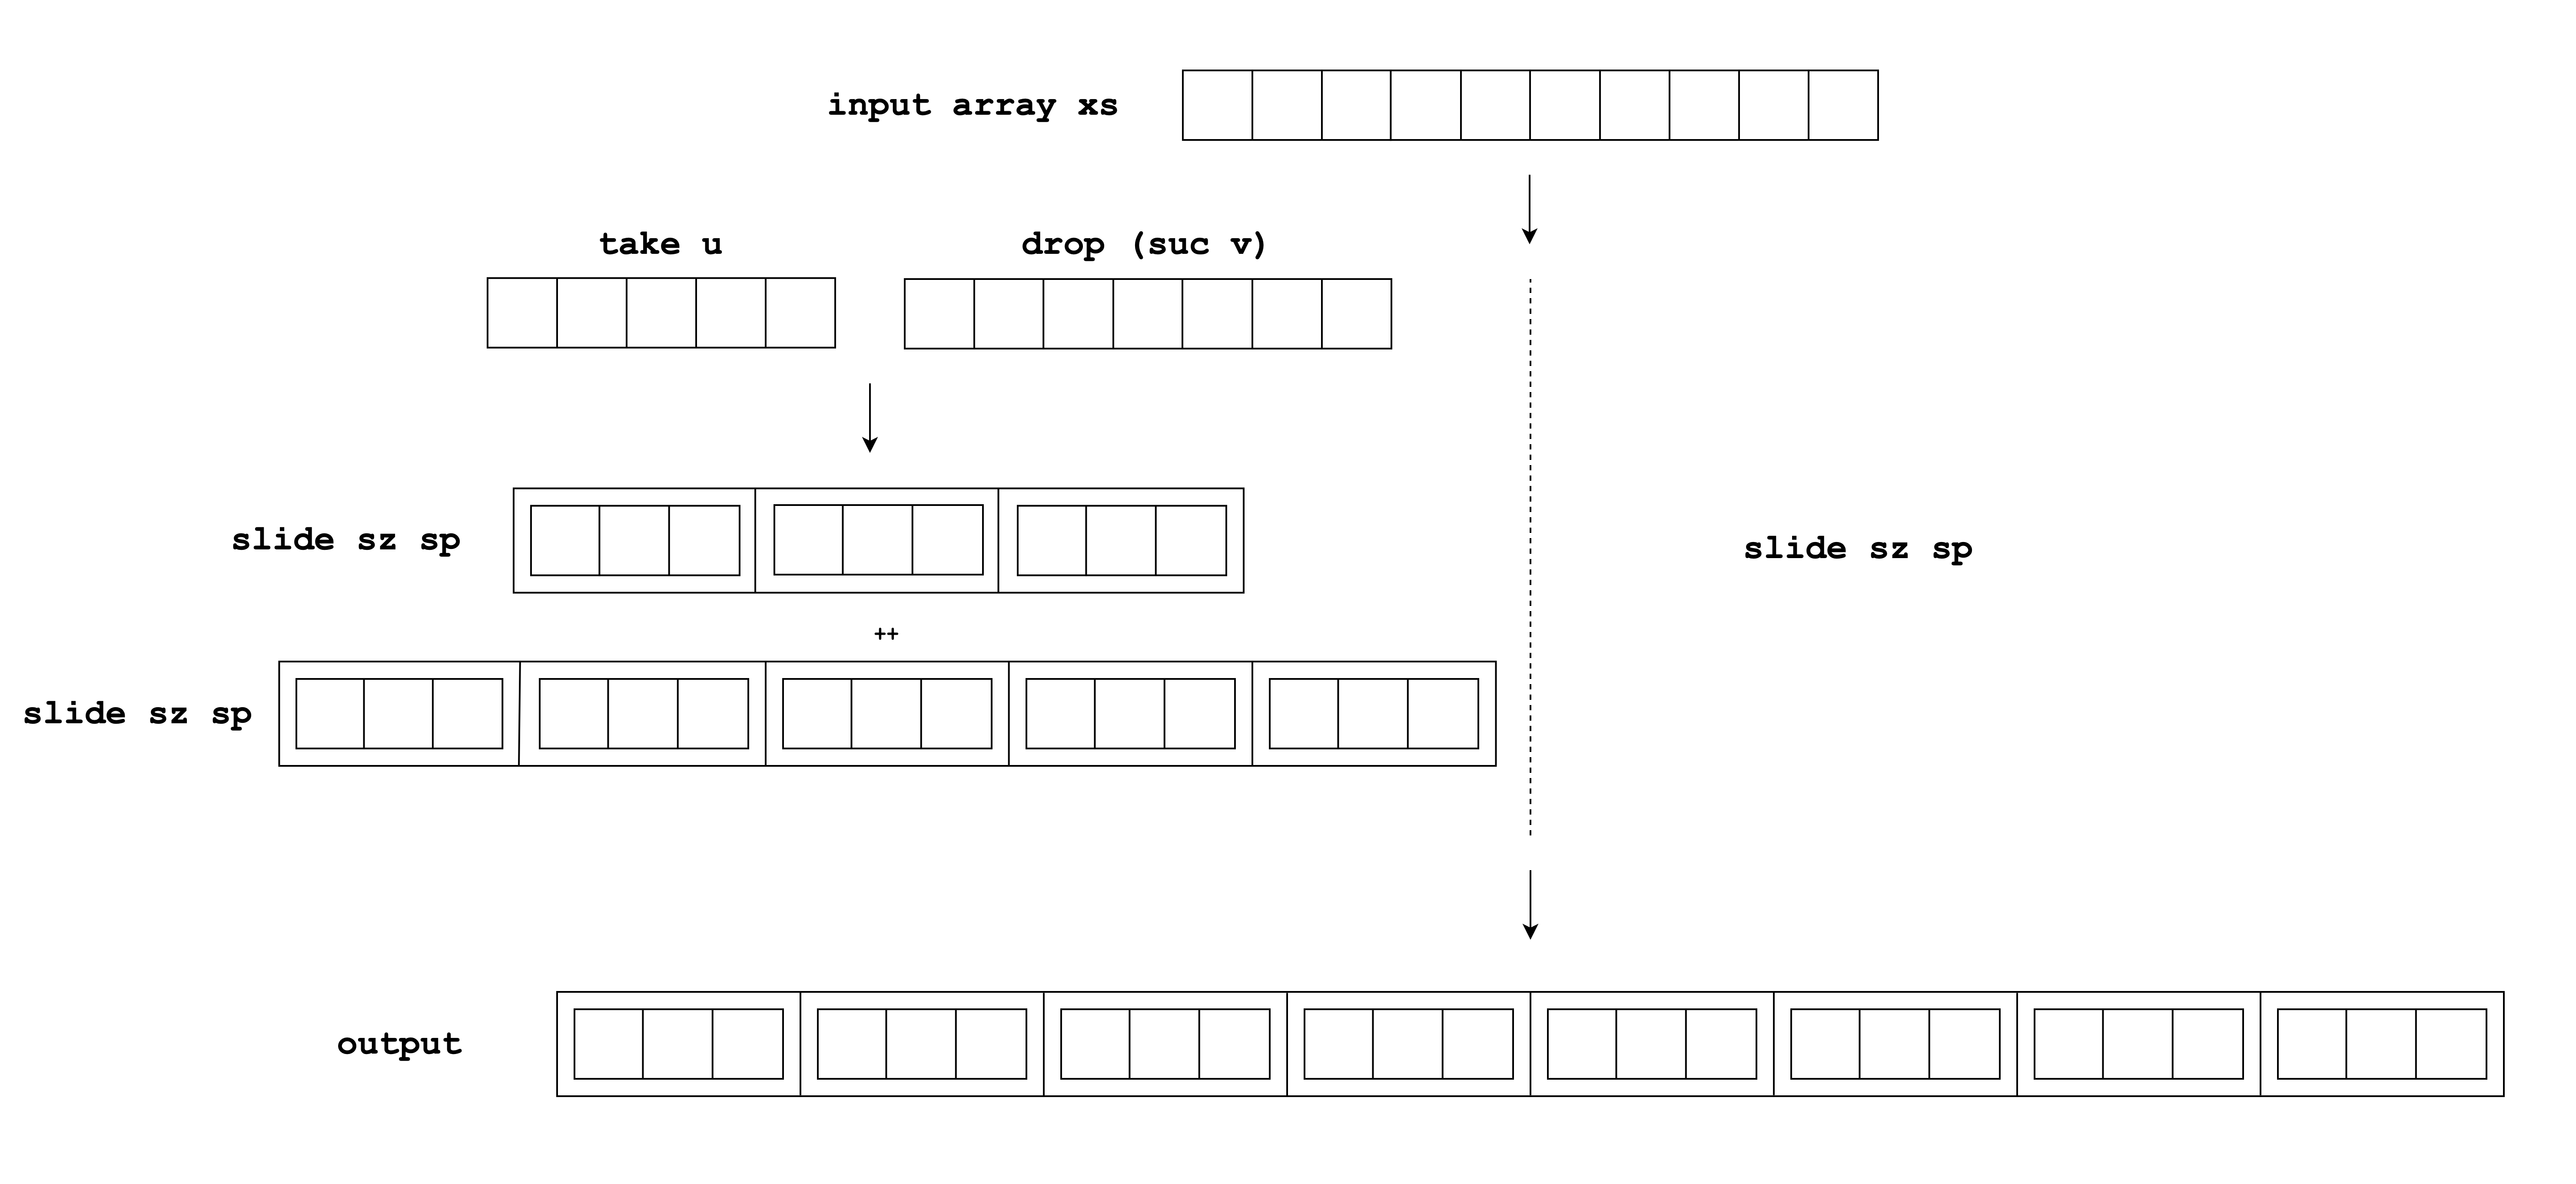
\includegraphics[width=1.0\textwidth]{./images/slideExample.png}
    \caption{An example for illustrating \AgdaPostulate{lem₄}}
    \label{fig:lem4eg}
\end{figure}

In this example, $sz = 3$, $suc\; sp = 1$, $u = 5$ and $suc\; v = 3$, it clearly shows that the result we get from the left-hand side of the lemma \AgdaPostulate{lem₄} equals to the result of the right-hand side.

\subsection{Summary}
\label{stencil:summary}
In this section, we provide the verification of an complex stencil computation rule in Agda. Advantages of machine verification are obvious. Firstly, we make use of the dependently typed pattern matching in Agda to introduce general restrictions on the choices of $u$ and $v$ in the tiling rule \ref{stencil:tiling}. Comparing to the original piece of information we have, i.e., the difference between $u$ and $v$ should equal to the difference between $size$ and $step$, this accurate formalisation can be helpful to eliminate errors in the implementation. Moreover, this complex rule is broken down into smaller rules and justified step by step in a clear structure.

However, the dependently typed pattern matching in Agda also has its limitations. We have to keep doing equality reasoning on arrays' sizes using the properties of natural number addition and multiplication while developing proofs. In the last lemma \AgdaPostulate{lem₄}, since casting the input array's size over complicates the declaration, we have so far not been able to develop a proof although in mathematical form it can be justified.

%==================================================================================================================================
\chapter{Research Outcomes} 
\label{ch:outcomes}
In this project, some important LIFT data types and a large set of primitive operations have been encoded in Agda, and a set of mechanical proofs have been developed to verified the correctness of three categories of rewrite rules: algorithmic rules, movement rules and the stencil computation rule. In general, most of the rules have been proven correct, the incorrect proof and definition have been revised, and inaccurate definitions of arguments' patterns have been clarified. In general, we find machine verification is helpful for formalising and verifying these rewrite rules for optimising the efficiency of array and multi-dimensional array operations.

Induction is the core of the construction of semantics and proofs. It is effective for giving clear structural definitions of data types and primitives as well as constructing reasoning chains in proofs. Agda is helpful for formalising semantics and proofs following proposition-as-type interpretation since it is dependently typed, however this feature also introduces complexities in pattern matching. Some strategies are introduced for resolving these complexities, such as casting patterns at constructor level with equality reasoning with \texttt{cast} defined in section \ref{prim:stencil}; using \texttt{REWRITE} to increase the flexibility of pattern matching while ensuring the soundness of the type system (section \ref{prim:rewrite}); and proving the equality between two expression with different types with heterogeneous equality (section \ref{move:heter}).

Some strategies of constructing proofs are also discussed. A complex rule can be broken down into smaller rules, for example, the tiling rule \ref{stencil:tiling} is proven using two rules moving the $\texttt{map}\; f$ operation into suitable order, and the $\texttt{slideJoin}$ rule to provide the algorithmic justification. Effective lemmas can be defined according to the definitions of primitives, for example, reasoning on expressions containing \texttt{split} can always be proven using lemmas specifying properties of \texttt{take} and \texttt{drop} since \texttt{split} is defined using them (\ref{lift:take}). Also, as the proofs discussed in section \ref{move:join}, section \ref{move:split} and section \ref{move:slide}, some rules are internally related to each other, when one of them is proven, the verification of others can be developed based on the proven ones.

%==================================================================================================================================
\chapter{Conclusion and Future Work}
\label{ch:conclusion}
Effective mechanical verification in Agda is developed for justifying the correctness of the rewrite rules in LIFT. Most of the rewrite rules are proven to be correct while some incorrect or inaccurate rules are adjusted and clarified.

We give brief introduction in chapter \ref{ch:into} about the motivations and aims of the project, and provide background information of LIFT, Agda as well as the computation model Curry-Howard Correspondence in chapter \ref{ch:background}. In chapter \ref{ch:semantics}, encoding LIFT's data types and primitives into operational semantics in Agda is introduced. In chapter \ref{ch:proofs}, we discuss in detail about the development of verification for algorithmic rules, movement rules and the stencil computation rule using proof by induction. The outcomes together with what we have learned in this project are discussed in chapter \ref{ch:outcomes}.

In current stage, we are not able to prove the last lemma used in proving the tiling rule (\ref{stencil:tiling}) in section \ref{sec:stencil} due to the over-complicated pattern matching on the sizes of arrays. It would be interesting for us to research on strategies to simplify these tedious pattern matching in complex multi-dimensional array operations under dependently typed theorem provers like Agda. The \texttt{REWRITE} feature discussed in section \ref{prim:rewrite} can be useful, however its usage is very limited since it can damage the confluence of the type system and affect the termination of programs.

We would also like to explore the restrictions and justify the correctness of applying similar tiling rules in 2D arrays, with stencil computation primitives for 2D arrays, e.g., \texttt{slide\textsubscript{2}} and \texttt{padCst\textsubscript{2}}, and potentially generalise the verification on rules defined for n-dimensional arrays.


%==================================================================================================================================
%
% 
%==================================================================================================================================
%  APPENDICES  

%\begin{appendices}

%\chapter{Appendices}

%Typical inclusions in the appendices are:

%\begin{itemize}
%\item
%  Copies of ethics approvals (required if obtained)
%\item
%  Copies of questionnaires etc. used to gather data from subjects.
%\item
%  Extensive tables or figures that are too bulky to fit in the main body of
%  the report, particularly ones that are repetitive and summarised in the body.
%
%\item Outline of the source code (e.g. directory structure), or other architecture %documentation like class diagrams.
%
%\item User manuals, and any guides to starting/running the software.
%
%\end{itemize}

%\textbf{Don't include your source code in the appendices}. It will be
%submitted separately.
%
%\end{appendices}

%==================================================================================================================================
%   BIBLIOGRAPHY   

% The bibliography style is abbrvnat
% The bibliography always appears last, after the appendices.

\bibliographystyle{abbrvnat}

\bibliography{l4proj}

\end{document}
